\documentclass[a4paper, 11pt, openright]{book} % book template, paper size is b5

%%%%%%%%%%%%%%%%%%%%%%%%%%%%%%%%%%%%%%%%%%%%%%%%%%%%%%%%%%%%%%%%%%%%%%%%%%%%%%%%
% PACKAGES %%%%%%%%%%%%%%%%%%%%%%%%%%%%%%%%%%%%%%%%%%%%%%%%%%%%%%%%%%%%%%%%%%%%%
%%%%%%%%%%%%%%%%%%%%%%%%%%%%%%%%%%%%%%%%%%%%%%%%%%%%%%%%%%%%%%%%%%%%%%%%%%%%%%%%

% Suppress some warnings -------------------------------------------------------
\usepackage{silence}
\WarningsOff[everypage] % Suppress warnings related to package everypage
%\pdfsuppresswarningpagegroup=1

% Maths ------------------------------------------------------------------------
\usepackage{amsmath}             % principal package for serious mathematical typesetting
\usepackage{mathtools}           % improved version of amsmath
\usepackage{amssymb}             % particular mathematical symbols
\usepackage{bm}                  % bold math formula, similar to '\mathbf'
\usepackage{mathrsfs}            % math upper case letter fonts
%\usepackage{scalerel}            % scale/stretch/shift an object to conform a second one
%\usepackage{amsfonts}            % particular mathematical fonts
\usepackage{amsthm}              % to define theorems, lemmas, etc
\usepackage{thmtools}            % to define theorems, lemmas, etc
%\usepackage{mathrsfs}            % math upper case letter fonts
%\usepackage{systeme}             % easy way to write systems of equations
%\usepackage{accents}             % particular accents in math
%\usepackage{commath}             % differential, partial differ., delimiters, etc

\declaretheoremstyle[
  headfont=\normalfont\bfseries,
  notefont=\normalfont\bfseries\itshape,
  bodyfont=\itshape,
  numbered=unless unique,
  spaceabove=1.0em plus 0.25em minus 0.25em,
  qed={$\blacksquare$}, %\qedsymbol
  spacebelow=1.0em plus 0.25em minus 0.25em,
]{defstyle}

\declaretheorem[
  style=defstyle,
  title=Definition,
  refname={definition},
  Refname={Definition}
]{definition}

\declaretheoremstyle[
  headfont=\normalfont\bfseries,
  notefont=\normalfont\bfseries\itshape,
  bodyfont=\normalfont,
  numbered=unless unique,
  spaceabove=1.0em plus 0.25em minus 0.25em,
  qed={$\blacksquare$}, %\qedsymbol
  spacebelow=1.0em plus 0.25em minus 0.25em,
]{exstyle}

\declaretheorem[
  style=exstyle,
  title=Example,
  refname={example},
  Refname={Example}
]{example}

% Document settings ------------------------------------------------------------
\usepackage{geometry}            % change margins of the document
\usepackage{acronym}             % to define abbreviations
\usepackage{rotating}            % rotate objects
%\usepackage{changepage}          % adjust width environment
%\usepackage{enumerate}           % basic generate list with numbered items
%\usepackage{stackengine}         % stack objects vertically
%\usepackage{setspace}            % spacing between lines in a document
%\usepackage{pdfpages}            % for the inclusion of multi-page external PDF documents

% Text settings ----------------------------------------------------------------
\usepackage[dvipsnames]{xcolor}  % color the text
\usepackage{soul}                % to strike-through text
\usepackage{tcolorbox}           % create a colored box wrapping the text
\usepackage[final]{microtype}    % improves the spacing between words and letters
\usepackage[toc, page]{appendix} % to create appendices
\usepackage[english]{babel}      % useful to interpret the language of the document
\usepackage[utf8]{inputenc}      % to correctly write accented letter and other symbols
\usepackage[T1]{fontenc}         % to write correctly in Italian
%\usepackage[latin1]{inputenc}    % codec input useful to write docs in Italian
%\usepackage[normalem]{ulem}      % underline command which will break over line ends
\usepackage{listings}            % to include code in the document
\usepackage{realboxes}           % to create boxes around text
\usepackage{url}                 % to write url in the document

\urlstyle{tt}                    % tt font of the document (forced in the bibliography)
\lstset{                         % settings for the listings package
  basicstyle=\ttfamily,
  columns=fullflexible,
  keepspaces=false
}
\lstnewenvironment{mapleinline}[1][]
  {\lstset{
    frame=none,
    linewidth=1.0\textwidth,
    belowskip=-0.5em,
    #1
  }}{}
\lstnewenvironment{mapleboxed}[1][]
  {\lstset{
    frame=shadowbox,
    linewidth=1.0\textwidth,
    belowskip=-0.5em,
    #1
  }}{}
\lstnewenvironment{maplefigure}[1][]
  {\lstset{
    frame=none,
    linewidth=1.0\textwidth,
    aboveskip=-0.1em,
    belowskip=-0.1em,
    #1
  }}{}

% Fonts ------------------------------------------------------------------------
\usepackage{lmodern}             % text font
%\usepackage{mathspec}            % font selection for XeLaTeX
%\defaultfontfeatures{Mapping=tex-text}       % to support TeX conventions
%\setallmainfonts{Adobe Caslon Pro}           % normal document font
%\setallsansfonts[Scale=1.0]{Montserrat}      % Optima % sans-serif font (\textsf{})
%\setallmonofonts[Scale=0.75]{JetBrains Mono} % mono spaced font (\texttt{})
\usepackage[it,bf]{titlesec}
%\titleformat*{\chapter}{\center\bfseries\LARGE}
\titleformat
{\chapter}                       % command
[display]                        % shape
{\normalfont\center\Huge\bfseries}      % format
{\chaptertitlename\ \thechapter\\[2.5ex]---} % label
{2.5ex}                           % sep
{\Huge}[\vspace{2ex}]  % before-code
%\titleformat*{\section}{\normalfont\bfseries\Large}
%\titleformat*{\section}{}
%\titleformat*{\subsection}{}
\usepackage{textgreek}           % to write greek letters in text mode
%\usepackage{fontawesome}         % to use icons in the document

% Units ------------------------------------------------------------------------
\usepackage{siunitx}             % write unit of measurements

% Citations --------------------------------------------------------------------
\usepackage{hyperref}            % generate hyper-reference links in the pdf document
\usepackage{cleveref}            % to reference equations, figures, tables, etc
%\usepackage{cite}               % lists of numerical citations and representation issues
%\usepackage{authblk}            % to define authors footstep

% Figures and tables -----------------------------------------------------------
\usepackage{graphicx}            % advanced package to load figures
\usepackage{booktabs}            % enhance table quality: midrule, toprule, etc
\usepackage{tabularx}            % to create tables with a fixed width
\usepackage{array}               % array and tabular environments
\usepackage{float}               % improve the interface to define figs and tables
\usepackage{multirow}            % multi rows cells in a table
\usepackage{longtable}           % long tables
\usepackage{makecell}            % to make cells in a table
\usepackage{multicol}            % multi columns cells in a table
\usepackage{caption}             % to customize the captions in floating environments
\usepackage{subcaption}          % again used to customize the captions
\usepackage{overpic}             % to put text over a figure
%\usepackage{subfig}              % generating subfigures
%\usepackage{background}          % to put a background image in the document
%\usepackage{ctable}              % alignement of folats objects
%\usepackage{graphics}            % base package to load figures
\newcolumntype{Y}{>{\centering\arraybackslash}X}
\renewcommand{\theadalign}{cl}
\renewcommand{\cellalign}{cl}

% Algorithms and code ----------------------------------------------------------
\usepackage{algpseudocode}       % to write algorithms
\usepackage{algorithm}           % to write algorithms
\usepackage{algorithmicx}        % to write algorithms

\algnewcommand{\IfThen}[2]{% \IfThenElse{<if>}{<then>}
  \State \algorithmicif\ #1\ \algorithmicthen\ #2}
\algnewcommand{\IfThenElse}[3]{% \IfThenElse{<if>}{<then>}{<else>}
  \State \algorithmicif\ #1\ \algorithmicthen\ #2\ \algorithmicelse\ #3}

\makeatletter
\newenvironment{breakablealgorithm}
  {% \begin{breakablealgorithm}
    \begin{center}
      \refstepcounter{algorithm}% New algorithm
      \hrule height.8pt depth0pt \kern2pt% \@fs@pre for \@fs@ruled
      \renewcommand{\caption}[2][\relax]{% Make a new \caption
        {\raggedright\textbf{\ALG@name~\thealgorithm} ##2\par}%
        \ifx\relax##1\relax % #1 is \relax
          \addcontentsline{loa}{algorithm}{\protect\numberline{\thealgorithm}##2}%
        \else % #1 is not \relax
          \addcontentsline{loa}{algorithm}{\protect\numberline{\thealgorithm}##1}%
        \fi
        \kern2pt\hrule\kern2pt
      }
  }{% \end{breakablealgorithm}
      \kern2pt\hrule\relax% \@fs@post for \@fs@ruled
    \end{center}
  }
\makeatother

% TikZ and PGFPlots ------------------------------------------------------------
\usepackage{tikz}                % to draw figures
\usepackage{pgfplots}            % external TikZ/PGF plots support
\usepgfplotslibrary{fillbetween} % fill the area between two curves
\pgfplotsset{compat=newest}      % compatibility mode
\pgfplotsset{plot coordinates/math parser=false} % to avoid math parser
\usepgfplotslibrary{external}    % load the externalization library
\usetikzlibrary{external}        % use the externalization library
%\tikzexternalize[mode=list and make, prefix=gfx/ext-tikz/]
\usepgfplotslibrary{colorbrewer} % colorbrewer library
\pgfplotsset{colormap/PuOr-4}    % colormap for the plots
\pgfkeys{/pgf/number format/.cd,1000 sep={}} % no thousand separator in the plots
\tikzexternalize[mode=convert with system call, prefix=figures/externalized/]

% layers definition
\pgfplotsset{
  layers/my layer set/.define layer set={
    main,
    back,
    middle,
    front,
  }{}
}

% include tikz images and set externalization filename
\newcommand{\includetikz}[1]{%
  % substitute dots and slash in filename with underscores
  \StrSubstitute{#1}{./}{}[\temp]%
  \StrSubstitute{\temp}{.}{_}[\temp]%
  \StrSubstitute{\temp}{/}{_}[\temp]%
  \tikzsetnextfilename{\temp}%
  \input{#1}%
}

%%%%%%%%%%%%%%%%%%%%%%%%%%%%%%%%%%%%%%%%%%%%%%%%%%%%%%%%%%%%%%%%%%%%%%%%%%%%%%%%
% DOCUMENT SETUP %%%%%%%%%%%%%%%%%%%%%%%%%%%%%%%%%%%%%%%%%%%%%%%%%%%%%%%%%%%%%%%
%%%%%%%%%%%%%%%%%%%%%%%%%%%%%%%%%%%%%%%%%%%%%%%%%%%%%%%%%%%%%%%%%%%%%%%%%%%%%%%%

% Set custom margins for the document ------------------------------------------
\newgeometry{top=1.25in, bottom=1.0in, left=1.0in, right=1.0in} % digital version
%\newgeometry{top=2.0cm, bottom=2.0cm, width=11cm, bindingoffset=12mm} % print version
%headsep=0.25in, headheight=20pt, heightrounded

% Write 10^0 instead of 1 (requires 'siunitx') ---------------------------------
\sisetup{retain-zero-exponent=false}

% Modify layout of command SIrange (requires 'siunitx') ------------------------
\sisetup{range-phrase = \text{ -- }}

% Set the indent length to zero ------------------------------------------------
\setlength\parindent{0pt}
\setlength\itemsep{0pt}

% Set the path of the figure files ---------------------------------------------
\graphicspath{
  {figures/frontmatter/}
  {figures/chapter_1/}
  {figures/chapter_2/}
  {figures/chapter_3/}
  {figures/chapter_4/}
  {figures/chapter_5/}
  {figures/chapter_6/}
  {figures/chapter_7/}
  {figures/appendix_1/}
}

% Insert a date ----------------------------------------------------------------
\date{January 2024}

% Bibliography -----------------------------------------------------------------
\PassOptionsToPackage{%
  backend=biber, bibencoding=utf8, % instead of bibtex
  %backend=bibtex8,bibencoding=ascii, %
  language=auto, %
  style=numeric-comp, %
  %style=authoryear-comp, % Author 1999, 2010
  %bibstyle=authoryear, dashed=false, % dashed: substitute rep. author with ---
  sorting=none, % sorted by appearance
  maxbibnames=10, % default: 3, et al.
  %backref=true, %
  natbib=true, % natbib compatibility mode (\citep and \citet still work)
}{biblatex}
\usepackage{biblatex} % to display bibliography
\usepackage{bibentry} % to insert bibliography entries inline
\emergencystretch=1em
\addbibresource{bibliography.bib}

% Reduce the margin of the summary/abstract ------------------------------------
%\def\changemargin#1#2{
%  \list{}{\rightmargin#2\leftmargin#1}
%  \item[]}
%\let\endchangemargin=\endlist

%%%%%%%%%%%%%%%%%%%%%%%%%%%%%%%%%%%%%%%%%%%%%%%%%%%%%%%%%%%%%%%%%%%%%%%%%%%%%%%%
% DEFINITIONS OF COMMANDS AND VARIABLES %%%%%%%%%%%%%%%%%%%%%%%%%%%%%%%%%%%%%%%%
%%%%%%%%%%%%%%%%%%%%%%%%%%%%%%%%%%%%%%%%%%%%%%%%%%%%%%%%%%%%%%%%%%%%%%%%%%%%%%%%

% Create the 'abstract' environment (not present by default in the 'book' class)
\newcommand{\summaryname}{Abstract}
\newenvironment{Abstract}{
  \begin{center}
    \bfseries{\summaryname}
  \end{center}
}

% Definitions of new table columns commands (require package 'array') ----------
\newcolumntype{L}[1]{>{\raggedright\let\newline\\\arraybackslash\hspace{0pt}}m{#1}}
\newcolumntype{C}[1]{>{\centering\let\newline\\\arraybackslash\hspace{0pt}}m{#1}}
\newcolumntype{R}[1]{>{\raggedleft\let\newline\\\arraybackslash\hspace{0pt}}m{#1}}
\newcolumntype{P}[1]{>{\centering\arraybackslash}p{#1}}
\newcolumntype{M}[1]{>{\centering\arraybackslash}m{#1}}

% Definitions of mathematical commands to typeset many things ------------------

\newtheorem{observation}{Observation}
\newtheorem{remark}{Remark}

% General commands
\newcommand{\eg}{\emph{e.g.}}
\newcommand{\ie}{\emph{i.e.}}
\newcommand{\pow}{\ensuremath{^{\wedge}}}
\newcommand{\SSI}[2]{\SI[per-mode=symbol]{#1}{#2}}
\newcommand{\RSI}[3]{\lbrack\num{#1}{,}\ \num{#2}\rbrack\,\si[per-mode=symbol]{#3}}

% Software programs
\newcommand{\MapleSoft}{\textsc{Maplesoft}\textsuperscript{\textregistered}}
\newcommand{\Maple}{\textsc{Maple}\textsuperscript{\textregistered}}
\newcommand{\Wolfram}{\textsc{Wolfram}}
\newcommand{\Mathematica}{\textsc{Mathematica}\textsuperscript{\textregistered}}
\newcommand{\Matlab}{\textsc{Matlab}\textsuperscript{\textregistered}}
\newcommand{\Simulink}{\textsc{Simulink}\textsuperscript{\textregistered}}
\newcommand{\Mex}{\textsc{Mex}}
\newcommand{\SFunction}{\textsc{S-Function}}
\newcommand{\Axiom}{\textsc{Axiom}}
\newcommand{\Derive}{\textsc{Derive}}
\newcommand{\Macsyma}{\textsc{Macsyma}}
\newcommand{\MuPAD}{\textsc{MuPAD}}
\newcommand{\Reduce}{\textsc{Reduce}}
\newcommand{\TrussMe}{\textsc{TrussMe-Fem}}
\newcommand{\Ansys}{\textsc{Ansys}\textsuperscript{\textregistered}}

% Miscellaneous libraries, languages and tools
\newcommand{\cpp}{C++}
\newcommand{\html}{HTML}
\newcommand{\CGAL}{CGAL}
\newcommand{\LEM}{LEM}
\newcommand{\SIG}{SIG}
\newcommand{\LAST}{LAST}
\newcommand{\LULEM}{\texttt{LULEM}}
\newcommand{\Indigo}{\textsc{Indigo}}
\newcommand{\Doxygen}{\textsc{Doxygen}}
\newcommand{\Sphinx}{\textsc{Sphinx}}
\newcommand{\CMake}{\textsc{CMake}}
\newcommand{\Const}{\textsc{Const}}
\newcommand{\SharedPointer}{\textsc{SharedPointer}}

% Eigen namespace and classes
\newcommand{\Eigen}{\textsc{Eigen}}
\newcommand{\MatrixBase}{\textsc{MatrixBase}}

% Acme namespace and classes
\newcommand{\Acme}{ACME}
\newcommand{\Entity}{\textsc{Entity}}
\newcommand{\Entities}{\textsc{Entities}}
\newcommand{\Point}{\textsc{Point}}
\newcommand{\Line}{\textsc{Line}}
\newcommand{\Ray}{\textsc{Ray}}
\newcommand{\Plane}{\textsc{Plane}}
\newcommand{\Segment}{\textsc{Segment}}
\newcommand{\Triangle}{\textsc{Triangle}}
\newcommand{\Disk}{\textsc{Disk}}
\newcommand{\Ball}{\textsc{Ball}}
\newcommand{\Collection}{\textsc{Collection}}
\newcommand{\Aabb}{\ac{AABB}}
\newcommand{\AabbTree}{\ac{AABB}\textsc{tree}}

% Enve namespace and classes
\newcommand{\Enve}{\textsc{Enve}}
\newcommand{\TriangleGround}{\textsc{TriangleGround}}
\newcommand{\Mesh}{\textsc{Mesh}}
\newcommand{\Flat}{\textsc{Flat}}
\newcommand{\Rib}{\textsc{Rib}}
\newcommand{\Shape}{\textsc{Shape}}
\newcommand{\Shell}{\textsc{Shell}}
\newcommand{\Tire}{\textsc{Tire}}
\newcommand{\Road}{\textsc{Road}}

% Tire models
\newcommand{\MagicFormulae}{\textsc{Magic Formula}}
\newcommand{\Swift}{\textsc{Swift}\textsuperscript{\textregistered}}
\newcommand{\TMEasy}{\textsc{TMEasy}}
\newcommand{\FTire}{\textsc{FTire}\textsuperscript{\textregistered}}
\newcommand{\CDTire}{\textsc{CDTire}\textsuperscript{\textregistered}}

% Goodlooking check, cross and warning marks
%\newcommand{\mycheckmark}{\textcolor{mycolor5}{\faCheck}}
%\newcommand{\mycrossmark}{\textcolor{mycolor2}{\faTimes}}
%\newcommand{\mywarnmark}{\textcolor{mycolor3}{\faExclamationTriangle}}

% Mathematical symbols
\newcommand{\code}[1]{\texttt{#1}}
\newcommand{\pt}[1]{\ensuremath{\mathbf{#1}}}
\newcommand{\vt}[1]{\ensuremath{\vec{\pt{#1}}}}
\newcommand{\et}[1]{\ensuremath{\hat{\pt{#1}}}}

\newcommand{\sett}[1]{\ensuremath{\mathcal{#1}}}
\newcommand{\boundary}[1]{\ensuremath{\partial{\sett{#1}}}}
\newcommand{\interior}[1]{\ensuremath{\mathring{\sett{#1}}}}

\newcommand{\de}{\mathrm{d}}

% Matrices and vectors
\newcommand{\m}[1]{\ensuremath{\mathbf{#1}}}
\newcommand{\mx}{\ensuremath{\m{x}}}
\newcommand{\mxp}{\ensuremath{\mx^\prime}}
\newcommand{\mE}{\ensuremath{\m{E}(\mx, t)}}
\newcommand{\mg}{\ensuremath{\m{g}(\mx, t)}}
\newcommand{\ma}{\ensuremath{\m{a}(\mx, t)}}
\newcommand{\mv}{\ensuremath{\m{v}(\mx, t)}}
\newcommand{\mA}{\ensuremath{\m{A}(\mx, t)}}
\newcommand{\mN}{\ensuremath{\m{N}(\mx, t)}}
\newcommand{\mK}{\ensuremath{\m{K}(\mx, t)}}
\newcommand{\mI}{\ensuremath{\m{I}}}
\newcommand{\mP}{\ensuremath{\m{P}}}
\newcommand{\mQ}{\ensuremath{\m{Q}}}
\newcommand{\mL}{\ensuremath{\m{L}(\mx, t)}}
\newcommand{\mU}{\ensuremath{\m{U}(\mx, t)}}
\newcommand{\mM}{\ensuremath{\m{M}(\mx, t)}}
\newcommand{\mb}{\ensuremath{\m{b}(\mx, t)}}
\newcommand{\mAd}{\ensuremath{\m{E}_{\m{a}}(\mx, t)}}
\newcommand{\mgd}{\ensuremath{\m{g}_{\m{a}}(\mx, t)}}
\newcommand{\mF}{\ensuremath{\m{F}(\mx, \mxp, t)}}
\newcommand{\mh}{\ensuremath{\m{h}(\mx, t)}}
\newcommand{\mV}{\ensuremath{\m{v}(\mx, t)}}

\newcommand{\mq}{\ensuremath{\m{q}}}
\newcommand{\mqd}{\ensuremath{\m{{q}^{\prime}}}}
\newcommand{\mqdd}{\ensuremath{\m{{q}^{\prime\prime}}}}
\newcommand{\ml}{\ensuremath{\boldsymbol{\lambda}}}

\newcommand{\cf}{\ensuremath{\,\mathrm{f}}}
\newcommand{\cm}{\ensuremath{\,\mathrm{m}}}
\newcommand{\cd}{\ensuremath{\,\mathrm{d}}}
\newcommand{\ca}{\ensuremath{\,\mathrm{a}}}



\newcommand{\eqdef}{\mathrel{\overset{\makebox[0pt]{\mbox{\normalfont\tiny def}}}{=}}}
\newcommand{\bfell}{\ensuremath{\mathcal{L}}}
\newcommand{\huvec}{\ensuremath{\hat{\mathbf{n}}}}
\newcommand{\euvec}{\ensuremath{\hat{\mathbf{e}}}}
\newcommand{\road}{\ensuremath{\mathcal{R}}}
\newcommand{\tire}{\ensuremath{\mathcal{T}}}
\newcommand{\cp}{\ensuremath{\mathcal{P}}}
\newcommand{\adh}{\ensuremath{\mathcal{A}}}
\newcommand{\sli}{\ensuremath{\mathcal{S}}}

\newcommand{\mini}{\ensuremath{\mathrm{\min}}}
\newcommand{\maxi}{\ensuremath{\mathrm{\max}}}
\newcommand{\meai}{\ensuremath{\mathrm{\mu}}}
\newcommand{\vari}{\ensuremath{\mathrm{\sigma^2}}}

\newcommand{\Fiala}{\textsc{Fiala}}
\newcommand{\NeoFiala}{\textsc{Neo-Fiala}}
\newcommand{\TreadSim}{\textsc{TreadSim}}
\newcommand{\TaMeTire}{\textsc{TaMeTire}\textsuperscript{\textregistered}}
\newcommand{\Hoosier}{\textsc{Hoosier}\textsuperscript{\textregistered}}

% Commands for the structural analysis
\newcommand{\Je}{\mathbf{J}_{e}}
\newcommand{\Ke}{\mathbf{K}_{e}}
\newcommand{\Ne}{N_{e}}
\newcommand{\Pe}{\mathbf{P}_{e}}
\renewcommand{\Re}{\mathbf{R}_{e}}
\newcommand{\Te}{\mathbf{T}_{e}}
%\newcommand*\circled[1]{\tikz[baseline=(char.base)]{\node[shape=circle,draw,inner sep=2pt] (char) {#1};}}
\newcommand*\circled[1]{{\large \textcircled{\small #1}}}

% Matlab colors
\definecolor{mycolor1}{rgb}{0.00000,0.44700,0.74100}
\definecolor{mycolor2}{rgb}{0.85000,0.32500,0.09800}
\definecolor{mycolor3}{rgb}{0.92900,0.69400,0.12500}
\definecolor{mycolor4}{rgb}{0.49400,0.18400,0.55600}
\definecolor{mycolor5}{rgb}{0.46600,0.67400,0.18800}
\definecolor{mycolor6}{rgb}{0.30100,0.74500,0.93300}
\definecolor{mycolor7}{rgb}{0.63500,0.07800,0.18400}

% Pages numbering --------------------------------------------------------------
\makeatletter
\newcommand*{\emptystyles}{% remove page style
\let\oldplain\ps@plain
\let\ps@plain\ps@empty
\pagestyle{empty}}

\newcommand*{\restorestyles}{% restore page style
\clearpage\thispagestyle{empty}
\let\ps@plain\oldplain
\pagestyle{headings}}

\let\ps@plain\ps@empty% remove page numbers from chapter pages
\makeatother

%%%%%%%%%%%%%%%%%%%%%%%%%%%%%%%%%%%%%%%%%%%%%%%%%%%%%%%%%%%%%%%%%%%%%%%%%%%%%%%%
% BEGIN DOCUMENT %%%%%%%%%%%%%%%%%%%%%%%%%%%%%%%%%%%%%%%%%%%%%%%%%%%%%%%%%%%%%%%
%%%%%%%%%%%%%%%%%%%%%%%%%%%%%%%%%%%%%%%%%%%%%%%%%%%%%%%%%%%%%%%%%%%%%%%%%%%%%%%%

\begin{document}

% Frontmatter ------------------------------------------------------------------
\emptystyles
%!TEX root = ../main.tex

\begin{titlepage}
%
\setlength\parindent{0pt}
\setlength{\topmargin}{-20mm}
\setlength{\voffset}{0mm}
%
\begin{center}
  \rule[0.1cm]{\textwidth}{0.6mm} \\ % horizontal lines
  \rule[0.5cm]{\textwidth}{0.3mm}
\end{center}
%
\vspace{-5mm}
%
\begin{figure}[h]
  \centering
  
\includegraphics[scale=0.5]{./figures/frontmatter/logo.png}
\end{figure}
%
\begin{center}
  %\LARGE{\textsc{University of Trento}} \\
  \Large{\textsc{Department of Industrial Engineering}} \\
  \vspace{2mm}
  \large{\textsl{Doctoral School in Materials, Mechatronics and Systems Engineering}} \\
  %\large{\text{XXXVI} \textsl{Cycle}}
\end{center}
%
\begin{center}
  \rule[0.1cm]{\textwidth}{0.3mm} \\ % horizontal lines
  \rule[0.5cm]{\textwidth}{0.6mm}
\end{center}
%
\vfill
%
\begin{center}
  \LARGE{\textbf{Symbolic Computation Methods for the Real-Time Numerical Solution of Dynamical Systems}} \\
\end{center}
%
\vfill
%
\begin{minipage}[t]{0.49\textwidth}
  \large{\textsc{Supervisors:}} \\
  Prof.~Enrico Bertolazzi \\[0.05em]
  Prof.~Francesco Biral
\end{minipage}
\hfill
\begin{minipage}[t]{0.49\textwidth}\raggedleft
  \large{\textsc{Ph.D. Candidate:}} \\
  Davide Stocco
  \vspace{5mm}
\end{minipage}
%
\vfill
%
\begin{center}
  \large{\textsc{Academic Year 2022/2023}}
\end{center}

\end{titlepage}
\hbox{}
\thispagestyle{empty}
\newpage

% Copyrigth --------------------------------------------------------------------
\vspace*{\fill}
\begin{center}
  Copyright \textcopyright{} 2024 Davide Stocco \\
\end{center}
\thispagestyle{empty}
\cleardoublepage

% Abstract ---------------------------------------------------------------------
%!TEX root = ../main.tex

\newgeometry{ top=2.5cm,bottom=2.5cm,left=3.7cm,right=3.7cm }
\begin{abstract}

  \acp{DAE} find extensive application in modeling complex systems, including electrical circuits, mechanical systems, chemical reactions, and in solving trajectory-prescribed path control problems and partial differential equations. The differential index of a \ac{DAE} system, indicating the minimum number of differentiations needed to transform it into an equivalent system of \acp{ODE}, serves as an indicator of the system's solution difficulty. Index reduction is a crucial preliminary step in the numerical integration of \acp{DAE}, which reduces the system's complexity significantly and allows the usage of standard \acp{ODE} solvers. Notably, index reduction is critical for addressing high-index \ac{DAE} systems. Conversely, if index reduction is not performed, high-order numerical solvers are required to achieve a low-precision solution to high-index \acp{DAE}. Although closed-form index reduction methods exist for specific \ac{DAE} classes like multi-body systems, reducing the index of generic first-order \ac{DAE} systems can pose challenges, particularly for large systems with many equations and variables.

  This research introduces a novel algorithm designed to reduce the index of generic first-order \acp{DAE}, which are linear in the states' derivatives, employing \acp{CAS} for symbolic equation manipulation. The algorithm uses a repeated application of symbolic matrix factorization to automatically separate differential and algebraic equations, followed by the symbolic differentiation of the separated algebraic equations to decrease by one the \acp{DAE} index. These steps are repeated until deemed necessary, typically until an index-0 \acp{DAE} (\acp{ODE}) or index-1 \acp{DAE} is obtained. Special attention is given to the mitigation of the so-called expression swell, a common issue in symbolic computation that can lead to excessive memory usage and slow computation times. Effective strategies based on hierarchical representations are proposed to address this issue, which affects the symbolic matrix factorization process. These strategies, aimed at easing the computational burden and time, represent advancements in symbolic matrix factorization and \acp{DAE} index reduction techniques.

  The proposed methodology is implemented in the open-source \Indigo{} library, employed for symbolic manipulation of \acp{DAE} in the \Maple{} environment, and for generating optimized code for numerical integration of the reduced system in \Matlab{}. Dependencies on external libraries are limited to the \LEM{} and \LAST{} \Maple{} open-source packages, which enact the symbolic matrix factorization with large expression management. Validation of the algorithm encompasses various benchmark problems, spanning mechanical systems, electrical circuits, trajectory-prescribed path control problems, and artificial \acp{DAE} with arbitrarily high indexes. The results demonstrate its effectiveness in reducing the index of these systems up to an index-11 test, highlighting its robustness across several applications. Furthermore, the generated code for numerical integration exhibits stability and efficiency, showcasing the algorithm's practical utility in real-world scenarios. This capability is particularly significant in the context of complex systems, where reducing the index of generic \acp{DAE} is crucial for accurate simulations. Overall, the proposed method provides users with a reliable means to address the index-reduction of high-index \acp{DAE}, offering a valuable tool for effectively tackling the numerical solution of complex dynamical systems.
\end{abstract}
\restoregeometry
\vspace*{\fill}

% Table of contents ------------------------------------------------------------
\setcounter{secnumdepth}{3}
\setcounter{tocdepth}{2}
\tableofcontents
\restorestyles

% List of figures --------------------------------------------------------------
\cleardoublepage
\phantomsection
\addcontentsline{toc}{chapter}{\listfigurename}
\listoffigures

% List of tables ---------------------------------------------------------------
\cleardoublepage
\phantomsection
\addcontentsline{toc}{chapter}{\listtablename}
\listoftables

% List of abbreviations --------------------------------------------------------
\cleardoublepage
\phantomsection
\addcontentsline{toc}{chapter}{List of Abbreviations}
\chapter*{List of Abbreviations}
\markboth{LIST OF ABBREVIATIONS}{}
\begin{acronym}[XXXXXX]
  \acro{2D}{Two-Dimensional}
  \acro{3D}{Three-Dimensional}
  \acro{BSD}{Berkeley Software Distribution}
  \acro{BC}{Boundary Condition}å
  \acro{ADAS}{Advanced Driver-Assistance Systems}
  \acro{RDF}{Road Data Format}
  \acro{HIL}{Hardware In the Loop}
  \acro{SIL}{Software In the Loop}
  \acro{DIL}{Driver In the Loop}
  \acro{MBS}{Multibody System}
  \acro{MB}{Multibody}
  \acro{FEM}{Finite Element Method}
  \acro{FE}{Finite Element}
  \acro{FEA}{Finite Element Analysis}
  \acro{SRT}{Soft Real-Time}
  \acro{HRT}{Hard Real-Time}
  \acro{RT}{Real-Time}
  \acro{ODE}{Ordinary Differential Equation}
  \acro{DAE}{Differential Algebraic Equation}
  \acro{BLAS}{Basic Linear Algebra Subprograms}
  \acro{LAPACK}{Linear Algebra PACKage}
  \acro{DSM}{Direct Stiffness Method}
  \acro{SA}{Structural Analysis}
  \acro{LU}{Lower-Upper}
  \acro{FFLU}{Fraction-Free Lower-Upper}
  \acro{GJ}{Gauss-Jordan}
  \acro{RTF}{Real-Time Factor}
  \acro{API}{Application Programming Interface}
  \acro{GUI}{Graphical User Interface}
  \acro{CPU}{Central Processing Unit}
  \acro{GPU}{Graphics Processing Unit}
  \acro{RAM}{Random Access Memory}
  \acro{AABB}{Axis-Aligned Bounding Box}
  \acro{BVH}{Bounding Volume Hierarchy}
  \acro{BVP}{Bounding Volume Primitive}
  \acro{OS}{Operative System}
  \acro{UHD}{Ultra High Definition}
  \acro{MF}{\textsc{Magic Formula}}
  \acro{DOF}{Degree of Freedom}
  \acro{RTF}{Real-Time Factor}
  \acro{CAS}{Computer Algebra System}
  \acro{SCAS}{Symbolic Computer Algebra System}
  \acro{SMS}{Symbolic Manipulation System}
  \acro{MPL}{Mathematical Pseudo-Language}
  \acro{CERN}{Conseil Europ{\'e}en pour la Recherche Nucl{\'e}aire}
\end{acronym}

% Mainmatter -------------------------------------------------------------------
%!TEX root = ../main.tex

\chapter{Introduction}
\label{chap1:introduction}

% % % % % % % % % % % % % % % % % % % % % % % % % % % % % % % % % % % % % % % %

\section{Background and Motivation}

In modern engineering practices, the numerical simulation of dynamic systems has become increasingly important, offering invaluable insights into the behavior of complex systems across diverse domains. From automotive engineering to aerospace, robotics, and electrical systems, numerical simulations are indispensable for understanding system behaviors, optimizing performance, and guiding design decisions. Central to many of these simulations are systems described by \acp{ODE} and \acp{DAE}. While \acp{ODE} are relatively straightforward to solve, they have limited applicability in modeling systems with constraints or algebraic relationships~\cite{brenan1995numerical}. \acp{DAE}, on the other hand, provide a more elegant framework for modeling complex systems by combining differential equations with algebraic constraints. This versatility makes \acp{DAE} a powerful tool for modeling a wide range of dynamic systems. However, their solution poses significant challenges due to their inherent mixed differential and algebraic nature. \acp{PDE} and \acp{PDAE} are also used to model dynamic systems. The relationship between \acp{PDAE} and \acp{PDE} is analogous to the relationship between \acp{ODE} and \acp{DAE}. Unsurprisingly, the solution of \acp{PDAE} is also significantly challenging, requiring special discretization techniques to reduce the system to a \acp{DAE}, for which more conventional solution methods can be employed~\cite{dedieuleveult2009global}. Nevertheless, the focus of this research is on \acp{DAE}, which are widely used in engineering applications and present distinctive challenges in terms of numerical integration and solution.

The inherent complexity and possible stiffness of \acp{DAE} pose significant obstacles to achieving fast simulations~\cite{burger2018dae, blundell2004multibody, dejalon1994kinematic}. Additionally, stiff systems, characterized by disparate timescales among variables, demand numerical methods capable of handling rapid changes without sacrificing stability or accuracy. Traditional numerical techniques, like explicit solvers, often fail in these scenarios, necessitating the adoption of implicit methods that lead to higher computational costs~\cite{petzold1982differential, brenan1995numerical}. Within this context, symbolic computation are promising for overcoming the challenges posed by \acp{DAE} in dynamic system simulation. Unlike purely numerical approaches, symbolic computation operates on mathematical expressions in their exact form. Such a capability proves valuable for lowering the structural complexities of \acp{DAE}. Indeed, symbolic techniques can systematically reduce \acp{DAE}' index, transforming them into forms more appropriate for numerical integration. This process not only unwinds the complexity of the equations but also enhances the speed and stability of numerical solvers, thereby improving the overall performance of simulations~\cite{petzold1982differential, brenan1995numerical, griepentrog1986differential}.

A key advantage of symbolic computation lies in its capacity to derive exact or partial solutions for specific components of the system. These solutions can then be leveraged to enhance the efficiency of numerical solvers by generating optimized code or simplifying the equations before numerical integration. By combining symbolic and numerical methods, researchers can exploit the strengths of each approach, thereby achieving the best performance and reliability in simulation. However, this hybrid computational framework does not come without its challenges. Such integration requires careful consideration of the algorithms, data structures, and computational strategies to ensure an optimal implementation. Indeed, symbolic operations cannot always replace numerical methods, as they may be computationally expensive or impractical for large-scale systems. Vice versa, numerical methods may struggle with overly complex symbolic expressions that could be simplified through symbolic computation, hindering the overall efficiency of the simulation. In other words, symbolic computation and numerical methods are complementary tools that carry different information and must be judiciously combined to achieve the much-desired performance improvements~\cite{cohen2002computer, cohen2003computer}. This research aims to close such a gap between symbolic computation and numerical methods, developing a comprehensive framework that leverages the strengths of both approaches to solve \acp{DAE} efficiently and accurately in dynamics simulations applied, but not limited, to vehicle dynamics.

Within the domain of vehicle simulation, the accurate and fast solution of systems described by \acp{DAE} holds paramount importance~\cite{burger2018dae,blundell2004multibody, dejalon1994kinematic, andreasson2016deployment, pankiewicz2003off}. In industries like automotive, the development of \ac{ADAS}, autonomous vehicles, and high-performance cars critically depends on robust simulations. These simulations must accurately account for the far from trivial relationships between mechanical components, control systems, and environmental factors such as driver inputs. As a consequence, vehicle dynamics simulations encounter a plethora of challenges, reflecting the complexity of real-world systems. The willingness to push the boundaries of vehicle performance, safety, and autonomous driving capabilities demands simulations that are not only accurate but also fast. This speed is crucial for \ac{RT} applications, where rapid decision-making and control are essential. Furthermore, \ac{AI} training and validation require extensive simulations. Thereby, faster simulations inherently lead to more efficient training and validation processes~\cite{piccinini2022predictive, piccinini2023physics}. Importantly, the challenges faced in vehicle dynamics simulations are not unique to this field but are representative of the broader challenges in dynamic system simulations. The need for effective simulations is a common theme across various engineering disciplines, highlighting the importance of developing advanced computational techniques.

A fast simulation does not come only from the numerical solver but also from the model's structure and the sub-models that compose it. For instance, in vehicle dynamics simulations, the tire-road interaction is a critical aspect that significantly impacts the overall performance and behavior of the vehicle~\cite{nakajima2019advanced}. The tire model's complexity and the computational cost associated with its simulation are crucial factors in determining the overall simulation speed. Another key aspect is the modeling of the vehicle's structure, which involves the simulation of flexible bodies and joints. The interaction between these components and the environment, such as the road surface, further complicates the simulation. Therefore, developing dedicated algorithms and models can significantly enhance the speed and accuracy of vehicle dynamics simulations~\cite{pankiewicz2003off}. In this regard, this research also aims to address these challenges by compounding the solutions of \acp{DAE} with tire-road interaction and vehicle structure deformation models suitable for \ac{HRT} applications.

% % % % % % % % % % % % % % % % % % % % % % % % % % % % % % % % % % % % % % % %

\section{Objectives and Significance}

The significance of this research lies in its impact on the simulation and analysis of complex dynamic systems, particularly in vehicle dynamics. By developing a hybrid computational framework that combines symbolic computation with numerical methods, this study addresses critical challenges associated with solving \acp{DAE}. The contributions have implications for academic and industrial applications, advancing the state of the art in dynamic system simulation. Specifically, the primary objectives of this thesis and their significance are the following.

\begin{itemize}
  \setlength\itemsep{0.0em}
  %
  \item \textbf{Enhance existing numerical methods with symbolic computation methods} -- This involves creating a robust framework combining numerical and symbolic methods to solve stiff high-index \acp{DAE} effectively. The framework aims to handle the complexities and specific requirements of simulations across various engineering disciplines. Indeed, traditional numerical methods often struggle with the complexity and stiffness of \acp{DAE}, leading to issues such as numerical instability. By integrating symbolic computation techniques, this study seeks to improve the simulation performances by preprocessing and simplifying equations, reducing computational overhead, providing exact solutions for sub-problems, and boosting numerical solvers' overall stability and performance. This results in more reliable and faster simulations, so crucial for advanced engineering systems' design and optimization.
  %
  \item \textbf{Develop and implement new algorithms for \acp{DAE} index reduction} -- The index of a \ac{DAE} serves as a measure of its complexity, with higher-index equations posing numerical challenges. The novel symbolic algorithms for index reduction presented in this thesis provide a systematic approach to transforming high-index \acp{DAE} into a form more suitable for standard numerical methods used with \acp{ODE}. The proposed algorithms are specifically designed to mitigate the expression swell phenomenon, a common issue in symbolic computation that can hinder the efficiency and scalability of the index reduction process. Besides expanding the applicability of numerical solvers to more complex systems, this also preserves the integrity and physical relevance of the original models. The ability to handle high-index \acp{DAE} effectively is particularly relevant in vehicle dynamics, robotics, and control systems, where such equations frequently arise.
  %
  \item \textbf{Validate the proposed methods through real-world simulation scenarios} -- Practical validation is crucial for demonstrating the effectiveness of the proposed methods. This objective involves applying the developed framework and algorithms to real-world simulation problems, such as the dynamics of rigid and flexible \ac{MB} systems, \ac{TPPC} problems, and electrical systems. The proposed methods' performance, accuracy, and computational efficiency are assessed in these contexts.
  %
  \item \textbf{Develop sub-models and techniques for \ac{HRT} vehicle dynamic simulations} -- In addition to the core research objectives, this research aims to develop dedicated algorithms and models for simulating the tire-road interaction and the vehicle's structural elements. These sub-models and techniques are integrated into the overall simulation framework, enhancing the speed and accuracy of vehicle dynamics simulations. The goal is to provide a comprehensive solution for simulating complex vehicle systems in \ac{HRT} applications.
\end{itemize}

In summary, this research aims to bridge the gap between symbolic computation and numerical methods for solving \acp{DAE} in vehicle simulations. Through the development of a hybrid framework, innovative algorithms, and practical tools, it contributes to the advancement of simulation techniques for complex dynamic systems. The validation through real-world applications underscores the practical significance and potential impact of the research. This thesis sets the stage for further exploration and application of symbolic computation in dynamic system simulation, offering new possibilities for modeling, analysis, and control in engineering.

% % % % % % % % % % % % % % % % % % % % % % % % % % % % % % % % % % % % % % % %

\section{Contributions}

Through the development of novel methodologies, algorithms, and software tools, this research makes significant contributions to the dynamic system simulation field. The primary contributions are listed below, citing for each one of them the related publications and open-source software libraries that have resulted from this study.
%
\begin{itemize}
  \setlength\itemsep{0.0em}
  %
  \item \textbf{Symbolic matrix factorization with expression swell mitigation~\cite{lem, last}} -- This research has developed advanced symbolic matrix factorization techniques to simultaneously address the expression swell phenomenon, a common challenge in symbolic computation. Such techniques also mitigate expression swell by introducing improved symbolic pivoting strategies and hierarchical representation methods, enhancing computational efficiency and scalability. These symbolic techniques are implemented within the \Maple{} \ac{CAS} on the \LEM{} and \LAST{} software libraries, providing a robust tool for preprocessing and simplifying complex equations before the numerical solution computation. This integration results in a framework apt to the symbolic index reduction algorithm and solution of linear systems.
  %
  \item \textbf{A novel algorithm for \acp{DAE} index reduction~\cite{indigo, stocco2024symbolic, stocco2024matrix}} -- A new symbolic algorithm for reducing the index of \acp{DAE} is developed, transforming high-index \acp{DAE} into a form more suitable for numerical integration methods used with \acp{ODE}. This algorithm addresses the complexities associated with high-index \acp{DAE}, facilitating their numerical solution while preserving the physical relevance of the models. Such an algorithm is implemented in the \Indigo{} software library, available to the research community. This library provides tools for systematically transforming high-index \acp{DAE}, enhancing the applicability and efficiency of numerical solvers in various engineering applications.
  %
  \item \textbf{Models for \ac{HRT} tire-road interaction~\cite{acme, enve, stocco2021acme, stocco2024novel}} -- Specialized algorithms and models for simulating tire-road interactions are developed, focusing on the dynamics and physical modeling of tires. These models account for complex factors such as tire deformation and contact mechanics, providing accurate and \ac{RT} simulations essential for vehicle dynamics studies. The tire-road interaction models are integrated into the overall simulation framework, improving the fidelity and performance of vehicle dynamics simulations. Such an integration supports advanced analyses and design optimizations in automotive engineering. The software libraries supporting the tire-road interaction modeling are \Acme{}, for 3D geometry operations, and \Enve{}, for tire-ground enveloping. Another software library is also developed for tire physical modeling, but it is not yet available to the public.
  %
  \item \textbf{Symbolic-numerical analysis and solution of structures through \ac{DSM} \cite{trussme, stocco2024trussme, larcher2024imece_symbolic}} -- The research extends the \ac{DSM} to the mixed symbolic-numerical analysis of structures. By leveraging symbolic computation, the \ac{DSM} approach reproduced in this research enables efficient assembly and solution of large-scale structural systems, particularly useful in design optimization and parametric studies. A comprehensive software package supporting the symbolic-numerical analysis and solution of structures is developed. This package, named \TrussMe{}, integrates symbolic preprocessing with numerical solution techniques and facilitates the efficient simulation and optimization of complex structural systems.
\end{itemize}
%
In essence, the research has resulted in the development of several software libraries, including tools for symbolic matrix factorization, \acp{DAE}' index reduction, tire-road interaction modeling, and structural analysis using \ac{DSM}. These libraries are designed to be user-friendly and accessible, promoting wider adoption and further development of advanced computational methods. The software libraries are made available to the community under the \ac{BSD} 3-Clause License, with detailed documentation and examples to facilitate their use in various applications. This open-access approach encourages collaboration and innovation in the field of dynamic system simulation.

% % % % % % % % % % % % % % % % % % % % % % % % % % % % % % % % % % % % % % % %

\section{Thesis Outline}

The main matter of this thesis is organized into several chapters, each dedicated to different aspects of the research objectives and contributions. The structure is designed to provide a comprehensive understanding of the challenges, methodologies, and results related to the numerical simulation of dynamic systems, particularly focusing on the integration of symbolic computation with numerical methods for the solution of \acp{DAE}. The software libraries supporting the index reduction and solution of implicit \ac{DAE} system of the form $\mF = \bm{0}$ are available in~\cite{lem, last, indigo}. The author also contributed to the development of other software libraries for the solution of \acp{ODE} and \acp{ODE} on manifolds of the form $\m{M}(\mx, t)\mxp = \m{f}(\mx, t)$, with $\m{M}(\mx, t)$ a non-singular matrix. These are respectively available in~\cite{lime, limerickey}, but they are not covered in this thesis.
%
\begin{enumerate}
  \setlength\itemsep{0.0em}
  %
  \item[\textbf{1.}] \textbf{Introduction} sets the stage for the thesis, introducing the research objectives, the significance of the problem, and the contributions of the study. It outlines the motivation behind exploring symbolic computation techniques in the context of dynamic system simulations, particularly but not limited to the case of vehicle dynamics. The introduction provides a high-level overview of the challenges associated with the efficient and accurate solution of dynamic systems in engineering applications. Furthermore, it outlines the challenges associated with solving \acp{DAE} and the potential benefits of the proposed hybrid computational framework. Notably, these chapters are based on the previous work presented in~\cite{stocco2024symbolic, stocco2024matrix}, as well as in the forthcoming~\cite{stocco2024imece_solution, larcher2024imece_symbolic}.
  %
  \item[\textbf{2.}] \textbf{Brief on Differential-Algebraic Equations} introduces the fundamental concepts of \acp{DAE}, their significance, the different types of indices that are associated with them, and explores the Hessenberg forms. It also discusses various solution methods for \acp{DAE}, including numerical direct discretization methods, like the Radau collocation. All these concepts will be later used in the development of the symbolic index reduction algorithm. The chapter concludes with a presentation of the index reduction methods and software tools for \acp{DAE} that are currently available.
  %
  \item[\textbf{3.}] \textbf{Essential Concepts and Techniques of Symbolic Computation} provides a brief introduction to computer algebra, as well as its applications in solving mathematical problems and engineering challenges. It begins with elementary concepts and progresses to commercial \acp{CAS}, focusing on the \Maple{} language. This chapter also discusses the phenomenon of expression swell and strategies to mitigate it through the hierarchical representations of expressions. It further explores expression complexity metrics, and symbolic matrix factorization techniques, including full-pivoting \ac{LU} and \ac{FFLU} factorizations. An improved symbolic pivoting strategy is introduced to mitigate expression swell and improve computational efficiency. The chapter concludes with a discussion on the implementation of symbolic linear algebra techniques in the \Maple{} environment.
  %
  \item[\textbf{4.}] \textbf{Solution of Dynamic Systems Described by Differential-Algebraic Equations} delves into the practical application of the theoretical and computational concepts discussed in previous chapters. Particularly, the chapter presents a novel symbolic index reduction algorithm for \acp{DAE} based on previously introduced symbolic matrix factorization techniques. The outlined algorithm is designed to reduce the index of generic first-order \acp{DAE} that are linear in the states' derivatives. Moreover, the chapter introduces a numerical integration scheme for the reduced-index \acp{DAE} that specifically leverages the hierarchical representation for the expression swell mitigation during the symbolic matrix factorization process. It concludes with a proof of the symbolic-numeric scheme's effectiveness.
  %
  \item[\textbf{5.}] \textbf{Application Fields and Examples} presents various practical applications of the developed techniques. It covers \ac{MBD}, \ac{TPPC}, and electrical circuits, providing specific examples for each field. The chapter demonstrates the effectiveness of the symbolic index reduction algorithm in reducing the index of \acp{DAE} arising in these applications, highlighting the robustness and efficiency of the proposed methods. The results are compared with existing symbolic and numerical approaches, showcasing the capabilities of the developed algorithm.
  %
  \item[\textbf{6.}] \textbf{Conclusions and Future Work} summarizes the key findings and suggests directions for future research. The chapter also speculates on potential future applications of the proposed techniques, such as \ac{OC} and nonlinear optimization.
\end{enumerate}

The appendices provide in-depth technical insights and detailed explanations on complementary topics that are relevant to the Chapter~\ref{chap5:applications} examples, as well as in the overall context of efficient vehicle dynamics simulations. Specifically, they focus on areas that are essential for a broad understanding of \ac{HRT} tire-road interaction simulations, as well as the symbolic-numerical analysis and solution of structures. Each appendix is designed to stand alone, allowing readers to refer to the sections most relevant to their interests and needs. However, the first three appendices are interconnected, constituting a thorough guide for simulating the tire-ground interaction in vehicle dynamics simulations.
%
\begin{enumerate}
  \setlength{\itemsep}{0.0em}
  %
  \item[\textbf{A.}] \textbf{\Acme{}: A Small 3D Geometry Library} explores the implementation and features of a novel 3D geometry library and is based on the work presented in~\cite{stocco2021acme} and open-source software library available in~\cite{acme}. It begins with a discussion on the role of computational geometry in \ac{HRT} simulations, followed by an introduction to the new library, detailing the design choices. The appendix then explores the data types supported by the library, including points, lines, rays, planes, segments, triangles, disks, and balls. It continues with a section on mesh tools, covering space partitioning and bounding volume hierarchies for fast intersection. The appendix concludes with a step-by-step example to demonstrate the practical application of the library.
  %
  \item[\textbf{B.}] \textbf{Tire-Ground Enveloping Modeling} provides a comprehensive guide to tire-ground enveloping modeling. It presents a novel tire-ground enveloping model for \ac{HRT} vehicle dynamics simulations, followed by the implementation of the algorithm, including its workflow and software architecture. The specific data types are discussed, highlighting their roles in the algorithm workflow, from tire envelope and mesh initialization to local contact parameters calculation. The appendix also includes simulations and discussions on quasi-static simulations on uneven road surfaces, full-vehicle model simulations, and \ac{RT} performance. Notably, this appendix is based on the previous work presented in~\cite{stocco2024novel}, with an open-source software library available in~\cite{enve}.
  %
  \item[\textbf{C.}] \textbf{Tire Physical Modeling} presents a novel tire physical model for \ac{HRT} vehicle dynamics simulations, previously introduced in~\cite{stocco2024physical}, with no software library distributed yet. It begins with an overview of the geometric representation of tire and road, the mechanics of tire-road vertical contact, and the associated contact patch length and pressure distribution. The discussion extends to tangential contact mechanics, including carcass deformation models, tire-road kinematic equations, tangential contact mechanics equations, and constitutive relations. The appendix then presents a numerical solution approach, addressing tire-road contact discretization, transition coordinates computation, and the solution method for the nonlinear system arising from the model equations. The final sections discuss the \ac{RT} performance and validation of the tire physical model.
  %
  \item[\textbf{D.}] \textbf{Symbolic-Numerical Analysis and Solution of Structures} begins with an introduction to symbolic structural analysis and then explains the \ac{DSM}, covering the elements' stiffness matrices, the global stiffness matrix assemblage, and the partitioning and solution of the linear system arising from the \ac{DSM}. The appendix provides a detailed description of the developed software, highlighting symbolic computation in \Maple{} and numerical computation in \Matlab{}, along with examples of their usage. It concludes with example applications, including design optimization and efficient simulation of parametric mechanisms using model reduction. It must be pointed out that this appendix is based on the works~\cite{stocco2024trussme, larcher2024imece_symbolic}, which are currently submitted for publication. The software libraries supporting the symbolic-numerical analysis and solution of structures are available in~\cite{lem, last, trussme}.
\end{enumerate}
%
A flowchart of the thesis structure is provided in Figure~\ref{chap1:fig:thesis_flowchart}, illustrating the logical progression of the chapters and appendices.

\begin{figure}[htb]
  \centering
  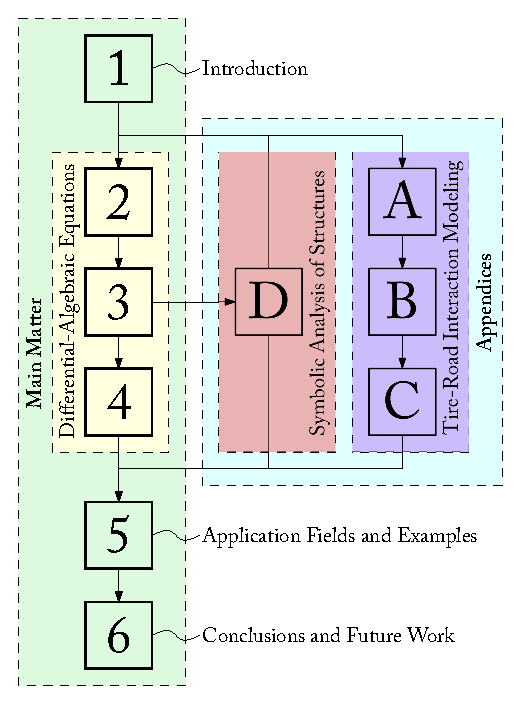
\includegraphics[width=9cm]{./figures/chapter_1/thesis_flowchart}
  \caption{Flowchart of the thesis structure, illustrating the logical progression of the chapters and appendices.}
  \label{chap1:fig:thesis_flowchart}
\end{figure}

% % % % % % % % % % % % % % % % % % % % % % % % % % % % % % % % % % % % % % % %

%!TEX root = ../main.tex

\chapter{Symbolic Computation and Applications}
\label{chapter:symbolic_computation}

Il calcolo simbolico è particolarmente utile per risolvere problemi che coinvolgono manipolazioni simboliche di espressioni matematiche piuttosto che semplici valori numerici. Ecco alcuni esempi di problemi in cui il calcolo simbolico si rivela prezioso:

Derivazione e Integrazione Simbolica:
Esempio 1: Calcolare la derivata di una funzione complessa, come ad esempio .
Esempio 2: Eseguire l'integrazione simbolica di una funzione come
Algebra Simbolica:
Esempio 3: Semplificare espressioni algebriche comple
Esempio 4: Risolvere sistemi di equazioni lineari o non lineari in forma simbolica.
Equazioni Differenziali Ordinarie (EDO):
Esempio 5: Risolvere un'equazione differenziale come
Esempio 6: Trovare una soluzione generale per un sistema di EDO complesso.
Matrici e Algebra Lineare:
Esempio 7: Calcolare l'inversa di una matrice simbolica.
Esempio 8: Trovare gli autovalori e gli autovettori di una matrice.
Teoria dei Numeri:
Esempio 9: Effettuare manipolazioni simboliche con espressioni che coinvolgono numeri irrazionali o complessi.
Esempio 10: Sviluppare algoritmi simbolici per la fattorizzazione di numeri o espressioni.


Chiarisco che l'analisi numerica solitamente coinvolge metodi computazionali basati su calcoli approssimati piuttosto che manipolazioni simboliche. Tuttavia, ci sono situazioni in cui il calcolo simbolico può essere incorporato nell'analisi numerica per migliorarne l'efficienza o risolvere specifici sotto-problemi. Ecco alcuni esempi:

Analisi di Errore:
Utilizzare il calcolo simbolico per derivare formule esatte per l'errore di approssimazione in un determinato metodo numerico, ad esempio, nell'approssimazione di una derivata o di un'integrale.
Ottimizzazione di Algoritmi Numerici:
Incorporare il calcolo simbolico per semplificare e ottimizzare passaggi critici in algoritmi numerici, ad esempio, nell'ottimizzazione di formule iterative o nella semplificazione di espressioni complesse all'interno di algoritmi.
Generazione di Funzioni Approssimanti:
Utilizzare il calcolo simbolico per derivare esattamente la forma chiusa di una funzione approssimante, ad esempio, attraverso metodi di interpolazione, semplificando così i calcoli numerici successivi.
Stabilità Numerica:
Analizzare la stabilità di un algoritmo numerico utilizzando il calcolo simbolico per esaminare il comportamento asintotico delle espressioni coinvolte nel processo numerico.
Risoluzione di Problemi Lineari o Non-Lineari:
Utilizzare tecniche di calcolo simbolico per semplificare le espressioni prima di applicare metodi numerici, riducendo così il numero di operazioni computazionali e migliorando l'efficienza computazionale.
Rappresentazione Esatta di Numeri Irrazionali:
Utilizzare il calcolo simbolico per rappresentare in modo esatto numeri irrazionali coinvolti in un problema numerico, evitando così errori di approssimazione.
Analisi di Sensibilità:
Utilizzare il calcolo simbolico per derivare espressioni analitiche per la sensibilità di una soluzione numerica rispetto alle variazioni nei parametri di input.
In queste situazioni, il calcolo simbolico può essere un complemento utile all'analisi numerica, contribuendo a una migliore comprensione del problema e ottimizzando l'implementazione degli algoritmi computazionali.
%!TEX root = ../main.tex

\chapter[DAEs Index Reduction and Numerical Solution]{Differential-Algebraic Equations Index Reduction and Numerical Solution}
\label{chap3:daes}

In this chapter, we present an algorithm for the index reduction of first-order \acp{DAE}. The proposed approach can be applied to generic \acp{DAE} and exploits neither a priori knowledge nor ad hoc techniques to leverage the specific formulation of the system. The index reduction is performed only by using symbolic manipulation and linear algebra techniques. It is based on the successive separation of the differential and algebraic equations of the system and the subsequent differentiation of the algebraic part. Improved symbolic matrix factorization is used to perform the \acp{DAE} partitioning, ensure numerical stability, and limit the expression swell of the reduced-index system. The effectiveness of the algorithm will be validated in the next chapter through a set of examples on a wide range of systems, including physical systems, engineering applications, and ``artificial'' \acp{DAE} with specific properties. The proposed symbolic index reduction algorithm is implemented in \Maple{} as part of an open-source library.

% % % % % % % % % % % % % % % % % % % % % % % % % % % % % % % % % % % % % % % %

\section{Differential-Algebraic Equations Index Reduction and Solution}
\label{chap3:sec:introduction}

As we already mentioned in Chapter~\ref{chap1:introduction}, \acp{DAE} are extensively used in dynamic system modeling. The challenge in numerically solving a \ac{DAE} system is assessed through its differentiation index, commonly referred to as ``the'' index~\cite{campbell1995index, campbell1995highindex}. Achieving accurate simulations necessitates converting high-index \acp{DAE} into low-index counterparts, posing a well-recognized challenge~\cite{petzold1982differential}. This process involves transforming a \ac{DAE} system into an equivalent system with a lower index through successive differentiation of the system equations. For this reason, the differentiation index is roughly defined as the number of times algebraic equations are differentiated to obtain an equivalent system of \acp{ODE} with invariants. Index reduction is a crucial step prior to the numerical integration of \acp{DAE}, as integrating high-index systems can be impractical. The primary obstacle lies in the necessity to solve non-linear systems of equations at each integration step, which can be computationally expensive and, in certain cases, numerically unstable. Specific numerical techniques, introduced in~\cite{petzold1982differential, thomsen1999numerical, baumgarte1972stabilization}, have been developed to address this challenge. However, these methods are not universally effective and may be inapplicable to some high-index \acp{DAE}. Consequently, index reduction becomes an indispensable preliminary stage before numerical integration~\cite{lamour2013differential}.

Given its complicated nature, index reduction has been the subject of extensive research and is often carried out by leveraging the specific formulation of the \ac{DAE} system, like in the multi-body modeling~\cite{zhou2005implicit, zhou2007symbolic, zhou2007symbolicseq, bayo1988modified, wehage1982generalized}. When the specific formulation of the \ac{DAE} system is not known a priori, or the system is not in a specific form, the index reduction process becomes more challenging. Many current simulation software packages for dynamic systems use index-reduction algorithms based on the \ac{SA} of the system, such as the Pantelides algorithm~\cite{pantelides1988consistent} and the dummy derivatives method~\cite{mattsson1993index}, which are subcases of the Pryce's $\Sigma$-method~\cite{pryce1998solving, pryce2001simple, nedialkov2007solvingI, nedialkov2007solvingII, nedialkov2008solvingIII, nedialkov2015algorithm, tan2016symbolic, mckenzie2017structural}. These algorithms are effective in reducing the index of most of the systems, but they can fail either for numerical cancellations~\cite{iwata2019index} or underestimation of the differentiation index~\cite{pantelides1988consistent, unger1995structural}, like in the case of Rei{\ss}ig's \acp{DAE} family~\cite{reissig2000differential}. Symbolic manipulation is proven to be successful in restating a \acp{DAE} on which the $\Sigma$-method fails to a \acp{DAE} on which the \ac{SA} may succeed~\cite{tan2016symbolic}.

Index reduction based on symbolic-numeric aided \ac{SA} has been successful in handling failures of the Pryce's $\Sigma$-method~\cite{tan2016symbolic} as well as in performing symbolically-informed \ac{SA}~\cite{chowdhry2004symbolic}. This latter \ac{SA} approach, which is named $\sigma v$-method, uses symbolic-numeric \ac{LU} factorization for variable substitution and rank determination on linear constant coefficient \acp{DAE}. A valuable attempt to use pure symbolic manipulation in \acp{DAE} index reduction is presented in~\cite{zhou2005implicit, zhou2007symbolic, zhou2007symbolicseq}, where implicit involutive form and \ac{LU} decomposition are successfully used to reduce the index of a simple constrained multi-body system. It is clear that index reduction algorithms based on pure symbolic matrix factorization represent a viable alternative to classic \ac{SA} techniques. However, symbolic matrix factorization feasibility is strongly tied to the performance of the symbolic computation kernel and its capabilities~\cite{zhou2008fraction}. Large expressions can lead to strong performance degradation of the kernel. Techniques aimed at limiting this decrease of performance while performing symbolic linear algebra operations are presented in~\cite{zhou2006hierarchical, zhou2007symbolic, zhou2007symbolicseq}. In these works, the hierarchical representation of expressions is applied to matrix factorization tasks. Nonetheless, the \LULEM{} package~\cite{carette2006linear}, which implements large expression management strategies in \ac{LU} decomposition, significantly outperforms the \Maple{}'s built-in matrix factorization routines.

The absence of user-invocable standalone functions within the \Maple{} environment that allows for the automatic index reduction of \acp{DAE}, and the inability to extract both the reduced-index system and invariants from the \texttt{dsolve} function, are the primary motivations of this research. Furthermore, recent advances in symbolic matrix factorization, combined with expressions hierarchical representation techniques, provide valuable tools that enable us to further investigate the applicability of a novel algorithm for the index reduction of \ac{DAE} systems, firstly presented in~\cite{stocco2024symbolic} as a preliminary work. The proposed methodology is similar to the previous work of~\citet{chowdhry2004symbolic} and extends it to generic first-order \acp{DAE}, linear in the states' derivatives. Nonetheless, the proposed algorithm does not work on the structural matrix of the system but on the \ac{DAE} system symbolic expressions. Specifically, the idea of using matrix factorization for variable substitution and rank determination is adopted to iteratively separate the differential and algebraic equations of the system. The algebraic equations are then differentiated to obtain an equivalent system with a lower differentiation index. Not less important, new libraries for symbolic matrix factorization (\LAST{}), large expression management (\LEM{}), and signature computation (\SIG{}) are presented. These libraries are based on the \LULEM{} package and extend the work of~\citet{zhou2006hierarchical, carette2006linear} and~\citet{zhou2007symbolic}. The newly presented libraries are designed to ensure the numerical stability of the numerically evaluated expressions, limit the expression swell, and provide an updated object-oriented interface. The effectiveness of the presented index reduction algorithm is validated through symbolic-numerical examples on a wide range of systems, including physical systems, engineering applications, as well as ``artificial'' systems with specific properties. The proposed algorithm is implemented in the \Maple{} environment and is available as a collection of open-source packages~\cite{last, lem}. Furthermore, the insights and the techniques presented in~\cite{zhou2006hierarchical, carette2006linear, zhou2007symbolic} are used to improve the presented algorithm to embed the hierarchical representation of expressions in a future implementation of the algorithm.

%This chapter is organized as follows. After this introduction (Section~\ref{chap3:sec:introduction}), the index reduction algorithm is presented in Section~\ref{chap3:sec:algorithm}. The expression swell mitigation, as well as the details on the symbolic matrix factorization, are discussed in Sections~\ref{chap3:sec:expression_swell} and \ref{chap3:sec:matrix_factorization}. The effectiveness of the algorithm is showcased through symbolic-numerical examples in Section~\ref{chap3:sec:example}. Finally, Sections~\ref{chap3:sec:future_work} and~\ref{chap3:sec:conclusions} report future developments and conclusions respectively. In~\ref{chap3:sec:cokernel} details on cokernel computation are reported. The newly developed object-oriented symbolic linear algebra (\ref{chap2:sec:last}), large expression management (\ref{chap2:sec:lem}) and signature computation (\ref{chap3:sec:signature}) package descriptions are also included in the appendices. The symbolic index reduction algorithm is implemented in the \Maple{} language and is available as part of the open-source \Indigo{} library~\cite{indigo}. Its usage is illustrated in~\ref{chap3:sec:index_reduction}.

% % % % % % % % % % % % % % % % % % % % % % % % % % % % % % % % % % % % % % % %

\section{A New Index Reduction Algorithm}
\label{chap3:sec:algorithm}

In this section, we explore the theoretical aspect of reducing the differential index of \ac{DAE} systems. Specifically, to systematically reduce the \ac{DAE} system's index, a novel iterative algorithm is presented. This algorithm comprises two main phases: initially, the separation of the differential equations from the algebraic equations inherent in \acp{DAE}; and subsequently, the differentiation of the algebraic ones to obtain an equivalent system with a reduced index. The algorithm that is presented in this section is implemented in the \Maple{} environment and is available as an open-source package~\cite{indigo}.

\subsection{Differential and Algebraic Equations Separation}
\label{chap3:sec:separation}

The initial phase of the index reduction procedure involves the partitioning of the \ac{DAE} system into its differential and algebraic equations. While in the case of small systems this can be accomplished through manual identification and isolation of the algebraic equations, this approach is inconvenient when dealing with large systems. An alternative method for automating the separation process leverages the cokernel, or left null space, of the \ac{DAE} system matrix, which is computed through matrix factorization techniques. The usage of the cokernel offers a more efficient and reliable means of accomplishing the separation task, variable substitution and not less importantly rank determination.

Consider a first-order system of \acp{DAE} $\mF$ of the form
%
\begin{equation}
  \label{chap3:eq:daes}
  \mF = \mA \, \mxp - \mb = \m{0}.
\end{equation}
%
We denote the cokernel and its orthogonal complement of $\mA$ with $\mK$ and $\mN$ respectively (see~\ref{chap3:sec:cokernel} for details on the cokernel computation with symbolic matrix factorization). Notice that the cokernel is the subspace obtained by the span of $\mK$'s columns. For this reason, hereafter, we refer to the cokernel as the matrix $\mK$ whose columns span the cokernel. Using $\mK$ and $\mN$ it is possible to separate the algebraic part of the \acp{DAE}~\eqref{chap3:eq:daes} as
%
\begin{equation}
  \label{chap3:eq:separated_daes}
  \begin{cases}
    \mE \, \mxp = \mg \\[0.1em]
    \ma = \m{0}
  \end{cases} \text{,} \quad \text{where} \qquad \mA = \begin{bmatrix}
    \mE \\[0.2em]
    \m{0}
  \end{bmatrix} \text{,}
  \quad \text{and} \quad
  \mb = \begin{bmatrix}
     \mg \\[0.2em]
     \ma
  \end{bmatrix} \text{.}
\end{equation}
%
The separated equations of the \acp{DAE} are obtained by the left product of $\mK$ and $\mN$ as
%
\begin{equation}
  \begin{array}{l@{~}c@{~}l}
    \mE &=& \mN \, \mA \text{,} \\[0.1em]
    \mg &=& \mN \, \mb \text{,} \\[0.1em]
    \ma &=& \mK \, \mb \text{.}
  \end{array}
\end{equation}
%
This results in an equivalent \ac{DAE} system, where the algebraic equations $\ma$ are now explicit. The details of the cokernel and its orthogonal complement computation are discussed in~\ref{chap3:sec:cokernel}.


\subsubsection{Cokernel Computation with Matrix Factorization}
\label{chap3:sec:cokernel}

The cokernel of a generic matrix $\m{A}$ is denoted as $\m{K}$ and satisfy $\m{K}\m{A} = \m{0}$. As mentioned before, the cokernel is the subspace obtained by the span of $\m{K}$'s columns. The orthogonal complement of the cokernel is denoted as $\m{N}$, moreover, the matrices $\m{N}$ and $\m{K}$ stacked compose a square non-singular matrix. It is common knowledge that matrix factorization techniques can be employed to compute the cokernel and its orthogonal complement. Among these techniques, the \ac{LU} factorization stands out as one of the most frequently used methods.

\paragraph{Lower-Upper Decomposition}

The full-pivoting \ac{LU} decomposition of a matrix $\m{A} \in \mathbb{R}^{m \times n}$ (with $m\geq n$) is represented as the product of matrices $\m{L}$ and $\m{U}$ with the permutation matrices $\mP$ and $\mQ$. It is characterized by the following properties:
%
\begin{itemize}
  \setlength{\itemsep}{0.0em}
  \item $\mP\m{A}\mQ = \m{L}\m{U}$;
  \item $\m{L} \in \mathbb{R}^{m \times m}$ is a lower-triangular matrix with all diagonal entries equal to $1$;
  \item $\m{U} \in \mathbb{R}^{m \times n}$ is an upper-triangular matrix;
  \item $\mP \in \mathbb{R}^{m \times m}$ and $\mQ \in \mathbb{R}^{n \times n}$ are the rows and columns permutation matrices, respectively.
\end{itemize}
%
If $\m{M}$ is defined such that $\m{M} = \m{L}^{-1}\mP$, then the following relation holds
%
\begin{equation}
    \m{M}\m{A}
    = \m{L}^{-1}\mP\m{A}
    = \m{L}^{-1}\mP\m{A}\mQ\mQ^\top
    = \m{L}^{-1}\m{L}\m{U}\mQ^\top
    = \m{U}\mQ^\top
    = \begin{bmatrix} \m{U}_1 \\[0.2em] \m{0} \end{bmatrix}\mQ^\top \text{.}
\end{equation}
%
If the identity matrix $\mI$ is partitioned as
%
\begin{equation}
  \mI = \begin{bmatrix}
    \mI_1 & \m{0} \\[0.2em]
    \m{0} & \mI_2
  \end{bmatrix} \text{,}
  %
  \quad \text{where} \quad
  %
  \begin{array}{l}
    \mI_1 \in \mathbb{R}^{m \times m} \quad \text{and} \quad
    \mI_2 \in \mathbb{R}^{(m-n)\times(m-n)}\text{,}
  \end{array}
\end{equation}
%
we can write
%
\begin{equation}
  \begin{bmatrix} \mI_1 & \m{0} \end{bmatrix} \, \m{M}\m{A} =
  \begin{bmatrix} \mI_1 & \m{0} \end{bmatrix}
  \begin{bmatrix} \m{U}_1 \\[0.2em] \m{0} \end{bmatrix} \mQ^\top = \m{U}_1 \mQ^\top
  %
  , \qquad \text{and} \qquad
  %
  \begin{bmatrix} \m{0} & \mI_2 \end{bmatrix} \, \m{M}\m{A} =
  \begin{bmatrix} \m{0} & \mI_2 \end{bmatrix}
  \begin{bmatrix} \m{U}_2 \\[0.2em] \m{0} \end{bmatrix} \mQ^\top = \m{0} \text{.}
\end{equation}
%
Eventually, the matrices $\m{N}$ and $\m{K}$ have the following form
%
\begin{equation*}
  \m{N} = \begin{bmatrix} \mI_1 & \m{0} \end{bmatrix} \, \m{M}
  %
  \quad \text{and} \quad
  %
  \m{K} = \begin{bmatrix} \m{0} & \mI_2 \end{bmatrix} \, \m{M},
\end{equation*}
%
where
%
\begin{equation*}
  \begin{array}{l}
      \m{K}\m{A} = \m{0} \\[0.2em]
      \m{N}\m{A} = \m{U}_1 ~ \text{is full-rank}
  \end{array} \, \text{,}
  %
  \quad \text{and} \quad
  %
  \begin{bmatrix} \m{N} \\[0.2em] \m{K} \end{bmatrix} \quad \text{is non-singular.}
\end{equation*}

\paragraph{Fraction-Free Lower-Upper Decomposition}

The \ac{FFLU} factorization is a variant of the \ac{LU} decomposition. It is based on the same principles as the standard \ac{LU} decomposition, but it is designed to avoid the appearance of fractions in the intermediate results. Similarly to the \ac{LU} case, the \ac{FFLU} decomposition of a matrix $\m{A} \in \mathbb{R}^{m \times n}$ (with $m\geq n$) is represented as the quintet of matrices $\m{L}$, $\m{U}$, $\m{D}$, $\mP$, and $\mQ$, and is characterized by the properties:
%
\begin{itemize}
  \setlength{\itemsep}{0.0em}
  \item $\mP\m{D}\m{A}\mQ = \m{L}\m{U}$;
  \item $\m{L} \in \mathbb{R}^{m \times m}$ is a lower-triangular matrix with all diagonal entries equal to $1$;
  \item $\m{D} \in \mathbb{R}^{m \times m}$ is a diagonal matrix;
  \item $\m{U} \in \mathbb{R}^{m \times n}$ is an upper-triangular matrix;
  \item $\mP \in \mathbb{R}^{m \times m}$ and $\mQ \in \mathbb{R}^{n \times n}$ are the rows and columns permutation matrices, respectively.
\end{itemize}
%
The procedure for computing the cokernel of a matrix $\m{A}$ using the \ac{FFLU} is similar to the case of the \ac{LU} decomposition. The only difference is in the computation of the matrix product $\m{M}\m{A}$. If $\m{M} = \m{L}^{-1}\mP\m{D}$, then $\m{M}\m{A}$ are written as
%
\begin{equation}
  \m{M}\m{A}
  = \m{L}^{-1}\mP\m{D}\m{A}
  = \m{L}^{-1}\mP\m{D}\m{A}\mQ\mQ^\top
  = \m{L}^{-1}\m{L}\m{U}\mQ^\top
  = \m{U}\mQ^\top = \begin{bmatrix} \m{U}_1 \\[0.2em] \m{0} \end{bmatrix}\mQ^\top \text{.}
\end{equation}
%
Then, the subspaces $\m{N}$ and $\m{K}$ are computed as in the \ac{LU} case.

\subsection{Algebraic Equations Differentiation}
\label{chap3:sec:differentiation}

The algebraic equations in the \ac{DAE} system~\eqref{chap3:eq:separated_daes} are now differentiated as
%
\begin{equation}
  \label{chap3:eq:diff_daes}
  \dfrac{\mathrm{d}}{\mathrm{d}t} \ma = \mAd \, \mxp - \mgd \text{.}
\end{equation}
%
The \acp{DAE}~\eqref{chap3:eq:separated_daes} after differentiation of algebraic equations now take a form similar to that of~\eqref{chap3:eq:daes}, where
%
\begin{equation}
  \label{chap3:eq:reduced_daes}
  \mA = \begin{bmatrix} \mE \\[0.2em] \mAd\end{bmatrix} \text{,}
  \quad \text{and} \quad
  \mb = \begin{bmatrix} \mg \\[0.2em] \mgd\end{bmatrix} \text{.}
\end{equation}
%
The set of invariants, which are collected in $\mh$, is updated adding the algebraic equations $\ma$
%
\begin{equation}
  \mh \quad \xleftarrow[\text{update}]{\text{\, Invariants \,}} \quad \overset{{\text{The old $\mh$}}}{\begin{bmatrix} \overbrace{\mh} \\[0.2em] \ma \end{bmatrix}} \text{.}
\end{equation}
%
The iterative procedure, involving the sequential separation and differentiation of the algebraic segment of the system, is iterated until $\mA$ is non-singular. When $\mA$ is non-singular the \ac{DAE} corresponds to a system of \acp{ODE} compounded by the invariants $\mh$, which are the collection of the hidden constraints produced in the index reduction process. The invariants $\mh$ can be initialized empty or with user-defined algebraic equations aimed at preserving crucial system properties, such as energy conservation and/or momentum conservation. A pseudocode of the index reduction algorithm can be found in Algorithm~\ref{chap3:alg:index_reduction}.

\begin{breakablealgorithm}
  \caption{Index reduction algorithm (without large expression management)~\cite{stocco2024symbolic}.}
  \label{chap3:alg:index_reduction}
  \begin{algorithmic}[1]
    \State \textbf{Require:} A \ac{DAE} system of the form $\mF \eqdef \mA \, \mxp - \mb = \m{0}$.
    \Procedure{ReduceIndex}{$\mF$} \Comment{Index reduction procedure}
      \State $\mh \gets \varnothing$ \Comment{The set of invariants}
      \State $\mA, \, \mb \gets \mathrm{GenerateMatrix}(\mF, \, \mxp)$ \Comment{The \ac{DAE} system matrix}
      \State $m \gets \mathrm{Size}(\mx)$\Comment{The size of $\mx$}
      \While{$\mA$ is singular}
        \State $\displaystyle\triangleright$ Differential and algebraic equations separation (Section~\ref{chap3:sec:separation})
        \State $\mL, \, \mU, \, \mP, \, \mQ \gets \mathrm{MatrixFactorization}(\mA)$ \Comment{LU or FFLU decomposition of $\mA$}
        \State $r \gets \mathrm{Rank}(\mU)$ \Comment{The rank of $\mU$ is equal to the rank of $\mA$}
        \State $\mI_1 \gets \mathrm{IdentityMatrix}(r, \, r)$ \Comment{The upper identity matrix}
        \State $\mI_2 \gets \mathrm{IdentityMatrix}(m-r, \, m-r)$ \Comment{The lower identity matrix}
        \State $\mE \gets \begin{bmatrix} \mI_1, \, \m{0} \end{bmatrix} \, \mU \, \mQ^\top$ \Comment{The reordered part of $\mA$}
        \State $\mg \gets \begin{bmatrix} \mI_1, \, \m{0} \end{bmatrix} \, \mL^{-1} \, \mP \, \mb$ \Comment{The differential part of $\mb$}
        \State $\ma \gets \begin{bmatrix} \m{0}, \, \mI_2 \end{bmatrix} \, \mL^{-1} \, \mP \, \mb$ \Comment{The algebraic part of $\mb$}
        \State $\displaystyle\triangleright$ Algebraic equations differentiation (Section~\ref{chap3:sec:differentiation})
        \State $\mAd, \, \mgd \gets \mathrm{GenerateMatrix}(\mathrm{Diff}(\ma, \, t), \, \mxp)$ \Comment{Differentiate the equations $\ma$}
        \State $\mA \gets \begin{bmatrix} \mE \\ \mAd \end{bmatrix}$ and $\mb \gets \begin{bmatrix} \mg \\ \mgd \end{bmatrix}$
        \Comment{The new matrix $\mA$ and vector $\mb$}
        \State $\mh \gets \mh \cup \ma$ \Comment{Add the algebraic equations to the set of invariants}
      \EndWhile \\
      \Return $\mA, \, \mb, \, \mh$ \Comment{The \acp{DAE} reduced to an \ac{ODE} system with invariants}
    \EndProcedure
  \end{algorithmic}
\end{breakablealgorithm}

\subsection{A Step-by-Step Example}
\label{chap3:sec:step_by_step}

Within this Section, we present the step-by-step results of the index reduction algorithm. To do so we exploit a simple non-stiff index-3 problem found in \Wolfram{}~\Mathematica{} documentation~\cite{mathematica}. The initial value problem is defined as follows
%
\begin{equation}
  \label{chap3:eq:index_3}
  \mF = \begin{bmatrix}
    x^{\prime}_{2} - x_{1} - \cos(t) \\
    x^{\prime}_{3} - x_{2} - \sin(t) \\
    x_{3} - \cos(t)
  \end{bmatrix},
\end{equation}
%
with states $\mx = [x_{1}, \, x_{2}, \, x_{3}]^\top$ and initial conditions $\mx_{0} = [-1, \, 0, \, 1]^\top$. Notice that the analytical solution of this problem is $\mx_\text{exact} = [\sin(t) - 2\cos(t), \, 2\sin(t), \, \cos(t)]^\top$. The index reduction algorithm is applied to the \ac{DAE} system~\eqref{chap3:eq:index_3} and the step-by-step results for the matrices $\mE$, $\mg$, and $\ma$ are reported here below.
%
\begin{equation*}
  \begin{array}{l}
    \text{Index-3 \acp{DAE}:} \quad \mE = \begin{bmatrix}
      0 & 1 & 0 \\
      0 & 0 & 1
    \end{bmatrix}, \quad
    \mg = \begin{bmatrix}
      \sin(t) - x_{1} \\
      \sin(t) - x_{2}
    \end{bmatrix}, \quad
    \ma = \begin{bmatrix}
      \cos(t) - x_{3}
    \end{bmatrix}. \\[1.0em]
    %
    \text{Index-2 \acp{DAE}:} \quad \mE = \begin{bmatrix}
      0 & 1 & 0 \\
      0 & 0 & 1
    \end{bmatrix}, \quad
    \mg = \begin{bmatrix}
      \sin(t) - x_{1} \\
      \sin(t) - x_{2}
    \end{bmatrix}, \quad
    \ma = \begin{bmatrix}
      2\sin(t) - x_{2}
    \end{bmatrix}. \\[1.0em]
    %
    \text{Index-1 \acp{DAE}:} \quad \mE = \begin{bmatrix}
      0 & 0 & 1 \\
      0 & 1 & 0
    \end{bmatrix}, \quad
    \mg = \begin{bmatrix}
      \sin(t) - x_{2} \\
      \sin(t) - x_{1}
    \end{bmatrix}, \quad
    \ma = \begin{bmatrix}
      \sin(t) - 2\cos(t) - x_{1}
    \end{bmatrix}. \\[1.0em]
    %
    \text{Index-0 \acp{DAE}:} \quad \mE = \begin{bmatrix}
      0 & 0 & 1 \\
      0 & 1 & 0 \\
      1 & 0 & 0
    \end{bmatrix}, \quad
    \mg = \begin{bmatrix}
      \sin(t) - x_{2} \\
      \sin(t) - x_{1} \\
      2\sin(t) + \cos(t)
    \end{bmatrix}, \quad
    \ma = \varnothing.
  \end{array}
\end{equation*}
%
The final form of the system is an index-0 \acp{DAE} system is then
%
\begin{equation}
  \label{chap3:eq:index_3_reduced}
  \mF = \begin{bmatrix}
    x^{\prime}_{2} - x_{1} - \cos(t) \\
    x^{\prime}_{3} - x_{2} - \sin(t) \\
    x^{\prime}_{1} - \cos(t) - 2\sin(t)
  \end{bmatrix},
  %
  \quad \text{with invariants} \quad
  %
  \mh = \begin{bmatrix}
    \cos(t) - x_{3} \\
    2\sin(t) - x_{2} \\
    \sin(t) - 2\cos(t) - x_{1}
  \end{bmatrix}.
\end{equation}
%
Although the just presented example is not so complex and relevant for a real validation of the algorithm, it is useful to demonstrate the step-by-step results of the index reduction algorithm. Furthermore, the expression complexities encountered throughout the index reduction algorithm applied to the Index-3 problem are reported below in \tablename{}~\ref{chap3:tab:index_3}.

\begin{table}
  \caption{Expression complexity encountered throughout the index reduction of the index-3 step-by-step example problem~\cite{mathematica} \ac{DAE} system index reduction. \emph{Legend}: $\cf$ = functions, $\ca$ = additions, $\cm$ = multiplications, and $\cd$ = divisions.}
  \label{chap3:tab:index_3}
  \centering
  {\footnotesize\begin{tabular}{cccc}
    \multicolumn{4}{c}{\textbf{Index-3 \acp{DAE}~\cite{mathematica}}} \\
    \toprule
    \textbf{Original \acp{DAE}} & \multicolumn{3}{c}{$\mF = 10\cf + 5\ca$ \quad $\mh = 0$} \\
    \midrule
    \textbf{Reduction step} & $\mE$ & $\mg$ & $\ma$ \\
    \midrule
    Index-3 \acp{DAE} & $0$ & $4\cf + 2\ca$ & $2\cf + 1\ca$ \\
    Index-2 \acp{DAE} & $0$ & $4\cf + 2\ca$ & $2\cf + 1\cm + 1\ca$ \\
    Index-1 \acp{DAE} & $0$ & $4\cf + 2\ca$ & $3\cf + 1\cm + 1\ca$ \\
    Index-0 \acp{DAE} & $0$ & $6\cf + 1\cm + 3\ca$ & $0$ \\
    \midrule
    \textbf{Reduced \acp{DAE}} & \multicolumn{3}{c}{$\mF = 12\cf + 1\cm + 6\ca$ \quad $\mh = 7\cf + 2\cm + 4\ca$} \\
    \bottomrule
    \end{tabular}}
\end{table}

\subsection{Acknowledging some Algorithm Limitations}

While the algorithm just presented is relatively straightforward to implement, it does have two major sources of potential issues that are both determined by the technology used and the fundamental theory.
%
\begin{itemize}
    \item \emph{Expression complexity}. Symbolic manipulation often leads to a growth in expression complexity. For this reason, expression simplification may not always be feasible due to software limitations or excessive CPU time demands. Making the algorithm insensitive to expression swell is thus crucial to its effectiveness.
    \item \emph{Numerical stability of symbolic matrix factorization}. The description of the algorithm involves the manipulation of matrices and vectors with either symbolic or mixed symbolic-numeric entries. Ensuring that symbolic matrix factorization maintains numerical stability is a critical requirement of the algorithm. In the case of \ac{LU} decomposition, inadequate pivoting strategies can lead to the generation of singular matrices, which in turn can cause the algorithm to fail~\cite{zhou2005implicit, zhou2007symbolic, giesbrecht2014symbolic}.
\end{itemize}
%
These are the two main points that we acknowledge in the implementation of the algorithm. In the forthcoming sections, each of these matters is discussed in detail, with recommendations on techniques and open-source software solutions that are used to address them.

\section{Index Reduction Algorithm with Expression Swell Mitigation}

The most interesting and relevant aspect to be explored is the connection between the hierarchical representation of expressions (see Section~\ref{chap2:sec:lem}) and the \ac{DAE} index reduction. The use of veiling variables may be used to hide some parts of the expressions by the collection of common sub-expressions. Even if this may appear to be a substantial improvement, it is not so frequent to encounter expressions that are common to all the equations of the \ac{DAE} system. Still, this concept can be extended to mitigate the expression swell during matrix factorization (see Section~\ref{chap2:sec:last}). The veiling variables $\mv$ would then include the states $\mx$ of the \ac{DAE} system. In this manner, the hierarchical representation of the expression serves as a system augmentation technique as well as a means to limit expression swell during the index reduction procedure. The augmented \ac{DAE} system would then be expressed as
%
\begin{equation}
  \label{chap3:eq:augmented_dae}
  \mFv = \mAv \, \mx^\prime - \mbv = \m{0},
  %
  \qquad \text{where} \qquad
  %
  \mv = \begin{bmatrix}
    v_{1}(\mx, t) \\
    v_{2}(v_{1}, \mx, t) \\
    \vdots \\
    v_{n}(v_{1}, \dots, v_{n-1}, \mx, t) \\
  \end{bmatrix}.
\end{equation}
%
Notice that if the matrix $\mAv$ is non-singular, the augmented \ac{DAE} system~\eqref{chap3:eq:augmented_dae} has index-1. This is a crucial aspect to be taken into consideration since, as demonstrated in Section~\ref{chap3:sec:daes_complexity}, the final reduction to index-0 \acp{DAE} is costly. Furthermore, the vector $\mv$ and its Jacobian with respect to the states $\mx$ can be sequentially evaluated for additional reduction of the computational burden. Nonetheless, the augmented formulation~\eqref{chap3:eq:augmented_dae} allows for the full exploitation of the signature technique to detect null expressions without the need for symbolic simplification~\cite{monagan1994signature}. Eventually, this will be the subject of future research and implementations that will exploit index-1 \acp{DAE} integrators similarly to the other state-of-the-art \acp{DAE} solver presented in the Introduction. A pseudocode and a flowchart of the index reduction algorithm with expression swell mitigation can be found in Algorithm~\ref{chap3:alg:index_reduction_veil} and \figurename~\ref{chap3:fig:index_reduction_veil}, respectively.

\begin{figure}[htp]
  \centering
  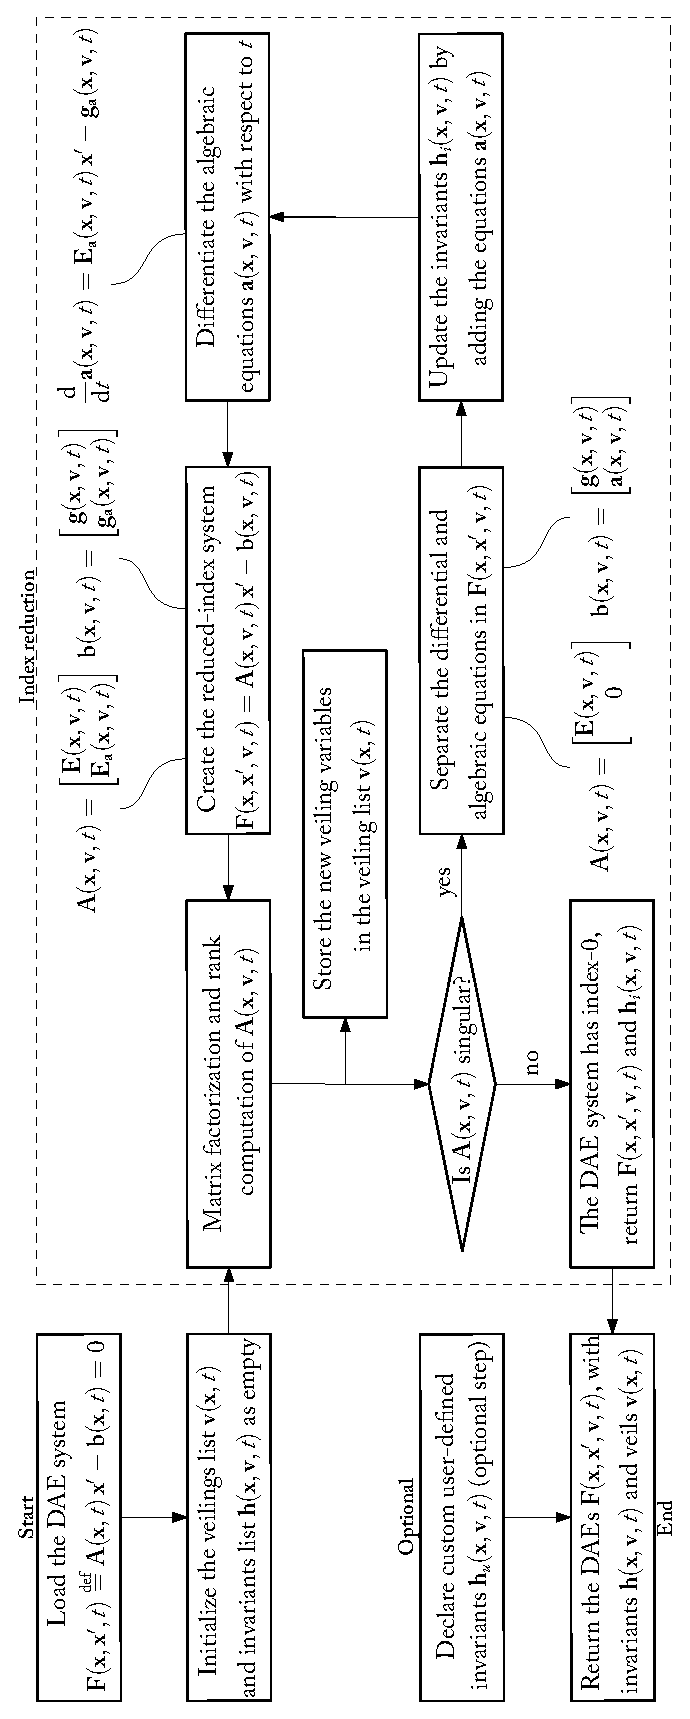
\includegraphics[angle=0, width=0.5\columnwidth]{dae_flowchart_veil}
  \caption{Flowchart of the index reduction algorithm with expression swell mitigation.}
  \label{chap3:fig:index_reduction_veil}
\end{figure}

\begin{breakablealgorithm}
  \caption{Index reduction algorithm with expression swell mitigation.}
  \label{chap3:alg:index_reduction_veil}
  \begin{algorithmic}[1]
    \State \textbf{Require:} A \ac{DAE} system of the form $\mFv \eqdef \mAv \, \mxp - \mbv = \m{0}$.
    \Procedure{ReduceIndex}{$\mFv$} \Comment{Index reduction procedure}
      \State $\mhiv \gets \varnothing$ \Comment{The set of invariants}
      \State $\mv \gets \varnothing$ \Comment{The veiling variables vector}
      \State $\mAv, \, \mbv \gets \mathrm{GenerateMatrix}(\mFv, \, \mxp)$ \Comment{The \ac{DAE} system matrix}
      \State $m \gets \mathrm{Size}(\mx)$\Comment{The size of $\mx$}
      \While{$\mAv$ is singular}
        \State $\displaystyle\triangleright$ Differential and algebraic equations separation (Section~\ref{chap3:sec:separation})
        \State $\mLv, \, \mUv, \, \mP, \, \mQ, \, \m{v}_d(\mx, \m{v}, \, t) \gets \mathrm{MatrixFactorization}(\mAv)$ \Comment{\ac{LU} or \ac{FFLU} decomposition of $\mAv$ with new veiling variables $\m{v}_d(\mx, \m{v}, \, t)$}
        \State $\mv \gets \mv \cup \m{v}_d(\mx, \m{v}, \, t)$ \Comment{Update the veiling variables vector}
        \State $r \gets \mathrm{Rank}(\mUv)$ \Comment{The rank of $\mUv$ is equal to the rank of $\mAv$}
        \State $\mI_1 \gets \mathrm{IdentityMatrix}(r, \, r)$ \Comment{The upper identity matrix}
        \State $\mI_2 \gets \mathrm{IdentityMatrix}(m-r, \, m-r)$ \Comment{The lower identity matrix}
        \State $\mEv \gets \begin{bmatrix} \mI_1, \, \m{0} \end{bmatrix} \, \mUv \, \mQ^\top$ \Comment{The reordered part of $\mAv$}
        \State $\mgv \gets \begin{bmatrix} \mI_1, \, \m{0} \end{bmatrix} \, \mLv^{-1} \, \mP \, \mbv$ \Comment{The differential part of $\mbv$}
        \State $\mav \gets \begin{bmatrix} \m{0}, \, \mI_2 \end{bmatrix} \, \mLv^{-1} \, \mP \, \mbv$ \Comment{The algebraic part of $\mbv$}
        \State $\displaystyle\triangleright$ Algebraic equations differentiation (Section~\ref{chap3:sec:differentiation})
        \State $\jac{\m{v}}{\mx}(\mx, \m{v}, \, t) \gets \mathrm{Jacobian}(\mv, \, \mx)$ \Comment{The Jacobian of $\mav$ with respect to $\mx$}
        \State $\mav \gets \mathrm{Diff}(\mav, \, t)$ \Comment{Differentiate the equations $\mav$}
        \State $\mav \gets \mathrm{Substitute}(\jac{\m{v}}{\mx}(\mx, \m{v}, \, t), \mav)$ \Comment{Remove the $\mv$ derivatives from $\mav$}
        \State $\mAdv, \, \mgdv \gets \mathrm{GenerateMatrix}(\mav, \, \mxp)$ \Comment{Differentiate the equations $\mav$}
        \State $\mAv \gets \begin{bmatrix} \mEv \\ \mAdv \end{bmatrix}$ and $\mbv \gets \begin{bmatrix} \mgv \\ \mgdv \end{bmatrix}$
        \Comment{The new matrix $\mAv$ and vector $\mbv$}
        \State $\mhiv \gets \mhiv \cup \mav$ \Comment{Add the algebraic equations to the set of invariants}
      \EndWhile \\
      \Return $\mAv, \, \mbv, \, \mhiv, \, \mv$ \Comment{The \acp{DAE} reduced to an \ac{ODE} system with invariants}
    \EndProcedure
  \end{algorithmic}
\end{breakablealgorithm}

% % % % % % % % % % % % % % % % % % % % % % % % % % % % % % % % % % % % % % % %

\section{Index Reduction and Numerical Integration Scheme}
\label{chap3:sec:indigo}

After this fairly long discussion on the actual implementation aspects of the index reduction algorithm, we can now present the \Indigo{} index reduction and integration toolbox~\cite{indigo}. This toolbox consists of two main components: a \Maple{} package to carry out symbolic index reduction of \ac{DAE} systems, and a \Matlab{} toolbox to perform numerical integration of the reduced-index system. \Indigo{} is designed to be used in conjunction with the \LEM{} package, to limit the expression swell, and the \LAST{} package, to conveniently factorize matrices. In the following paragraphs, we briefly discuss the usage of the \Indigo{} package.

\subsection{Index Reduction}

The index reduction algorithm implemented in the \Indigo{} \Maple{} package is the one presented in Section~\ref{chap3:sec:algorithm}. To reduce the index of a \ac{DAE} system in the \Maple{} environment we need to first create an \Indigo{} object instance.
%
\begin{verbatim}
> Indigo_obj := Object(Indigo);
> Indigo_obj:-InitLAST();
\end{verbatim}
%
Then, the system of \acp{DAE} \texttt{eqns} with coordinates \texttt{vars} is loaded.
%
\begin{verbatim}
> Indigo_obj:-LoadEquations('Generic', eqns, vars);
\end{verbatim}
%
The \texttt{Generic} symbol is used to specify the type of the system. Notice that in this example, we assume that the equations of the system are already available in the \Maple{} session. The automatic index reduction process can be performed by calling the \texttt{ReduceIndex} method, which iterates the separation and differentiation steps until an index-$0$ \ac{DAE} system is obtained.
%
\begin{verbatim}
> Indigo_obj:-ReduceIndex();
\end{verbatim}
%
Intermediate results of the process are stored internally in the \Indigo{} object and are available on demand. Once the index reduction process is completed, the user can generate the \texttt{SliderCrank} \Matlab{} class file to perform numerical integration of the reduced-index system.
%
\begin{verbatim}
> Indigo_obj:-GenerateMatlabCode(name, type, data=pars);
\end{verbatim}
%
A file \texttt{name.m} is generated in the current directory. As it is explained in the next section, The string parameter \texttt{type} can be either \texttt{Implicit}, \texttt{SemiExplicit} or \texttt{Explicit} depending on the desired numerical integration scheme. The optional parameter \texttt{data} introduces default internal object data.

\subsection{Numerical Integration Scheme}

The \Indigo{} \Matlab{} toolbox is an object-oriented library that allows the user to exploit the automatically generated code of the reduced-index system. It is capable of integrating systems of \acp{ODE} and \acp{DAE} using a variety of Runge-Kutta numerical integration schemes. In particular, the system of equations which is integrated is composed of the following elements.
%
\begin{itemize}
  \setlength{\itemsep}{0pt}
    \item A differential part, which can be expressed by one of the following classes:
    %
    \begin{equation}
        \begin{array}{ccl}
            \m{F}(\mx, \mx^\prime, \m{v}, t) = \m{0} & \hspace{0.5cm} &
            \text{\texttt{Implicit} system class,} \\[0.5mm]
            \m{A}(\mx, \m{v}, t) \, \mx^\prime = \m{b}(\mx, \m{v}, t) & \hspace{0.5cm} &
            \text{\texttt{SemiExplicit} system class,} \\[0.5mm]
            \mx^\prime = \m{f}(\mx, \m{v}, t) & \hspace{0.5cm} &
            \text{\texttt{Explicit} system class.}
        \end{array}
    \end{equation}
    %
    \item The invariants, composed of the hidden constraints obtained from the index reduction process $\mhiv$, and optional user-defined invariants $\mhuv$, namely
    %
    \begin{equation}
        \label{chap3:eq:inv_part}
        \m{h}(\mx, \m{v}, t) = \begin{bmatrix}
            \mhiv \\[0.5mm]
            \mhuv
        \end{bmatrix} = \m{0} \text{.}
    \end{equation}
    %
    \item The veils, which are the set of the expression hierarchical representation variables used in \LEM{} to limit the expression swell
    %
    \begin{equation}
        \m{v}(\mx, t) = \begin{bmatrix}
            v_{1}(\mx, t) \\[0.5mm]
            v_{2}(v_{1}, \mx, t) \\
            \vdots \\
            v_{n}(v_{1}, \dots, v_{n-1}, \mx, t)
        \end{bmatrix} \text{.}
    \end{equation}
\end{itemize}

To respect the invariants during the integration the \emph{standard projection} method is applied~\cite{hairer2000symmetric}. This method consists of projecting the solution $\mx$ of the numerically integrated reduced-index system onto the invariants manifold $\m{h}(\mx, \m{v}, t) = \m{0}$, which is equivalent to the following constrained minimization
%
\begin{equation}
  \underset{\widetilde{\mx}}{\textrm{minimize}} \quad \dfrac{1}{2}\left(\mx - \widetilde{\mx}\right)^2
    \quad \textrm{subject to} \quad
    \m{h}(\mx, \m{v}, t) = \m{0}.
\end{equation}

To integrate the system generated through the \Matlab{} package or a custom system \texttt{sys}, the user must first instantiate a \Indigo{} Runge-Kutta solver.
%
\begin{verbatim}
>>> solver = IndigoSolver('solver_name');
>>> solver.set_system(sys);
\end{verbatim}
%
Once the solver is instantiated, it is only necessary to specify the initial conditions and the integration time vector.
%
\begin{verbatim}
>>> [x, t, v, h] = solver.solve(t_ini:d_t:t_end, ics);
\end{verbatim}
%
The solver returns the solution of the system in the form of multiple outputs: \texttt{x} contains the integrated solution, \texttt{x\_dot} the states' time derivative, \texttt{t} the time vector, \texttt{v} the veiling variables, and finally \texttt{h} the values of the invariants over the specified time mesh \texttt{t\_ini:d\_t:t\_end}.

% % % % % % % % % % % % % % % % % % % % % % % % % % % % % % % % % % % % % % % %

\section{Proofing the Symbolic-Numeric Scheme}
\label{chap3:sec:example}

In this section, we showcase an example of a high-index \ac{DAE} system: an index-3 problem with an analytical solution, which describes the motion of a particle on a 3D torus surface~\cite{campbell1995constraint}. This example is employed to validate the numerical stability of the reduced-index system, as well as the good conditioning of both the symbolic matrix factorization and the numerical integration scheme. To ease the understanding of the results, we purposely avoid the use of the veiling variables in this example. However, the veiling variables just add an evaluation layer to the expressions, and they do not affect the numerical stability of the algorithm.

\subsection{Expression Complexity of the Reduced-Index Systems}
\label{chap3:sec:daes_complexity}

As a first demonstration of the proposed index reduction algorithm capabilities, we first consider the given example from a purely symbolic perspective. In particular, we consider the computational cost of the expressions generated during the presented procedure. The compactness of the expressions generated during the index reduction algorithm is a crucial aspect, as it ensures that limited computational overhead is introduced in the numerical integration of the reduced-index system, as well as in the projection of the solution on the hidden constraints. Specifically, the index reduction algorithm is applied to the \ac{DAE} system and reduced to index-0. For each reduction stage of the example considered, the computational cost is reported in \tablename{}~\ref{chap3:tab:torus}.

\begin{table}[htp]
  \caption{Expression complexity encountered throughout the index reduction of the robotic arm problem~\cite{brenan1995numerical} \ac{DAE} system index reduction. \emph{Legend}: $\cf$ = functions, $\ca$ = additions, $\cm$ = multiplications, and $\cd$ = divisions.}
  \label{chap3:tab:torus}
  \centering
  {\footnotesize\begin{tabular}{cccc}
    \multicolumn{4}{c}{\textbf{Particle Motion~\cite{campbell1995constraint}}} \\
    \toprule
    \textbf{Original \acp{DAE}} & \multicolumn{3}{c}{$\mF = 47\cf + 30\cm + 23\ca$ \quad $\mh = 0$} \\
    \midrule
    \textbf{Reduction step} & $\mE$ & $\mg$ & $\ma$ \\
    \midrule
    Index-3 \acp{DAE} & $0$ & $39\cf + 36\cm + 13\ca$ & $7\cf + 10\cm + 6\ca$ \\
    Index-2 \acp{DAE} & $0$ & $39\cf + 36\cm + 13\ca$ & $22\cf + 20\cm + 8\ca$ \\
    Index-1 \acp{DAE} & $0$ & $39\cf + 36\cm + 13\ca$ & $68\cf + 72\cm + 33\ca$ \\
    Index-0 \acp{DAE} & $388\cf + 424\cm + 180\ca$ & $79\cf + 77\cm + 26\ca$ & $0$ \\
    \midrule
    \textbf{Reduced \acp{DAE}} & \multicolumn{3}{c}{$\mF = 258\cf + 239\cm + 109\ca$ \quad $\mh = 97\cf + 102\cm + 47\ca$} \\
    \bottomrule
    \end{tabular}}
\end{table}

\subsection{Numerical Integration of the Reduced-Index System}
\label{chap3:sec:numerical_integration}

The numerical stability and consistency of the reduced-index system are demonstrated by exploiting the analytical solution of the problem in~\cite{campbell1995constraint}. Specifically, the \ac{DAE} system consists of three position variables $[x_{1}, \, x_{2}, \, x_{3}]^\top$, three velocity variables $[u_{1}, \, u_{2}, \, u_{3}]^\top$, and one constraint with Lagrange multiplier $\lambda$. The solution manifold is 4D, and the exact solution is
%
\begin{equation}
  \label{chap3:eq:torus_solution}
  \mx_\text{exact} = \begin{bmatrix}
    x_{1} \\ x_{2} \\ x_{3}
  \end{bmatrix} = \begin{bmatrix}
    (\rho \cos(2\pi - t) + r) \cos(t) \\
    (\rho \cos(2\pi - t) + r) \sin(t) \\
    \rho \sin(2\pi - t)
  \end{bmatrix} \, \text{.}
\end{equation}
%
The initial value problem is defined as follows
%
\begin{equation}
  \label{chap3:eq:torus}
  \mF = \begin{bmatrix}
    x^{\prime}_{1} - u_{1} \\
    x^{\prime}_{2} - u_{2} \\
    x^{\prime}_{3} - u_{3} \\
    u^{\prime}_{1} - u_{3}\cos(t) + x_{3}\sin(t) + u_{2} - 2 c x_{1}\lambda \\
    u^{\prime}_{2} - u_{3}\sin(t) - x_{3}\cos(t) - u_{1} - 2 c x_{2}\lambda \\
    u^{\prime}_{3} + x_{3} - 2x_{3}\lambda \\
    x_{1}^2 + x_{2}^2 + x_{3}^2 - 2r(x_{1}^2 + x_{2}^2)^{1/2} + r^2 - \rho^2
  \end{bmatrix} \, \text{,}
\end{equation}
%
with $c = 1 - {r} / {(x_{1}^2 + x_{2}^2)^{1/2}}$, states $\mx = [x_{1}, \, x_{2}, \, x_{3}, \, u_{1}, \, u_{2}, \, u_{3}, \, \lambda]^{\top}$, initial conditions $\mx_{0} = [15, \, 0, \, 0, \, 0, \, 15, \, -5, \, \lambda]^{\top}$, and parameters $\rho = 5$ and $r = 10$.

The numerical integration of the reduced-index system is performed through Implicit Euler, RadauIIA3, and RadauIIA5 Runge-Kutta methods. To respect the invariants during the integration the \emph{standard projection} method is applied~\cite{hairer2000symmetric}. This method consists of projecting the solution $\mx$ of the numerically integrated system onto the invariants on the hidden constraints $\mh = \m{0}$, which is equivalent to the constrained minimization
%
\begin{equation}
  \underset{\tilde{\mx}}{\textrm{minimize}} \quad \dfrac{1}{2}\left(\mx - \tilde{\mx}\right)^2
    \quad \textrm{subject to} \quad
    \mh = \m{0}.
\end{equation}
%
To verify that the projection is performed correctly and does not affect the order of the Runge-Kutta method, numerical integration is performed in the interval $t \in [0, \, 2\pi]$ seconds with different integration time steps $\Delta t$. The error of the numerical integration $\varepsilon = \| \, \mx - \mx_\text{exact} \, \|_{\infty}$ is reported in \figurename~\ref{chap3:fig:torus_order}. As can be seen, the implemented projection preserves the order of the method for all the integration time steps. It is important to highlight that to obtain such results the absolute error tolerances of the integrator and the projection are both set to $\varepsilon = 10^{-10}$. The same tolerances are used in the numerical integration of the reduced-index system in the interval $t \in [0, \, 400\pi]$ seconds with step $\Delta t = 0.025$ seconds. The results are reported in \figurename~\ref{chap3:fig:torus_integration}, where Implicit Euler, RadauIIA3, and RadauIIA5 Runge-Kutta methods are employed, and the projection on the hidden constraints $\mh$ is performed. The effect of the projection is highlighted on the bottom left plot.

\begin{figure}[htp]
  \centering
  \includetikz{figures/chapter_3/torus_order.tex}
  \includetikz{figures/chapter_3/torus_hidden.tex}
  \caption{Numerical integration error $\varepsilon = \| \, \mx - \mx_\text{exact} \, \|_{\infty}$ of the \acp{DAE}~\eqref{chap3:eq:torus} over different integration time steps $\Delta t$, along with the computed order of the method (left). The projection on the hidden constraints is performed and the invariants violation $\| \, \mh \, \|_{\infty}$ is reported (right). Notice that the implemented projection preserves the order of the method for all the integration time steps. The tests are performed in the interval $t \in [0, \, 2\pi]$ seconds, using Implicit Euler, RadauIIA3, and RadauIIA5 Runge-Kutta methods.}
  \label{chap3:fig:torus_order}
\end{figure}

\begin{figure}[htp]
  \centering
  \includetikz{figures/chapter_3/torus_implicit_euler.tex}
  \includetikz{figures/chapter_3/torus_radauiia3.tex}
  \includetikz{figures/chapter_3/torus_radauiia5.tex}
  \includetikz{figures/chapter_3/torus_radauiia5_noproj.tex}
  \caption{Numerically integrated solution of the \acp{DAE}~\eqref{chap3:eq:torus} in the interval $t \in [0, \, 400\pi]$ seconds, with step $\Delta t = 0.025$ seconds, using Implicit Euler (top left), RadauIIA3 (top right), and RadauIIA5 (bottom left and right) Runge-Kutta methods. The first three plots show the numerical integration of the reduced-index system with projection on the hidden constraints $\mh$ produced by the index reduction algorithm. On the bottom right plot, the numerical integration of the reduced-index system is performed without projection on the manifold $\mh$ and substantial drift is observed.}
  \label{chap3:fig:torus_integration}
\end{figure}

% % % % % % % % % % % % % % % % % % % % % % % % % % % % % % % % % % % % % % % %
%%!TEX root = ../main.tex

\chapter[Solution of Dynamic Systems Described by DAEs]{Solution of Dynamic Systems Described by Differential-Algebraic Equations}
\label{chap4:daes}

In this chapter, we present an algorithm for the index reduction of first-order \acp{DAE}. The proposed approach can be applied to generic \acp{DAE} and exploits neither a priori knowledge nor ad hoc techniques to leverage the specific formulation of the system. The index reduction is performed only by using symbolic manipulation and linear algebra techniques. It is based on the successive separation of the differential and algebraic equations of the system and the subsequent differentiation of the algebraic part. Improved symbolic matrix factorization is used to perform the \acp{DAE} partitioning, ensure numerical stability, and limit the expression swell of the reduced-index system. The effectiveness of the algorithm will be validated in the next chapter through a set of examples on a wide range of systems, including physical systems, engineering applications, and ``artificial'' \acp{DAE} with specific properties. The proposed symbolic index reduction algorithm is implemented in \Maple{} as part of an open-source library.

% % % % % % % % % % % % % % % % % % % % % % % % % % % % % % % % % % % % % % % %

\section{Differential-Algebraic Equations Index Reduction and Solution}
\label{chap4:sec:introduction}

As we already mentioned in the previous chapters, \acp{DAE} are extensively used in dynamic system modeling. The challenge in numerically solving a \ac{DAE} system is assessed through its differentiation index, commonly referred to as ``the'' index~\cite{campbell1995index, campbell1995highindex}. Achieving accurate simulations necessitates converting high-index \acp{DAE} into low-index counterparts, posing a well-recognized challenge~\cite{petzold1982differential}. This process involves transforming a \ac{DAE} system into an equivalent system with a lower index through successive differentiation of the system equations. For this reason, the differentiation index is roughly defined as the number of times algebraic equations are differentiated to obtain an equivalent system of \acp{ODE} with invariants. Index reduction is a crucial step prior to the numerical integration of \acp{DAE}, as integrating high-index systems can be impractical. The primary obstacle lies in the necessity to solve nonlinear systems of equations at each integration step, which can be computationally expensive and, in certain cases, numerically unstable. Specific numerical techniques, introduced in~\cite{petzold1982differential, thomsen1999numerical, baumgarte1972stabilization}, have been developed to address this challenge. However, these methods are not universally effective and may be inapplicable to some high-index \acp{DAE}. Consequently, index reduction becomes an indispensable preliminary stage before numerical integration~\cite{lamour2013differential}.

Given its complicated nature, index reduction is the subject of extensive research and is often carried out by leveraging the specific formulation of the \ac{DAE} system, like in the multi-body modeling~\cite{zhou2005implicit, zhou2007symbolic, zhou2007symbolicseq, bayo1988modified, wehage1982generalized}. When the specific formulation of the \ac{DAE} system is not known a priori, or the system is not in a specific form, the index reduction process becomes more challenging. Many current simulation software packages for dynamic systems use index-reduction algorithms based on the \ac{SA} of the system, such as the Pantelides algorithm~\cite{pantelides1988consistent} and the dummy derivatives method~\cite{mattsson1993index}, which are subcases of the Pryce's $\Sigma$-method~\cite{pryce1998solving, pryce2001simple, nedialkov2007solvingI, nedialkov2007solvingII, nedialkov2008solvingIII, nedialkov2015algorithm, tan2016symbolic, mckenzie2017structural}. These algorithms are effective in reducing the index of most of the systems, but they can fail either for numerical cancellations~\cite{iwata2019index} or underestimation of the differentiation index~\cite{pantelides1988consistent, unger1995structural}, like in the case of Rei{\ss}ig's \acp{DAE} family~\cite{reissig2000differential}. Symbolic manipulation is proven to be successful in restating a \acp{DAE} on which the $\Sigma$-method fails to a \acp{DAE} on which the \ac{SA} may succeed~\cite{tan2016symbolic}.

Index reduction based on symbolic-numeric aided \ac{SA} has been successful in handling failures of the Pryce's $\Sigma$-method~\cite{tan2016symbolic} as well as in performing symbolically-informed \ac{SA}~\cite{chowdhry2004symbolic}. This latter \ac{SA} approach, which is named $\sigma v$-method, uses symbolic-numeric \ac{LU} factorization for variable substitution and rank determination on linear constant coefficient \acp{DAE}. A valuable attempt to use pure symbolic manipulation in \acp{DAE} index reduction is presented in~\cite{zhou2005implicit, zhou2007symbolic, zhou2007symbolicseq}, where implicit involutive form and \ac{LU} decomposition are successfully used to reduce the index of a simple constrained multi-body system. It is clear that index reduction algorithms based on pure symbolic matrix factorization represent a viable alternative to classic \ac{SA} techniques. However, symbolic matrix factorization feasibility is strongly tied to the performance of the symbolic computation kernel and its capabilities~\cite{zhou2008fraction}. Large expressions can lead to strong performance degradation of the kernel. Techniques aimed at limiting this decrease of performance while performing symbolic linear algebra operations are presented in~\cite{zhou2006hierarchical, zhou2007symbolic, zhou2007symbolicseq}. In these works, the hierarchical representation of expressions is applied to matrix factorization tasks. Nonetheless, the \LULEM{} package~\cite{carette2006linear}, which implements large expression management strategies in \ac{LU} decomposition, significantly outperforms the \Maple{}'s built-in matrix factorization routines.

The absence of user-invocable standalone functions within the \Maple{} environment that allows for the automatic index reduction of \acp{DAE}, and the inability to extract both the reduced-index system and invariants from the \texttt{dsolve} function, are the primary motivations of this research. Furthermore, recent advances in symbolic matrix factorization, combined with expressions hierarchical representation techniques, provide valuable tools that enable us to further investigate the applicability of a novel algorithm for the index reduction of \ac{DAE} systems, firstly presented in~\cite{stocco2024symbolic} as a preliminary work. The proposed methodology is similar to the previous work of~\citet{chowdhry2004symbolic} and extends it to generic first-order \acp{DAE}, linear in the states' derivatives. Nonetheless, the proposed algorithm does not work on the structural matrix of the system but on the \ac{DAE} system symbolic expressions. Specifically, the idea of using matrix factorization for variable substitution and rank determination is adopted to iteratively separate the differential and algebraic equations of the system. The algebraic equations are then differentiated to obtain an equivalent system with a lower differentiation index. Not less important, new libraries for symbolic matrix factorization (\LAST{}), large expression management (\LEM{}), and signature computation (\SIG{}) are presented. These libraries are based on the \LULEM{} package and extend the work of~\citet{zhou2006hierarchical, carette2006linear} and~\citet{zhou2007symbolic}. The newly presented libraries are designed to ensure the numerical stability of the numerically evaluated expressions, limit the expression swell, and provide an updated object-oriented interface. The effectiveness of the presented index reduction algorithm is validated through symbolic-numerical examples on a wide range of systems, including physical systems, engineering applications, as well as ``artificial'' systems with specific properties. The proposed algorithm is implemented in the \Maple{} environment and is available as a collection of open-source packages~\cite{last, lem}. Furthermore, the insights and the techniques presented in~\cite{zhou2006hierarchical, carette2006linear, zhou2007symbolic} are used to improve the presented algorithm to embed the hierarchical representation of expressions in a future implementation of the algorithm.

%This chapter is organized as follows. After this introduction (Section~\ref{chap4:sec:introduction}), the index reduction algorithm is presented in Section~\ref{chap4:sec:algorithm}. The expression swell mitigation, as well as the details on the symbolic matrix factorization, are discussed in Sections~\ref{chap4:sec:expression_swell} and \ref{chap4:sec:matrix_factorization}. The effectiveness of the algorithm is showcased through symbolic-numerical examples in Section~\ref{chap4:sec:example}. Finally, Sections~\ref{chap4:sec:future_work} and~\ref{chap4:sec:conclusions} report future developments and conclusions respectively. In~\ref{chap4:sec:cokernel} details on cokernel computation are reported. The newly developed object-oriented symbolic linear algebra (\ref{chap3:sec:last}), large expression management (\ref{chap3:sec:lem}) and signature computation (\ref{chap4:sec:signature}) package descriptions are also included in the appendices. The symbolic index reduction algorithm is implemented in the \Maple{} language and is available as part of the open-source \Indigo{} library~\cite{indigo}. Its usage is illustrated in~\ref{chap4:sec:index_reduction}.

% % % % % % % % % % % % % % % % % % % % % % % % % % % % % % % % % % % % % % % %

\section{A New Index Reduction Algorithm}
\label{chap4:sec:algorithm}

In this section, we explore the theoretical aspect of reducing the differential index of \ac{DAE} systems. Specifically, to systematically reduce the \ac{DAE} system's index, a novel iterative algorithm is presented. This algorithm comprises two main phases: initially, the separation of the differential equations from the algebraic equations inherent in \acp{DAE}; and subsequently, the differentiation of the algebraic ones to obtain an equivalent system with a reduced index. The algorithm that is presented in this section is implemented in the \Maple{} environment and is available as an open-source package~\cite{indigo}.

\subsection{Differential and Algebraic Equations Separation}
\label{chap4:sec:separation}

The initial phase of the index reduction procedure involves the partitioning of the \ac{DAE} system into its differential and algebraic equations. While in the case of small systems this can be accomplished through manual identification and isolation of the algebraic equations, this approach is inconvenient when dealing with large systems. An alternative method for automating the separation process leverages the cokernel, or left null space, of the \ac{DAE} system matrix, which is computed through matrix factorization techniques. The usage of the cokernel offers a more efficient and reliable means of accomplishing the separation task, variable substitution and not less importantly rank determination.

Consider a first-order system of \acp{DAE} $\mF$ of the form
%
\begin{equation}
  \label{chap4:eq:daes}
  \mF = \mA \, \mxp - \mb = \m{0} \, \text{.}
\end{equation}
%
We denote the cokernel and its orthogonal complement of $\mA$ with $\mK$ and $\mN$ respectively (see~\ref{chap4:sec:cokernel} for details on the cokernel computation with symbolic matrix factorization). Notice that the cokernel is the subspace obtained by the span of $\mK$'s columns. For this reason, hereafter, we refer to the cokernel as the matrix $\mK$ whose columns span the cokernel. Using $\mK$ and $\mN$ it is possible to separate the algebraic part of the \acp{DAE}~\eqref{chap4:eq:daes} as
%
\begin{equation}
  \label{chap4:eq:separated_daes}
  \mA \, \mxp = \mb \, \text{,} \quad \text{and thus} \quad \begin{system}
    \mE \, \mxp &=& \mg \\[0.1em]
    \m{0}       &=& \ma
  \end{system} \, \text{,}
\end{equation}
\begin{equation*}
  \text{where} \quad \mA = \begin{bmatrix}
    \mE \\[0.2em]
    \m{0}
  \end{bmatrix} \, \text{,}
  \quad \text{and} \quad
  \mb = \begin{bmatrix}
     \mg \\[0.2em]
     \ma
  \end{bmatrix} \, \text{.}
\end{equation*}
%
The separated equations of the \acp{DAE} are obtained by the left product of $\mK$ and $\mN$ as
%
\begin{equation*}
  \begin{array}{r@{~}c@{~}l}
    \mE &=& \mN \, \mA \, \text{,} \\[0.1em]
    \mg &=& \mN \, \mb \, \text{,} \\[0.1em]
    \ma &=& \mK \, \mb \, \text{.}
  \end{array}
\end{equation*}
%
This results in an equivalent \ac{DAE} system, where the algebraic equations $\ma$ are now explicit. The details of the cokernel and its orthogonal complement computation are discussed in~\ref{chap4:sec:cokernel}.


\subsubsection{Cokernel Computation with Matrix Factorization}
\label{chap4:sec:cokernel}

The cokernel of a generic matrix $\m{A}$ is denoted as $\m{K}$ and satisfy $\m{K}\m{A} = \m{0}$. As mentioned before, the cokernel is the subspace obtained by the span of $\m{K}$'s columns. The orthogonal complement of the cokernel is denoted as $\m{N}$, moreover, the matrices $\m{N}$ and $\m{K}$ stacked compose a square non-singular matrix. It is common knowledge that matrix factorization techniques can be employed to compute the cokernel and its orthogonal complement. Among these techniques, the \ac{LU} factorization stands out as one of the most frequently used methods.

\paragraph{Lower-Upper Decomposition}

The full-pivoting \ac{LU} decomposition of a matrix $\m{A} \in \mathbb{R}^{m \times n}$ (with $m\geq n$) is represented as the product of matrices $\m{L}$ and $\m{U}$ with the permutation matrices $\mP$ and $\mQ$. It is characterized by the following properties:
%
\begin{itemize}
  \setlength{\itemsep}{0.0em}
  \item $\mP\m{A}\mQ = \m{L}\m{U}$;
  \item $\m{L} \in \mathbb{R}^{m \times m}$ is a lower-triangular matrix with all diagonal entries equal to $1$;
  \item $\m{U} \in \mathbb{R}^{m \times n}$ is an upper-triangular matrix;
  \item $\mP \in \mathbb{R}^{m \times m}$ and $\mQ \in \mathbb{R}^{n \times n}$ are the rows and columns permutation matrices, respectively.
\end{itemize}
%
If $\m{M}$ is defined such that $\m{M} = \m{L}^{-1}\mP$, then the following relation holds
%
\begin{equation*}
    \m{M}\m{A}
    = \m{L}^{-1}\mP\m{A}
    = \m{L}^{-1}\mP\m{A}\mQ\mQ^\top
    = \m{L}^{-1}\m{L}\m{U}\mQ^\top
    = \m{U}\mQ^\top
    = \begin{bmatrix} \m{U}_1 \\[0.2em] \m{0} \end{bmatrix}\mQ^\top \, \text{.}
\end{equation*}
%
If the identity matrix $\mI$ is partitioned as
%
\begin{equation*}
  \mI = \begin{bmatrix}
    \mI_1 & \m{0} \\[0.2em]
    \m{0} & \mI_2
  \end{bmatrix} \text{,}
  %
  \quad \text{where} \quad
  %
  \begin{array}{l}
    \mI_1 \in \mathbb{R}^{m \times m} \quad \text{and} \quad
    \mI_2 \in \mathbb{R}^{(m-n)\times(m-n)} \, \text{,}
  \end{array}
\end{equation*}
%
we can write
%
\begin{equation*}
  \begin{bmatrix} \mI_1 & \m{0} \end{bmatrix} \, \m{M}\m{A} =
  \begin{bmatrix} \mI_1 & \m{0} \end{bmatrix}
  \begin{bmatrix} \m{U}_1 \\[0.2em] \m{0} \end{bmatrix} \mQ^\top = \m{U}_1 \mQ^\top \, \text{,}
\end{equation*}
%
and
%
\begin{equation*}
  \begin{bmatrix} \m{0} & \mI_2 \end{bmatrix} \, \m{M}\m{A} =
  \begin{bmatrix} \m{0} & \mI_2 \end{bmatrix}
  \begin{bmatrix} \m{U}_2 \\[0.2em] \m{0} \end{bmatrix} \mQ^\top = \m{0} \, \text{.}
\end{equation*}
%
Eventually, the matrices $\m{N}$ and $\m{K}$ have the following form
%
\begin{equation*}
  \m{N} = \begin{bmatrix} \mI_1 & \m{0} \end{bmatrix} \, \m{M}
  %
  \quad \text{and} \quad
  %
  \m{K} = \begin{bmatrix} \m{0} & \mI_2 \end{bmatrix} \, \m{M} \, \text{,}
\end{equation*}
%
where
%
\begin{equation*}
  \begin{array}{l}
      \m{K}\m{A} = \m{0} \\[0.2em]
      \m{N}\m{A} = \m{U}_1 \mQ^\top ~ \text{is full-rank}
  \end{array} \, \text{,}
  %
  \quad \text{and} \quad
  %
  \begin{bmatrix} \m{N} \\[0.2em] \m{K} \end{bmatrix} \quad \text{is non-singular.}
\end{equation*}

\paragraph{Fraction-Free Lower-Upper Decomposition}

The \ac{FFLU} factorization is a variant of the \ac{LU} decomposition. It is based on the same principles as the standard \ac{LU} decomposition, but it is designed to avoid the appearance of fractions in the intermediate results. Similarly to the \ac{LU} case, the \ac{FFLU} decomposition of a matrix $\m{A} \in \mathbb{R}^{m \times n}$ (with $m\geq n$) is represented as the quintet of matrices $\m{L}$, $\m{U}$, $\m{D}$, $\mP$, and $\mQ$, and is characterized by the properties:
%
\begin{itemize}
  \setlength{\itemsep}{0.0em}
  \item $\mP\m{D}\m{A}\mQ = \m{L}\m{U}$;
  \item $\m{L} \in \mathbb{R}^{m \times m}$ is a lower-triangular matrix with all diagonal entries equal to $1$;
  \item $\m{D} \in \mathbb{R}^{m \times m}$ is a diagonal matrix;
  \item $\m{U} \in \mathbb{R}^{m \times n}$ is an upper-triangular matrix;
  \item $\mP \in \mathbb{R}^{m \times m}$ and $\mQ \in \mathbb{R}^{n \times n}$ are the rows and columns permutation matrices, respectively.
\end{itemize}
%
The procedure for computing the cokernel of a matrix $\m{A}$ using the \ac{FFLU} is similar to the case of the \ac{LU} decomposition. The only difference is in the computation of the matrix product $\m{M}\m{A}$. If $\m{M} = \m{L}^{-1}\mP\m{D}$, then $\m{M}\m{A}$ are written as
%
\begin{equation*}
  \m{M}\m{A}
  = \m{L}^{-1}\mP\m{D}\m{A}
  = \m{L}^{-1}\mP\m{D}\m{A}\mQ\mQ^\top
  = \m{L}^{-1}\m{L}\m{U}\mQ^\top
  = \m{U}\mQ^\top = \begin{bmatrix} \m{U}_1 \\[0.2em] \m{0} \end{bmatrix}\mQ^\top \, \text{.}
\end{equation*}
%
Then, the subspaces $\m{N}$ and $\m{K}$ are computed as in the \ac{LU} case.

\subsection{Algebraic Equations Differentiation}
\label{chap4:sec:differentiation}

The algebraic equations in the \ac{DAE} system~\eqref{chap4:eq:separated_daes} are now differentiated as
%
\begin{equation*}
  \dfrac{\mathrm{d}}{\mathrm{d}t} \ma = \mAd \, \mxp - \mgd \, \text{.}
\end{equation*}
%
The \acp{DAE}~\eqref{chap4:eq:separated_daes} after differentiation of algebraic equations now take a form similar to that of~\eqref{chap4:eq:daes}, where
%
\begin{equation*}
  \mA = \begin{bmatrix} \mE \\[0.2em] \mAd\end{bmatrix} \, \text{,}
  \quad \text{and} \quad
  \mb = \begin{bmatrix} \mg \\[0.2em] \mgd\end{bmatrix} \, \text{.}
\end{equation*}
%
The set of invariants, which are collected in $\mh$, is updated adding the algebraic equations $\ma$
%
\begin{equation*}
  \mh \quad \xleftarrow[\text{update}]{\text{\, Invariants \,}} \quad \overset{{\text{The old $\mh$}}}{\begin{bmatrix} \overbrace{\mh} \\[0.2em] \ma \end{bmatrix}} \, \text{.}
\end{equation*}
%
The iterative procedure, involving the sequential separation and differentiation of the algebraic segment of the system, is iterated until $\mA$ is non-singular. When $\mA$ is non-singular the \ac{DAE} corresponds to a system of \acp{ODE} compounded by the invariants $\mh$, which are the collection of the hidden constraints produced in the index reduction process. The invariants $\mh$ can be initialized empty or with user-defined algebraic equations aimed at preserving crucial system properties, such as energy conservation and/or momentum conservation. A pseudocode of the index reduction algorithm can be found in Algorithm~\ref{chap4:alg:index_reduction}. Notice that in the algorithm, the choice of permutation matrices $\mP$ and $\mQ$ computed during the matrix factorization are dependent on the state variables $\mx$ and free variable $t$. However, during the numerical integration of the reduced-index system, the pivoting choice is assumed not to change, therefore the permutation matrices are fixed and their dependencies are dropped.

\begin{breakablealgorithm}
  \caption{Index reduction algorithm (without large expression management)~\cite{stocco2024symbolic}.}
  \label{chap4:alg:index_reduction}
  \begin{algorithmic}[1]
    \State \textbf{Require:} A \ac{DAE} system of the form $\mF = \mA \, \mxp - \mb = \m{0}$.
    \Procedure{ReduceIndex}{$\mF$} \Comment{Index reduction procedure}
      \State $\mh \gets \varnothing$ \Comment{The set of invariants}
      \State $\mA, \, \mb \gets \mathrm{GenerateMatrix}(\mF, \, \mxp)$ \Comment{The \ac{DAE} system matrix}
      \State $m \gets \mathrm{Size}(\mx)$\Comment{The size of $\mx$}
      \While{$\mA$ is singular}
        \State $\displaystyle\triangleright$ Differential and algebraic equations separation (Section~\ref{chap4:sec:separation})
        \State $\mL, \, \mU, \, \mP, \, \mQ \gets \mathrm{MatrixFactorization}(\mA)$ \Comment{Factorization of $\mA$}
        \State $r \gets \mathrm{Rank}(\mU)$ \Comment{The rank of $\mU$ is equal to the rank of $\mA$}
        \State $\mI_1 \gets \mathrm{IdentityMatrix}(r, \, r)$ \Comment{The upper identity matrix}
        \State $\mI_2 \gets \mathrm{IdentityMatrix}(m-r, \, m-r)$ \Comment{The lower identity matrix}
        \State $\mE \gets [\mI_1, \, \m{0}] \, \mU \, \mQ^\top$ \Comment{The reordered part of $\mA$}
        \State $\mg \gets [\mI_1, \, \m{0}] \, \mL^{-1} \, \mP \, \mb$ \Comment{The differential part of $\mb$}
        \State $\ma \gets [\m{0}, \, \mI_2] \, \mL^{-1} \, \mP \, \mb$ \Comment{The algebraic part of $\mb$}
        \State $\displaystyle\triangleright$ Algebraic equations differentiation (Section~\ref{chap4:sec:differentiation})
        \State $\mAd, \, \mgd \gets \mathrm{GenerateMatrix}(\mathrm{Diff}(\ma, \, t), \, \mxp)$ \Comment{Differentiate $\ma$}
        \State $\mA \gets \begin{bmatrix} \mE \\ \mAd \end{bmatrix}$ and $\mb \gets \begin{bmatrix} \mg \\ \mgd \end{bmatrix}$ \Comment{The new $\mA$ and $\mb$}
        \State $\mh \gets \mh \cup \ma$ \Comment{Add the algebraic equations to the set of invariants}
      \EndWhile \\
      \Return $\mA, \, \mb, \, \mh$ \Comment{The \acp{DAE} reduced to an \ac{ODE} system with invariants}
    \EndProcedure
  \end{algorithmic}
\end{breakablealgorithm}

\subsection{A Step-by-Step Example}
\label{chap4:sec:step_by_step}

Within this Section, we present the step-by-step results of the index reduction algorithm. To do so we exploit a simple non-stiff index-3 problem found in \Wolfram{}~\Mathematica{} documentation~\cite{mathematica}. The initial value problem is defined as follows
%
\begin{equation}
  \label{chap4:eq:index_3}
  \mF = \begin{bmatrix}
    x^{\prime}_{2} + x_{1} - \sin(t) \\
    x^{\prime}_{3} + x_{2} - \sin(t) \\
    x_{3} - \cos(t)
  \end{bmatrix} \, \text{,}
\end{equation}
%
with states $\mx = [x_{1}, \, x_{2}, \, x_{3}]^\top$ and \acp{IC} $\mx_{0} = [-1, \, 0, \, 1]^\top$. Notice that the analytical solution of this problem is $\mx_\text{exact} = [\sin(t) - 2\cos(t), \, 2\sin(t), \, \cos(t)]^\top$. The index reduction algorithm is applied to the \ac{DAE} system~\eqref{chap4:eq:index_3} and the step-by-step results for the matrices $\mE$, $\mg$, and $\ma$ are reported here below.
%
\begin{equation*}
  \begin{array}{l}
    \text{Index-3 \acp{DAE}:} \quad \mE = \begin{bmatrix}
      0 & 1 & 0 \\
      0 & 0 & 1
    \end{bmatrix} \, \text{,} \quad
    \mg = \begin{bmatrix}
      \sin(t) - x_{1} \\
      \sin(t) - x_{2}
    \end{bmatrix} \, \text{,} \\[0.5em]
    \phantom{\text{Index-3 \acp{DAE}:}} \quad \ma = \begin{bmatrix}
      \cos(t) - x_{3}
    \end{bmatrix} \, \text{.} \\[1.0em]
  \end{array}
\end{equation*}
% TO FORCE PAGE BREAK
\begin{equation*}
  \begin{array}{l}
    \text{Index-2 \acp{DAE}:} \quad \mE = \begin{bmatrix}
      0 & 1 & 0 \\
      0 & 0 & 1
    \end{bmatrix} \, \text{,} \quad
    \mg = \begin{bmatrix}
      \sin(t) - x_{1} \\
      \sin(t) - x_{2}
    \end{bmatrix} \, \text{,} \\[0.5em]
    \phantom{\text{Index-2 \acp{DAE}:}} \quad \ma = \begin{bmatrix}
      2\sin(t) - x_{2}
    \end{bmatrix} \, \text{.} \\[1.0em]
    %
    \text{Index-1 \acp{DAE}:} \quad \mE = \begin{bmatrix}
      0 & 0 & 1 \\
      0 & 1 & 0
    \end{bmatrix} \, \text{,} \quad
    \mg = \begin{bmatrix}
      \sin(t) - x_{2} \\
      \sin(t) - x_{1}
    \end{bmatrix} \, \text{,} \\[0.5em]
    \phantom{\text{Index-1 \acp{DAE}:}} \quad \ma = \begin{bmatrix}
      \sin(t) - 2\cos(t) - x_{1}
    \end{bmatrix} \, \text{.} \\[1.0em]
    %
    \text{Index-0 \acp{DAE}:} \quad \mE = \begin{bmatrix}
      0 & 0 & 1 \\
      0 & 1 & 0 \\
      1 & 0 & 0
    \end{bmatrix} \, \text{,} \quad
    \mg = \begin{bmatrix}
      \sin(t) - x_{2} \\
      \sin(t) - x_{1} \\
      2\sin(t) + \cos(t)
    \end{bmatrix} \, \text{,} \\[0.5em]
    \phantom{\text{Index-0 \acp{DAE}:}} \quad \ma = \varnothing \, \text{.}
  \end{array}
\end{equation*}
%
The final form of the system is an index-0 \acp{DAE} system is then
%
\begin{equation*}
  \mF = \begin{bmatrix}
    x^{\prime}_{2} - x_{1} - \cos(t) \\
    x^{\prime}_{3} - x_{2} - \sin(t) \\
    x^{\prime}_{1} - \cos(t) - 2\sin(t)
  \end{bmatrix} \, \text{,}
\end{equation*}
%
with invariants
%
\begin{equation*}
  \mh = \begin{bmatrix}
    \cos(t) - x_{3} \\
    2\sin(t) - x_{2} \\
    \sin(t) - 2\cos(t) - x_{1}
  \end{bmatrix} \, \text{.}
\end{equation*}
%
Although the just presented example is not so complex and relevant for a real validation of the algorithm, it is useful to demonstrate the step-by-step results of the index reduction algorithm. Furthermore, the expression complexities encountered throughout the index reduction algorithm applied to the Index-3 problem are reported below in Table~\ref{chap4:tab:index_3}.

\begin{table}[htb]
  \caption{Expression complexity encountered throughout the index reduction of the index-3 step-by-step example problem~\cite{mathematica} \ac{DAE} system index reduction with both the \ac{LU} and \ac{FFLU} factorization techniques. \emph{Legend}: $\cf$ = functions, $\ca$ = additions, $\cm$ = multiplications, and $\cd$ = divisions.}
  \label{chap4:tab:index_3}
  \centering
  {\small\begin{tabular}{cccc}
    \multicolumn{4}{c}{\textbf{Index-3 \acp{DAE}} (LU Factorization)~\cite{mathematica}} \\
    \toprule
    \textbf{Original \acp{DAE}} & \multicolumn{3}{c}{$\mF = 10\cf + 5\ca$ \quad $\mh = 0$} \\
    \midrule
    \textbf{Reduction step} & $\mE$ & $\mg$ & $\ma$ \\
    \midrule
    Index-3 \acp{DAE} & $0$ & $4\cf + 2\ca$ & $2\cf + 1\ca$ \\
    Index-2 \acp{DAE} & $0$ & $4\cf + 2\ca$ & $2\cf + 1\cm + 1\ca$ \\
    Index-1 \acp{DAE} & $0$ & $4\cf + 2\ca$ & $3\cf + 1\cm + 1\ca$ \\
    Index-0 \acp{DAE} & $0$ & $6\cf + 1\cm + 3\ca$ & $0$ \\
    \midrule
    \textbf{Reduced \acp{DAE}} & \multicolumn{3}{c}{$\mF = 12\cf + 1\cm + 6\ca$ \quad $\mh = 7\cf + 2\cm + 4\ca$} \\
    \bottomrule \\[0.5em]
    %
    \multicolumn{4}{c}{\textbf{Index-3 \acp{DAE}} (FFLU Factorization)~\cite{mathematica}} \\
    \toprule
    \textbf{Original \acp{DAE}} & \multicolumn{3}{c}{$\mF = 10\cf + 5\ca$ \quad $\mh = 0$} \\
    \midrule
    \textbf{Reduction step} & $\mE$ & $\mg$ & $\ma$ \\
    \midrule
    Index-3 \acp{DAE} & $0$ & $4\cf + 2\ca$ & $2\cf + 1\ca$ \\
    Index-2 \acp{DAE} & $0$ & $4\cf + 2\ca$ & $2\cf + 1\cm + 2\ca$ \\
    Index-1 \acp{DAE} & $0$ & $4\cf + 2\ca$ & $3\cf + 1\cm + 2\ca$ \\
    Index-0 \acp{DAE} & $0$ & $6\cf + 1\cm + 3\ca$ & $0$ \\
    \midrule
    \textbf{Reduced \acp{DAE}} & \multicolumn{3}{c}{$\mF = 12\cf + 1\cm + 6\ca$ \quad $\mh = 7\cf + 2\cm + 4\ca$} \\
    \bottomrule
    \end{tabular}}
\end{table}

\subsection{Acknowledging some Algorithm Limitations}

While the algorithm just presented is relatively straightforward to implement, it does have two major sources of potential issues that are both determined by the technology used and the fundamental theory.
%
\begin{itemize}
  \setlength{\itemsep}{0.0em}
  \item \emph{Expression complexity}. Symbolic manipulation often leads to a growth in expression complexity. For this reason, expression simplification may not always be feasible due to software limitations or excessive \ac{CPU} time demands. Making the algorithm insensitive to expression swell is thus crucial to its effectiveness.
  \item \emph{Numerical stability of symbolic matrix factorization}. The description of the algorithm involves the manipulation of matrices and vectors with either symbolic or mixed symbolic-numeric entries. Ensuring that symbolic matrix factorization maintains numerical stability is a critical requirement of the algorithm. In the case of \ac{LU} decomposition, inadequate pivoting strategies can lead to the generation of singular matrices, which in turn can cause the algorithm to fail~\cite{zhou2005implicit, zhou2007symbolic, giesbrecht2014symbolic}.
\end{itemize}
%
These are the two main points that we acknowledge in the implementation of the algorithm. In the forthcoming sections, each of these matters is discussed in detail, with recommendations on techniques and open-source software solutions that are used to address them.

% % % % % % % % % % % % % % % % % % % % % % % % % % % % % % % % % % % % % % % %

\section{Index Reduction with Expression Swell Mitigation}

The most interesting and relevant aspect to be explored is the connection between the hierarchical representation of expressions (see Section~\ref{chap3:sec:lem}) and the \ac{DAE} index reduction. The use of veiling variables may be used to hide some parts of the expressions by the collection of common sub-expressions. Even if this may appear to be a substantial improvement, it is not so frequent to encounter expressions that are common to all the equations of the \ac{DAE} system. Still, this concept can be extended to mitigate the expression swell during matrix factorization (see Section~\ref{chap3:sec:last}). The veiling variables $\mv$ would then include the states $\mx$ of the \ac{DAE} system. In this manner, the hierarchical representation of the expression serves as a system augmentation technique as well as a means to limit expression swell during the index reduction procedure. The augmented \ac{DAE} system would then be expressed as
%
\begin{subequations}
  \label{chap4:eq:augmented_dae}
  \begin{align}
    & \mFv = \mAv \, \mx^\prime - \mbv = \m{0} \, \text{,} \label{chap4:eq:augmented_dae_eqns} \\
    %
    & \text{where} \quad
    %
    \mv = \begin{bmatrix}
      v_{1}(\mx, t) \\
      v_{2}(v_{1}, \mx, t) \\
      \vdots \\
      v_{n}(v_{1}, \dots, v_{n-1}, \mx, t) \\
    \end{bmatrix} \, \text{.}
    \label{chap4:eq:augmented_dae_veil}
  \end{align}
\end{subequations}
%
Notice that if the matrix $\mAv$ is non-singular, the augmented \ac{DAE} system~\eqref{chap4:eq:augmented_dae} has index-1. This is a crucial aspect to be taken into consideration since, as demonstrated in Section~\ref{chap4:sec:daes_complexity}, the final reduction to index-0 \acp{DAE} is costly. Furthermore, the vector $\mv$ and its Jacobian with respect to the states $\mx$ can be sequentially evaluated for additional reduction of the computational burden. Nonetheless, the augmented formulation~\eqref{chap4:eq:augmented_dae} allows for the full exploitation of the signature technique to detect null expressions without the need for symbolic simplification~\cite{monagan1994signature}. Eventually, this will be the subject of future research and implementations that will exploit index-1 \acp{DAE} integrators similarly to the other state-of-the-art \acp{DAE} solver presented in the Introduction. A pseudocode and a flowchart of the index reduction algorithm with expression swell mitigation can be found in Algorithm~\ref{chap4:alg:index_reduction_veil} and \figurename~\ref{chap4:fig:index_reduction_veil}, respectively. Similarly to Algorithm~\ref{chap4:alg:index_reduction}, the choice of permutation matrices $\mP$ and $\mQ$ computed during the matrix factorization are dependent on the state variables $\mx$ and free variable $t$. However, their dependencies are dropped in the algorithm since the pivoting choice is assumed not to change during the numerical integration of the reduced-index system.

\begin{breakablealgorithm}
  \caption{Index reduction algorithm with expression swell mitigation.}
  \label{chap4:alg:index_reduction_veil}
  \begin{algorithmic}[1]
    \State \textbf{Require:} A \ac{DAE} system of the form $\mFv = \mAv \, \mxp - \mbv = \m{0}$.
    \Procedure{ReduceIndex}{$\mFv$} \Comment{Index reduction procedure}
      \State $\mhiv \gets \varnothing$ \Comment{The set of invariants}
      \State $\mv \gets \varnothing$ \Comment{The veiling variables vector}
      \State $\mAv, \, \mbv \gets \mathrm{GenerateMatrix}(\mFv, \, \mxp)$ \Comment{The \ac{DAE} system matrix}
      \State $m \gets \mathrm{Size}(\mx)$\Comment{The size of $\mx$}
      \While{$\mAv$ is singular}
        \State $\displaystyle\triangleright$ Differential and algebraic equations separation (Section~\ref{chap4:sec:separation})
        \State $\mLv, \, \mUv, \, \mP, \, \mQ \gets \mathrm{MatrixFactorization}(\mAv)$ \Comment{Factorization step}
        \State $\m{v}_d(\mx, \m{v}, \, t) \gets \mathrm{NewVeilings}(\mAv, \, \mv)$ \Comment{New veils from factorization}
        \State $\mv \gets \mv \cup \m{v}_d(\mx, \m{v}, \, t)$ \Comment{Update the veiling variables vector}
        \State $r \gets \mathrm{Rank}(\mUv)$ \Comment{The rank of $\mUv$ is equal to the rank of $\mAv$}
        \State $\mI_1 \gets \mathrm{IdentityMatrix}(r, \, r)$ \Comment{The upper identity matrix}
        \State $\mI_2 \gets \mathrm{IdentityMatrix}(m-r, \, m-r)$ \Comment{The lower identity matrix}
        \State $\mEv \gets [\mI_1, \, \m{0}] \, \mUv \, \mQ^\top$ \Comment{The reordered part of $\mAv$}
        \State $\mgv \gets [\mI_1, \, \m{0}] \, \mLv^{-1} \, \mP \, \mbv$ \Comment{The differential part of $\mbv$}
        \State $\mav \gets [\m{0}, \, \mI_2] \, \mLv^{-1} \, \mP \, \mbv$ \Comment{The algebraic part of $\mbv$}
        \State $\displaystyle\triangleright$ Algebraic equations differentiation (Section~\ref{chap4:sec:differentiation})
        \State $\jac{\m{v}}{\mx}(\mx, \m{v}, \, t) \gets \mathrm{Jacobian}(\mv, \, \mx)$ \Comment{The Jacobian of $\mav$ with respect to $\mx$}
        \State $\mav \gets \mathrm{Diff}(\mav, \, t)$ \Comment{Differentiate $\mav$}
        \State $\mav \gets \mathrm{Substitute}(\jac{\m{v}}{\mx}(\mx, \m{v}, \, t), \mav)$ \Comment{Remove derivatives from $\mav$}
        \State $\mAdv, \, \mgdv \gets \mathrm{GenerateMatrix}(\mav, \, \mxp)$ \Comment{Get new system blocks}
        \State $\mAv \gets \begin{bmatrix} \mEv \\ \mAdv \end{bmatrix}$ \Comment{The new matrix $\mAv$}
        \State $\mbv \gets \begin{bmatrix} \mgv \\ \mgdv \end{bmatrix}$ \Comment{The new vector $\mbv$}
        \State $\mhiv \gets \mhiv \cup \mav$ \Comment{Add the $\mav$ to the set of invariants}
      \EndWhile \\
      \Return $\mAv, \, \mbv, \, \mhiv, \, \mv$ \Comment{The reduced \acp{DAE}}
    \EndProcedure
  \end{algorithmic}
\end{breakablealgorithm}

\begin{sidewaysfigure}[htbp]
  \centering
  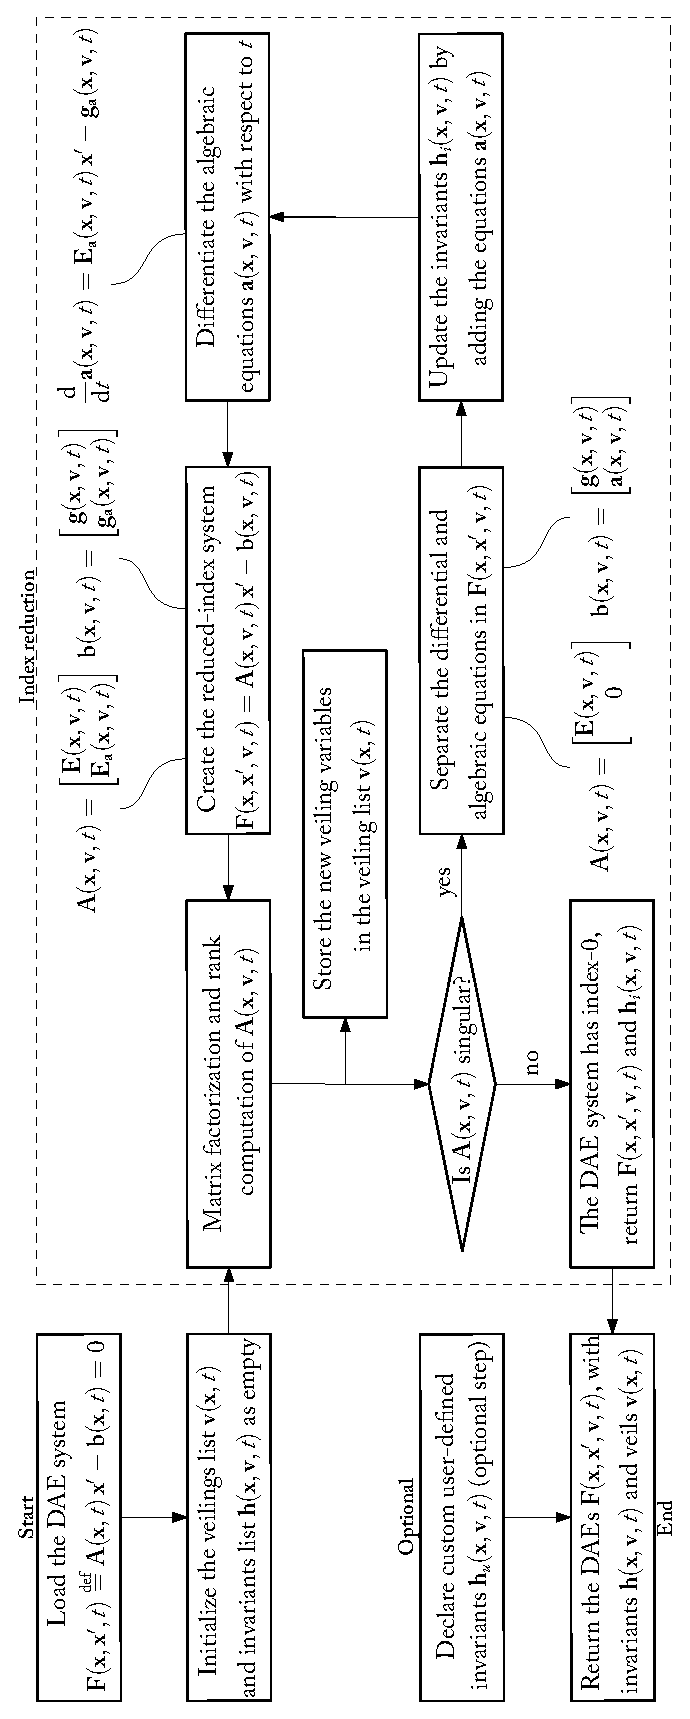
\includegraphics[angle=270, width=\textwidth]{dae_flowchart_veil}
  \caption{Flowchart of the index reduction algorithm with expression swell mitigation.}
  \label{chap4:fig:index_reduction_veil}
\end{sidewaysfigure}

% % % % % % % % % % % % % % % % % % % % % % % % % % % % % % % % % % % % % % % %

\section{The Symbolic-Numeric Solution Scheme}
\label{chap4:sec:indigo}

After this fairly long discussion on the actual implementation aspects of the index reduction algorithm, we can now present the \Indigo{} index reduction and integration toolbox~\cite{indigo}. This toolbox consists of two main components: a \Maple{} package to carry out symbolic index reduction of \ac{DAE} systems, and a \Matlab{} toolbox to perform numerical integration of the reduced-index system. \Indigo{} is designed to be used in conjunction with the \LEM{} package, to limit the expression swell, and the \LAST{} package, to conveniently factorize matrices. In the following paragraphs, we briefly discuss the usage of the \Indigo{} package.

\subsection{Index Reduction}

The index reduction algorithm implemented in the \Indigo{} \Maple{} package is the one presented in Section~\ref{chap4:sec:algorithm}. To reduce the index of a \ac{DAE} system in the \Maple{} environment we need to first create an \Indigo{} object instance.
%
\begin{verbatim}
> Indigo_obj := Object(Indigo);
> Indigo_obj:-InitLAST();
\end{verbatim}
%
Then, the system of \acp{DAE} \texttt{eqns} with coordinates \texttt{vars} is loaded.
%
\begin{verbatim}
> Indigo_obj:-LoadEquations('Generic', eqns, vars);
\end{verbatim}
%
The \texttt{Generic} symbol is used to specify the type of the system. Notice that in this example, we assume that the equations of the system are already available in the \Maple{} session. The automatic index reduction process can be performed by calling the \texttt{ReduceIndex} method, which iterates the separation and differentiation steps until an index-$0$ \ac{DAE} system is obtained.
%
\begin{verbatim}
> Indigo_obj:-ReduceIndex();
\end{verbatim}
%
Intermediate results of the process are stored internally in the \Indigo{} object and are available on demand. Once the index reduction process is completed, the user can generate the \texttt{name} \Matlab{} class file to perform numerical integration of the reduced-index system.
%
\begin{verbatim}
> Indigo_obj:-GenerateMatlabCode(name, type, data=pars);
\end{verbatim}
%
A file \texttt{name.m} is generated in the current directory. As it is explained in the next section, The string parameter \texttt{type} can be either \texttt{Implicit}, \texttt{SemiExplicit} or \texttt{Explicit} depending on the desired numerical integration scheme. The optional parameter \texttt{data} introduces default internal object data.

\subsection{Numerical Integration Scheme}

The \Indigo{} \Matlab{} toolbox is an object-oriented library that allows the user to exploit the automatically generated code of the reduced-index system. It is capable of integrating systems of \acp{ODE} and \acp{DAE} using a variety of \ac{RK} numerical integration schemes. In particular, the system of equations which is integrated is composed of the following elements.
%
\begin{itemize}
  \setlength{\itemsep}{0.0em}
  \item A differential part, which can be expressed by one of the following classes:
  %
  \begin{equation*}
      \begin{array}{ccl}
          \m{F}(\mx, \mx^\prime, \m{v}, t) = \m{0} & \hspace{0.5cm} &
          \text{\texttt{Implicit} system class,} \\[0.5mm]
          \m{A}(\mx, \m{v}, t) \, \mx^\prime = \m{b}(\mx, \m{v}, t) & \hspace{0.5cm} &
          \text{\texttt{SemiExplicit} system class,} \\[0.5mm]
          \mx^\prime = \m{f}(\mx, \m{v}, t) & \hspace{0.5cm} &
          \text{\texttt{Explicit} system class.}
      \end{array}
  \end{equation*}
  %
  \item The invariants, composed of the hidden constraints obtained from the index reduction process $\mhiv$, and optional user-defined invariants $\mhuv$, namely
  %
  \begin{equation*}
    \m{h}(\mx, \m{v}, t) = \begin{bmatrix}
        \mhiv \\[0.5mm]
        \mhuv
    \end{bmatrix} = \m{0} \, \text{.}
  \end{equation*}
  %
  \item The veils, which are the set of the expression hierarchical representation variables used in \LEM{} to limit the expression swell
  %
  \begin{equation*}
      \m{v}(\mx, t) = \begin{bmatrix}
          v_{1}(\mx, t) \\[0.5mm]
          v_{2}(v_{1}, \mx, t) \\
          \vdots \\
          v_{n}(v_{1}, \dots, v_{n-1}, \mx, t)
      \end{bmatrix} \, \text{.}
  \end{equation*}
\end{itemize}

To respect the invariants during the integration the \emph{standard projection} method is applied~\cite{hairer2000symmetric}. This method consists of projecting the solution $\mx$ of the numerically integrated reduced-index system onto the invariants manifold $\m{h}(\mx, \m{v}, t) = \m{0}$, which is equivalent to the following constrained minimization
%
\begin{equation*}
  \underset{\widetilde{\mx}}{\textrm{minimize}} \quad \dfrac{1}{2}\left(\mx - \widetilde{\mx}\right)^2
    \quad \textrm{subject to} \quad
    \m{h}(\mx, \m{v}, t) = \m{0}.
\end{equation*}

To integrate the system generated through the \Matlab{} package or a custom system \texttt{sys}, the user must first instantiate a \Indigo{} \ac{RK} solver.
%
\begin{verbatim}
>>> solver = IndigoSolver('solver_name');
>>> solver.set_system(sys);
\end{verbatim}
%
Once the solver is instantiated, it is only necessary to specify the \acp{IC} and the integration time vector.
%
\begin{verbatim}
>>> [x, t, v, h] = solver.solve(t_ini:d_t:t_end, ics);
\end{verbatim}
%
The solver returns the solution of the system in the form of multiple outputs: \texttt{x} contains the integrated solution, \texttt{x\_dot} the states' time derivative, \texttt{t} the time vector, \texttt{v} the veiling variables, and finally \texttt{h} the values of the invariants over the specified time mesh \texttt{t\_ini:d\_t:t\_end}.

\subsection{Proving the Algorithm Implementation}
\label{chap4:sec:example}

In this section, we showcase an example of a high-index \ac{DAE} system: an index-3 problem with an analytical solution, which describes the motion of a particle on a 3D torus surface~\cite{campbell1995constraint}. This example is employed to validate the numerical stability of the reduced-index system, as well as the good conditioning of both the symbolic matrix factorization and the numerical integration scheme. To ease the understanding of the results, we purposely avoid the use of the veiling variables in this example. However, the veiling variables just add an evaluation layer to the expressions, and they do not affect the numerical properties of the integrator.

\subsubsection{Expression Complexity of the Reduced-Index Systems}
\label{chap4:sec:daes_complexity}

As a first demonstration of the proposed index reduction algorithm capabilities, we first consider the given example from a purely symbolic perspective. In particular, we consider the computational cost of the expressions generated during the presented procedure, both with \ac{LU} and \ac{FFLU} factorization of the system matrix. The compactness of the expressions generated during the index reduction algorithm is a crucial aspect, as it ensures that limited computational overhead is introduced in the numerical integration of the reduced-index system, as well as in the projection of the solution on the hidden constraints. Specifically, the index reduction algorithm is applied to the \ac{DAE} system and reduced to index-0. For each reduction stage of the example considered, the computational cost is reported in Table~\ref{chap4:tab:torus}. Notably, the results show that the expression complexity is similar for both \ac{LU} and \ac{FFLU} factorization, with a slight increase in the number of multiplications and divisions for the latter.

\begin{table}[htb]
  \caption{Expression complexity encountered throughout the index reduction of the particle motion \ac{DAE} system with both the \ac{LU} and \ac{FFLU} factorization techniques. \emph{Legend}: $\cf$ = functions, $\ca$ = additions, $\cm$ = multiplications, and $\cd$ = divisions.}
  \label{chap4:tab:torus}
  \centering
  {\small\begin{tabular}{cccc}
    \multicolumn{4}{c}{\textbf{Particle Motion} (LU Factorization)~\cite{campbell1995constraint}} \\
    \toprule
    \textbf{Original \acp{DAE}} & \multicolumn{3}{c}{$\mF = 47\cf + 30\cm + 23\ca$ \quad $\mh = 0$} \\
    \midrule
    \textbf{Reduction step} & $\mE$ & $\mg$ & $\ma$ \\
    \midrule
    Index-3 \acp{DAE} & $0$ & $39\cf + 36\cm + 13\ca$ & $7\cf + 10\cm + 6\ca$ \\
    Index-2 \acp{DAE} & $0$ & $39\cf + 36\cm + 13\ca$ & $22\cf + 20\cm + 8\ca$ \\
    Index-1 \acp{DAE} & $0$ & $39\cf + 36\cm + 13\ca$ & $68\cf + 72\cm + 33\ca$ \\
    Index-0 \acp{DAE} & $388\cf + 424\cm + 180\ca$ & $79\cf + 77\cm + 26\ca$ & $0$ \\
    \midrule
    \textbf{Reduced \acp{DAE}} & \multicolumn{3}{c}{$\mF = 258\cf + 239\cm + 109\ca$ \quad $\mh = 97\cf + 102\cm + 47\ca$} \\
    \bottomrule \\[0.5em]
    %
    \multicolumn{4}{c}{\textbf{Particle Motion} (FFLU Factorization)~\cite{campbell1995constraint}} \\
    \toprule
    \textbf{Original \acp{DAE}} & \multicolumn{3}{c}{$\mF = 47\cf + 30\cm + 23\ca$ \quad $\mh = 0$} \\
    \midrule
    \textbf{Reduction step} & $\mE$ & $\mg$ & $\ma$ \\
    \midrule
    Index-3 \acp{DAE} & $0$ & $39\cf + 36\cm + 13\ca$ & $7\cf + 10\cm + 6\ca$ \\
    Index-2 \acp{DAE} & $0$ & $39\cf + 36\cm + 13\ca$ & $26\cf + 23\cm + 8\ca$ \\
    Index-1 \acp{DAE} & $0$ & $39\cf + 36\cm + 13\ca$ & $68\cf + 72\cm + 33\ca$ \\
    Index-0 \acp{DAE} & $388\cf + 424\cm + 180\ca$ & $79\cf + 77\cm + 26\ca$ & $0$ \\
    \midrule
    \textbf{Reduced \acp{DAE}} & \multicolumn{3}{c}{$\mF = 258\cf + 239\cm + 109\ca$ \quad $\mh = 97\cf + 105\cm + 47\ca$} \\
    \bottomrule
    \end{tabular}}
\end{table}

\subsubsection{Numerical Integration of the Reduced-Index System}
\label{chap4:sec:numerical_integration}

The numerical stability and consistency of the reduced-index system are demonstrated by exploiting the analytical solution of the problem in~\cite{campbell1995constraint}. Specifically, the \ac{DAE} system consists of three position variables $[x_{1}, \, x_{2}, \, x_{3}]^\top$, three velocity variables $[u_{1}, \, u_{2}, \, u_{3}]^\top$, and one constraint with Lagrange multiplier $\lambda$. The solution manifold is 4D, and the exact solution is
%
\begin{equation*}
  \mx_\text{exact} = \begin{bmatrix}
    x_{1} \\ x_{2} \\ x_{3}
  \end{bmatrix} = \begin{bmatrix}
    (\rho \cos(2\pi - t) + r) \cos(t) \\
    (\rho \cos(2\pi - t) + r) \sin(t) \\
    \rho \sin(2\pi - t)
  \end{bmatrix} \, \text{.}
\end{equation*}
%
The initial value problem is defined as follows
%
\begin{equation}
  \label{chap4:eq:torus}
  \mF = \begin{bmatrix}
    x^{\prime}_{1} - u_{1} \\
    x^{\prime}_{2} - u_{2} \\
    x^{\prime}_{3} - u_{3} \\
    u^{\prime}_{1} - u_{3}\cos(t) + x_{3}\sin(t) + u_{2} - 2 c x_{1}\lambda \\
    u^{\prime}_{2} - u_{3}\sin(t) - x_{3}\cos(t) - u_{1} - 2 c x_{2}\lambda \\
    u^{\prime}_{3} + x_{3} - 2x_{3}\lambda \\
    x_{1}^2 + x_{2}^2 + x_{3}^2 - 2r(x_{1}^2 + x_{2}^2)^{1/2} + r^2 - \rho^2
  \end{bmatrix} \, \text{,}
\end{equation}
%
with parameters $\rho = 5$ and $r = 10$, $c = 1 - {r} / {(x_{1}^2 + x_{2}^2)^{1/2}}$, states $\mx = [x_{1}, \, x_{2}, \, x_{3}, \, u_{1},$ $u_{2}, \, u_{3}, \, \lambda]^{\top}$, and \acp{IC} $\mx_{0} = [15, \, 0, \, 0, \, 0, \, 15, \, -5, \, \lambda]^{\top}$.

The numerical integration of the reduced-index system is performed through Implicit Euler, RadauIIA3, and RadauIIA5 \ac{RK} methods. To respect the invariants during the integration the \emph{standard projection} method is applied~\cite{hairer2000symmetric}. This method consists of projecting the solution $\mx$ of the numerically integrated system onto the invariants on the hidden constraints $\mh = \m{0}$, which is equivalent to the constrained minimization
%
\begin{equation*}
  \underset{\tilde{\mx}}{\textrm{minimize}} \quad \dfrac{1}{2}\left(\mx - \tilde{\mx}\right)^2
    \quad \textrm{subject to} \quad
    \mh = \m{0} \, \text{.}
\end{equation*}
%
To verify that the projection is performed correctly and does not affect the order of the \ac{RK} method, numerical integration is performed in the interval $t \in [0, \, 2\pi]$ seconds with different integration time steps $\Delta t$. The error of the numerical integration $\varepsilon = \| \mx - \mx_\text{exact} \|_{\infty}$ is reported in \figurename~\ref{chap4:fig:torus_order}. As it can be seen, the implemented projection preserves the order of the method for all the integration time steps. It is important to highlight that to obtain such results the absolute error tolerances of the integrator and the projection are both set to $\varepsilon = 10^{-10}$. The same tolerances are used in the numerical integration of the reduced-index system in the interval $t \in [0, \, 400\pi]$ seconds with step $\Delta t = 0.025$ seconds. The results are reported in \figurename~\ref{chap4:fig:torus_integration}, where Implicit Euler, RadauIIA3, and RadauIIA5 \ac{RK} methods are employed, and the projection on the hidden constraints $\mh$ is performed. The effect of the projection is highlighted on the bottom left plot.

\begin{figure}[htb]
  \centering
  \small{\includetikz{figures/chapter_4/torus_order_hidden.tex}}
  \caption{Numerical integration error $\varepsilon = \| \mx - \mx_\text{exact} \|_{\infty}$ of the \acp{DAE}~\eqref{chap4:eq:torus} over different integration time steps $\Delta t$, along with the computed order of the method (left). The projection on the hidden constraints is performed and the invariants violation $\| \mh \|_{\infty}$ is reported (right). Notice that the implemented projection preserves the order of the method for all the integration time steps. The tests are performed in $t \in [0, \, 2\pi]$ seconds, using Implicit Euler, RadauIIA3, and RadauIIA5 \ac{RK} methods.}
  \label{chap4:fig:torus_order}
\end{figure}

\begin{figure}[htbp]
  \centering
  \small{\includetikz{figures/chapter_4/torus_implicit_euler.tex}}%
  \hspace{0.25cm}%
  \small{\includetikz{figures/chapter_4/torus_radauiia3.tex}}
  \small{\includetikz{figures/chapter_4/torus_radauiia5.tex}}%
  \hspace{0.25cm}%
  \small{\includetikz{figures/chapter_4/torus_radauiia5_noproj.tex}}
  \caption{Numerically integrated solution of the \acp{DAE}~\eqref{chap4:eq:torus} in the interval $t \in [0, \, 400\pi]$ seconds, with step $\Delta t = 0.025$ seconds, using Implicit Euler (top left), RadauIIA3 (top right), and RadauIIA5 (bottom left and right) \ac{RK} methods.}
  %The first three plots show the numerical integration of the reduced-index system with projection on the hidden constraints $\mh$ produced by the index reduction algorithm. On the bottom right plot, the numerical integration of the reduced-index system is performed without projection on the manifold $\mh$ and substantial drift is observed.}
  \label{chap4:fig:torus_integration}
\end{figure}

% % % % % % % % % % % % % % % % % % % % % % % % % % % % % % % % % % % % % % % %
%%!TEX root = ../main.tex

\chapter{Application Fields and Examples}
\label{chap5:applications}

In the previous chapter, we presented a methodology for the automatic index reduction of \ac{DAE} systems. The index reduction algorithm is based on the separation of the system into differential and algebraic parts with the help of symbolic linear algebra, \ie{}, \ac{LU} or \ac{FFLU} matrix factorization. No information on the \ac{DAE} system structure is leveraged during the reduction algorithm and, for this reason, this methodology can be applied to generic \acp{DAE} linear in the state derivatives. Numerical integration goodness is showcased by assessing the order of the numerical integration scheme and the accuracy of the projection. In this chapter, we take for granted the correctness of the proposed methodology and we focus on the application and capabilities of the index reduction algorithm. Hence, the algorithm is applied to a variety of \ac{DAE} systems, which are specifically chosen to demonstrate the capabilities, the potential, as well as the wide range of applicability of the proposed methodology. The examples are divided into three main categories: \emph{multibody dynamics}, \emph{trajectory prescribed path control}, and \emph{electrical networks}. Each of these categories is characterized by a different structure of the \ac{DAE} system, which will be analyzed in detail and will help us to understand the effectiveness of the proposed methodology. The examples are mainly taken from the testsets~\cite{lioen1998test, mazzia2003test, mazzia2008test, mazzia2012test} and are the following.
%
\begin{enumerate}
  \setlength\itemsep{0.0em}
  \item Multibody dynamics field:
  \begin{enumerate}
    \setlength\itemsep{0.0em}
    \item car-axis system~\cite{lioen1998test, mazzia2008test};
    \item flexible slider-crank mechanism~\cite{lioen1998test, mazzia2008test};
    \item the multi-pendula system~\cite{nedialkov2008solvingIII};
    \item double-wishbone suspension system~\cite{lioen1998test, mazzia2008test}.
  \end{enumerate}
  \item Trajectory prescribed path control applications:
  \begin{enumerate}
    \setlength\itemsep{0.0em}
    \item initial stage space shuttle reentry problem~\cite{brenan1995numerical};
    \item final stage space shuttle reentry problem~\cite{brenan1995numerical};
    \item the robotic arm system~\cite{pryce1998solving}.
  \end{enumerate}
  \item Electrical networks field:
  \begin{enumerate}
    \setlength\itemsep{0.0em}
    \item eight-nodes transistor-amplifier~\cite{lioen1998test, mazzia2008test};
    \item electric ring modulator~\cite{lioen1998test, mazzia2008test};
    \item cascaded differential amplifier~\cite{brenan1995numerical}.
  \end{enumerate}
\end{enumerate}

A comparison between the built-in joint index reduction algorithm and numerical integration schemes offered by \Maple{} with those of \Indigo{} will demonstrate the effectiveness of the proposed methodology and software implementation. It must be pointed out that, to ensure a fair comparison, the same numerical integration method is used in both software packages, \ie{}, the \ac{RKF} 4(5) method with a relative tolerance of $10^{-6}$ and an absolute tolerance of $10^{-7}$. Only when it is not possible to integrate the system with the chosen method, the integration is performed with the RadauIIA5 method in \Indigo{} and the implicit Rosenbrock 3(4) method in \Maple{}. The computation time limit is set to \SI{100}{\second} for both index reduction and code generation. Numerical integration is not limited by time, but the results are reported only if the integration is thoroughly completed.

For the sake of completeness, we also compare \emph{some} of our results with those obtained by the \Matlab{} symbolic toolbox, which works under a \MuPAD{} \ac{CAS}. Notably, \Matlab{} is capable of performing \acp{DAE} index reduction through either the Pantelides algorithm (\texttt{reduceDAEToODE} function)~\cite{pantelides1988consistent} or the Gaussian elimination method (\texttt{reduceDAEIndex} function). The latter is claimed to be more robust and, to some extent, might be similar to the approach proposed in this work, although its working principles are not fully disclosed and its success is guaranteed only if semilinear \ac{DAE} systems are considered. However, the Pantelides algorithm is reported to be less robust and to have a higher computational cost~\cite{matlabdaes}. For the same examples, we also include the results obtained by the \Mathematica{} symbolic toolbox, which is capable of performing \acp{DAE} index reduction through the Pantelides algorithm as well. It is worth noticing that \Mathematica{} does not provide access to the reduced index \ac{DAE} system, moreover, \Matlab{} has no built-in function to compute the computational cost of each equation in the reduced-index \ac{DAE} system. This makes the comparison with the proposed methodology and software package more challenging. For this reason, we will only limit our considerations to overall performance, \ie{}, the success of both index reduction process and numerical integration processes. A summary of this comparison will be later reported in Table~\eqref{chap5:tab:numerical_integration}.

But before we proceed with the examples, it is also worth mentioning that during the index reduction process, the trigonometric identities provided by Weierstra{\ss}~\eqref{chap3:eq:weierstrass} or~\eqref{chap3:eq:zhou} can be used to slightly reformulate the \acp{DAE}expressions, as well as to obtain polynomials expressions and improve the detection of symbolic eliminations (see Section~\ref{chap3:sec:signature}). However, the use of such trigonometric identities does not typically lead to a significant improvement in the computational cost of the expressions generated during the index reduction procedure as the polynomial expressions obtained are hard to simplify as well. Furthermore, such transformations impose a change of coordinates in the original \ac{DAE} system, which may be undesirable in some applications. For this reason, no reformulation is performed in the examples presented in this chapter.

\section{Multibody Dynamics}
\label{chap5:sec:mbd}

Historically, the \ac{MBD} problems appeared in the early 60s when the first computer simulations of mechanical systems were performed. Over the years, such systems have been studied extensively, and many numerical or hybrid symbolic-numeric methods have been developed to solve them. As a consequence, the \ac{MBD} field has become one of the most important areas of research in the mechanical engineering domain having a wide range of applications. In this section, we present four examples of \ac{MBD} problems, which are solved using the proposed index reduction algorithm. But first, we provide a brief overview of the \ac{MBD} problems, their mathematical formulation, as well as the formal index reduction of the corresponding generic \ac{MB} \acp{DAE}.

The \ac{MBD} category is characterized by \ac{DAE} systems that describe the motion of a mechanism composed of interconnected rigid or flexible bodies. Within these systems, the differential equations represent motion equations, while the algebraic equations correspond to kinematic constraints, collectively constituting these \ac{MB} problems. Typically, such problems are posed as Hessenberg semi-explicit index-3 \acp{DAE} of the form
%
\begin{equation}
  \begin{cases}
    \m{p} = \m{q}^{\prime} \\
    \m{M}(\m{q}, \m{p}, t)\m{p}^{\prime} - \jac{\bm{\Phi}}{\m{q}}(\m{q}, t)^{\top}\bm{\lambda} = \m{f}(\m{q}, \m{p} ,t) \\
    \bm{\Phi}(\m{q}, t) = \m{0}
  \end{cases} \, \text{,}
  \qquad \text{with} \qquad \jac{\bm{\Phi}}{\m{q}}(\m{q}, t) = \dfrac{\partial}{\partial\m{q}}\bm{\Phi}(\m{q}, t)
  \, \text{,}
  \label{chap5:eq:mbd_fo}
\end{equation}
%
where $\m{q} \in \mathbb{R}^{n}$ and $\m{p} \in \mathbb{R}^{n}$ indicate respectively the generalized coordinates and the generalized velocities, $\m{M}(\m{q}, \m{p}, t) \in \mathbb{R}^{n\times n}$ is the mass matrix, $\bm{\Phi}(\m{q}, t) \in \mathbb{R}^{m}$ is the constraint vector, $\bm{\lambda} \in \mathbb{R}^{m}$ is the vector of Lagrange multipliers, and lastly $\m{f}(\m{q}, \m{p}, t) \in \mathbb{R}^{n}$ collects all the contributions from Coriolis and centrifugal effects, as well as external forces.

\paragraph{Index Reduction of Multibody Dynamics Equations}

To solve the problem in~\eqref{chap5:eq:mbd_fo}, one of the possible approaches is to transform the problem into a system of \acp{ODE} with invariants. Moreover, one may also isolate the Lagrange multipliers $\bm{\lambda}$ and write them explicitly in terms of the state variables so as to obtain an index-1 \acp{DAE} representation of the \ac{MBD} problem. In such cases, the index reduction can be performed by exploiting the structure of the problem, as well as the properties of the mass matrix $\m{M}(\m{q}, \m{p}, t)$ and constraint vector $\bm{\Phi}(\m{q}, t)$. To do so, we first need to differentiate the constraint $\bm{\Phi}(\m{q}, t)$, this yields to
%
\begin{equation}
  \dfrac{\de{}}{\de{} t}\bm{\Phi}(\m{q}, t) = \jac{\bm{\Phi}}{\m{q}}(\m{q}, t) + \jac{\bm{\Phi}}{t}(\m{q}, t) = \m{0}
  \, \text{,}
  \qquad \text{with} \qquad \jac{\bm{\Phi}}{t}(\m{q}, t) = \dfrac{\partial}{\partial t}\bm{\Phi}(\m{q}, t)
  \, \text{.}
  \label{chap5:eq:mbd_hidden_1}
\end{equation}
%
Notice that when constraint does not depend on time~\eqref{chap5:eq:mbd_hidden_1} expresses the intuitive idea that generalized velocity $\m{p}$ must be orthogonal to constraint's gradient. This provides also the opportunity to highlight that constraint $\bm{\Phi}(\m{q}, t)$ imposes relationships also at the velocity and acceleration level, \ie{},~\eqref{chap5:eq:mbd_hidden_1} restricts the set of feasible velocities. Finally, it must be noticed that~\eqref{chap5:eq:mbd_hidden_1} is still algebraic in the $\m{p}$ coordinates, thus in order to obtain a fully differential relationship, another differentiation is needed. This results in the following equation
%
\begin{equation}
  \dfrac{\de{}^2}{\de{}t^2}\bm{\Phi}(\m{q}, t) = \hes{\bm{\Phi}}{\m{q}t}(\m{q}, t)\m{p} + \jac{\bm{\Phi}}{\m{q}}(\m{q}, t)\m{p}^{\prime} + \dif{\bm{\Phi}}{tt}(\m{q}, t) = \m{0} \, \text{,}
  \label{chap5:eq:mbd_hidden_2}
\end{equation}
\begin{equation*}
  \text{with} \qquad
  \dif{\bm{\Phi}}{tt}(\m{q}, t) = \dfrac{\partial^2}{\partial t^2}\bm{\Phi}(\m{q}, t) \, \text{,}
  \qquad \text{and} \qquad
  \hes{\bm{\Phi}}{\m{q}t}(\m{q}, t) = \dfrac{\de{}}{\de{} t}\,\jac{\bm{\Phi}}{\m{q}}(\m{q}, t) \, \text{,}
\end{equation*}
%
which does not impose any algebraic constraint on the mechanical system states and leads to the following index-1 \ac{DAE} system
%
\begin{equation}
  \begin{cases}
    \m{q}^{\prime} = \m{p} \\
    \m{M}(\m{q}, \m{p}, t)\m{p}^{\prime} - \jac{\bm{\Phi}}{\m{q}}(\m{q}, t)^{\top}\bm{\lambda} = \m{f}(\m{q},\m{p},t) \\
    -\jac{\bm{\Phi}}{\m{q}}(\m{q}, t)\m{p}^{\prime} = \hes{\bm{\Phi}}{\m{q}t}(\m{q}, t)\m{p} + \dif{\bm{\Phi}}{tt}(\m{q}, t)
  \end{cases} \, \text{.}
  \label{chap5:eq:mbd_ode}
\end{equation}
%
System~\eqref{chap5:eq:mbd_ode} can be also written in compact matrix notation as
%
\begin{equation}
  \label{chap5:eq:mbd_ode_matrix}
  \begin{bmatrix}
    \m{I} & \m{0} & \m{0} \\
    \m{0}      & \m{M}(\m{q}, \m{p}, t) & -\jac{\bm{\Phi}}{\m{q}}(\m{q}, t)^{\top} \\
    \m{0}      & -\jac{\bm{\Phi}}{\m{q}}(\m{q}, t) & \m{0}
  \end{bmatrix}
  \begin{bmatrix}
    \m{q}^{\prime} \\
    \m{p}^{\prime} \\
    \bm{\lambda}
  \end{bmatrix}
  =
  \begin{bmatrix}
    \m{p} \\
    \m{f}(\m{q},\m{p},t) \\
    \hes{\bm{\Phi}}{\m{q}t}(\m{q}, t)\m{p} + \dif{\bm{\Phi}}{tt}(\m{q}, t)
  \end{bmatrix} \, \text{.}
\end{equation}
%
It is easy to notice that if the left-hand side matrix of~\eqref{chap5:eq:mbd_ode_matrix} is invertible, then we can write the system in explicit form. In specific, the matrix is invertible if and only if the sub-block
%
\begin{equation*}
  \begin{bmatrix}
    \m{M}(\m{q}, \m{p}, t) & -\jac{\bm{\Phi}}{\m{q}}(\m{q}, t)^{\top} \\
    -\jac{\bm{\Phi}}{\m{q}}(\m{q}, t) & \m{0}
  \end{bmatrix}
  \in\mathbb{R}^{(n+m)\times(n+m)}
\end{equation*}
%
is non-singular. To prove its non-singularity the rank additivity formula is applied as follows
%
\begin{equation*}
  \mathrm{rank}\left(
  \begin{bmatrix}
    \m{M}(\m{q}, \m{p}, t) & -\jac{\bm{\Phi}}{\m{q}}(\m{q}, t)^{\top} \\
    -\jac{\bm{\Phi}}{\m{q}}(\m{q}, t) & \m{0}
  \end{bmatrix}\right)
  = \mathrm{rank}\left(\m{M}(\m{q}, \m{p}, t)\right) + \mathrm{rank}\left( \jac{\bm{\Phi}}{\m{q}}(\m{q}, t)\m{M}(\m{q}, \m{p}, t)^{-1} \jac{\bm{\Phi}}{\m{q}}(\m{q}, t)^{\top}\right) \, \text{.}
\end{equation*}
%
Since $\m{M}(\m{q}, \m{p}, t)$ is positive definite (and thus also non-singular), then $\forall\m{q} \in \mathbb{R}^{n}, \mathrm{rank}({\m{M}(\m{q}, \m{p}, t)}) = n$. Moreover, the second term in the right-hand side of the equation above is non-negative and it is zero if and only if
%
\begin{equation}
  \mathrm{rank}\left( \jac{\bm{\Phi}}{\m{q}}(\m{q}, t) \m{M}(\m{q}, \m{p}, t)^{-1} \jac{\bm{\Phi}}{\m{q}}(\m{q}, t)^{\top}\right) = m \, \text{,}
  \label{chap5:eq:compression}
\end{equation}
%
which is not generally true. However, if we assume that the constraints are \emph{locally} linearly independent, then $\forall\m{q}\in\mathbb{R}^{n},\forall t$, the rank of the Jacobian matrix $\jac{\bm{\Phi}}{\m{q}}(\m{q}, t) = m$. Therefore, the matrix in~\eqref{chap5:eq:mbd_ode_matrix} is invertible and the overall system can be written explicitly as
%
\begin{equation*}
  \begin{bmatrix}
    \m{q}^{\prime} \\ \m{p}^{\prime} \\ \bm{\lambda}
  \end{bmatrix} = \begin{bmatrix}
    \m{I} & \m{0} & \m{0} \\
    \m{0} & \m{M}(\m{q}, \m{p}, t) & -\jac{\bm{\Phi}}{\m{q}}(\m{q}, t)^{\top} \\
    \m{0} & -\jac{\bm{\Phi}}{\m{q}}(\m{q}, t) & \m{0}
  \end{bmatrix}^{-1}
  \begin{bmatrix}
    \m{p} \\
    \m{f}(\m{q},\m{p},t) \\
    \hes{\bm{\Phi}}{\m{q}t}(\m{q}, t)\m{p} + \dif{\bm{\Phi}}{tt}(\m{q}, t)
  \end{bmatrix}
\end{equation*}
%
An explicit expression for the inverse matrix above can be obtained through tedious symbolic calculations. However, regardless of the specific solution, we want to stress a very important point: by differentiating the constraint twice we are now able to explicitly write an expression for the Lagrange multipliers (index-1 variables). If the accelerations $\m{p}^{\prime}$ are isolated from~\eqref{chap5:eq:mbd_ode_matrix} and substituted into~\eqref{chap5:eq:mbd_hidden_2}, we obtain
%
\begin{equation}
  \m{p}^{\prime} = \m{M}(\m{q}, \m{q}^{\prime}, t)^{-1} \jac{\bm{\Phi}}{\m{q}}(\m{q}, t)^{\top}\bm{\lambda} + \m{M}(\m{q}, \m{q}^{\prime}, t)^{-1}\m{f}(\m{q},\m{p},t) = \m{0} \, \text{.}
  \label{chap5:eq:gen_vel}
\end{equation}
%
Then, substituting~\eqref{chap5:eq:gen_vel} into~\eqref{chap5:eq:mbd_hidden_2} we obtain the following expression
%
\begin{equation}
  \hes{\bm{\Phi}}{\m{q}t}(\m{q}, t)\m{p} + \jac{\bm{\Phi}}{\m{q}}(\m{q}, t)\m{M}(\m{q}, \m{q}^{\prime}, t)^{-1} \jac{\bm{\Phi}}{\m{q}}(\m{q}, t)^{\top}\bm{\lambda} + \jac{\bm{\Phi}}{\m{q}}(\m{q}, t)\m{M}(\m{q}, \m{q}^{\prime}, t)^{-1} \m{f}(\m{q},\m{p},t)+\dif{\bm{\Phi}}{tt}(\m{q}, t) = 0 \, \text{.}
\end{equation}
%
Here the non-singular matrix in~\eqref{chap5:eq:compression} can be easily recognized, therefore the expression for the Lagrange multipliers is given by
%
\begin{equation*}
  \bm{\lambda} = -\left(\jac{\bm{\Phi}}{\m{q}}(\m{q}, t)\m{M}(\m{q}, \m{q}^{\prime}, t)^{-1} \jac{\bm{\Phi}}{\m{q}}(\m{q}, t)^{\top}\right)^{-1} \Big(\hes{\bm{\Phi}}{\m{q}t}(\m{q}, t)\m{p} + \jac{\bm{\Phi}}{\m{q}}(\m{q}, t)\m{M}(\m{q}, \m{q}^{\prime}, t)^{-1}\m{f}(\m{q},\m{p},t) + \dif{\bm{\Phi}}{tt}(\m{q}, t)\Big) \, \text{,}
\end{equation*}
%
which can be either substituted into the explicit form of the \ac{DAE} system~\eqref{chap5:eq:mbd_ode} or properly applied to obtain a numerically efficient representation of the \ac{MBD} problem, \ie{},
%
\begin{equation*}
  \text{a set of \acp{ODE}} \qquad
  \begin{cases}
    \m{q}^{\prime} = \m{p} \\
    \m{p}^{\prime} = \dot{\m{p}}
  \end{cases} \, \text{,} \\
\end{equation*}
%
where $\dot{\m{p}}$ is obtained by solving the linear system
%
\begin{equation*}
  \begin{bmatrix}
    \m{M}(\m{q}, \m{p}, t) & -\jac{\bm{\Phi}}{\m{q}}(\m{q}, t)^{\top} \\
    -\jac{\bm{\Phi}}{\m{q}}(\m{q}, t) & \m{0}
  \end{bmatrix}
  \begin{bmatrix}
    \dot{\m{p}} \\ \bm{\lambda}
  \end{bmatrix} = \begin{bmatrix}
    \m{f}(\m{q},\m{p},t) \\
    \hes{\bm{\Phi}}{\m{q}t}(\m{q}, t)\m{p} + \dif{\bm{\Phi}}{tt}(\m{q}, t)
  \end{bmatrix} \, \text{.}
\end{equation*}

Technically, mechanical systems subject to holonomic constraints are represented by \acp{DAE} systems of index 3, \ie{}, the differential index is one plus the number of differentiations of the constraint that are needed in order to be able to eliminate the Lagrange multipliers. Otherwise, equivalently, the number of times that we need to differentiate the constraint in order to obtain a differential equation also for each of the Lagrange multipliers.

\paragraph{Explicit Matrix Inverse}

For the sake of completeness, we provide the explicit expression for the inverse of matrix in~\eqref{chap5:eq:mbd_ode_matrix}, which is given by
%
\begin{equation*}
  \begin{bmatrix}
    \m{I} & \m{0} & \m{0} \\
    \m{0} & \m{M}(\m{q}, \m{p}, t) & -\jac{\bm{\Phi}}{\m{q}}(\m{q}, t)^{\top} \\
    \m{0} & -\jac{\bm{\Phi}}{\m{q}}(\m{q}, t) & \m{0}
  \end{bmatrix}^{-1}
  =
  \begin{bmatrix}
  \m{I} & \m{0} & \m{0} \\
  \m{0} & \m{X}_{11} & \m{X}_{12} \\
  \m{0} & \m{X}_{21} & \m{X}_{22}
  \end{bmatrix}
\end{equation*}
%
where the quantities $\m{X}_{11} \in \mathbb{R}^{n \times n}$, $\m{X}_{12} \in \mathbb{R}^{n \times m}$, $\m{X}_{21} \in \mathbb{R}^{m \times n}$, and $\m{X}_{22} \in \mathbb{R}^{m \times m}$ are defined as follows
%
\begin{equation*}
    \m{X}_{11} = \m{M}(\m{q}, \m{p}, t)^{-1} - \m{M}(\m{q}, \m{p}, t)^{-1} \jac{\bm{\Phi}}{\m{q}}(\m{q}, t)^{\top} \left(\jac{\bm{\Phi}}{\m{q}}(\m{q}, t) \m{M}(\m{q}, \m{p}, t)^{-1}\jac{\bm{\Phi}}{\m{q}}(\m{q}, t)^{\top}\right)^{-1} \jac{\bm{\Phi}}{\m{q}}(\m{q}, t)\m{M}(\m{q}, \m{p}, t)^{-1} \, \text{,}
\end{equation*}
\begin{equation*}
  \m{X}_{12} = -\m{M}(\m{q}, \m{p}, t)^{-1}\jac{\bm{\Phi}}{\m{q}}(\m{q}, t)^{\top} \left(\jac{\bm{\Phi}}{\m{q}}(\m{q}, t)\m{M}(\m{q}, \m{p}, t)^{-1} \jac{\bm{\Phi}}{\m{q}}(\m{q}, t)^{\top}\right)^{-1} \, \text{,}
\end{equation*}
\begin{equation*}
  \m{X}_{21} = -\left(\jac{\bm{\Phi}}{\m{q}}(\m{q}, t) \m{M}(\m{q}, \m{p}, t)^{-1}\jac{\bm{\Phi}}{\m{q}}(\m{q}, t)^{\top}\right)^{-1} \jac{\bm{\Phi}}{\m{q}}(\m{q}, t)\m{M}(\m{q}, \m{p}, t)^{-1} \, \text{,}
\end{equation*}
\begin{equation*}
  \m{X}_{22} = -\left(\jac{\bm{\Phi}}{\m{q}}(\m{q}, t) \m{M}(\m{q}, \m{p}, t)^{-1}\jac{\bm{\Phi}}{\m{q}}(\m{q}, t)^{\top}\right)^{-1} \, \text{.}
\end{equation*}
%
Notice that $\m{X}_{12} = \m{X}_{21}^{\top}$, as expected. Moreover, the matrix $\jac{\bm{\Phi}}{\m{q}}(\m{q}, t)\m{M}(\m{q}, \m{p}, t)^{-1} \jac{\bm{\Phi}}{\m{q}}(\m{q}, t)^{\top}$ also appears in~\eqref{chap5:eq:compression}, for which invertibility must be guaranteed.

\subsection{Car-Axis Dynamics}

After the introduction of the \ac{MBD} problems, we now present the first example, which is the car-axis dynamics problem. This example is taken from~\cite{lioen1998test, mazzia2008test} and is used to model the motion of a car as riding over an uneven road. Here, the system is modeled as two springs connected to two bars. The bottom of the left tire is the origin. The chassis is represented by a bar of mass $m$, and its position is given by $\m{q} = [x_l, y_l, x_r, y_r]^\top$, as also illustrated in Figure~\ref{chap5:fig:car_axis}. The left tire is always on a flat surface, while the right tire periodically rides over a sinusoidal road surface of height $y_b(t) = h\sin(\omega t)$. The distance between the wheels is fixed, and the car chassis must always have a fixed length, hence, the following constraints are imposed
%
\begin{equation*}
  \bm{\Phi}(\m{q}) = \begin{bmatrix}
    x_l x_b - y_l y_b \\
    (x_l - x_r)^2 + (y_l - y_r)^2 - \ell^2
  \end{bmatrix} = \m{0} \, \text{.}
\end{equation*}
%
The equations of motion for the car are derived using Lagrangian mechanics. The mass matrix $\m{M}$, and the force vector $\m{f}$ are given by
%
\begin{equation*}
  \m{M}(\m{q}) = \mathrm{diag}\left(
    (\ell_0-\ell_l)\dfrac{x_l}{\ell_l},
    (\ell_0-\ell_l)\dfrac{x_l}{\ell_l},
    (\ell_0-\ell_r)\dfrac{x_r}{\ell_r},
    (\ell_0-\ell_r)\dfrac{x_r}{\ell_r}
  \right)
  \quad \text{and} \quad
  \m{f} = \left[
    0, -\varepsilon^2\dfrac{m}{2},
    0, -\varepsilon^2\dfrac{m}{2}
  \right]^{\top}
  \, \text{,}
\end{equation*}
%
where
%
\begin{equation*}
  \ell_l = \sqrt{x_l^2 + y_l^2}
  \quad \text{and} \quad
  \ell_r = \sqrt{(x_r - x_b)^2 + (y_r - y_b)^2}
\end{equation*}
%
are respectively the length of the left and right springs, $\ell_0$ is the relaxed length of both springs, $h$ is the amplitude of the bump, and $1/\varepsilon^2$ is the Hooke's constant of the springs. The parameters of the car are chosen as $\ell = \SI{1}{\meter}$, $\ell_0 = \SI{1/2}{\meter}$, $\varepsilon = 0.01$, $m = \SI{10}{\kilo\gram}$, $h = \SI{0.1}{\meter}$, and $\omega = \SI{10}{\radian\per\second}$. While the \acp{IC} according to~\cite{lioen1998test, mazzia2008test} are $\m{q}_0 = [-1/2, 0, -1/2, 0]^\top$ and $\m{p}_0 = [0, 1/2, 1, 1/2]^\top$, with an integration time interval of $t \in \RSI{0}{3}{\second}$.

\begin{figure}
  \centering
  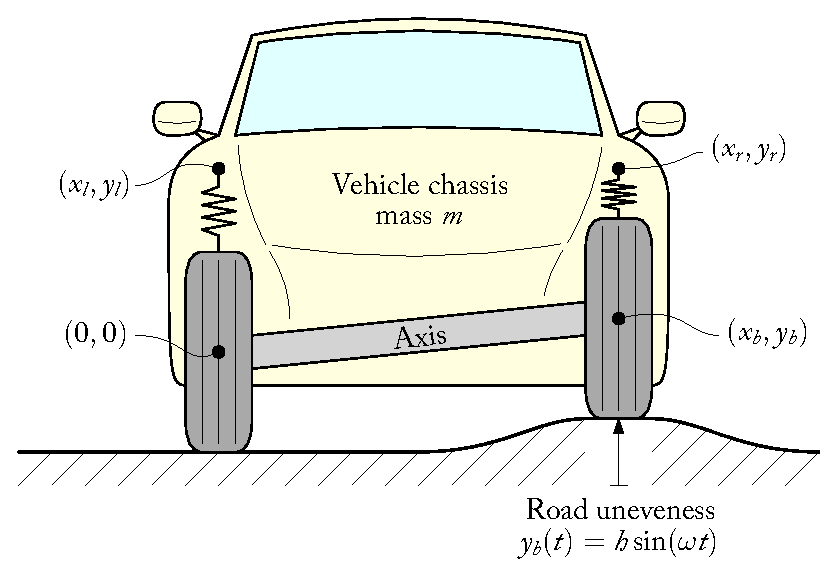
\includegraphics[width=0.7\textwidth]{figures/chapter_4/car_axis}
  \caption{Car-axis dynamics problem~\cite{lioen1998test, mazzia2008test}. The car is modeled as springs connected to two bars. The bottom of the left tire is the origin. The car chassis is represented by a bar of mass $m$. The position of the chassis is given by $\m{q} = [x_l, y_l, x_r, y_r]^\top$. The left tire is always on a flat surface, while the right tire periodically goes over a sinusoidal bump of the form $y_b(t) = h\sin(\omega t)$. The distance between the wheels must always remain fixed, and the car chassis must always have a fixed length.}
  \label{chap5:fig:car_axis}
\end{figure}

The car-axis \ac{DAE} system is solved using the proposed index reduction algorithm with both \ac{LU} and \ac{FFLU} factorization. The results are summarized in Table~\ref{chap5:tab:car_axis}. As expected, the index is reduced to 0, and the system is transformed into a set of \acp{ODE}. The complexity of the expressions encountered during the index reduction is given in terms of the number of functions $\cf$, additions $\ca$, multiplications $\cm$, and divisions $\cd$; and, as reported in the table, the index reduction is successful and little expression swell is observed only in the last reduction step. It should be noted that the \ac{FFLU} factorization produces more complex expressions than the \ac{LU} factorization and, for this reason, the former is dropped in the following simulations. The reduced system is then numerically solved using the \ac{RKF} 4(5) integrator, and the results are shown in Figure~\ref{chap5:fig:car_axis}, where the springs' lengths are plotted. Notably, during the simulation, the left spring remains nearly constant at its relaxed length, while the right spring periodically changes its length due to the bumps. It is worth mentioning that also \Mathematica{} and \Matlab{} (with both Pantelides and Gaussian elimination techniques) can correctly reduce the index of the car-axis problem and integrate the resulting system.

\begin{table}
  \caption{Expression complexity encountered throughout the index reduction of the car-axis problem~\cite{lioen1998test, mazzia2008test} \ac{DAE} system. \emph{Legend}: $\cf$ = functions, $\ca$ = additions, $\cm$ = multiplications, and $\cd$ = divisions.}
  \label{chap5:tab:car_axis}
  \centering
  {\footnotesize\begin{tabular}{cccc}
    \multicolumn{4}{c}{\textbf{Car-Axis (LU Factorization)~\cite{lioen1998test, mazzia2008test}}} \\
    \toprule
    \textbf{Original \acp{DAE}} & \multicolumn{3}{c}{$\mF = 108\cf + 131\cm + 56\ca$ \quad $\mh = 0$} \\
    \midrule
    \textbf{Reduction step} & $\mE$ & $\mg$ & $\ma$ \\
    \midrule
    Index-3 \acp{DAE} & $12\cm$ & $94\cf + 145\cm + 54\ca$ & $14\cf + 16\cm + 10\ca$ \\
    Index-2 \acp{DAE} & $12\cm$ & $94\cf + 145\cm + 54\ca$ & $26\cf + 45\cm + 15\ca$ \\
    Index-1 \acp{DAE} & $12\cm$ & $94\cf + 145\cm + 54\ca$ & $136\cf + 4\cd + 261\cm + 95\ca$ \\
    Index-0 \acp{DAE} & $1060\cf + 38\cd + 1901\cm + 717\ca$ & $431\cf + 8\cd + 842\cm + 268\ca$ & $0$ \\
    \midrule
    \textbf{Reduced \acp{DAE}} & \multicolumn{3}{c}{$\mF = 896\cf + 4\cd + 1202\cm + 546\ca$ \quad $\mh = 176\cf + 4\cd + 322\cm + 120\ca$} \\
    \bottomrule \\[0.5em]
    %
    \multicolumn{4}{c}{\textbf{Car-Axis (FFLU Factorization)~\cite{lioen1998test, mazzia2008test}}} \\
    \toprule
    \textbf{Original \acp{DAE}} & \multicolumn{3}{c}{$\mF = 108\cf + 131\cm + 56\ca$ \quad $\mh = 0$} \\
    \midrule
    \textbf{Reduction step} & $\mE$ & $\mg$ & $\ma$ \\
    \midrule
    Index-3 \acp{DAE} & $0$ & $94\cf + 8\cd + 150\cm + 54\ca$ & $14\cf + 21\cm + 10\ca$ \\
    Index-2 \acp{DAE} & $0$ & $94\cf + 8\cd + 154\cm + 54\ca$ & $26\cf + 1\cd + 44\cm + 15\ca$ \\
    Index-1 \acp{DAE} & $0$ & $94\cf + 8\cd + 155\cm + 54\ca$ & $136\cf + 6\cd + 4\cd + 261\cm + 95\ca$ \\
    Index-0 \acp{DAE} & $1066\cf + 55\cd + 1888\cm + 717\ca$ & $431\cf + 18\cd + 851\cm + 268\ca$ & $0$ \\
    \midrule
    \textbf{Reduced \acp{DAE}} & \multicolumn{3}{c}{$\mF = 1549\cf + 73\cd + 2765\cm + 1011\ca$ \quad $\mh = 176\cf + 7\cd + 326\cm + 120\ca$} \\
    \bottomrule
  \end{tabular}}
\end{table}

\begin{figure}[htb]
  \centering
  \small{\includetikz{figures/chapter_4/car_axis_length.tex}}
  \caption{Springs length of the car-axis problem~\cite{lioen1998test, mazzia2008test}. \emph{Legend}: \textcolor{mycolor1}{$\blacksquare$} left spring $L_l$, \textcolor{mycolor2}{$\blacksquare$} right spring $L_r$.}
  \label{chap5:fig:tppc_initial}
\end{figure}

\subsection{Flexible Slider-Crank Mechanism}

The slider-crank mechanism presented in Figure~\ref{chap5:fig:flexible_slider_crank} is a classic problem in mechanical engineering. The mechanism consists of a crank, a connecting rod, and a slider. The crank is driven by a motor at a constant angular velocity $\Omega$, and the slider moves back and forth in a straight line. In this case, the problem is modeled as a flexible \ac{MB} system, hence, the rod connecting the crank and the slider is modeled as a flexible beam. The flexible \ac{MBD} problem is posed as a second-order index-3 \acp{DAE} of the form
%
\begin{equation*}
  \begin{cases}
    \m{M}(\m{p}, \m{q})\begin{bmatrix}\m{p}^{\prime\prime} \\ \m{q}^{\prime\prime}\end{bmatrix} - \jac{\bm{\Phi}}{\m{p},\m{q}}(\m{p}, \m{q}, t)^{\top}\bm{\lambda} = \m{f}(\m{p}, \m{p}^{\prime}, \m{q}, \m{q}^{\prime}) \\
    \bm{\Phi}(\m{p}) = \m{0}
  \end{cases} \, \text{,}
  \qquad \text{with} \qquad \jac{\bm{\Phi}}{\m{p},\m{q}}(\m{p}, \m{q}, t) = \dfrac{\partial}{\partial(\m{p}, \m{q})}\bm{\Phi}(\m{p}, \m{q}, t)
  \, \text{,}
\end{equation*}
%
where the position or gross motion coordinates are
%
\begin{equation*}
  \m{p} = \begin{bmatrix}
    \phi_1 \\
    \phi_2 \\
    x_3
  \end{bmatrix} \quad \begin{matrix}
    \text{crank angle,} \\
    \text{connecting rod angle,} \\
    \text{sliding block displacement.}
  \end{matrix}
\end{equation*}
%
The deformation coordinates of the flexible connecting rod are
%
\begin{equation*}
  \m{q} = \begin{bmatrix}
    q_1 \\
    q_2 \\
    q_3 \\
    q_4
  \end{bmatrix} \quad \begin{matrix}
    \text{first lateral mode} \sin(\pi x/\ell_2) \, \text{,} \\
    \text{second lateral mode} \sin(2\pi x/\ell_2) \, \text{,} \\
    \text{longitudinal displacement midpoint,} \\
    \text{longitudinal displacement endpoint.}
  \end{matrix}
\end{equation*}
%
The mass matrix $\m{M}(\m{p}, \m{q})$, and the force vector $\m{f}(\m{p}, \m{q}, \m{p}^\prime, \m{q}^\prime)$ are given by
%
\begin{equation}
  \m{M}(\m{p}, \m{q}) = \begin{bmatrix}
    \m{M}_r(\m{p}) + \m{M}_e(\m{p}, \m{q}) & \m{C}(\m{p}, \m{q})^\top \\
    \m{C}(\m{p}, \m{q})                    & \m{M}_{d}
  \end{bmatrix} \, \text{,}
\end{equation}
%
with rigid motion mass matrix
%
\begin{equation*}
  \m{M}_r(\m{p}) = \begin{bmatrix}
    J_1+m_2 \ell_1^2 & \ell_1 \ell_2 m_2 \cos(\phi_1 - \phi_2)/2 & 0 \\
    \ell_1 \ell_2 m_2 \cos(\phi_1 - \phi_2)/2 & J_2 & 0 \\
    0 & 0 & m_3
  \end{bmatrix} \, \text{,}
\end{equation*}
%
coupling blocks
%
\begin{equation*}
  \m{M}_e(\m{p}, \m{q}) = \small{\begin{bmatrix}
    0 & \rho \ell_1(\cos(\phi_1 - \phi_2)\m{c}_1^\top + \sin(\phi_1 - \phi_2)\m{c}_2^\top) \m{q} & 0 \\
    \rho \ell_1(\cos(\phi_1 - \phi_2)\m{c}_1^\top + \sin(\phi_1 - \phi_2)\m{c}_2^\top) \m{q} & \m{q}^\top\m{M}_{d}\m{q} + 2\rho\m{c}_{12}^\top\m{q} & 0 \\
    0 & 0 & 0
  \end{bmatrix}}
\end{equation*}
%
and
%
\begin{equation*}
  \m{C}(\m{p}, \m{q})^\top = \begin{bmatrix}
    \rho \ell_1(\cos(\phi_1 - \phi_2)\m{c}_2^\top - \sin(\phi_1 - \phi_2)\m{c}_1^\top) \\
    \rho\m{c}_{21}^\top + \rho\m{q}^\top\m{B} \\
    \m{0}^\top
  \end{bmatrix} \, \text{,}
\end{equation*}
%
as well as elastic body space discretization mass matrix
%
\begin{equation*}
  \m{M}_{d} = \rho d h \ell_2 \begin{bmatrix}
    1/2 & 0   & 0 & 0 \\
    0   & 1/2 & 0 & 0 \\
    0   & 0   & 8 & 1 \\
    0   & 0   & 1 & 2
  \end{bmatrix} \, \text{.}
\end{equation*}
%
The force vector is given by
%
\begin{equation}
  \m{f}(\m{p}, \m{q}, \m{p}^\prime, \m{q}^\prime) = \begin{bmatrix}
    \m{f}_r(\m{p}, \m{p}^\prime) + \m{f}_e(\m{p}, \m{q}, \m{p}^\prime, \m{q}^\prime) \\
    \m{f}_{d}(\m{p}, \m{q}, \m{p}^\prime, \m{q}^\prime) - \mathrm{grad}(\m{W}_{d}(\m{q})) - \m{D}_{d} \m{q}^\prime
  \end{bmatrix} \, \text{.}
\end{equation}
%
where the rigid motion terms are collected in
%
\begin{equation*}
  \m{f}_r(\m{p}, \m{p}^\prime) = \begin{bmatrix}
    -\ell_1(\gamma(m_1 + 2m_2) \cos(\phi_1)/2 + \ell_2 m_2 \phi_2^{\prime2} \sin(\phi_1 - \phi_2)) \\
    -\ell_2 \gamma m_2 \cos(\phi_2)/2 + \ell_1 \ell_2 m_2 \phi_1^{\prime2} \sin(\phi_1 - \phi_2)/2 \\
    0
  \end{bmatrix} \, \text{.}
\end{equation*}
%
For the force term $\m{f}_e(\m{p}, \m{q}, \m{p}^\prime, \m{q}^\prime)$ the expression is
%
\begin{equation*}
  \m{f}_e(\m{p}, \m{q}, \m{p}^\prime, \m{q}^\prime) = \small{\begin{bmatrix}
    \rho \ell_1 \phi_2^{\prime2}(\cos(\phi_1 - \phi_2)\m{c}_2^\top - \sin(\phi_1 - \phi_2)\m{c}_1^\top) \m{q}-2 \rho \ell_1 \phi_2^\prime(\cos(\phi_1 - \phi_2)\m{c}_1^\top + \sin(\phi_1 - \phi_2)\m{c}_2^\top) \m{q}^\prime \\[0.5em]
    \rho \ell_1 \phi_1^{\prime2}(\sin(\phi_1 - \phi_2)\m{c}_1^\top - \cos(\phi_1 - \phi_2)\m{c}_2^\top) \m{q}-2 \rho \phi_2^\prime \m{c}_{12}^\top \m{q}^\prime-2 \phi_2^\prime {\m{q}^\prime}^\top \m{M}_{d} \m{q} \dots\\
    -\rho {\m{q}^\prime}^\top \m{B} \m{q}^\prime - \rho \gamma(\cos(\phi_2) \m{c}_1^\top \m{q} - \sin \phi_2 \m{c}_2^\top \m{q}) \\[0.5em]
    0
\end{bmatrix}} \, \text{,}
\end{equation*}
%
and for $f_{d}(\m{p}, \m{q}, \m{p}^\prime, \m{q}^\prime)$ the expression is
%
\begin{align*}
  f_{d}(\m{p}, \m{q}, \m{p}^\prime, \m{q}^\prime) &= \phi_2^{\prime2} \m{M}_{d} \m{q}+\rho(\phi_2^{\prime2} \m{c}_{12}+\ell_1 \phi_1^{\prime2}(\cos(\phi_1 - \phi_2) \m{c}_1 \dots \\
  &+ \sin(\phi_1 - \phi_2) \m{c}_2)+2 \phi_2^\prime \m{B} \m{q}^\prime)-\rho \gamma\left(\sin \phi_2 \m{c}_1+\cos(\phi_2) \m{c}_2\right) \, \text{.}
\end{align*}

The gradient of the elastic potential $\m{W}_{d}(\m{q})$ in case of linear elasticity is $\mathrm{grad}(\m{W}_{d}(\m{q})) = \m{K}_{d} \m{q}$ with the stiffness matrix
%
\begin{equation*}
  \m{K}_{d} = \dfrac{E d h}{\ell_2} \begin{bmatrix}
    \pi^4/24(h/\ell_2)^2 & 0                    & 0    & 0    \\
    0                   & \pi^4 2/3(h/\ell_2)^2 & 0    & 0    \\
    0                   & 0                     & 16/3 & -8/3 \\
    0                   & 0                     & -8/3 & 7/3
  \end{bmatrix} \, \text{.}
\end{equation*}
%
Alternatively, in the case of the nonlinear beam model, it holds $\mathrm{grad}(\m{W}_{d}(\m{q})) = K_{d}\m{q} + \m{K}_{d}(\m{q})$, where
%
\begin{equation*}
  \m{K}_{d}(\m{q}) = \dfrac{\pi^2 E d h}{2l_2^2} \begin{bmatrix}
    q_1 q_4 - \beta q_2(-4q_3 + 2q_4) \\
    4 q_2 q_4 - \beta q_1(-4q_3 + 2q_4) \\
    4 \beta q_1 q_2 \\
    q_1^2/2 + 2q_2^2 - 2 \beta q_1 q_2
  \end{bmatrix} \, \text{,}
  %
  \quad \text{with} \quad
  %
  \beta = \dfrac{80}{9\pi^2} \, \text{.}
\end{equation*}
%
The damping matrix $\m{D}_{d}$ is by default zero. The coupling matrices and vectors arising from the space discretization read
%
\begin{equation*}
  \m{B} = d h \ell_2 \begin{bmatrix}
    0             & 0         & -16/\pi^3 & 8/\pi^3-1/\pi \\
    0             & 0         & 0         & 1/(2\pi)      \\
    16/\pi^3      & 0         & 0         & 0             \\
    1/\pi-8/\pi^3 & -1/(2\pi) & 0         & 0
  \end{bmatrix} \, \text{,}
\end{equation*}
%
and
%
\begin{equation*}
  \begin{matrix}
    \m{c}_{1}  = d h \ell_2  \left[ 0,     0,         2/3, 1/6 \right]^\top \, \text{,} \\
    \m{c}_{2}  = d h \ell_2  \left[ 2/\pi, 0,         0,   0   \right]^\top \, \text{,} \\
    \m{c}_{12} = d h \ell_2^2\left[ 0,     0,         1/3, 1/6 \right]^\top \, \text{,} \\
    \m{c}_{21} = d h \ell_2^2\left[ 1/\pi, -1/(2\pi), 0,   0   \right]^\top \, \text{.}
  \end{matrix}
\end{equation*}
%
The constraints of the slider-crank mechanism are given by
%
\begin{equation*}
  \bm{\Phi}(\m{p}) = \begin{bmatrix}
    \ell_1\sin(\phi_1) + \ell_2\sin(\phi_2) + q_4\sin(\phi_2) \\
    x_3 - \ell_1\cos(\phi_1) - \ell_2\cos(\phi_2) - q_4\cos(\phi_2) \\
    \phi_1 - \Omega t \\
  \end{bmatrix} = \m{0} \, \text{.}
\end{equation*}
%
For the simulation, the following parameters are used:
%
\begin{equation*}
  \begin{matrix}
    \ell_1 = \SSI{0.15}{\meter} & \text{body 1 length,} \\
    \ell_2 = \SSI{0.30}{\meter} & \text{body 2 length,} \\
    m_1 = \SSI{0.36}{\kilo\gram} & \text{body 1 mass,} \\
    m_2 = \SSI{0.151104}{\kilo\gram} & \text{body 2 mass,} \\
    m_3 = \SSI{0.075552}{\kilo\gram} & \text{body 3 mass,} \\
    J_1 = \SSI{0.002727}{\kilo\gram\meter\squared} & \text{body 1 moment of inertia,} \\
    J_2 = \SSI{0.0045339259}{\kilo\gram\meter\squared} & \text{body 2 moment of inertia,} \\
    \rho = \SSI{7870}{\kilo\gram\per\meter\cubed} & \text{rod density,} \\
    E = \SSI{200}{\giga\newton\per\meter\squared} & \text{rod Young's modulus,} \\
    \gamma = 0 & \text{gravity constant,} \\
    \Omega = \SSI{150}{\radian\per\second} & \text{prescribed crank angular velocity.} \\
  \end{matrix}
\end{equation*}
%
The \acp{IC} according to~\cite{lioen1998test, mazzia2008test} are
%
\begin{equation*}
  \m{p}_{0} = \begin{bmatrix}
    0.000000000000000\cdot10^{+0} \\
    0.000000000000000\cdot10^{+0} \\
    4.500169330000000\cdot10^{-1}
  \end{bmatrix} \, \text{,} \qquad
  \m{p}^{\prime}_{0} = \begin{bmatrix}
     1.500000000000000\cdot10^{+2} \\
    -7.499576703969453\cdot10^{+1} \\
    -2.689386719979040\cdot10^{-6}
  \end{bmatrix} \, \text{,}
\end{equation*}
\begin{equation*}
  \m{q}_{0} = \begin{bmatrix}
    0.000000000000000\cdot10^{+0} \\
    0.000000000000000\cdot10^{+0} \\
    1.033398630000000\cdot10^{-5} \\
    1.693279690000000\cdot10^{-5}
  \end{bmatrix} \, \text{,} \qquad
  \m{q}^{\prime}_{0} = \begin{bmatrix}
     4.448961125815990\cdot10^{-1} \\
     4.634339319238670\cdot10^{-3} \\
    -1.785910760000550\cdot10^{-6} \\
    -2.689386719979040\cdot10^{-6}
  \end{bmatrix} \, \text{,}
\end{equation*}
\begin{equation*}
  \bm{\lambda}_{0} = \begin{bmatrix}
     6.552727150584648\cdot10^{-8} \\
    -3.824589509350831\cdot10^{+2} \\
     4.635908708561371\cdot10^{-9}
  \end{bmatrix} \, \text{,}
\end{equation*}
%
with an integration time interval of $t \in \RSI{0}{0.1}{\second}$.

The slider-crank mechanism \ac{DAE} system is solved with the aid of the proposed index reduction algorithm. Specifically, both the linear and nonlinear flexible beam models are considered. The results in terms of expression complexity encountered throughout the index reduction are similar for both formulations, and they are summarized in Table~\ref{chap5:tab:flexible_slider_crank}. As shown in the table, the expression complexity increases significantly during the index reduction process, which is expected due to the inherent complexity of the problem. Hierarchical representation is also employed to limit the expression swelling, and the results are summarized in Table~\ref{chap5:tab:flexible_slider_crank_veil}. The results show that the hierarchical representation reduces the expression complexity by an order of magnitude, which is beneficial for the numerical solution of the \ac{DAE} system. Nevertheless, it must be highlighted that, despite the mitigation of the expression complexity, the hierarchical representation does not prevent the expression complexity from increasing significantly during the index reduction process, which allows us to conclude that this problem is affected by inherent expression swelling. The results of the numerical simulation are shown in Figure~\ref{chap5:fig:flexible_slider_crank}, where the longitudinal displacements $q_3$ and $q_4$ of the flexible beam are illustrated. The results show that the flexible beam undergoes significant and fast deformation during the motion of the slider-crank mechanism, confirming the high stiffness of the \ac{DAE} system. In particular, the nonlinear beam model shows a more pronounced and fast deformation compared to the linear beam model, which makes the numerical solution more challenging. Indeed, the numerical solution of the slider-crank mechanism with the nonlinear beam model exhibits an overflow error after $t = \SI{0.05}{\second}$, which is likely due to either the high stiffness of the \ac{DAE} system or strongly undamped oscillations. The linear beam model, on the other hand, does not exhibit such issues and is successfully solved. It should be noticed from Figure~\ref{chap5:fig:flexible_slider_crank_pivots} that the ac{LU} pivots having minimum values are neither crossing nor getting close to zero, which is a good indicator of the numerical stability of the \ac{LU} factorization and thereby of the efficacy of the symbolic pivoting strategy.

\begin{figure}[htb]
  \centering
  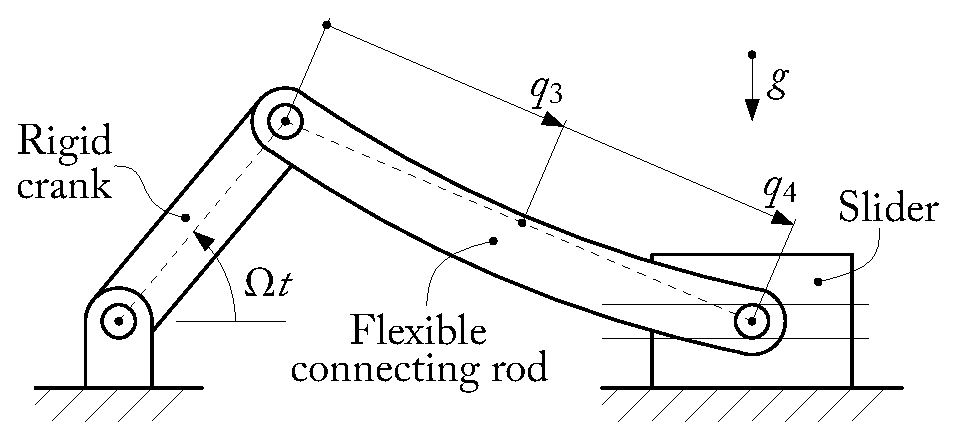
\includegraphics[width=0.475\linewidth]{flexible_slider_crank}
  \caption{Representation of the flexible slider-crank mechanism~\cite{lioen1998test, mazzia2008test}.}
  \label{chap5:fig:flexible_slider_crank}
\end{figure}

\begin{table}
  \caption{Expression complexity encountered throughout the index reduction of the flexible slider-crank mechanism problem~\cite{lioen1998test, mazzia2008test} \ac{DAE} system. \emph{Legend}: $\cf$ = functions, $\ca$ = additions, $\cm$ = multiplications, and $\cd$ = divisions.}
  \label{chap5:tab:flexible_slider_crank}
  \centering
  \resizebox{\textwidth}{!}{%
  {\footnotesize\begin{tabular}{cccc}
    \multicolumn{4}{c}{\textbf{Flexible Slider-Crank Mechanism~\cite{lioen1998test, mazzia2008test}}} \\
    \toprule
    \textbf{Original \acp{DAE}} & \multicolumn{3}{c}{$\mF = 281\cf + 10\cd + 607\cm + 144\ca$ \quad $\mh = 0$} \\
    \midrule
    \textbf{Reduction step} & $\mE$ & $\mg$ & $\ma$ \\
    \midrule
    Index-3 \acp{DAE} & $64\cf + 9\cd + 1158\cm + 167\ca$ & $395\cf + 15\cd + 5552\cm + 871\ca$ & $12\cf + 5\cm + 6\ca$ \\
    Index-2 \acp{DAE} & $64\cf + 9\cd + 1158\cm + 167\ca$ & $395\cf + 15\cd + 5552\cm + 871\ca$ & $22\cf + 10\cm + 8\ca$ \\
    Index-1 \acp{DAE} & $20\cf + 5\cd + 110\cm + 19\ca$ & $277\cf + 13\cd + 1907\cm + 326\ca$ & $\star (0.4\cf + 2.4\cm + 0.1\ca)\cdot10^{6} + 15\cd$ \\
    Index-0 \acp{DAE} & $\star (0.8\cf + 4.8\cm + 0.3\ca)\cdot10^{5} + 77\cd$ & $\star (5.8\cf + 35.7\cm + 2.2\ca)\cdot10^{6} + 1259\cd$ & $0$ \\
    \midrule
    \textbf{Reduced \acp{DAE}} & \multicolumn{3}{c}{$\star \mF = (5.8\cf + 36.2\cm + 2.2\ca)\cdot10^{6} + 1336\cd$ \quad $\star \mh = (0.5\cf + 2.4\cm + 0.1\ca)\cdot10^{6} + 15\cd$} \\
    \bottomrule
  \end{tabular}}
  }
\end{table}

\begin{table}
  \caption{Expression complexity encountered throughout the index reduction with the aid of hierarchical representation of the flexible slider-crank mechanism problem~\cite{lioen1998test, mazzia2008test} \ac{DAE} system. \emph{Legend}: $\cf$ = functions, $\cv$ = veiling variables, $\ca$ = additions, $\cm$ = multiplications, and $\cd$ = divisions.}
  \label{chap5:tab:flexible_slider_crank_veil}
  \centering
  \resizebox{\textwidth}{!}{%
  {\footnotesize\begin{tabular}{cccc}
    \multicolumn{4}{c}{\textbf{Flexible Slider-Crank Mechanism~\cite{lioen1998test, mazzia2008test}}} \\
    \toprule
    \textbf{Original \acp{DAE}} & \multicolumn{3}{c}{$\mF = 281\cf + 10\cd + 607\cm + 144\ca$ \quad $\mh = 0$} \\
    \midrule
    \textbf{Reduction step} & $\mE$ & $\mg$ & $\ma$ \\
    \midrule
    Index-3 \acp{DAE} & $28\cf + 1\cv + 7\cd + 160\cm + 28\ca$ & $91\cf + 2\cv + 8\cd + 291\cm + 44\ca$ & $12\cf + 5\cm + 6\ca$ \\
    Index-2 \acp{DAE} & $18\cf + 1\cv + 6\cd + 88\cm + 15\ca$ & $101\cf + 5\cv + 10\cd + 360\cm + 58\ca$ & $22\cf + 10\cm + 8\ca$ \\
    Index-1 \acp{DAE} & $10\cf + 1\cv + 4\cd + 39\cm + 6\ca$ & $93\cf + 4\cv + 9\cd + 294\cm + 48\ca$ & $10\cf + 2\cv + 9\cd + 82\cm + 14\ca$ \\
    Index-0 \acp{DAE} & $(0.2\cf  + 1.1\cm + 0.1\ca)\cdot10^{6} + 1171\cv + 1158\cd$ & $(0.7\cf + 3.6\cm + 0.4\ca)\cdot10^{5} + 137\cv + 1172\cd$ & $0$ \\
    \midrule
    \textbf{Reduced \acp{DAE}} & \multicolumn{3}{c}{$\mF = (0.3\cf + 1.5\cm + 0.1\ca)\cdot10^{6} + 1308\cv + 2330\cd$ \quad $\mh = 44\cf + 6\cv + 2\cd + 97\cm + 28\ca$} \\
    \bottomrule \\[0.5em]
  \end{tabular}
  }}
  {\footnotesize\begin{tabular}{cc}
    \multicolumn{2}{c}{Hierarchical representation details (9 veils)} \\
    \toprule
    \textbf{Original \acp{DAE}} & $\mv = 0$ \\
    \midrule
    \textbf{Reduction step} & $\mv$ \\
    \midrule
    Index-3 \acp{DAE} & $309\cf + 1\cv + 7\cd + 2946\cm + 485\ca$ \\
    Index-2 \acp{DAE} & $309\cf + 1\cv + 7\cd + 2946\cm + 485\ca$ \\
    Index-1 \acp{DAE} & $422\cf + 7\cv + 14\cd + 3249\cm + 541\ca$ \\
    Index-0 \acp{DAE} & $492919\cf + 63922\cv + 138\cd + 2441245\cm + 155539\ca$ \\
    \midrule
    \textbf{Reduced \acp{DAE}} & $\mv = 492919\cf + 63922\cv + 138\cd + 2441245\cm + 155539\ca$ \\
    \bottomrule
  \end{tabular}}
\end{table}

\begin{figure}[htb]
  \centering
  \small{\includetikz{figures/chapter_4/flexible_slider_crank.tex}}
  \caption{Longitudinal displacement endpoint of the in the flexible slider-crank problem~\cite{lioen1998test, mazzia2008test}. \emph{Color legend}: \textcolor{mycolor2}{$\blacksquare$} longitudinal displacement $q_3$ at the rod midpoint, and \textcolor{mycolor1}{$\blacksquare$} longitudinal displacement $q_4$ at the rod endpoint. \emph{Line legend}: \textbf{---} linear beam model, and \textbf{--~--} nonlinear beam model.}
  \label{chap5:fig:flexible_slider_crank}
\end{figure}

\begin{figure}[htb]
  \centering
  \small{\includetikz{figures/chapter_4/flexible_slider_crank_pivots.tex}}
  \caption{Representation of the two pivots of the flexible slider-crank mechanism~\cite{lioen1998test, mazzia2008test} having minimum values. \emph{Color legend}: \textcolor{mycolor1}{$\blacksquare$} pivot 1, and \textcolor{mycolor2}{$\blacksquare$} pivot 2. \emph{Line legend}: \textbf{---} linear beam model, and \textbf{--~--} nonlinear beam model.}
  \label{chap5:fig:flexible_slider_crank_pivots}
\end{figure}

\subsection{The Multi-Pendula System}

The multi-pendula system consists of a chain of $p$ coupled pendula. The first pendulum is a standard simple pendulum, while the remaining pendula are coupled to the previous one. Specifically, the tension in pendulum $i - 1$, which is represented by the Lagrange multiplier $\lambda_{i-1}$, has a small effect on the length of
pendulum $p$, for $i = 2, \dots, p$. The first-order equations of motion for the multi-pendula system are the following~\cite{nedialkov2008solvingIII}
%
\begin{equation}
  \begin{cases}
    u_1^{\prime} = x_1 \\
    v_1^{\prime} = y_1 \\
    x_1^{\prime} = -\lambda_1 x_1 \\
    y_1^{\prime} = -\lambda_1 y_1 - g \\
    x_1^2 + y_1^2 = \ell^2 \\
  \end{cases}
  \quad \text{and} \qquad
  \begin{cases}
    u_i^{\prime} = x_i \\
    v_i^{\prime} = y_i \\
    x_i^{\prime} = -\lambda_p x_i \\
    y_i^{\prime} = -\lambda_p y_i - g \\
    x_i^2 + y_i^2 = (\ell + c\lambda_{i-1})^2
  \end{cases}
  \quad \text{for} \quad i = 2, \dots, p \, \text{.}
  \label{chap5:eq:multi_pendula}
\end{equation}
%
where $x_i, y_i$ and $u_i, v_i$ are the generalized coordinates and velocities of $i$-th pendulum mass. The parameters of the multi-pendula system are chosen as $\ell = \SI{1}{\meter}$, $g = \SI{9.81}{\meter\per\second\squared}$, and $c = 0.1$. The system~\eqref{chap5:eq:multi_pendula} leads to a class of \acp{DAE} of arbitrary size $5p$ and index $2p+1$~\cite{nedialkov2008solvingIII}. \acp{IC} are chosen randomly, and the time interval is $t \in \RSI{0}{60}{\second}$.

Here, we consider up to $p = 4$ pendula, leading to a \ac{DAE} system of $20$ variables and index $9$. The computational complexities encountered during the index reduction process are summarized in Table~\ref{chap5:tab:pendula_2}, for the 2-pendula problem, Table~\ref{chap5:tab:pendula_3}, for the 3-pendula problem, Table~\ref{chap5:tab:pendula_4}, for the 4-pendula problem, and lastly, Table~\ref{chap5:tab:pendula_5}, for the 5-pendula problem. The multi-pendula systems with $p \leq 3$ exhibit low computational complexity growth during the index reduction process. However, for $p \geq 4$, there is a substantial expression swell, which makes the index reduction process time-consuming and computationally demanding, yet still feasible. The introduction of veiling variables is avoided on purpose to assess the impact of strong expression swelling on the stability of the numerical solution.
It is worth noting that with $p = 4$ the maximum computational complexity that \Maple{} can handle within a reasonable time is reached. For this reason, performing the last reduction steps for $p > 4$ requires a significant amount of time and computational resources. Furthermore, we believe that reducing the index of the \ac{DAE} system for $p > 5$ is not feasible within an acceptable time frame, even with the aid of hierarchical representation. The numerical integration results of the 5-pendula system are depicted in Figure~\ref{chap5:fig:npendula_length}, where the pendula lengths are illustrated in the time interval $t \in \RSI{0}{60}{\second}$. It must be pointed out that the numerical solution of the 5-pendula system is computed from its index-2 \ac{DAE} form, as its index-0 form demands a significant amount of computational resources and time to be solved.

\begin{table}
  \caption{Expression complexity encountered throughout the index reduction of the 2-pendula problem~\cite{nedialkov2008solvingIII} \ac{DAE} system. \emph{Legend}: $\cf$ = functions, $\ca$ = additions, $\cm$ = multiplications, and $\cd$ = divisions.}
  \label{chap5:tab:pendula_2}
  \centering
  {\footnotesize\begin{tabular}{cccc}
    \multicolumn{4}{c}{\textbf{2-Pendula~\cite{pryce1998solving}}} \\
    \toprule
    \textbf{Original \acp{DAE}} & \multicolumn{3}{c}{$\mF = 33\cf + 15\cm + 15\ca$ \quad $\mh = 0$} \\
    \midrule
    \textbf{Reduction step} & $\mE$ & $\mg$ & $\ma$ \\
    \midrule
    Index-5 \acp{DAE} & $0$                  & $12\cf + 8\cm + 2\ca$ & $6\cf + 12\cm + 6\ca$ \\
    Index-4 \acp{DAE} & $1\cf + 5\cm + 1\ca$ & $16\cf + 12\cm + 3\ca$ & $4\cf + 4\cm + 1\ca$ \\
    Index-3 \acp{DAE} & $1\cf + 5\cm + 1\ca$ & $16\cf + 12\cm + 3\ca$ & $7\cf + 12\cm + 4\ca$ \\
    Index-2 \acp{DAE} & $1\cf + 5\cm + 1\ca$ & $16\cf + 12\cm + 3\ca$ & $18\cf + 2\cd + 30\cm + 9\ca$ \\
    Index-1 \acp{DAE} & $1\cf + 5\cm + 1\ca$ & $16\cf + 12\cm + 3\ca$ & $118\cf + 2\cd + 283\cm + 72\ca$ \\
    Index-0 \acp{DAE} & $555\cf + 21\cd + 1213\cm + 287\ca$ & $16\cf + 12\cm + 3\ca$ & $0$ \\
    \midrule
    \textbf{Reduced \acp{DAE}} & \multicolumn{3}{c}{
    $\mF = 482\cf + 2\cd + 807\cm + 229\ca$ \quad $\mh = 153\cf + 4\cd + 341\cm + 92\ca$} \\
    \bottomrule
  \end{tabular}}
\end{table}

\begin{table}
  \caption{Expression complexity encountered throughout the index reduction of the 3-pendula problem~\cite{nedialkov2008solvingIII} \ac{DAE} system. \emph{Legend}: $\cf$ = functions, $\ca$ = additions, $\cm$ = multiplications, and $\cd$ = divisions.}
  \label{chap5:tab:pendula_3}
  \centering
  {\footnotesize\begin{tabular}{cccc}
    \multicolumn{4}{c}{\textbf{3-Pendula~\cite{nedialkov2008solvingIII}}} \\
    \toprule
    \textbf{Original \acp{DAE}} & \multicolumn{3}{c}{$\mF = 50\cf + 23\cm + 23\ca$ \quad $\mh = 0$} \\
    \midrule
    \textbf{Reduction step} & $\mE$ & $\mg$ & $\ma$ \\
    \midrule
    Index-7 \acp{DAE} & $0$                   & $18\cf + 12\cm + 3\ca$ & $10\cf + 21\cm + 10\ca$ \\
    Index-6 \acp{DAE} & $2\cf + 10\cm + 2\ca$ & $26\cf + 20\cm + 5\ca$ & $4\cf + 4\cm + 1\ca$ \\
    Index-5 \acp{DAE} & $2\cf + 10\cm + 2\ca$ & $26\cf + 20\cm + 5\ca$ & $7\cf + 12\cm + 4\ca$ \\
    Index-4 \acp{DAE} & $2\cf + 10\cm + 2\ca$ & $26\cf + 20\cm + 5\ca$ & $18\cf + 2\cd + 30\cm + 9\ca$ \\
    Index-3 \acp{DAE} & $2\cf + 10\cm + 2\ca$ & $26\cf + 20\cm + 5\ca$ & $118\cf + 2\cd + 283\cm + 72\ca$ \\
    Index-2 \acp{DAE} & $2\cf + 10\cm + 2\ca$ & $26\cf + 20\cm + 5\ca$ & $992\cf + 3\cd + 2077\cm + 479\ca$ \\
    Index-1 \acp{DAE} & $2\cf + 10\cm + 2\ca$ & $26\cf + 20\cm + 5\ca$ & $6824\cf + 3\cd + 17665\cm + 4030\ca$ \\
    Index-0 \acp{DAE} & $54152\cf + 51\cd + 136388\cm + 28945\ca$ & $26\cf + 20\cm + 5\ca$ & $0$ \\
    \midrule
    \textbf{Reduced \acp{DAE}} & \multicolumn{3}{c}{
    $\mF = 28319\cf + 3\cd + 64295\cm + 15806\ca$ \quad $\mh = 7973\cf + 10\cd + 20092\cm + 4605\ca$} \\
    \bottomrule
  \end{tabular}}
\end{table}

\begin{table}
  \caption{Expression complexity encountered throughout the index reduction of the 4-pendula problem~\cite{nedialkov2008solvingIII} \ac{DAE} system. \emph{Legend}: $\cf$ = functions, $\ca$ = additions, $\cm$ = multiplications, and $\cd$ = divisions.}
  \label{chap5:tab:pendula_4}
  \centering
  {\footnotesize\begin{tabular}{cccc}
    \multicolumn{4}{c}{\textbf{4-Pendula~\cite{nedialkov2008solvingIII}}} \\
    \toprule
    \textbf{Original \acp{DAE}} & \multicolumn{3}{c}{$\mF = 67\cf + 31\cm + 31\ca$ \quad $\mh = 0$} \\
    \midrule
    \textbf{Reduction step} & $\mE$ & $\mg$ & $\ma$ \\
    \midrule
    Index-9 \acp{DAE} & $0$                   & $24\cf + 16\cm + 4\ca$ & $14\cf + 30\cm + 14\ca$ \\
    Index-8 \acp{DAE} & $3\cf + 15\cm + 3\ca$ & $36\cf + 28\cm + 7\ca$ & $4\cf + 4\cm + 1\ca$ \\
    Index-7 \acp{DAE} & $3\cf + 15\cm + 3\ca$ & $36\cf + 28\cm + 7\ca$ & $7\cf + 12\cm + 4\ca$ \\
    Index-6 \acp{DAE} & $3\cf + 15\cm + 3\ca$ & $36\cf + 28\cm + 7\ca$ & $18\cf + 2\cd + 30\cm + 9\ca$ \\
    Index-5 \acp{DAE} & $3\cf + 15\cm + 3\ca$ & $36\cf + 28\cm + 7\ca$ & $118\cf + 2\cd + 283\cm + 72\ca$ \\
    Index-4 \acp{DAE} & $3\cf + 15\cm + 3\ca$ & $36\cf + 28\cm + 7\ca$ & $992\cf + 3\cd + 2077\cm + 479\ca$ \\
    Index-3 \acp{DAE} & $3\cf + 15\cm + 3\ca$ & $36\cf + 28\cm + 7\ca$ & $6824\cf + 3\cd + 17665\cm + 4030\ca$ \\
    Index-2 \acp{DAE} & $3\cf + 15\cm + 3\ca$ & $36\cf + 28\cm + 7\ca$ & $(4.8\cf + 4\cd + 11.9\cm + 2.7\ca)\cdot10^{5}$ \\
    Index-1 \acp{DAE} & $3\cf + 15\cm + 3\ca$ & $36\cf + 28\cm + 7\ca$ & $\star (3.0\cf + 14.9\cm + 0.4\ca)\cdot10^{6} + 4\cd$ \\
    Index-0 \acp{DAE} & $\star (3.0\cf + 14.7\cm + 0.4\ca)\cdot10^{7} + 92\cd$ & $30\cf + 28\cm + 7\ca$ & $0$ \\
    \midrule
    \textbf{Reduced \acp{DAE}} & \multicolumn{3}{c}{
    $\star \mF = (3.0\cf + 14.7\cm + 0.4\ca)\cdot10^{7} + 92\cd$ \quad $\star \mh = (3.1\cf + 15.1\cm + 0.5\ca)\cdot10^{6} + 18\cd$} \\
    \bottomrule
  \end{tabular}}
\end{table}

\begin{table}
  \caption{Expression complexity encountered throughout the index reduction of the 5-pendula problem~\cite{nedialkov2008solvingIII} \ac{DAE} system. \emph{Legend}: $\cf$ = functions, $\ca$ = additions, $\cm$ = multiplications, and $\cd$ = divisions.}
  \label{chap5:tab:pendula_5}
  \centering
  {\footnotesize\begin{tabular}{cccc}
    \multicolumn{4}{c}{\textbf{5-Pendula~\cite{nedialkov2008solvingIII}}} \\
    \toprule
    \textbf{Original \acp{DAE}} & \multicolumn{3}{c}{$\mF = 84\cf + 39\cm + 39\ca$ \quad $\mh = 0$} \\
    \midrule
    \textbf{Reduction step} & $\mE$ & $\mg$ & $\ma$ \\
    \midrule
    Index-11 \acp{DAE} & $0$                   & $30\cf + 20\cm + 5\ca$ & $18\cf + 39\cm + 18\ca$ \\
    Index-10 \acp{DAE} & $4\cf + 20\cm + 4\ca$ & $46\cf + 36\cm + 9\ca$ & $4\cf + 4\cm + 1\ca$ \\
    Index-9 \acp{DAE}  & $4\cf + 20\cm + 4\ca$ & $46\cf + 36\cm + 9\ca$ & $7\cf + 12\cm + 4\ca$ \\
    Index-8 \acp{DAE}  & $4\cf + 20\cm + 4\ca$ & $46\cf + 36\cm + 9\ca$ & $18\cf + 2\cd + 30\cm + 9\ca$ \\
    Index-7 \acp{DAE}  & $4\cf + 20\cm + 4\ca$ & $46\cf + 36\cm + 9\ca$ & $118\cf + 2\cd + 283\cm + 72\ca$ \\
    Index-6 \acp{DAE}  & $4\cf + 20\cm + 4\ca$ & $46\cf + 36\cm + 9\ca$ & $992\cf + 3\cd + 2077\cm + 479\ca$ \\
    Index-5 \acp{DAE}  & $4\cf + 20\cm + 4\ca$ & $46\cf + 36\cm + 9\ca$ & $6824\cf + 3\cd + 17665\cm + 4030\ca$ \\
    Index-4 \acp{DAE}  & $4\cf + 20\cm + 4\ca$ & $46\cf + 36\cm + 9\ca$ & $(4.8\cf + 4\cd + 11.9\cm + 2.7\ca)\cdot10^{5}$ \\
    Index-3 \acp{DAE}  & $4\cf + 20\cm + 4\ca$ & $46\cf + 36\cm + 9\ca$ & $\star (3.0\cf + 14.9\cm + 0.4\ca)\cdot10^{6} + 4\cd$ \\
    Index-2 \acp{DAE}  & $4\cf + 20\cm + 4\ca$ & $46\cf + 36\cm + 9\ca$ & $\star (5.1\cf + 4.0\cm + 1.3\ca)\cdot10^{7} + 5\cd$ \\
    Index-1 \acp{DAE}  & $4\cf + 20\cm + 4\ca$ & $46\cf + 36\cm + 9\ca$ & $\star (9.1\cf + 11.3\cm + 5.9\ca)\cdot10^{7} + 5\cd$ \\
    Index-0 \acp{DAE}  & $\star (8.8\cf + 7.2\cm + 1.0\ca)\cdot10^{8} + 5\cd$ & $46\cf + 36\cm + 9\ca$ & $0$ \\
    \midrule
    \textbf{Reduced \acp{DAE}} & \multicolumn{3}{c}{
    $\star \mF = \star (8.8\cf + 7.2\cm + 1.0\ca)\cdot10^{8} + 5\cd$ \quad $\star \mh = (9.2\cf + 6.5\cm + 1.0\ca)\cdot10^{7} + 18\cd$} \\
    \bottomrule
  \end{tabular}}
\end{table}

\begin{figure}[htb]
  \centering
  \small{\includetikz{figures/chapter_4/npendula_length.tex}}
  \caption{Pendula lengths of the multi-pendula problem~\cite{nedialkov2008solvingIII} (up to 5 pendula). \emph{Legend}: \textcolor{mycolor1}{$\blacksquare$} 1\textsuperscript{st} pendulum length $\ell_1 = \ell$, \textcolor{mycolor2}{$\blacksquare$} 2\textsuperscript{nd} pendulum length $\ell_2 = \ell + c\lambda_1$, \textcolor{mycolor3}{$\blacksquare$} 3\textsuperscript{rd} pendulum length $\ell_3 = \ell + c\lambda_2$, \textcolor{mycolor4}{$\blacksquare$} 4\textsuperscript{th} pendulum length $\ell_4 = \ell + c\lambda_3$, and \textcolor{mycolor5}{$\blacksquare$} 5\textsuperscript{th} pendulum length $\ell_5 = \ell + c\lambda_4$.}
  \label{chap5:fig:npendula_length}
\end{figure}

\subsection{Double-Wishbone Suspension System}

As a final example for this application field, we consider a double-wishbone suspension system.

\subsubsection{Suspension System Modeling}

Double A-arm or double wishbone suspensions are independent suspension systems widely used in the automotive industry, especially in high-performance vehicles, due to their superior handling characteristics. The studied double A-arm suspension system, shown in Figure~\ref{chap5:fig:suspension_render} is characterized by two A-shaped arms, one upper and one lower, connected to the chassis at one end and to the wheel carrier at the other end forming, together with the tie rod, the principal kinematic chain of the suspension system. A second kinematic chain is formed by the push rod and the rocker, which transfer the vertical load from the wheel carrier to the shock absorber.

\begin{figure}[htb]
  \begin{minipage}[c]{0.485\linewidth}
    \centering
    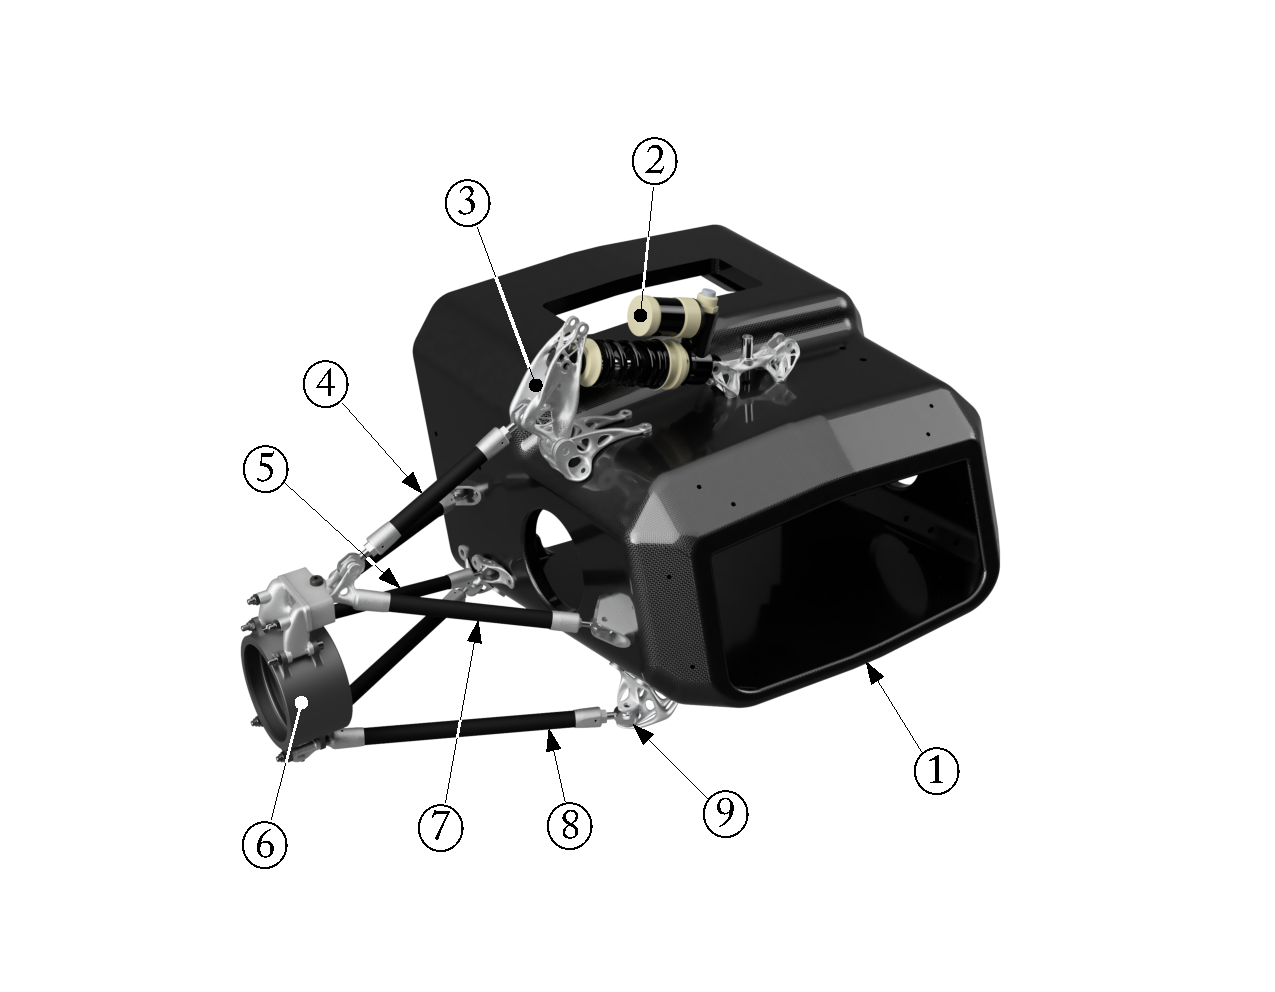
\includegraphics[width=1.0\textwidth, trim={3.0cm 1.5cm 4.0cm 1.7cm}, clip]{figures/chapter_4/suspension_render.eps}
  \end{minipage}
  %\hfill
  \begin{minipage}[c]{0.45\linewidth}
    \centering
    \small{\begin{tabular}{ccc}
      \toprule
      \multirow{2}{*}{\textbf{\#}} & \multirow{2}{*}{\textbf{Component}} & \textbf{\TrussMe{}} \\
      & & \textbf{type} \\
      \midrule
      \circled{\small{1}} & Carbon fiber cell & Rigid support    \\[1.25mm]
      \circled{\small{2}} & Shock absorber    & Constrained node \\[1.25mm]
      \circled{\small{3}} & Rocker            & Generic element  \\[1.25mm]
      \circled{\small{4}} & Push rod          & Rod element      \\[1.25mm]
      \circled{\small{5}} & Tie rod           & Rod element      \\[1.25mm]
      \circled{\small{6}} & Wheel carrier     & Generic element  \\[1.25mm]
      \circled{\small{7}} & Upper wishbone    & Beam elements    \\[1.25mm]
      \circled{\small{8}} & Lower wishbone    & Beam elements    \\[1.25mm]
      \circled{\small{9}} & Rod end           & Compliant node    \\
      \bottomrule
    \end{tabular}}
  \end{minipage}
  \caption{Rendering and description of the \TrussMe{} elements \citep{trussme} used to model the rear left double wishbone suspension of the Formula SAE \textit{E-Agle Trento Racing Team} vehicle~\citep{eagle}.}
  \label{chap5:fig:suspension_render}
\end{figure}

In this example, the double A-arm suspension compliance is modeled using macro elements, which are modeled through the \TrussMe{} package~\cite{trussme}, which is a \Maple{} package for the symbolic modeling of compliant structures. Details on the modeling of the compliant elements are reported in Appendix~\ref{app4:trussme}. With the approach there presented, two suspension compliance models are generated one does not include the bushings compliance, while the other does. The linear systems have different sizes depending on the number of \acp{DOF} considered. In the case of the suspension without bushings, the system is composed of 78 \acp{DOF}, and has the following form
%
\begin{equation}
  \begin{bmatrix}
    \m{K}_{ff ,\, 42 \times 42}(\mathbb{R}) & \m{K}_{fs ,\, 42 \times 36}(\mathbb{R}) \\
    \m{K}_{sf ,\, 36 \times 42}(\mathbb{R}) & \m{K}_{ss ,\, 36 \times 36}(\mathbb{R})
  \end{bmatrix} \begin{bmatrix}
    \m{d}_{f ,\, 42 \times 1}(\mathbb{R}) \\ \m{d}_{s ,\, 36 \times 1}(\mathbb{R})
  \end{bmatrix} = \begin{bmatrix}
    \m{f}_{f ,\, 42 \times 1}(\mathbb{R}) \\ \m{f}_{s ,\, 36 \times 1}(\mathbb{R})
  \end{bmatrix}
  \, \text{.}
\end{equation}
%
On the other hand, the suspension model with the bushings influence is composed of 138 \acp{DOF}
%
\begin{equation}
  \begin{bmatrix}
    \m{K}_{ff ,\, 72 \times 72}(\mathbb{R}) & \m{K}_{fs ,\, 72 \times 66}(\mathbb{R}) \\
    \m{K}_{sf ,\, 66 \times 72}(\mathbb{R}) & \m{K}_{ss ,\, 66 \times 66}(\mathbb{R})
  \end{bmatrix} \begin{bmatrix}
    \m{d}_{f ,\, 72 \times 1}(\mathbb{R}) \\ \m{d}_{s ,\, 66 \times 1}(\mathbb{R})
  \end{bmatrix} = \begin{bmatrix}
    \m{f}_{f ,\, 72 \times 1}(\mathbb{R}) \\ \m{f}_{s ,\, 66 \times 1}(\mathbb{R})
  \end{bmatrix}
  \, \text{,}
\end{equation}
%
where the additional 60 \acp{DOF} are related to the compliance of the bushings. Both systems are solved using the technique presented in Appendix~\ref{app4:trussme}, which given the generic compliant mechanism described by the linear system of equations
%
\begin{equation}
  \label{chap5:eq:macrofe}
  \underbrace{\begin{bmatrix}
    \m{K}_{ff} & \m{K}_{fs} \\
    \m{K}_{sf} & \m{K}_{ss}
  \end{bmatrix}}_{\textstyle\m{K}} \underbrace{\begin{bmatrix}
    \m{d}_{f} \\ \m{d}_{s}
  \end{bmatrix}}_{\textstyle\m{d}} = \underbrace{\begin{bmatrix}
    \m{f}_{f} \\ \m{f}_{s}
  \end{bmatrix}}_{\textstyle\m{f}} \, \text{,}
  %
  \qquad \text{is sequentially solved as} \qquad
  %
  \begin{aligned}
    \m{d}_{f} &= \m{K}_{ff}^{-1}\left(\m{f}_{f} - \m{K}_{fs}\m{d}_{s}\right) \, \text{,} \\
    \m{f}_{s} &= \m{K}_{sf}\m{d}_{f} + \m{K}_{ss}\m{d}_{s} \, \text{,}
  \end{aligned}
\end{equation}
%
where subscripts $s$ and $f$ indicate respectively the specified and the free \acp{DOF}. Notice that the free and the specified \acp{DOF} are those that are and are not constrained by the \acp{BC}, respectively.

The dynamic characteristic of the system is modeled through a \ac{DAE} system of the following type:
%
\begin{subequations}
  \label{chap5:eq:daes}
  \begin{empheq}[left = {\empheqlbrace}, right = {\, \text{,}}]{align}
    & \m{y} = \m{q} + \m{d} \label{chap5:eq:sy} \\
    & \m{M}(\m{y}) \m{y}^{\prime\prime} + \m{r}(\m{q}, \m{q}^\prime, \m{d}, \m{d}^\prime) = \m{f}(t) \label{chap5:eq:cr} \\
    & \boldsymbol{\Phi}_{\m{q}}(\m{q})^\top \boldsymbol{\lambda} = \m{r}(\m{q}, \m{q}^\prime, \m{d}, \m{d}^\prime) + \m{b}(\m{q}, \m{q}^\prime, t) \label{chap5:eq:em} \\
    & \boldsymbol{\Phi}(\m{q}) = \m{0} \label{chap5:eq:bc}
  \end{empheq} \\[-2.5em]
  \begin{equation}
    \label{chap5:eq:emf}
    \text{with} \quad \m{r}(\m{q}, \m{q}^\prime, \m{d}, \m{d}^\prime) = \m{K}_c(\m{q}) \m{d} + \m{C}_c(\m{q}) \m{d}^\prime \text{,}
  \end{equation}
\end{subequations}
%
where $\m{q}$ is the state vector, and $t$ is the time. The quantity $\m{d}$ represents the compliance contribution of the mechanism members' deformation. States and deformations are conveniently condensed in a single variable $\m{y}$ as in~\eqref{chap5:eq:sy}. Equation~\eqref{chap5:eq:cr} represents the compliance contribution to the dynamics of the system, where $\m{K}_c$, and $\m{C}_c$ are the stiffness and damping matrices of the compliant bodies, respectively. The matrix $\m{M}$ represents the mass of the mechanism, while $\m{f}$ is the vector of external forces. For convenience, we collect $\m{r}$ in Equation~\eqref{chap5:eq:emf} as the vector of internal forces at the compliant joint. Notice that the product $\m{K}_c(\m{q}) \m{d}$ can be computed through the symbolic solution of the linear systems~\eqref{chap5:eq:macrofe}. Equation~\eqref{chap5:eq:em} represents the equilibrium equations between the rigid and compliant parts of the suspension. Specifically, $\boldsymbol{\Phi}_{\m{q}}$ is the Jacobian matrix of the constraint vector $\boldsymbol{\Phi}$ with respect to the coordinates $\m{q}$, while $\m{b}$ is the vector of external forces applied to the rigid part of the suspension. Lastly, Equation~\eqref{chap5:eq:bc} represents the kinematic constraints of the system. The pick-up points of the modeled suspension are reported in Table~\ref{chap5:tab:positions}. It is possible to derive the lengths of the various elements from these coordinates and to impose constraints to ensure a proper assembling of the mechanism. Components and materials specifications are reported in Tables~\ref{chap5:tab:components} and~\ref{chap5:tab:materials}, respectively.

It is important to note that one may consider the compliance contribution as a superposed effect. To this end, we first assume that the influence of the members' deformation $\m{d}$ is small with respect to the dimensions of the mechanism itself, and thus to the state vector $\m{q}$, \ie{}, $\m{d} \ll \m{q}$. From~\eqref{chap5:eq:sy} it follows that $\m{M}(\m{y}) \approx \m{M}(\m{q})$. It is then possible to split the resolution of the \acp{DAE}~\eqref{chap5:eq:daes} into two stages. Firstly, the implicit differential equation~\eqref{chap5:eq:em} and the manifold~\eqref{chap5:eq:bc} are integrated. Nonetheless, these equations are of an index-3 \ac{MB} \acp{DAE} system of the type~\eqref{chap5:eq:mbd_fo}, which can be reduced to an index-0 or index-1 \acp{DAE} system and solved as above explained. Then, the second stage consists of adding the stationary contribution of the members' deformation $\m{d}$ to the state vector $\m{q}$, that is $\m{y} = \m{q} + \m{d} = \m{q} + \m{K}_c(\m{q})^{-1} (\m{f}(t) - \m{M}(\m{q})\m{q}^{\prime\prime})$.

\begin{table}[htb]
  \caption[Table]{Suspension pick-up points' coordinates in the nominal position.}
  \label{chap5:tab:positions}
  \centering
  \small{\begin{tabular}{cccccc}
    \toprule
    \multirow{2.5}{*}{\shortstack{\textbf{Pick-up} \\ \textbf{point name}}} &
    \multicolumn{2}{c}{\multirow{2.5}{*}{\textbf{Constrained elements}}} &
    \multicolumn{3}{c}{\textbf{Coordinates}} \\ \cmidrule(r{4pt}l{4pt}){4-6}
    & & & $x$~(\USI{\milli\meter}) & $y$~(\USI{\milli\meter}) & $z$~(\USI{\milli\meter}) \\
    \midrule
    $P_{1}$  & Chassis       & Upper-front rod & $-719$  & $270$ & $240$ \\ %(3)
    $P_{2}$  & Chassis       & Upper-rear rod  & $-1010$ & $265$ & $225$ \\ %(4)
    $P_{3}$  & Chassis       & Lower-front rod & $-730$  & $265$ & $120$ \\ %(1)
    $P_{4}$  & Chassis       & Lower-rear rod  & $-1010$ & $235$ &  $98$ \\ %(2)
    $P_{5}$  & Chassis       & Tie rod         & $-775$  & $265$ & $163$ \\ %(5)
    $P_{6}$  & Chassis       & Rocker          & $-895$  & $243$ & $375$ \\ %(13)
    $P_{7}$  & Chassis       & Shock absorber  & $-895$  &  $50$ & $412$ \\ %(15)
    $P_{8}$  & Wheel carrier & Upper-front rod & $-895$  & $517$ & $293$ \\ %(6)
    $P_{9}$  & Wheel carrier & Upper-rear rod  & $-895$  & $517$ & $293$ \\ %(6)
    $P_{10}$ & Wheel carrier & Lower-front rod & $-885$  & $550$ & $120$ \\ %(7)
    $P_{11}$ & Wheel carrier & Lower-rear rod  & $-885$  & $550$ & $120$ \\ %(7)
    $P_{12}$ & Wheel carrier & Tie rod         & $-790$  & $532$ & $198$ \\ %(8)
    $P_{13}$ & Rocker        & Shock absorber  & $-895$  & $236$ & $466$ \\ %(14)
    $P_{14}$ & Rocker        & Push rod        & $-895$  & $280$ & $418$ \\ %(12)
    $P_{15}$ & Push rod      & Wheel carrier   & $-895$  & $479$ & $312$ \\ %(11)
    \bottomrule
  \end{tabular}}
\end{table}

\noindent
\begin{minipage}[c]{0.485\linewidth}
  \centering
  \captionof{table}{Suspension shock absorber and wheel specifications used in \Ansys{} and \TrussMe{} simulations.}
  \label{chap5:tab:components}
  \centering
  \small{\begin{tabular}{ccc}
    \toprule
    \textbf{Component} & \textbf{Property} & \textbf{Quantity} \\
    \midrule
    \multirow{4}{*}{\shortstack{Shock \\ absorber}}
    & Stiffness   & \SSI{255}{\kilo\newton\per\meter} \\
    & Damping     & \SSI{500}{\newton\second\per\meter} \\
    & Travel      & \SSI{0.06}{\meter} \\
    \midrule
    \multirow{3}{*}{\shortstack{Wheel \\ body}}
    & Mass          & \SSI{12.5}{\kilo\gram} \\
    & Inertia diam. & \SSI{0.21}{\kilo\gram\meter}\textsuperscript{2} \\
    & Inertia axial & \SSI{0.42}{\kilo\gram\meter}\textsuperscript{2} \\
    \bottomrule
  \end{tabular}}
\end{minipage}
\hfill
\begin{minipage}[c]{0.485\linewidth}
  \centering
  \captionof{table}{Properties of suspension materials used in \Ansys{} and \TrussMe{} simulations, where $E$ is the Young modulus, $\nu$ is the Poisson ratio, and $\rho$ is the density.}
  \label{chap5:tab:materials}
  \centering
  \small{\begin{tabular}{cccc}
    \toprule
    \multirow{2.5}{*}{\textbf{Material}} & \multicolumn{3}{c}{\textbf{Properties}} \\ \cmidrule(r{4pt}l{4pt}){2-4}
    & $E$~(\USI{\giga\pascal}) & $\nu$\,(--) & $\rho$~(\USI{\kilo\gram\meter}\textsuperscript{3}) \\
    \midrule
    AISI 1045     & $210.0$ & $0.30$ & $7800$ \\
    AISI 316L     & $196.0$ & $0.25$ & $7990$ \\
    Ergal 7075-T6 & $\phantom{1}71.7$ & $0.33$ & $2810$ \\
    Carbon fiber  & $150.0$ & $0.34$ & $1500$ \\
    Epoxy glue    & $1.718$ & $0.33$ & $1440$ \\
    \bottomrule
  \end{tabular}}
\end{minipage}

\subsubsection{System Solution}

Prior to any analyses, the \ac{DAE} system is handled to \Indigo{} for index reduction. For this purpose, the system is reduced to a system of \acp{ODE} and the computational complexities encountered during the reduction process are reported in Table~\ref{chap5:tab:suspension}. Notice the substantial increase in the expression complexity of the reduced system in the last two reduction steps despite the simplification capabilities of \Maple{}, which indicates a high level of inherent expression swell.

\begin{table}
  \caption{Expression complexity encountered throughout the index reduction with the aid of hierarchical representation of the double-wishbone suspension system \ac{DAE} system. \emph{Legend}: $\cf$ = functions, $\cv$ = veiling variables, $\ca$ = additions, $\cm$ = multiplications, and $\cd$ = divisions.}
  \label{chap5:tab:suspension}
  \centering
  {\footnotesize\begin{tabular}{cccc}
    \multicolumn{4}{c}{\textbf{Double-Wishbone Suspension}} \\
    \toprule
    \textbf{Original \acp{DAE}} & \multicolumn{3}{c}{$\mF = 845\cf + 610\cm + 465\ca$ \quad $\mh = 0$} \\
    \midrule
    \textbf{Reduction step} & $\mE$ & $\mg$ & $\ma$ \\
    \midrule
    Index-3 \acp{DAE} & $16\cf + 15\cm + 4\ca$ & $217\cf + 3\cv + 165\cm + 104\ca$ & $252\cf + 154\cm + 128\ca$ \\
    Index-2 \acp{DAE} & $16\cf + 15\cm + 4\ca$ & $217\cf + 3\cv + 165\cm + 104\ca$ & $161\cf + 3\cv + 105\cm + 49\ca$ \\
    Index-1 \acp{DAE} & $14\cf + 14\cm + 4\ca$ & $223\cf + 4\cv + 1\cd + 170\cm + 104\ca$ & $7\cv + 6\ca$ \\
    Index-0 \acp{DAE} & $104\cf + 155\cv + 15\cd + 160\cm + 81\ca$ & $223\cf + 11\cv + 1\cd + 170\cm + 105\ca$ & $0$ \\
    \midrule
    \textbf{Reduced \acp{DAE}} & \multicolumn{3}{c}{$\mF = 551\cf + 144\cv + 7\cd + 542\cm + 269\ca$ \quad $\mh = 413\cf + 10\cv + 259\cm + 183\ca$} \\
    \bottomrule \\[0.5em]
  \end{tabular}
  \begin{tabular}{cc}
    \multicolumn{2}{c}{Hierarchical representation details (151 veils)} \\
    \toprule
    \textbf{Original \acp{DAE}} & $\mv = 0$ \\
    \midrule
    \textbf{Reduction step} & $\mv$ \\
    \midrule
    Index-3 \acp{DAE} & $320\cf + 1\cv + 264\cm + 212\ca$ \\
    Index-2 \acp{DAE} & $716\cf + 1\cv + 582\cm + 440\ca$ \\
    Index-1 \acp{DAE} & $6391\cf + 28\cv + 10\cd + 5385\cm + 3301\ca$ \\
    Index-0 \acp{DAE} & $119901\cf + 3765\cv + 192\cd + 108637\cm + 64865\ca$ \\
    \midrule
    \textbf{Reduced \acp{DAE}} & $\mv = 119901\cf + 3765\cv + 192\cd + 108637\cm + 64865\ca$ \\
    \bottomrule
  \end{tabular}}
\end{table}

After the reduction process, the reduced system is numerically solved generating appropriate code for the \Simulink{} environment. The system is also reproduced in \Ansys{} for comparison and validation. The first test that is carried out aims to verify the accuracy of the reduced system and to predict the impact of compliance on the system dynamics. The results of the frequency response analysis are shown in Figure~\ref{chap5:fig:suspension_dynamic_results}. The results show that the \Simulink{} multi-body simulation with full compliance dynamics contribution and the \Ansys{} \ac{FE} modal analysis are in good agreement and the first three modal shapes, which are shown in Figure~\ref{chap5:fig:suspension_modes}, are well captured by the reduced system with full compliance dynamics contribution. Conversely, the reduced system with steady-state compliance dynamics contribution is not able to capture the first three modal shapes of the suspension. This result, despite expected, also introduces a zero along the suspension moving direction in the frequency response of the system, which is not present in the full compliance dynamics contribution. The following considerations can be made from these results: the compliance of the suspension system has a significant impact on the system dynamics for high-frequency analyses, and the reduced system with full compliance dynamics contribution can capture the system dynamics accurately. For computationally efficient simulations, the reduced system with steady-state compliance dynamics contribution can be used to capture the system dynamics accurately under the assumption that the suspension system is forced by low-frequency inputs.

\begin{figure}[htb]
  \centering
  \begin{subfigure}[c]{0.225\textwidth}
    \centering
    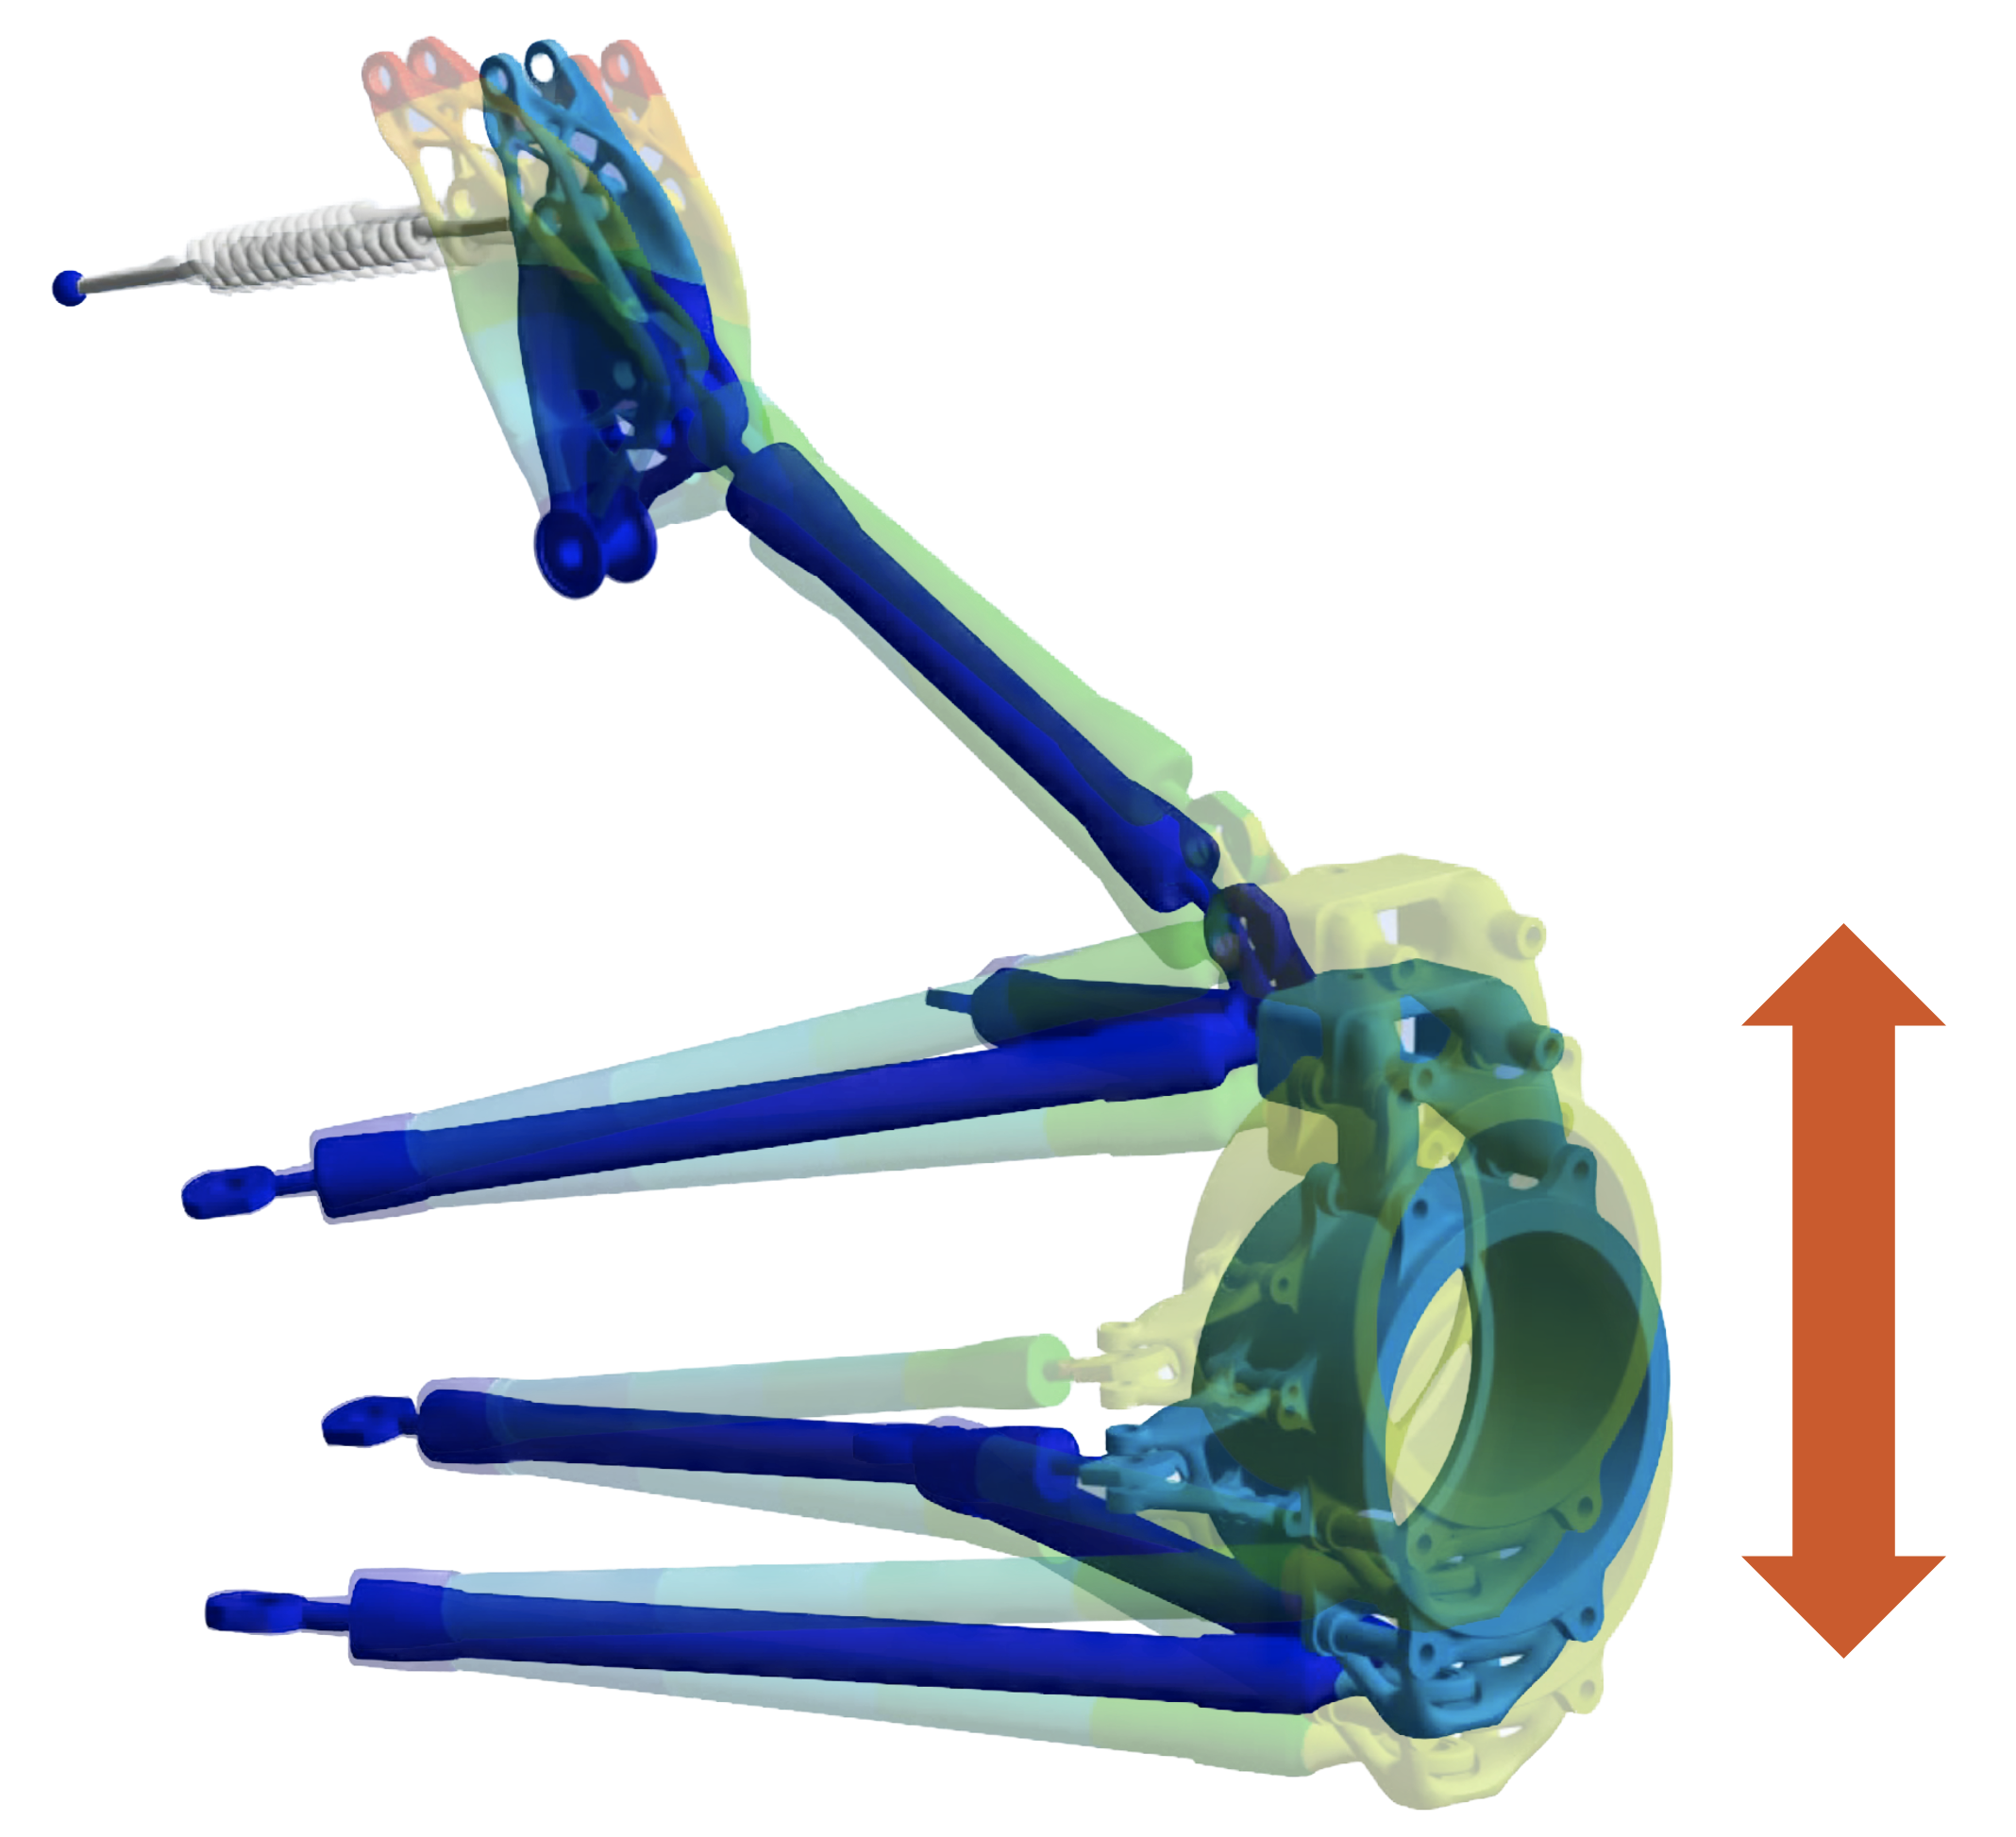
\includegraphics[width=1.0\linewidth]{figures/chapter_4/suspension_mode_1}
    \caption{$f_1 = \SSI{7.6}{\hertz}$}
  \end{subfigure}
  \begin{subfigure}[c]{0.225\textwidth}
    \centering
    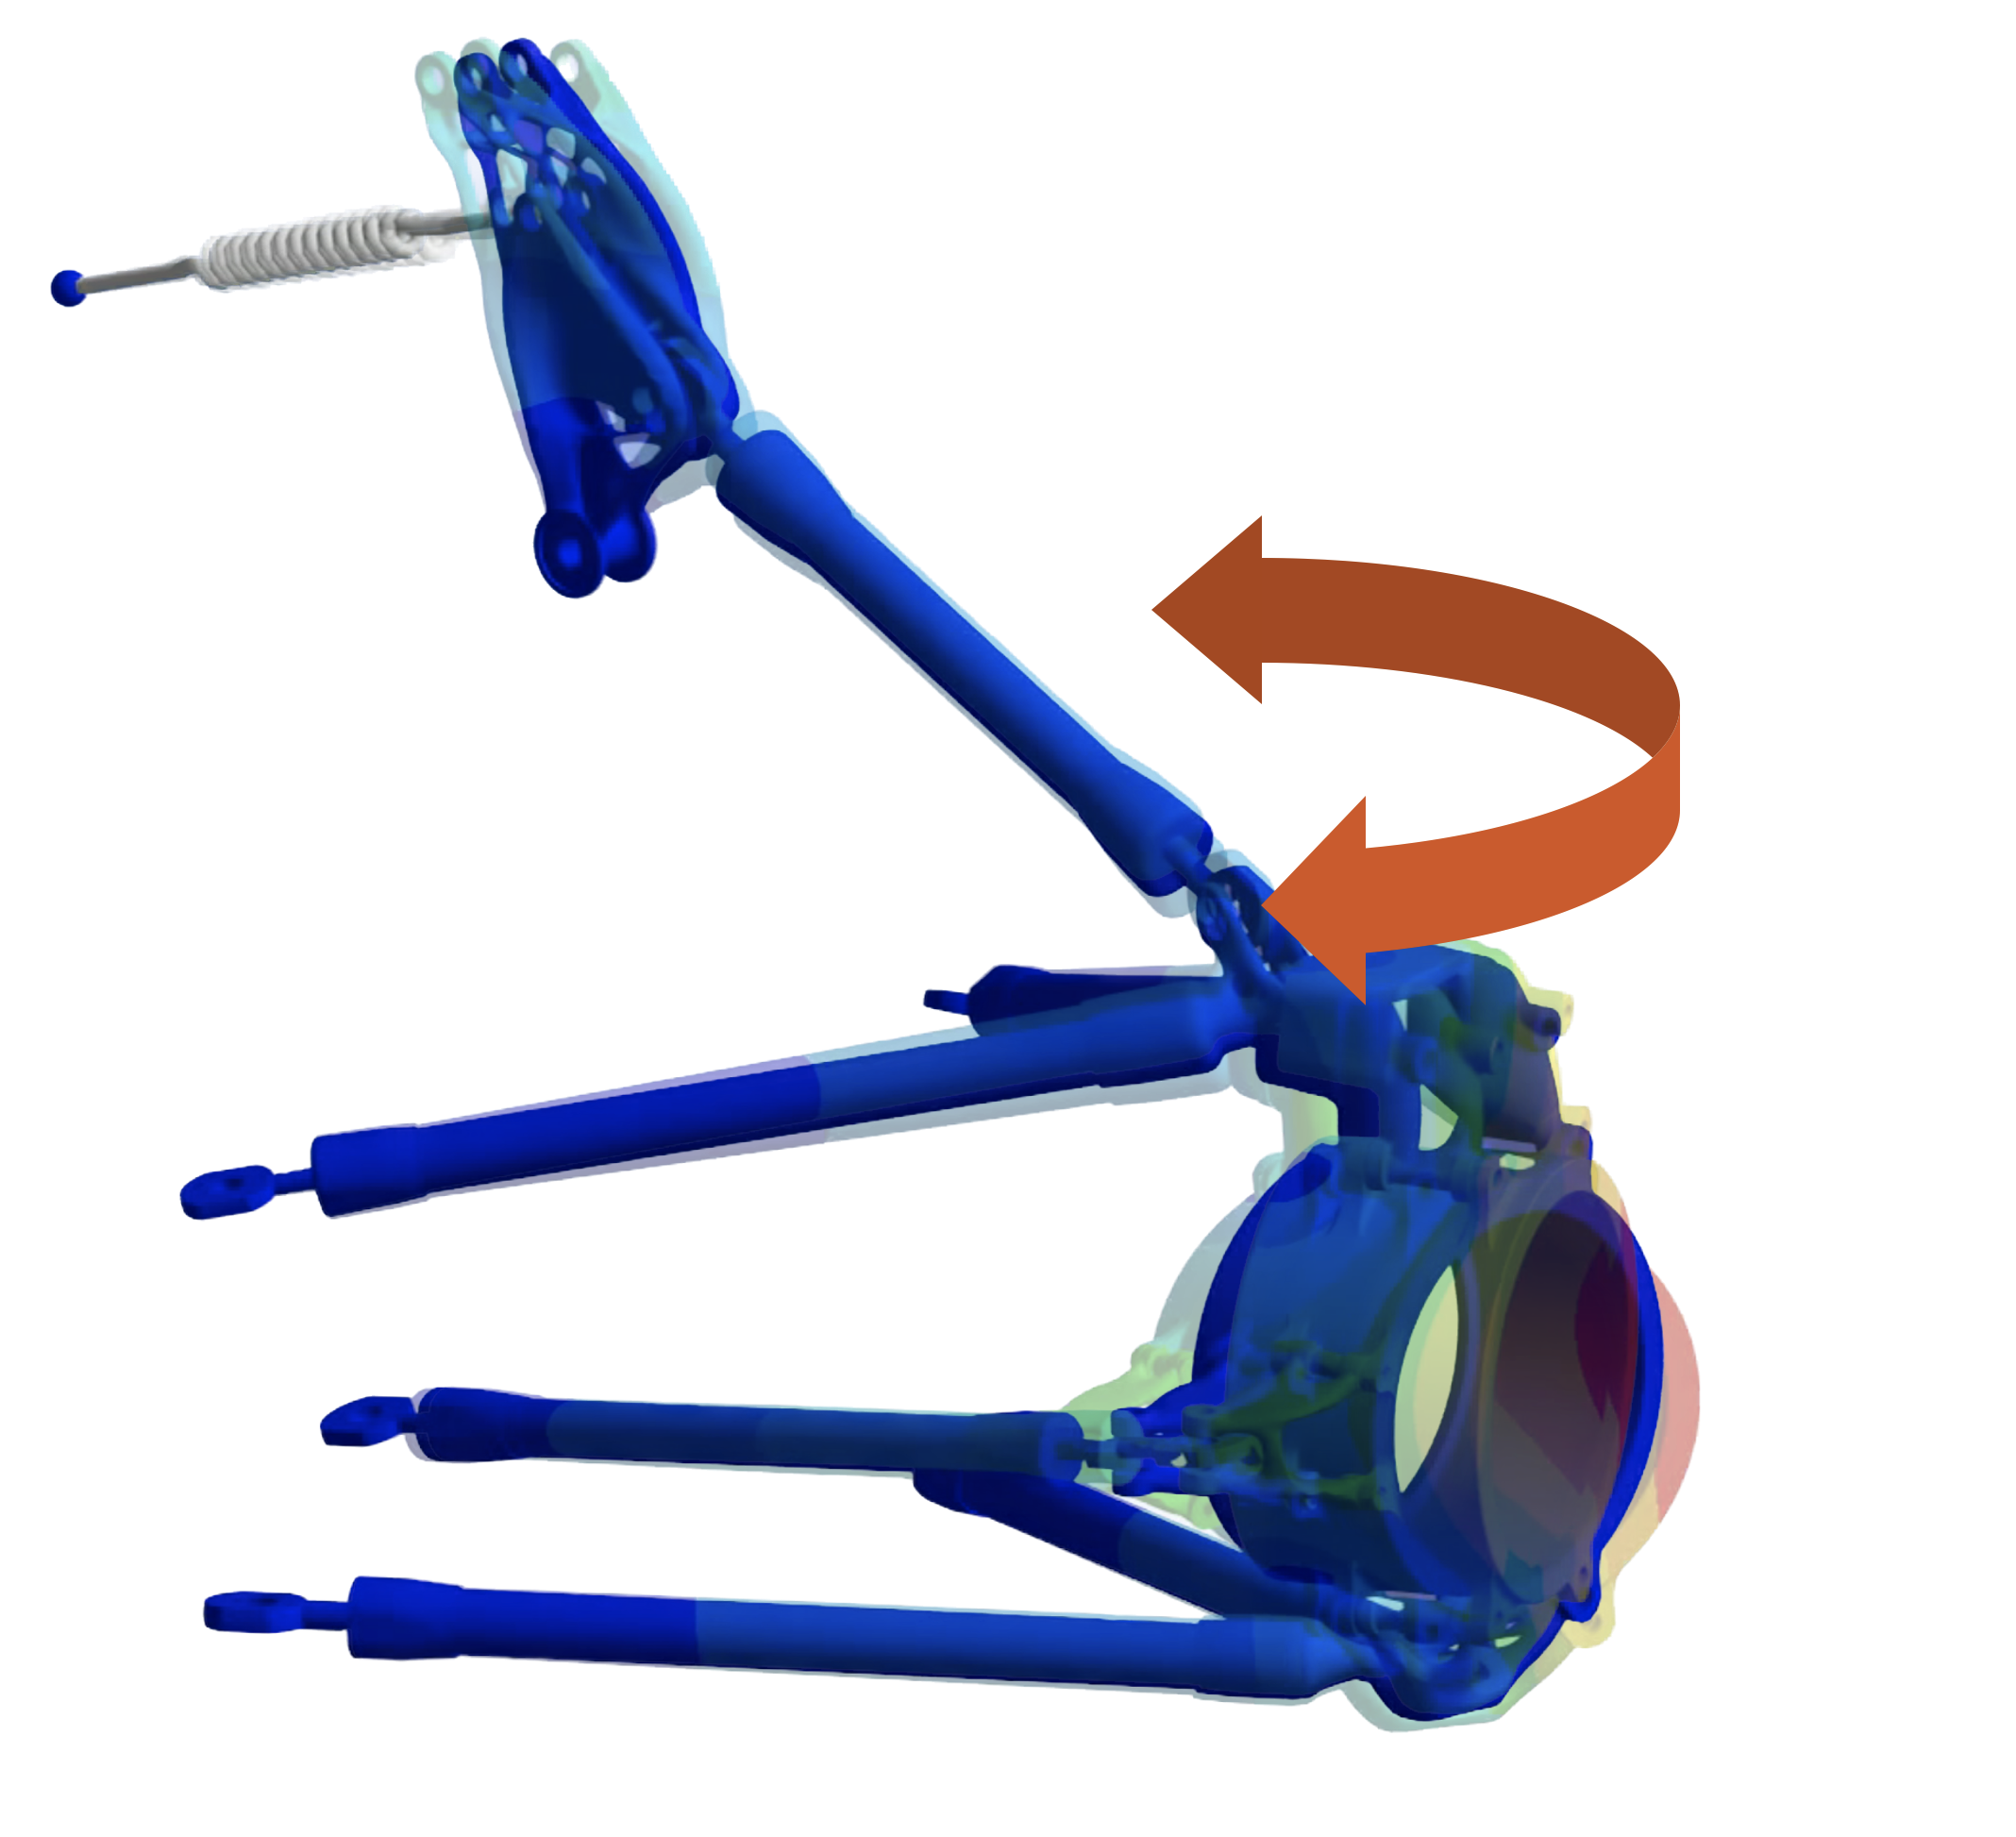
\includegraphics[width=1.0\linewidth]{figures/chapter_4/suspension_mode_2}
    \caption{$f_2 = \SSI{88.5}{\hertz}$}
  \end{subfigure}
  \begin{subfigure}[c]{0.225\textwidth}
    \centering
    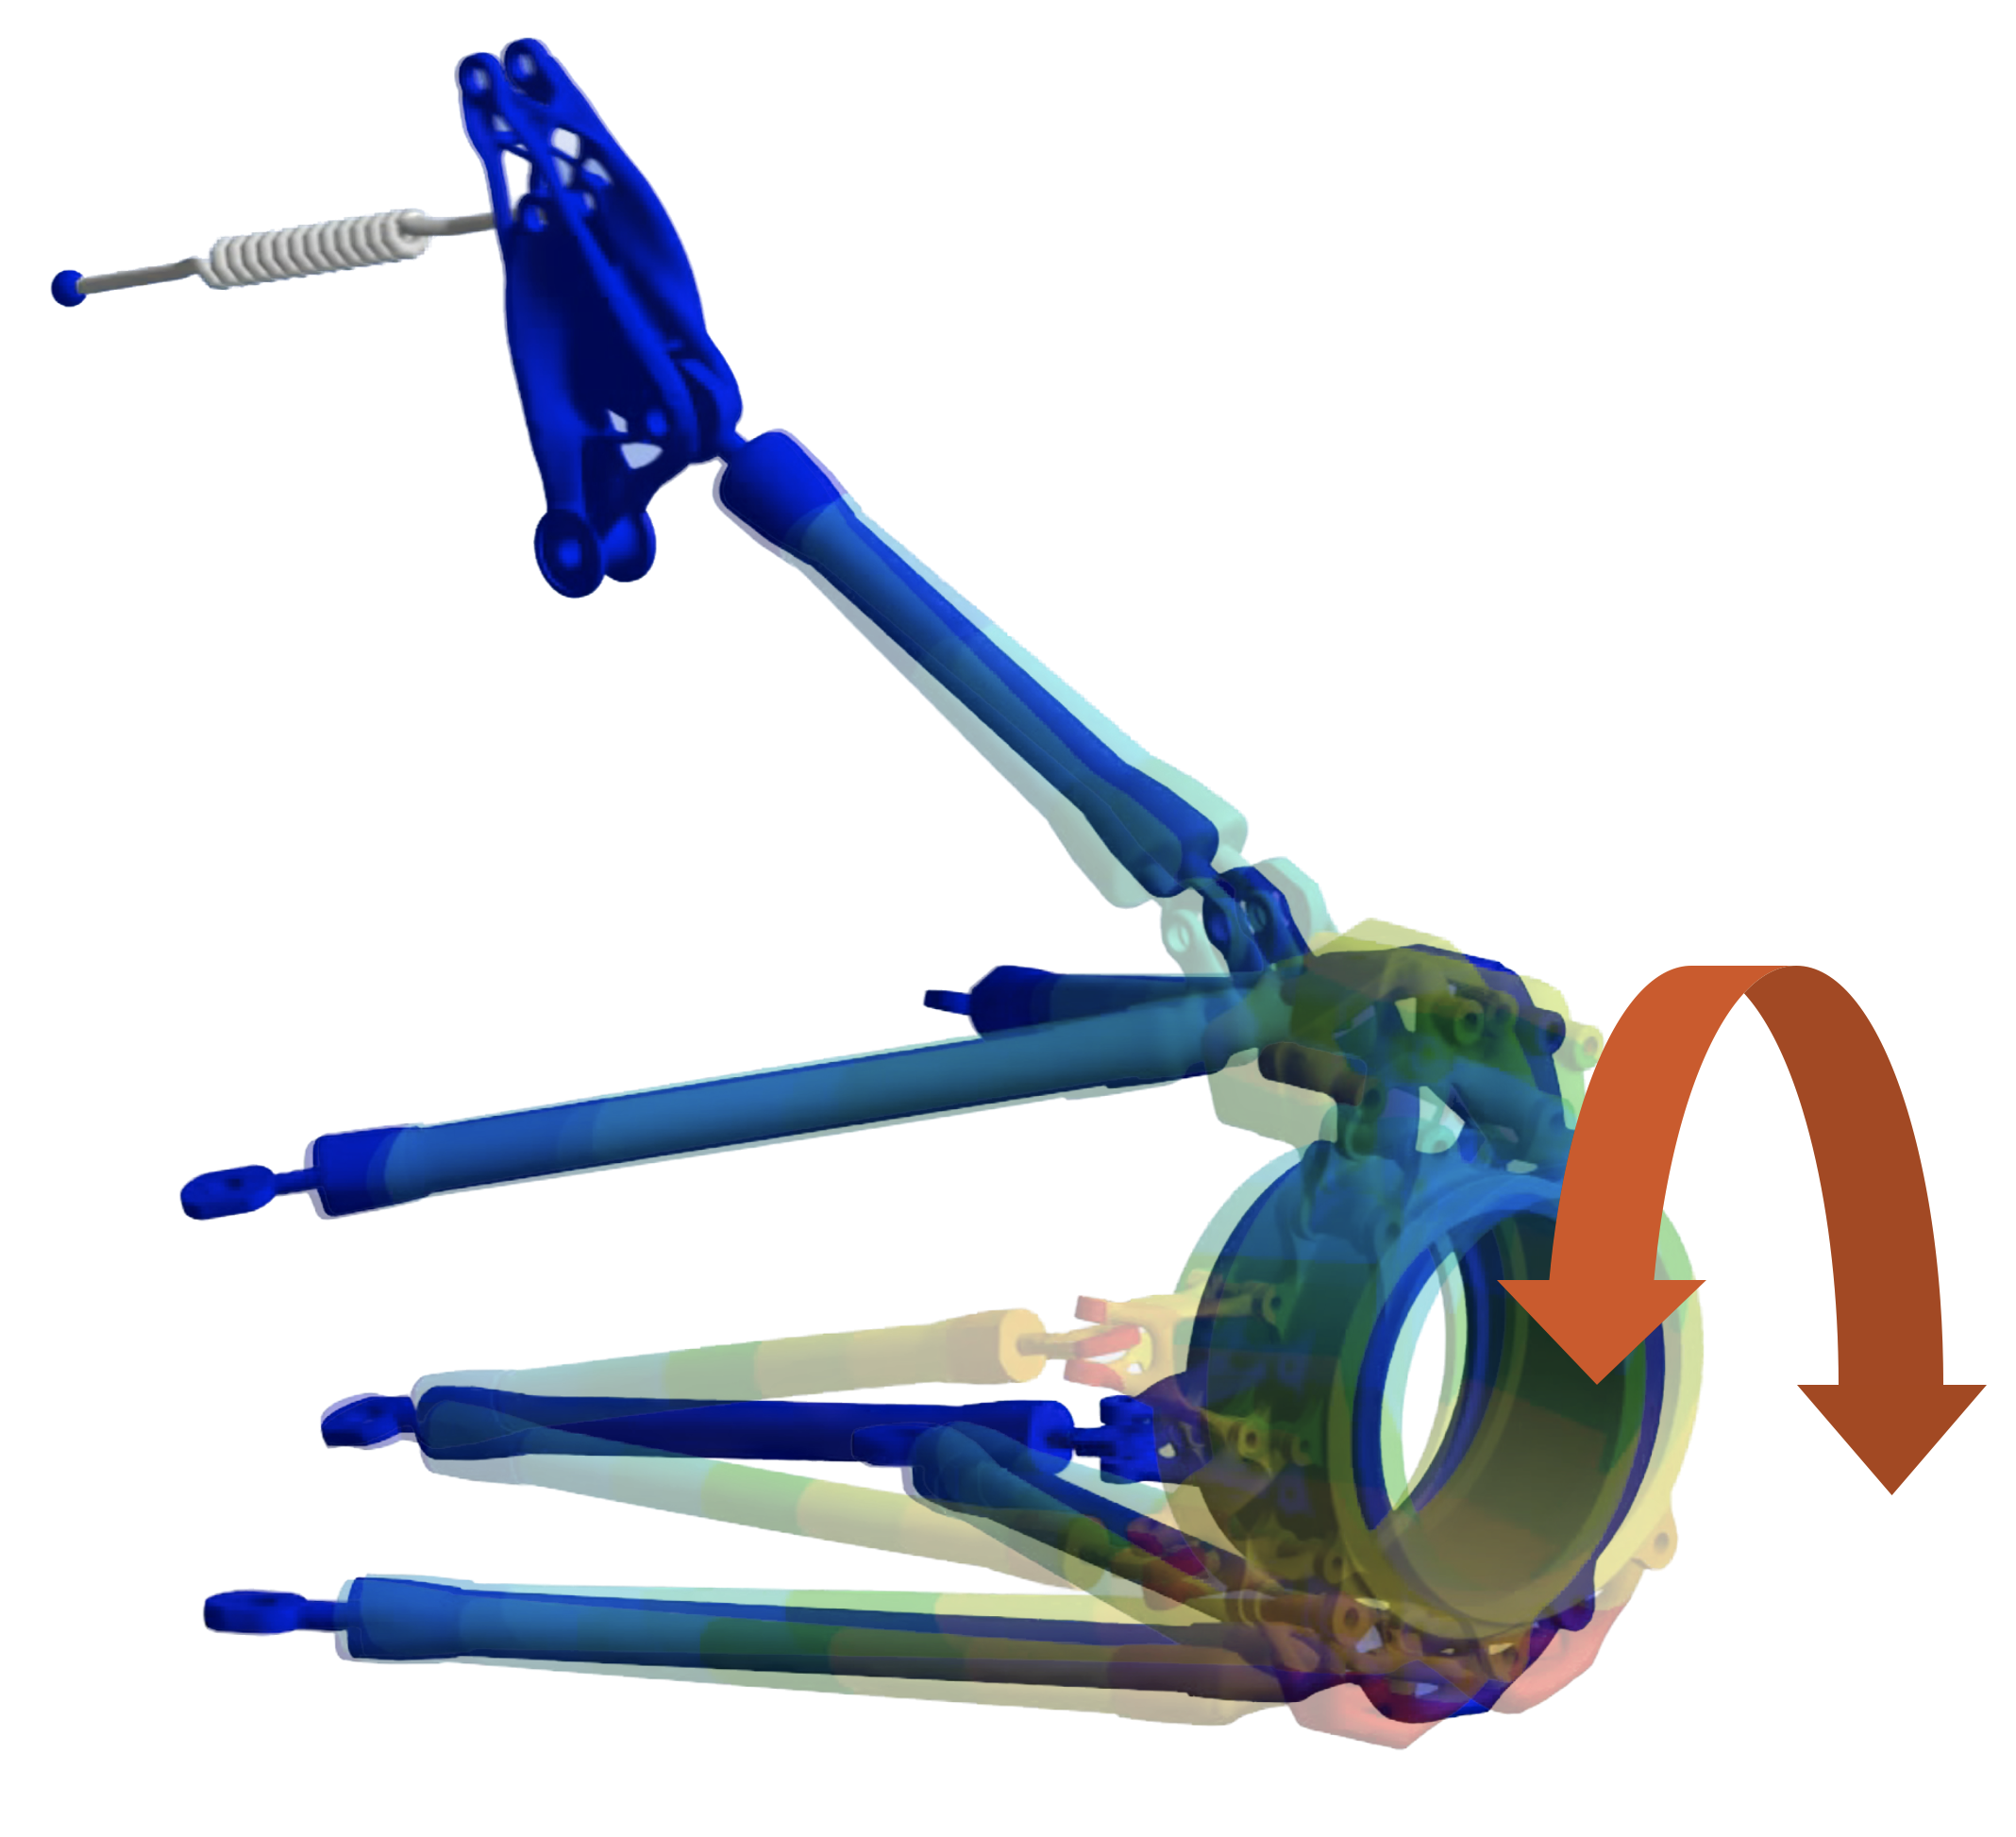
\includegraphics[width=1.0\linewidth]{figures/chapter_4/suspension_mode_3}
    \caption{$f_3 = \SSI{159.7}{\hertz}$}
  \end{subfigure}
  \caption{First three modal shapes of the suspension.}
  \label{chap5:fig:suspension_modes}
\end{figure}

\begin{figure}[htbp]
  \centering
  \small{\includetikz{figures/chapter_4/suspension_dynamic_deformations.tex}}
  \caption{Frequency response analysis of the suspension model is conducted, with tests performed under the equilibrium between the suspension system and a vertical force of \SI{500}{\newton} applied at the wheel hub. Frequency responses are assessed by applying input forces/torques at the wheel hub in the form of a linear chirp spanning frequencies from \SIrange{0}{200}{\hertz}, with a constant amplitude of \SI{5}{\newton}/\SI{5}{\newton\meter}. \emph{Legend:} {\color{mycolor1}$\blacksquare$} \Simulink{} multi-body simulation with full compliance dynamics contribution, {\color{mycolor2}$\blacksquare$} \Simulink{} multi-body with steady-state compliance contribution, {\color{mycolor3}$\blacksquare$} \Ansys{} \ac{FE} modal analysis.}
  \label{chap5:fig:suspension_dynamic_results}
\end{figure}

The reduced system is then used to perform a transient analysis of the suspension system, coupled with the tire-ground enveloping model and the tire model presented in Appendix~\ref{app2:enve} (supported by the \Acme{} \cpp{} library described in Appendix~\ref{app1:acme}) and Appendix~\ref{app3:tirex}, respectively. The transient analysis is conducted to understand the impact of compliance on the vehicle dynamics as well as suspension rods' diameter in the development of tire-ground forces. A side slip angle ramp simulation is thus performed to evaluate the effect of suspension compliance on the lateral force of the tire. For this simulation, the following four cases are analyzed:
%
\begin{itemize}
  \setlength\itemsep{0.0em}
  \item pure kinematic suspension model;
  \item kinematic and nominal compliance model;
  \item kinematic and compliance model with $-10\%$ suspension rods diameter;
  \item kinematic and compliance model with $-20\%$ suspension rods diameter.
\end{itemize}
%
The results of the simulation are shown in Figure~\ref{chap5:fig:test_bench}, which compares the four cases. The lateral force $F_y$ is depicted with solid lines, while the difference between the lateral force of the pure kinematic simulation and the other cases is illustrated in dashed lines. The displayed curves show a non-negligible effect of suspension compliance on the lateral force of the tire is observed. As expected, the larger difference in the generated $F_y$ force can be observed in the linear region of the tire slip characteristic curve, where the slip cornering stiffness is higher. The difference then decreases as the peak approaches. Further observations could be made on the impact of these findings on the vehicle dynamics and handling. However, this is beyond the scope of this work.

\begin{figure}[!htp]
  \centering
  \small{\includetikz{figures/chapter_4//test_bench.tex}}
  \caption{Tire lateral force $F_y$ during a side slip angle ramp simulation. Solid lines represent the results obtained with the \Simulink{} model, while dashed lines represent the difference between the various simulations (see legend below). \emph{Solid lines legend:}
  {\color{mycolor1}\raisebox{-.15pt}{$\blacksquare$}} kinematics, {\color{mycolor2}\raisebox{-.15pt}{$\blacksquare$}} kinematics and compliance, {\color{mycolor3}\raisebox{-.15pt}{$\blacksquare$}} kinematics and compliance ($-10\%$ rods diameter), {\color{mycolor5}\raisebox{-.15pt}{$\blacksquare$}} kinematics and compliance ($-20\%$ rods diameter).   \emph{Dashed lines legend:} {\color{mycolor1}\raisebox{-.15pt}{\scalebox{0.5}[1.0]{$\blacksquare$}}}{\color{mycolor2}\raisebox{-.15pt}{\scalebox{0.5}[1.0]{$\blacksquare$}}} = {\color{mycolor1}\raisebox{-.15pt}{$\blacksquare$}} $-$ {\color{mycolor2}\raisebox{-.15pt}{$\blacksquare$}}, {\color{mycolor1}\raisebox{-.15pt}{\scalebox{0.5}[1.0]{$\blacksquare$}}}{\color{mycolor3}\raisebox{-.15pt}{\scalebox{0.5}[1.0]{$\blacksquare$}}} = {\color{mycolor1}\raisebox{-.15pt}{$\blacksquare$}} $-$ {\color{mycolor3}\raisebox{-.15pt}{$\blacksquare$}},  {\color{mycolor1}\raisebox{-.15pt}{\scalebox{0.5}[1.0]{$\blacksquare$}}}{\color{mycolor5}\raisebox{-.15pt}{\scalebox{0.5}[1.0]{$\blacksquare$}}} = {\color{mycolor1}\raisebox{-.15pt}{$\blacksquare$}} $-$ {\color{mycolor5}\raisebox{-.15pt}{$\blacksquare$}}.
  }
  \label{chap5:fig:test_bench}
\end{figure}

Finally, to estimate what would be the impact of compliance in a racing vehicle, the telemetry and inputs of a full-vehicle simulation conducted on the \textit{Pista Azzurra} track in Jesolo (Italy), are applied to the modeled rear left double wishbone suspension. The simulation is conducted using the previously reduced \ac{MB}-\ac{DAE} system, the tire-ground enveloping model, and the tire model presented in Appendices~\ref{app2:enve} and~\ref{app3:tirex}, respectively. The results of the simulation are shown in Figure~\ref{chap5:fig:suspension_pista_azzurra}, where the suspension travel $z$ is shown in the first plot, while the translations $\delta$ and rotation $\theta$ components of the compliance contribution at the wheel hub are shown in the second and third plots, respectively. The results show that the compliance of the suspension system adds a non-negligible contribution to the wheel hub's positioning, especially in terms of rotations.

\begin{figure}[htbp]
  \centering
  \small{\includetikz{figures/chapter_4/suspension_pista_azzurra.tex}}
  \caption{Simulation of the rear left double wishbone suspension of the Formula SAE \textit{E-Agle Trento Racing Team} vehicle~\cite{eagle} on the \textit{Pista Azzurra} track in Jesolo (Italy). The simulation is conducted using the index-reduced \ac{DAE} system, the tire-ground enveloping model, and the tire model presented in Appendices~\ref{app2:enve} and~\ref{app3:tirex}, respectively. In the first plot, the suspension travel $z$ is shown, while the second and third plots show the translations $\delta$ and rotation $\theta$ components of the compliance contribution at the wheel hub. \emph{Legend}: {\color{mycolor1}$\blacksquare$} $x$-axis component, {\color{mycolor2}$\blacksquare$} $y$-axis component, {\color{mycolor3}$\blacksquare$} $z$-axis component.}
  \label{chap5:fig:suspension_pista_azzurra}
\end{figure}

\section{Trajectory Prescribed Path Control}
\label{chap5:sec:tppc}

The \ac{TPPC} category is characterized by \ac{DAE} systems that describe the motion of a dynamical system whose trajectory is prescribed by adding a set of path constraints to the equations of motion. The model equations evolve into a non-linear semi-explicit \acp{DAE}. Within this system, the differential equations represent motion equations, while the algebraic equations correspond to imposed path constraints, collectively constituting \ac{TPPC} problems. Historically, addressing specific \ac{TPPC} challenges involved the development of software models that promptly adjust control variables to approximate prescribed path profiles. In this context, we investigate general numerical techniques directly applicable to \acp{DAE}. \ac{TPPC} problems are present in various fields, such as robot control, chemical process management, as well as space vehicle and aircraft guidance.

The \ac{DAE} systems arising from \ac{TPPC} simulations has typically the Hessenberg form~\cite{brenan1986numerical}
%
\begin{equation*}
  \begin{cases}
    \m{x}^\prime = \m{f}(\m{x}, \m{u}, t) & \text{differential equations} \\
    \m{0}        = \m{g}(\m{x}, \m{u}, t) & \text{path constraints}
  \end{cases} \, \text{,}
  \quad \text{with} \quad \jac{\m{g}}{\m{x}} \, \jac{\m{f}}{\m{u}} ~ \text{non-singular}
  \label{chap5:eq:tppc_dae_index2}
\end{equation*}
%
for index-2 problems, and
%
\begin{equation*}
  \begin{cases}
    \m{x}^\prime = \m{f}(\m{x}, \m{y}, \m{u}, t) \\
    \m{y}^\prime = \m{g}(\m{x}, \m{y}, t) \\
    \m{0}        = \m{h}(\m{y}, t)
  \end{cases} \, \text{,}
  \quad \text{with} \quad \jac{\m{h}}{\m{y}} \, \jac{\m{g}}{\m{x}} \, \jac{\m{f}}{\m{u}} ~ \text{non-singular}
  \label{chap5:eq:tppc_dae_index3}
\end{equation*}
%
for index-3 problems. The index of such systems is typically higher than the non-controlled counterpart. Indeed, the path constraints control is embedded in the state equations, often increasing the length of the differentiation chain to obtain a set of \acp{ODE}. Specifically, when the Jacobian $\jac{\m{g}}{\m{u}}$ is non-singular, the path equations are commonly referred to as control variable constraints and the corresponding \acp{DAE} has index-1. It is not uncommon to find that the path constraints in a \ac{TPPC} problem are functions only of the differential variables so that $\jac{\m{g}}{\m{u}} = \m{0}$ and the \acp{DAE} will be of higher index~\cite{brenan1995numerical}. To showcase the capabilities of the proposed index reduction algorithm in handling such high-index \ac{TPPC} problems, different examples are presented. Two problems regarding the initial and final phases of the space shuttle reentry, described by index-2 and index-3 \acp{DAE}~\cite{brenan1995numerical}. Lastly, one problem on the control of a robotic arm, which is described as a complicated index-5 system~\cite{pryce1998solving}. A brief discussion of each of these examples, together with an introduction to the application field, is presented in the following sections.

\subsection{Space Shuttle Reentry Problems}

In space applications, \ac{TPPC} problems aid in vehicle performance analysis during design, particularly for lifting reentry vehicles aiming to determine maximum crossrange (or downrange) capability. Trajectory profiles are constrained by skin temperature limits set by the thermal protection design. \ac{OC} theory offers a direct approach to addressing maximum crossrange capability with heating constraints, formulated as a two-point boundary value problem involving \acp{DAE} and adjoint variables. However, solving such \acp{OCP} requires starting solutions close to the optimal, especially with heating constraints, due to extreme sensitivity to initial guesses in shooting problems. An indirect \ac{TPPC} approach or using \ac{TPPC} to generate initial solutions for \ac{OC} may offer more success. Typically, maximizing crossrange capability involves holding the angle of attack $\alpha$ near the maximum lift/drag value, often set at around \SI{40}{\deg} in \ac{NASA} space shuttle reentry simulations, leaving bank angle $\beta$ adjustments to satisfy remaining functional constraints. In certain scenarios, varying system parameters can effectively optimize vehicle crossrange capability by ensuring trajectory adherence to specific constraints, thereby presenting a semi-explicit non-linear \acp{DAE} \ac{TPPC} problem~\cite{brenan1986numerical, brenan1995numerical}.

The discussion is confined to a reentry vehicle in the absence of propulsive forces, where we simplify the simulation to model solely spherical geopotential and spherical earth. The equations of motion in relative coordinates are thus expressed as follows
%
\begin{equation}
  \begin{cases}
  H^{\prime}       = V_r\sin(\gamma) \\
  \xi^{\prime}     = \dfrac{V_r\cos(\gamma) \sin(A)}{r \cos(\lambda)} \\
  \lambda^{\prime} = \dfrac{V_r}{r} \cos(\gamma) \cos(A) \\
  V_r^{\prime}     = -\dfrac{D}{m} - g\sin(\gamma) - \Omega_e^2 r \cos(\lambda)(\sin(\lambda) \cos(A) \cos(\gamma)-\cos(\lambda) \sin(\gamma)) \\
  \gamma^{\prime}  = \dfrac{L\cos(\beta)}{m V_r}+\dfrac{\cos(\gamma)}{V_r}\left(\dfrac{V_r^2}{r}-g\right) + 2\Omega_e \cos(\lambda) \sin(A)\dots \\
  \qquad + \dfrac{\Omega_e^2 r \cos(\lambda)}{V_r}(\sin(\lambda) \cos(A) \sin(\gamma)+\cos(\lambda) \cos(\gamma)) \\
  A^{\prime}       = \dfrac{L\sin(\beta)}{m V_r \cos(\gamma)}+\dfrac{V_r}{r} \cos(\gamma) \sin(A) \tan(\lambda) - 2\Omega_e(\cos(\lambda) \cos(A) \tan(\gamma) - \sin(\lambda)) \dots \\
  \qquad + \dfrac{\Omega_e^2 r \cos(\lambda) \sin(\lambda) \sin(A)}{V_r \cos(\gamma)}
  \end{cases} \, \text{,}
  \label{chap5:eq:space_shuttle_reentry}
\end{equation}
%
where the state variables are $\m{x} = [H, \xi, \lambda, V_r, \gamma, A]^\top$. The parameters are the following
%
\begin{equation*}
  \begin{aligned}
    r           & = H + r_e, & \text{distance from the earth center,} \\
    r_e         & = \SI{20902900}{\feet} & \text{earth radius,} \\
    g           & = \mu/r^2 & \text{gravity force,} \\
    \mu         & = \SI{1.407653916\times 10^16}{\cubic\feet\per\second\squared} & \text{gravitational constant,} \\
    \Omega_e    & = \SI{360/(24\cdot60\cdot60)}{\deg\per\second} & \text{earth angular speed,} \\
    \rho(H)     & = 0.002378\exp(-H/23800) & \text{atmospheric density,} \\
    L(V_r)      & = 1/2 \rho C_L S V_r^2 & \text{aerodynamic lift force,} \\
    D(V_r)      & = 1/2 \rho C_D S V_r^2 & \text{aerodynamic drag force.}
  \end{aligned}
\end{equation*}
%
The aerodynamic lift and drag coefficients, respectively $C_L(\alpha)$ and $C_D(\alpha)$, as well as the vehicle cross-sectional area $S$ and mass $m$, will be later specified on the specific test. The control variables, which dictate both the magnitude and direction of the aerodynamic force applied to the vehicle, are assessed within the body coordinate system (refer to Figure~\ref{chap5:fig:shuttle_frame}). The bank angle $\beta$ corresponds to a rotation or \emph{roll} about the vehicle's $x$-axis, while the angle of attack $\alpha$ is measured from the relative velocity vector of the vehicle to the body $x$-axis, representing a rotation or \emph{pitch} about the body $y$-axis. For a more detailed explanation of these parameters and the coordinate system on the presented tests, please refer to~\cite{brenan1983stability}. Nonetheless, figure~\ref{chap5:fig:shuttle_reentry} illustrates the space shuttle coordinate system, as well as the vehicle's position with respect to the earth reference frame.

\begin{figure}[htb]
  \centering
  \begin{subfigure}[c]{0.475\textwidth}
    \centering
    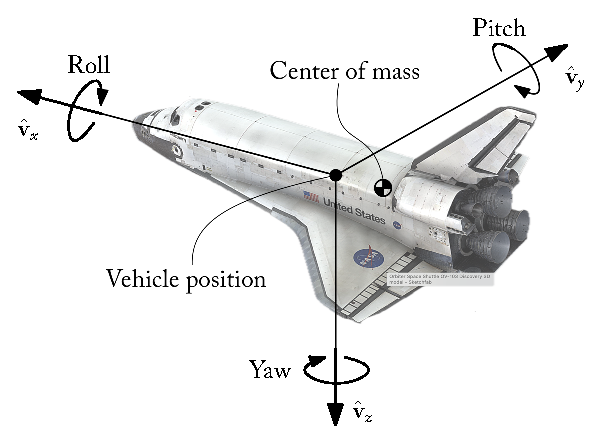
\includegraphics[width=1.0\linewidth]{figures/chapter_4/shuttle_frame.eps}
    \caption{Space shuttle reentry vehicle coordinate system.}
    \label{chap5:fig:shuttle_frame}
  \end{subfigure}%
  \hfill
  \begin{subfigure}[c]{0.475\textwidth}
    \centering
    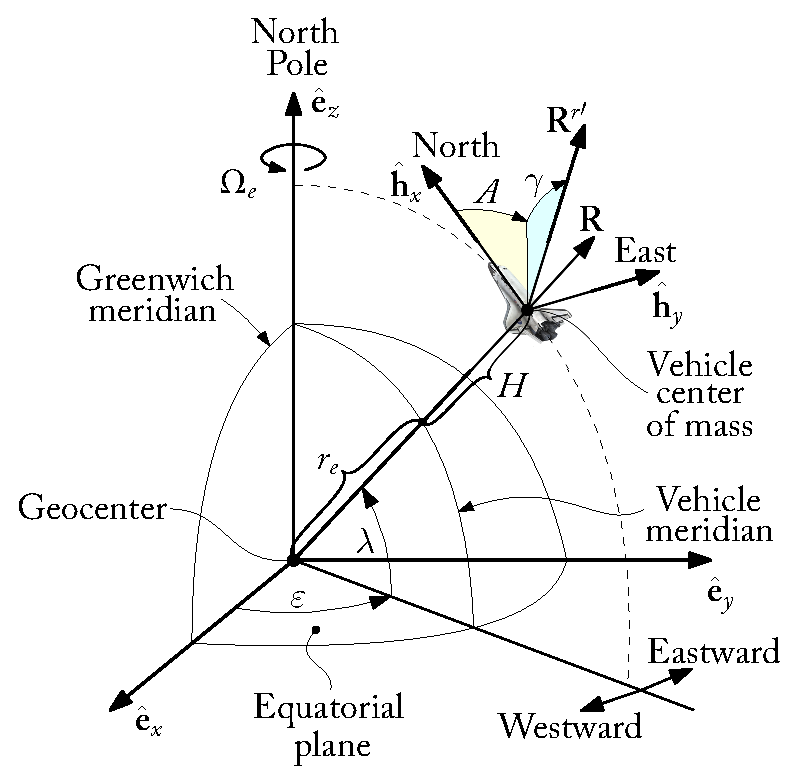
\includegraphics[width=1.0\linewidth]{figures/chapter_4/earth_frame.eps}
    \caption{Earth reference frame.}
    \label{chap5:fig:earth_frame}
  \end{subfigure}
  \caption{Coordinate systems for the space shuttle reentry problem~\cite{brenan1995numerical, brenan1986numerical}.}
  \label{chap5:fig:shuttle_reentry}
\end{figure}

Once the space shuttle concludes its mission in space, it must return to Earth for landing, subject to various mission constraints, such as heating limitations to prevent vehicle damage. Instead of directly imposing these heating constraints as algebraic limitations, an alternative approach involves prescribing a nominal drag acceleration versus a relative velocity profile. This profile is selected to ensure that temperature constraints are satisfied as long as the vehicle follows a trajectory complying with this drag constraint. During reentry, the standard equations of motion~\eqref{chap5:eq:space_shuttle_reentry} are compounded with an algebraic constraint representing the drag acceleration profile, forming a \ac{DAE} system. Typically, the angle of attack remains constant or is only slightly varied, while the bank angle serves as the control variable. In the following, we examine the initial and final phases of reentry. The first involves maneuvering the vehicle from a given state to one lying on the nominal drag constraint. While the second entails flying the vehicle along the nominal drag constraint.

\subsubsection{Initial Stage Reentry Problem}

We now examine the initial stage reentry \ac{TPPC} problem in the same form of~\cite{brenan1986numerical}. This problem is part of a broader trajectory optimization process aimed at determining a surface of admissible reentry states. Following completion of on-orbit maneuvers, the vehicle must transition to a state vector enabling safe flight to the landing site. This set of allowable states is denoted as a target line. A given initial state qualifies as a target line point if a trajectory can be executed from that state in such a way that the vehicle's drag versus relative velocity profile smoothly aligns with the specified nominal profile, without overshooting and thus without violating any temperature constraints. Consider now the description of the vehicle's drag acceleration versus relative velocity profile, expressed as
%
\begin{equation}
  \dfrac{D}{m} - (C_0 + C_1 (V_r - V_0) + C_2 (V_r - V_0)^2 + C_3 (V_r - V_0)^3) = 0 \, \text{,}
  \label{chap5:eq:initial_drag}
\end{equation}
%
for a time $t \in [t_0, t_1] = \RSI{32.868734542}{419.868734542}{\second}$, and where $V_0$, is the vehicle's initial velocity at $t_0$ and $C_0 = 3.974960446019$, $C_1 = -0.01448947694635$, $C_2 = -0.2156171551995 \cdot 10^{-4}$, and $C_3 = -0.1089609507291 \cdot 10^{-7}$ are constants chosen so that the initial state vector satisfies~\eqref{chap5:eq:initial_drag} and its first derivative at $t_0$, and so that this transitional phase smoothly joins with the nominal profile. Notice that, posed in this way, the resulting \ac{TPPC} system is a semi-explicit index-3 \acp{DAE} problem. In this test, the set of initial values are $\gamma = \SI{-0.749986488}{\deg}$, $A = \SI{62.7883367}{\deg}$, $H = \SI{264039.3280}{\feet}$, $\xi = \SI{177.718047}{\deg}$, $\lambda = \SI{32.0417885}{\deg}$, $V_r = \SI{24317.0798}{\feet\per\second}$, and $\beta = \SI{41.10071834}{\deg}$. The lift and drag coefficients $C_L = 0.8769230769$ and $C_D = 0.8246153846$, as well as the angle of attack $\alpha = \SI{40}{\deg}$ are assumed to be constant throughout the simulation. The vehicle mass is $m = \SI{5964.496499824}{\slugs}$, and its cross-sectional reference area is $S = \SI{2690}{\feet\squared}$.

\begin{table}
  \caption{Expression complexity encountered throughout the index reduction of the initial stage space shuttle reentry problem~\cite{brenan1995numerical} \ac{DAE} system. \emph{Legend}: $\cf$ = functions, $\ca$ = additions, $\cm$ = multiplications, and $\cd$ = divisions.}
  \label{chap5:tab:tppc_initial}
  \centering
  {\footnotesize\begin{tabular}{cccc}
    \multicolumn{4}{c}{\textbf{Initial Stage Space Shuttle Reentry Problem~\cite{brenan1995numerical}}} \\
    \toprule
    \textbf{Original \acp{DAE}} & \multicolumn{3}{c}{$\mF = 153\cf + 2\cd + 275\cm + 59\ca$ \quad $\mh = 0$} \\
    \midrule
    \textbf{Reduction step} & $\mE$ & $\mg$ & $\ma$ \\
    \midrule
    Index-3 \acp{DAE} & $11\cf + 9\cm + 5\ca$ & $118\cf + 1\cd + 220\cm + 36\ca$ & $6\cf + 1\cd + 28\cm + 10\ca$ \\
    Index-2 \acp{DAE} & $11\cf + 9\cm + 5\ca$ & $118\cf + 1\cd + 220\cm + 36\ca$ & $81\cf + 2\cd + 472\cm + 87\ca$ \\
    Index-1 \acp{DAE} & $11\cf + 9\cm + 5\ca$ & $118\cf + 1\cd + 220\cm + 36\ca$ & $567\cf + 3\cd + 6198\cm + 888\ca$ \\
    Index-0 \acp{DAE} & $4053\cf + 24\cd + 41102\cm + 5792\ca$ & $118\cf + 1\cd + 220\cm + 36\ca$ & $0$ \\
    \midrule
    \textbf{Reduced \acp{DAE}} & \multicolumn{3}{c}{$\mF = 3075\cf + 4\cd + 34811\cm + 4734\ca$ \quad $\mh = 654\cf + 6\cd + 6698\cm + 985\ca$} \\
    \bottomrule
  \end{tabular}}
\end{table}

To address this index-3 \acp{DAE}, we utilize the proposed index reduction algorithm. The complexity of expressions encountered during the algorithm's execution is detailed in Table~\ref{chap5:tab:tppc_initial}. Notably, the index reduction algorithm effectively reduced the system to index-0 without the aid of hierarchical representations, and the expression growth is strongly inhibited by successful simplification and only limited to the last reduction step. We conduct numerical integration of the reduced \ac{DAE} system using both the \Maple{} and \Indigo{} solvers. Specifically, \Maple{} encounters challenges in integrating the original \ac{DAE} system due to difficulties in projecting initial values into the solution space, where \acp{IC} are deemed inconsistent with the algebraic constraints. In contrast, the \Indigo{} numerical solver successfully integrates the reduced \ac{DAE} system, yielding results depicted in Figure~\ref{chap5:fig:tppc_initial}.

\begin{figure}[htb]
  \centering
  \small{\includetikz{figures/chapter_4/shuttle_index3_control.tex}}
  \caption{Control history of the initial stage space shuttle reentry problem~\cite{brenan1995numerical}. The vehicle's trajectory is prescribed by the drag acceleration $D/m$ versus a relative velocity $V_r$ profile reported in~\eqref{chap5:eq:initial_drag}. The vehicle's state is controlled by the bank angle $\beta$ and the angle of attack is kept fixed at $\alpha = \SI{40}{\deg}$. \emph{Legend}: \textcolor{mycolor1}{$\blacksquare$} bank angle $\beta$, and \textcolor{mycolor2}{$\blacksquare$} angle of attack $\alpha$.}
  \label{chap5:fig:tppc_initial}
\end{figure}

\subsubsection{Final Stage Reentry Problem}

We now examine the final stage reentry \ac{TPPC} problem in the same form of~\cite{brenan1995numerical}. Let us assume the objective is to navigate a vehicle along a predetermined azimuth $A$ and flight path angle trajectory $\gamma$, as defined by the constraints on state variables
%
\begin{equation}
  \gamma + 1 + 9\left(\dfrac{t}{300}\right)^2 = 0 \, \text{,}
  \qquad \text{and} \qquad
  A - 45 + 90\left(\dfrac{t}{300}\right)^2 = 0 \, \text{.}
  \label{chap5:eq:final_path_constraints}
\end{equation}
%
for a time $t \in \RSI{0}{300}{\second}$. The flight path angle $\gamma$ spans from $\RSI{-1}{-10}{\deg}$, while the azimuth $A$ ranges from $\RSI{45}{135}{\deg}$. Both the bank angle $\beta$ and the angle of attack $\alpha$ serve as control variables, \ie{} $\m{u} = [\beta, \alpha]^\top$. The \ac{DAE} system is index-2 for a lifting reentry vehicle as long as $(0.05 \rho S V_r/m)^2 C_L(\alpha)/\cos(\gamma) \neq 0$. Notice that to be physically consistent we require that $V_r \neq \SI{0}{\deg}$, $\rho\neq \SI{0}{\deg}$, $\alpha \neq \SI{0}{\deg}$, $\gamma \neq \SI{90}{\deg}$, as well as $\lambda \neq \SI{180}{\deg}$. The related index-1 \acp{DAE} can be obtained directly by differentiating the algebraic constraints once and substituting for $A^\prime$ and $\gamma^\prime$ from the differential equations. Consistent initial values for the \ac{DAE} system are determined by selecting the initial differential and control variables to satisfy~\eqref{chap5:eq:final_path_constraints} the two new hidden constraints in the related index-1 system. The set of initial values used in this experiment are $H = \SI{100000}{\feet}$, $\xi = \SI{0}{\deg}$, $\lambda = \SI{0}{\deg}$, $A = \SI{0}{\deg}$, $V_r = \SI{12000}{\feet\per\second}$, $\gamma = \SI{-1}{\deg}$, $A = \SI{45}{\deg}$, $\beta = \SI{-0.05220958616134}{\deg}$, and $\alpha = \SI{2.6728700742}{\deg}$. The lift and drag coefficients are set to $C_L = 0.01\alpha$ and $C_D = 0.04 + 0.1C_L^2$, respectively. The vehicle mass is $m = \SI{2.890532728}{\slugs}$, and its cross-sectional reference area is $S = \SI{1}{\feet\squared}$.

\begin{table}
  \caption{Expression complexity encountered throughout the index reduction of the final stage space shuttle reentry problem~\cite{brenan1995numerical} \ac{DAE} system. \emph{Legend}: $\cf$ = functions, $\ca$ = additions, $\cm$ = multiplications, and $\cd$ = divisions.}
  \label{chap5:tab:tppc_final}
  \centering
  {\footnotesize\begin{tabular}{cccc}
    \multicolumn{4}{c}{\textbf{Final Stage Space Shuttle Reentry Problem~\cite{brenan1995numerical}}} \\
    \toprule
    \textbf{Original \acp{DAE}} & \multicolumn{3}{c}{$\mF = 157\cf + 1\cd + 272\cm + 56\ca$ \quad $\mh = 0$} \\
    \midrule
    \textbf{Reduction step} & $\mE$ & $\mg$ & $\ma$ \\
    \midrule
    Index-2 \acp{DAE} & $11\cf + 9\cm + 5\ca$ & $126\cf + 1\cd + 237\cm + 39\ca$ & $2\cf + 4\cm + 4\ca$ \\
    Index-1 \acp{DAE} & $5\cf + 3\cm + 3\ca$ & $43\cf + 89\cm + 14\ca$ & $92\cf + 1\cd + 173\cm + 30\ca$ \\
    Index-0 \acp{DAE} & $428\cf + 6\cd + 714\cm + 119\ca$ & $52\cf + 1\cd + 107\cm + 18\ca$ & $0$ \\
    \midrule
    \textbf{Reduced \acp{DAE}} & \multicolumn{3}{c}{$\mF = 425\cf + 1\cd + 742\cm + 138\ca$ \quad $\mh = 94\cf + 1\cd + 177\cm + 34\ca$} \\
    \bottomrule
  \end{tabular}}
\end{table}

To solve the index-2 \ac{DAE} system, we apply the proposed index reduction algorithm. The expression complexity encountered throughout the index reduction is reported in Table~\ref{chap5:tab:tppc_final}. As we can see, the index reduction algorithm successfully reduces the index of the \ac{DAE} system to index-0 with minimal expression swelling in the last reduction step. The numerical integration of the reduced \ac{DAE} system is performed using both the \Maple{} and \Indigo{} numerical solvers. In this regard, \Maple{} is again not able to integrate the original \ac{DAE} system due to the incapacity of projecting the initial values into the solution space (\ie{}, \acp{IC} are not judged to be consistent with the algebraic constraints). Conversely, the numerical integration of the reduced \ac{DAE} system using the \Indigo{} numerical solver is successful, and the results are presented in Figure~\ref{chap5:fig:tppc_final}, where the bank angle $\beta$ and the angle of attack $\alpha$ controls history are shown.

\begin{figure}[htb]
  \centering
  \small{\includetikz{figures/chapter_4/shuttle_index2_control.tex}}
  \caption{Controls history of the space shuttle reentry problem~\cite{brenan1995numerical} in the time interval $t \in \RSI{0}{300}{\second}$. \emph{Legend}: \textcolor{mycolor1}{$\blacksquare$} bank angle $\beta$, and \textcolor{mycolor2}{$\blacksquare$} angle of attack $\alpha$.}
  \label{chap5:fig:tppc_final}
\end{figure}

\subsection{Robot Arm Control}

Another example of a \ac{TPPC} problem is the control of a robot arm, described as an index-5 \ac{DAE} system~\cite{pryce1998solving}. The system describes the path control of a two-link, flexible joint, planar robotic arm from~\cite{campbell1988general}. This system, which is frequently used as a \acp{DAE} benchmark test, is characterized by a high index -- typical of \ac{TPPC} problems -- as well as by the presence of various singularities~\cite{schwarz2020singularities}. The problem is a semi-explicit \acp{DAE} of dimension 8 with 2 path constraints. The system is described by the following equations
%
\begin{equation}
  \begin{cases}
    x_1^{\prime} = x_4 \\
    x_2^{\prime} = x_5 \\
    x_3^{\prime} = x_6 \\
    x_4^{\prime} = 2c(x_3)(x_4+x_6)^2 - x_4^2d(x_3) - (2x_3-x_2)(a(x_3)+2b(x_3)) - a(x_3)(u_1-u_2) \\
    x_5^{\prime} = 2c(x_3)(x_4+x_6)^2 - x_4^2d(x_3) + (2 x_3-x_2)(1-3a(x_3)-2b(x_3)) - a(x_3)(u_1-u_2) + u_2 \\
    x_6^{\prime} = 2c(x_3)(x_4+x_6)^2 - x_4^2d(x_3) + (2 x_3-x_2)(a(x_3)-9b(x_3)) - (a(x_3)+b(x_3))(u_1-u_2) \dots \\
    \qquad - d(x_3)(x_4+x_6)^2 - 2x_4^2c(x_3) \\
    0 = \cos(x_1) + \cos(x_1+x_3) - p_1(t) \\
    0 = \sin(x_1) + \sin(x_1+x_3) - p_2(t)
  \end{cases} \, \text{,}
\end{equation}
%
with
%
\begin{equation}
  a(z) = \dfrac{2}{2-\cos(z)^2} \, \text{,}
  \quad
  b(z) = \dfrac{\cos(z)}{2-\cos(z)^2} \, \text{,}
  \quad
  c(z) = \dfrac{\sin(z)}{2-\cos(z)^2} \, \text{,}
  \quad \text{and} \quad
  d(z) = \dfrac{\cos(z)\sin(z)}{2-\cos(z)^2} \, \text{.}
\end{equation}
%
Here, the variables $[x_1, x_2, x_3]$ represent the angular coordinates of the end effector, while $[x_4, x_5, x_6]$ are their derivatives. The control variables are $[u_1, u_2]$, which represent the torques applied to the joints. The end effector path constraints are given by
%
\begin{equation}
  p_1(t) = \cos(\exp(t) - 1) + \cos(t - 1) \, \text{,}
  \quad \text{and} \quad
  p_2(t) = \sin(1 - \exp(t)) + \sin(1 - t) \, \text{.}
\end{equation}
%
Figure~\ref{chap5:fig:robotic_arm} illustrates the robotic arm problem, as well as its variables and control parameters.

\begin{figure}[htb]
  \centering
  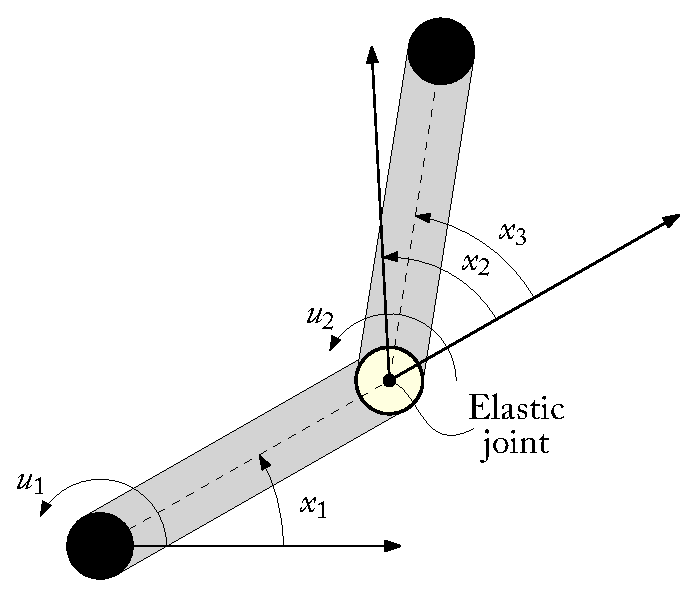
\includegraphics[width=0.4\linewidth]{figures/chapter_4/robotic_arm.eps}
  \caption{Robot arm control problem.}
  \label{chap5:fig:robotic_arm}
\end{figure}

\begin{table}
  \caption{Expression complexity encountered throughout the index reduction of the robotic arm problem~\cite{brenan1995numerical} \ac{DAE} system. \emph{Legend}: $\cf$ = functions, $\ca$ = additions, $\cm$ = multiplications, and $\cd$ = divisions.}
  \label{chap5:tab:tppc_robot}
  \centering
  \resizebox{\textwidth}{!}{%
  {\footnotesize\begin{tabular}{cccc}
    \multicolumn{4}{c}{\textbf{Robotic Arm~\cite{pryce1998solving}}} \\
    \toprule
    \textbf{Original \acp{DAE}} & \multicolumn{3}{c}{$\mF = 125\cf + 19\cd + 56\cm + 64\ca$ \quad $\mh = 0$} \\
    \midrule
    \textbf{Reduction step} & $\mE$ & $\mg$ & $\ma$ \\
    \midrule
    Index-5 \acp{DAE} & $0$ & $66\cf + 3\cd + 50\cm + 35\ca$ & $16\cf + 12\ca$ \\
    Index-4 \acp{DAE} & $0$ & $66\cf + 3\cd + 50\cm + 35\ca$ & $24\cf + 6\cm + 14\ca$ \\
    Index-3 \acp{DAE} & $0$ & $66\cf + 3\cd + 50\cm + 35\ca$ & $162\cf + 2\cd + 138\cm + 114\ca$ \\
    Index-2 \acp{DAE} & $14\cf + 2\cd + 6\cm + 6\ca$ & $372\cf + 4\cd + 375\cm + 253\ca$ & $972\cf + 1\cd + 1062\cm + 770\ca$ \\
    Index-1 \acp{DAE} & $14\cf + 2\cd + 6\cm + 6\ca$ & $372\cf + 4\cd + 375\cm + 253\ca$ & $\star (6.5\cf + 5.6\cm + 1.8\ca)\cdot10^{6} + 4\cd$ \\
    Index-0 \acp{DAE} & $\star (8.3\cf + 7.1\cm + 2.3\ca)\cdot10^{7} + 58\cd$ & $(2.4\cf + 2.0\cm + 0.9\ca)\cdot10^{6} + 8\cd$ & $0$ \\
    \midrule
    \textbf{Reduced \acp{DAE}} & \multicolumn{3}{c}{$\star \mF = (8.6\cf + 7.3\cm + 2.4\ca)\cdot10^{7} + 66\cd$ \quad $\star \mh = (6.5\cf + 5.6\cm + 1.8\ca)\cdot10^{6} + 7\cd$} \\
    \bottomrule
    \end{tabular}}
    }
\end{table}

\begin{table}
  \caption{Expression complexity encountered throughout the index reduction with the aid of hierarchical representation of the robotic arm problem~\cite{brenan1995numerical} \ac{DAE} system. \emph{Legend}: $\cf$ = functions, $\cv$ = veiling variables, $\ca$ = additions, $\cm$ = multiplications, and $\cd$ = divisions.}
  \label{chap5:tab:tppc_robot_veil}
  \centering
  {\footnotesize\begin{tabular}{cccc}
    \multicolumn{4}{c}{\textbf{Robotic Arm~\cite{pryce1998solving}}} \\
    \toprule
    \textbf{Original \acp{DAE}} & \multicolumn{3}{c}{$\mF = 125\cf + 19\cd + 56\cm + 64\ca$ \quad $\mh = 0$ \quad $\mv = 0$} \\
    \midrule
    \textbf{Reduction step} & $\mE$ & $\mg$ & $\ma$ \\
    \midrule
    Index-5 \acp{DAE} & $0$ & $66\cf + 3\cd + 50\cm + 35\ca$ & $16\cf + 12\ca$ \\
    Index-4 \acp{DAE} & $0$ & $66\cf + 3\cd + 50\cm + 35\ca$ & $24\cf + 6\cm + 14\ca$ \\
    Index-3 \acp{DAE} & $0$ & $66\cf + 3\cd + 50\cm + 35\ca$ & $162\cf + 2\cd + 138\cm + 114\ca$ \\
    Index-2 \acp{DAE} & $14\cf + 2\cd + 6\cm + 6\ca$ & $66\cf + 1\cv + 3\cd + 51\cm + 35\ca$ & $1\cm + 1\cv$ \\
    Index-1 \acp{DAE} & $2\cv + 1\ca$ & $66\cf + 1\cv + 3\cd + 51\cm + 35\ca$ & $9\cf + 4\cv + 2\cd + 8\cm + 5\ca$ \\
    Index-0 \acp{DAE} & $7\cv + 1\cd + 2\cm + 2\ca$ & $66\cf + 2\cv + 3\cd + 52\cm + 35\ca$ & $0$ \\
    \midrule
    \textbf{Reduced \acp{DAE}} & \multicolumn{3}{c}{$\mF = 90\cf + 9\cv + 4\cd + 63\cm + 48\ca$ \quad $\mh = 202\cf + 5\cv + 4\cd + 141\cm + 130\ca$} \\
    \bottomrule
  \end{tabular} \\[0.5em]
  \begin{tabular}{cc}
    \multicolumn{2}{c}{Hierarchical representation details (29 veils)} \\
    \toprule
    \textbf{Original \acp{DAE}} & $\mv = 0$ \\
    \midrule
    \textbf{Reduction step} & $\mv$ \\
    \midrule
    Index-5 \acp{DAE} & $0$ \\
    Index-4 \acp{DAE} & $0$ \\
    Index-3 \acp{DAE} & $0$ \\
    Index-2 \acp{DAE} & $1278\cf + 3\cv + 6\cd + 1319\cm + 918\ca$ \\
    Index-1 \acp{DAE} & $8401\cf + 20\cv + 24\cd + 9451\cm + 6095\ca$ \\
    Index-0 \acp{DAE} & $37010\cf + 558\cv + 56\cd + 45087\cm + 28665\ca$ \\
    \midrule
    \textbf{Reduced \acp{DAE}} & $\mv = 37010\cf + 558\cv + 56\cd + 45087\cm + 28665\ca$ \\
    \bottomrule
  \end{tabular}}
\end{table}

The complexity of expressions encountered throughout the index reduction is detailed in Table~\ref{chap5:tab:tppc_robot}. Notably, the index reduction algorithm effectively reduces the system to index-0 without introducing any veiling variable, however, substantial expression growth is observed. The simplification of the expressions within \SI{100}{\second} of \ac{CPU} time is not feasible. Hierarchical representation through veiling variables is necessary to simplify the handling of the system expressions. The complexity of the expressions encountered throughout the index reduction with the aid of hierarchical representation is detailed in Table~\ref{chap5:tab:tppc_robot_veil}. Here, it can be noticed that the introduction of veiling variables effectively reduces the overall expression complexity by 3 orders of magnitude. This can be attributed to the fact that the chunks of the system are now more efficiently handled by the \ac{CAS}, and simplification can be effectively performed.

The numerical integration of the reduced \ac{DAE} system is performed using both the \Maple{} and \Indigo{} numerical solvers. In this regard, \Maple{} is not able to integrate the original \ac{DAE} system due to the incapacity of projecting the initial values into the solution space. Conversely, the numerical integration of the reduced \ac{DAE} system using the RadauIIA5 \Indigo{} numerical solver is successful in the interval $t \in \RSI{0}{0.98}{\second}$. It must be pointed out that this system presents many singularities that hinder a flawless integration (refer to~\cite{schwarz2020singularities} for a detailed analysis). For what concerns \Mathematica{} and \Matlab{} performances, the tests we performed showed that both solvers are not able to integrate the original \ac{DAE} system due to the incapacity of projecting the initial values into the solution space. Furthermore, the Pantelides algorithm implemented in \Matlab{} is not able to reduce the index of the system to index-1.

\section{Electrical Circuits}
\label{chap5:sec:electrical_circuits}

Historically, the \acp{DAE} of electrical networks stimulated the study of \acp{DAE} and their solutions since the early 70s~\cite{gear1971simultaneous}. \acp{DAE} encountered in this domain exhibit a distinct structure, somewhat different from those arising from mechanical systems or \ac{TPPC} problems. Typically, these \acp{DAE} are large and sparse, often linear, although non-linearities may arise from certain circuit components. Our focus here is not to give a detailed account of circuit design, but rather to illustrate the types of \acp{DAE} that may arise and how various aspects of the circuit influence \ac{DAE} system properties such as index, solvability, and numerical solution.

Consider an electrical network comprising $b$ branches connected to $n$ nodes. Assigning a current variable $i_b$ to each branch and a voltage variable $v_n$ to each node, the circuit equations stem from Kirchoff's laws, \ie{} the algebraic sum of currents into a node is zero, and the algebraic sum of the voltage drops around a loop is zero. By convention, current denotes the net flow of positive charge, with a designated current direction along each branch assigned by designating one node as negative and the other as positive (with current flowing from positive to negative). The circuit's topology can be described by a $b \times n$ network incidence matrix $\m{A}$. The $(i,j)$ element of $\m{A}$ is $\pm1$ if node $j$ is the $\pm$ node for the $i$-th branch. Denoting $\m{i}_b$ as the vector of current variables, Kirchoff's current law simply states that $\m{A}^\top\m{i}_b = 0$. The voltage drop across each branch is defined as the difference between the voltage at the positive node and that at the negative node. These branch voltages $\m{v}_b$ can be expressed in terms of the nodal voltages $\m{v}_n$ as $\m{v}_b = \m{A}\m{v}_n$.

Linear circuits composed of resistors, capacitors, and inductors can result in large sparse linear \acp{DAE}. In these circuits, the voltage-current relationship across a resistor branch follows Ohm's law, $v_r = Ri_r$, with a positive resistance $R$. Similarly, the voltage-current characteristics of linear capacitors and inductors satisfy $i_c = C\de{}v_c/\de{}t$ and $v_l = L\de{}i_l/\de{}t$, respectively. However, the inclusion of transistors or unicursal elements tends to introduce non-linearity into \ac{DAE} systems. The solvability of \acp{DAE} arising from linear circuits lacking operational amplifiers is solely influenced by the network topology. However, circuits containing differential amplifiers, typically realized using operational amplifiers, may give rise to \acp{DAE} of arbitrarily high index. \acp{DAE} arising from linear circuits incorporating operational amplifiers depends on the specific voltage-current characteristics of the circuit components for solvability. Moreover, the number of independent \acp{IC} may vary depending on specific circuit parameter values. The potential for arbitrarily high-index \acp{DAE} originating from circuits is demonstrated in examples such as a cascade of differential amplifiers. Furthermore, high-index \acp{DAE} may emerge when different variables are designated as inputs and outputs. For example, whether a device functions as a differentiator or an integrator depends on the designation of inputs and outputs~\cite{brenan1995numerical}.

In the following, we present three examples of electrical circuits, the first being an eight-node transistor amplifier, the second an electric ring modulator, and the third a cascade of differential amplifiers. The first two examples are taken from~\cite{lioen1998test, mazzia2008test}, while the third is taken from~\cite{brenan1995numerical}.

\subsection{Eight-Node Transistor-Amplifier}

This problem originates from electrical circuit analysis, and it is a model for the transistor amplifier. The diagram of the circuit is given in Figure~\ref{chap5:fig:transistor_amplifier}. Here $U_e$ is the input signal and the amplified output signal can be found in point 8. The circuit is described by a system of \acp{DAE} of index-1, consisting of 8 equations, which ca be written in matrix form as $\m{M}\m{x}^\prime = \m{f}(\m{x},t)$, where $\m{x} = [x_1, \dots, x_8]^\top$, $\m{M}$ and $\m{f}(\m{x},t)$ given by
%
\begin{equation}
  \m{M} = \begin{bmatrix}
    -C_1 & C_1 & 0 & 0 & 0 & 0 & 0 & 0 \\
    C_1 & -C_1 & 0 & 0 & 0 & 0 & 0 & 0 \\
    0 & 0 & -C_2 & 0 & 0 & 0 & 0 & 0 \\
    0 & 0 & 0 & -C_3 & C_3 & 0 & 0 & 0 \\
    0 & 0 & 0 & C_3 & -C_3 & 0 & 0 & 0 \\
    0 & 0 & 0 & 0 & 0 & -C_4 & 0 & 0 \\
    0 & 0 & 0 & 0 & 0 & 0 & -C_5 & C_5 \\
    0 & 0 & 0 & 0 & 0 & 0 & C_5 & -C_5
  \end{bmatrix} \, \text{,}
\end{equation}
%
\begin{equation}
  \m{f}(\m{x},t) = \begin{bmatrix}
    -\dfrac{U_e(t)}{R_0} + \dfrac{x_1}{R_0} \\
    -\dfrac{U_b}{R_2} + x_2\left(\dfrac{1}{R_1}+\dfrac{1}{R_2}\right) - (\alpha-1)g(x_2-x_3) \\
    -g(x_2-x_3)+\dfrac{x_3}{R_3} \\
    -\dfrac{U_b}{R_4} + \dfrac{x_4}{R_4} + \alpha g(x_2-x_3) \\
    -\dfrac{U_b}{R_6} + x_5\left(\dfrac{1}{R_5} + \dfrac{1}{R_6}\right)-(\alpha-1) g(x_5-x_6) \\
    -g(x_5-x_6) + \dfrac{x_6}{R_7} \\
    -\dfrac{U_b}{R_8} + \dfrac{x_7}{R_8} + \alpha g(x_5-x_6) \\
    \dfrac{x_8}{R_9}
  \end{bmatrix} \, \text{,}
\end{equation}
%
where $g(x) = \beta(\exp(x/U_f) - 1)\,\USI{\ampere}$, and $U_e(t) = 0.1\sin(200 \pi t)\,\USI{\volt}$. \acp{IC} at $t = 0$ and parameters are given by
%
\begin{equation*}
  \m{x}_0 = \begin{bmatrix}
    0 \\
    U_b/(R_2/R_1 + 1) \\
    U_b/(R_2/R_1 + 1) \\
    U_b \\
    U_b/(R_6/R_5 + 1) \\
    U_b/(R_6/R_5 + 1) \\
    U_b \\
    0 \\
  \end{bmatrix} \, \text{,}
  \qquad \text{and} \qquad
  \begin{array}{l}
    U_b = \SI{6}{\volt} \, \text{,} \\
    U_f = \SI{0.026}{\volt} \, \text{,} \\
    \alpha = 0.99 \, \text{,} \\
    \beta = \SI{10^-6}{\ampere} \, \text{,} \\
    R_0 = \SI{1}{\kilo\ohm} \, \text{,} \\
    R_k = \SI{9}{\kilo\ohm} ~ \text{with} ~ k=1, \dots, 9 \, \text{,} \\
    C_k = \SI{k}{\micro\farad} ~ \text{with} ~ k=1, \dots, 9 \, \text{.} \\
  \end{array} \, \text{.}
\end{equation*}

\begin{figure}
  \centering
  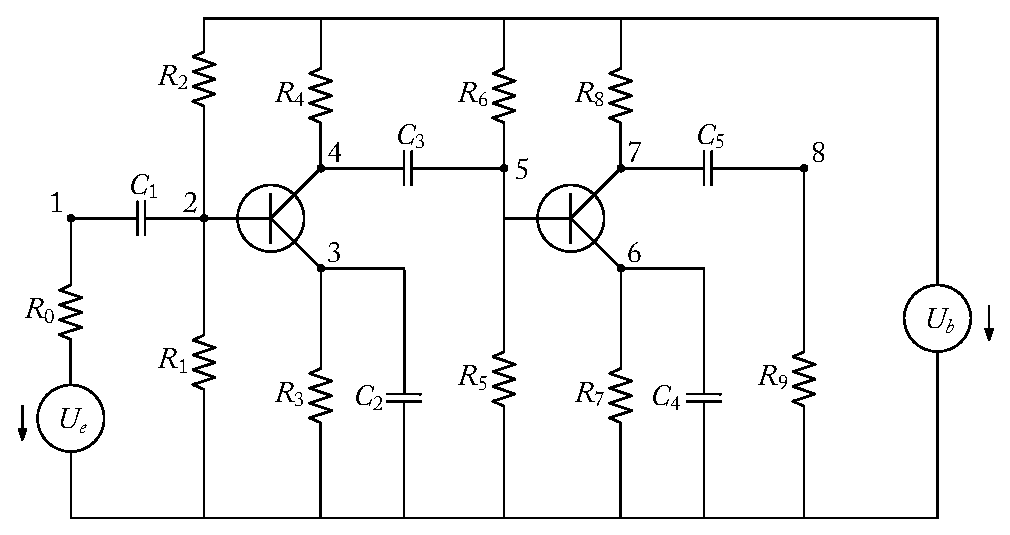
\includegraphics[width=0.7\textwidth]{figures/chapter_4/transistor_amplifier.eps}
  \caption{Eight-node transistor-amplifier circuit~\cite{lioen1998test, mazzia2008test}.}
  \label{chap5:fig:transistor_amplifier}
\end{figure}

The index reduction process is smoothly performed, and the complexity of the expressions encountered throughout the index reduction is detailed in Table~\ref{chap5:tab:tppc_robot}. As we can see, the expression complexity is not affected by the index reduction process. The numerical integration of the reduced \ac{DAE} system is performed using both the \Maple{} and \Indigo{} numerical solvers. In this regard, \Maple{}, \Mathematica{}, \Matlab{} (both Pantelides and Gaussian elimination), and \Indigo{} can integrate the original \ac{DAE} system in the specified time interval $t \in \RSI{0}{0.2}{\second}$.

\begin{figure}[htb]
  \centering
  \small{\includetikz{figures/chapter_4/transistor_amplifier.tex}}
  \caption{Transistor amplifier circuit integration results~\cite{lioen1998test, mazzia2008test} in the time interval $t \in \RSI{0}{0.2}{\second}$. Notice that the output signal $U_8$ is equal to the state variable $x_8$. \emph{Legend}: \textcolor{mycolor1}{$\blacksquare$} input signal $U_e(t)$, and \textcolor{mycolor2}{$\blacksquare$} output signal $U_8$.}
  \label{chap5:fig:transistor_amplifier_results}
\end{figure}

\begin{table}
  \caption{Expression complexity encountered throughout the index reduction of the eight-node transistor-amplifier problem~\cite{lioen1998test, mazzia2008test} \ac{DAE} system. \emph{Legend}: $\cf$ = functions, $\ca$ = additions, $\cm$ = multiplications, and $\cd$ = divisions.}
  \label{chap5:tab:tppc_robot}
  \centering
  {\footnotesize\begin{tabular}{cccc}
    \multicolumn{4}{c}{\textbf{Eight-Nodes Transistor-Amplifier~\cite{lioen1998test, mazzia2008test}}} \\
    \toprule
    \textbf{Original \acp{DAE}} & \multicolumn{3}{c}{$\mF = 55\cf + 21\cd + 29\cm + 41\ca$ \quad $\mh = 0$} \\
    \midrule
    \textbf{Reduction step} & $\mE$ & $\mg$ & $\ma$ \\
    \midrule
    Index-1 \acp{DAE} & $5\ca$ & $17\cf + 11\cd + 22\cm + 20\ca$ & $19\cf + 12\cd + 44\cm + 24\ca$ \\
    Index-0 \acp{DAE} & $24\cf + 26\cd + 24\cm + 24\ca$ & $18\cf + 12\cd + 26\cm + 20\ca$ & $0$ \\
    \midrule
    \textbf{Reduced \acp{DAE}} & \multicolumn{3}{c}{$\mF = 74\cf + 26\cd + 87\cm + 49\ca$ \quad $\mh = 19\cf + 12\cd + 44\cm + 26\ca$} \\
    \bottomrule
    \end{tabular}}
\end{table}

\subsection{Electric Ring Modulator}

The electric ring modulator is an interesting example of a system whose structure depends on the specific values of the parameters. The system is in the form $\m{M}\m{x}^\prime = \m{f}(\m{x},t)$, where $\m{x} = [x_1, \dots, x_{15}]^\top$, $\m{M}$ and $\m{f}(\m{x},t)$ being given by
%
\begin{equation}
  \m{M} = \mathrm{diag}(C, C, C_s, C_s, C_s, C_s, C_p, L_h, L_h, L_{s2}, L_{s3}, L_{s2}, L_{s3}, L_{s1}, L_{s1}) \, \text{,}
\end{equation}
%
\begin{equation}
  \m{f}(\m{x},t) = \begin{bmatrix}
    x_8 - (x_{10} + x_{11})/2 + x_{14} - x_1/R \\
    x_9 - (x_{12} + x_{13})/2 + x_{15} - x_2/R \\
    x_{10} - q(U_{d1}) + q(U_{d4}) \\
    -x_{11} + q(U_{d2}) - q(U_{d3}) \\
    x_{12} + q(U_{d1}) - q(U_{d3}) \\
    -x_{13} - q(U_{d2}) + q(U_{d4}) \\
    -x_7/R_p + q(U_{d1}) + q(U_{d2}) - q(U_{d3}) - q(U_{d4}) \\
    x_1 \\
    x_2 \\
    x_1/2 - x_3 - R_{g2}x_{10} \\
    -x_1/2 + x_4 - R_{g3}x_{11} \\
    x_2/2 - x_5 - R_{g2}x_{12} \\
    -x_2/2 + x_6 - R_{g3}x_{13} \\
    -x_1 + U_{in1}(t) - (R_i + R_{g1})x_{14} \\
    -x_2 - (R_c+R_{g1})x_{15}
  \end{bmatrix} \, \text{,}
\end{equation}
%
where
%
\begin{equation*}
  \begin{array}{l}
    U_{d1} = x_3 - x_5 - x_7 - U_{in2}(t) \, \text{,} \\
    U_{d2} = -x_4 + x_6 - x_7 - U_{in2}(t) \, \text{,} \\
    U_{d3} = x_4 + x_5 + x_7 + U_{in2}(t) \, \text{,} \\
    U_{d4} = -x_3 - x_6 + x_7 + U_{in2}(t) \, \text{,} \\
    q(U) = \gamma(exp(\delta U) - 1) \, \text{,} \\
    U_{in1}(t) = 1/2 \sin(2000 \pi t) \, \text{,} \\
    U_{in2}(t) = 2 \sin(20000 \pi t) \, \text{.}
  \end{array}
\end{equation*}
%
\acp{IC} at $t = 0$ and parameters are given by $\m{x}_0 = [0, 0, 0, 0, 0, 0, 0, 0, 0, 0, 0, 0, 0, 0, 0]^\top$, and
%
\begin{equation*}
  \begin{array}{l}
    C = \SI{16}{\nano\farad} \, \text{,} \\
    C_s = 0~\text{or}~\SI{2}{\pico\farad} \, \text{,} \\
    C_p = \SI{100}{\nano\farad} \, \text{,} \\
    L_h = \SI{4.45}{\henry} \, \text{,} \\
    L_{s1} = \SI{2}{\milli\henry} \, \text{,} \\
    L_{s2} = \SI{0.5}{\milli\henry} \, \text{,} \\
    L_{s3} = \SI{0.5}{\milli\henry} \, \text{,} \\
    \gamma = 40.67286402 \, \text{,} \\
  \end{array}
  \qquad
  \begin{array}{l}
    R = \SI{25}{\kilo\ohm} \, \text{,} \\
    R_p = \SI{50}{\ohm} \, \text{,} \\
    R_{g1} = \SI{36.3}{\ohm} \, \text{,} \\
    R_{g2} = \SI{17.3}{\ohm} \, \text{,} \\
    R_{g3} = \SI{17.3}{\ohm} \, \text{,} \\
    R_{i} = \SI{50}{\ohm} \, \text{,} \\
    R_{c} = \SI{600}{\ohm} \, \text{,} \\
    \delta = 17,7493332 \, \text{.} \\
  \end{array} \, \text{.}
\end{equation*}
%
It must be pointed out that if $C_s \neq 0$, the system is an \acp{ODE}, otherwise, it is an index-2 \ac{DAE} system. In the original test problem in~\cite{lioen1998test, mazzia2008test}, the authors set $C_s = \SI{2}{\pico\farad}$ to obtain an \ac{ODE} system. In Figure~\ref{chap5:fig:ring_modulator}, the electric ring modulator circuit is shown.

Considering $C_s = 0$, the index reduction process is flawlessly performed through the presented algorithm, complexity of the expressions encountered throughout the index reduction is detailed in Table~\ref{chap5:tab:tppc_robot}. Numerical integration in the specified time interval $t \in \RSI{0}{1}{\milli\second}$ is successfully performed by \Indigo{} numerical solvers. Conversely, \Maple{} is not able to integrate the original \ac{DAE} due to computational time exceeding \SI{100}{\second}. Results of the numerical integration are shown in Figure~\ref{chap5:fig:ring_modulator_results}, where the modulated output signal $U_2$ is represented. Notice that the modulated output signal is strongly influenced by the $C_s = 0$ assumption.

\begin{figure}
  \centering
  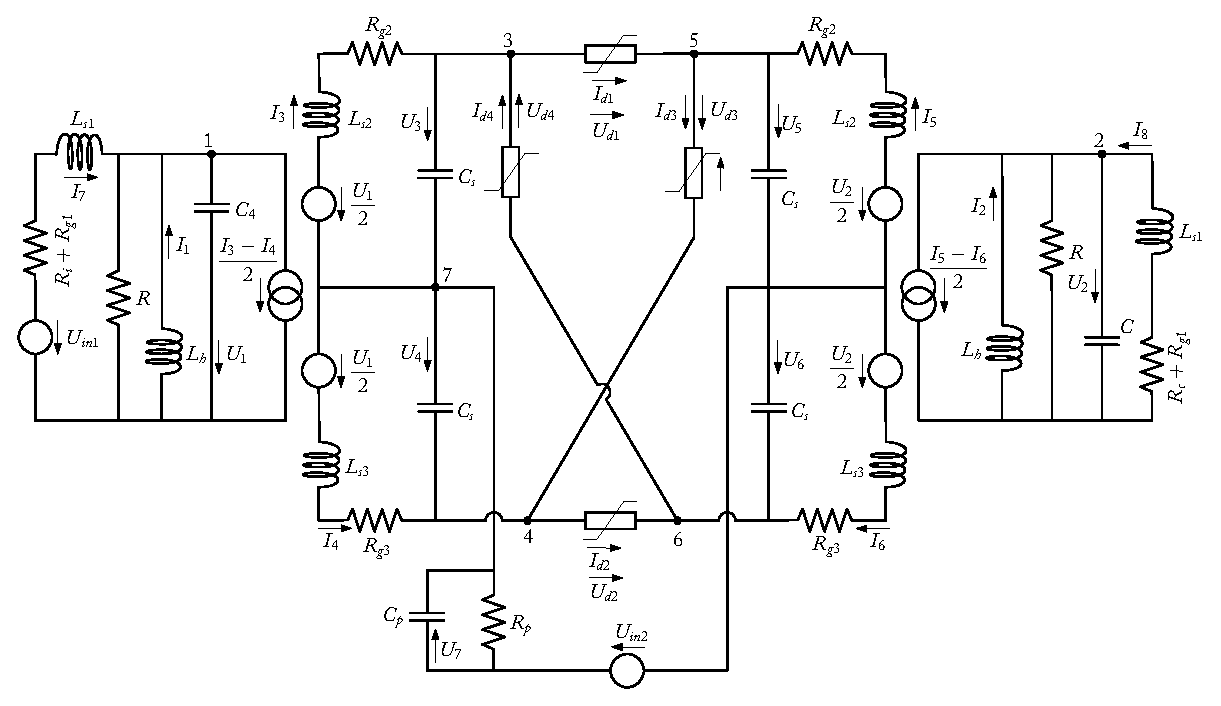
\includegraphics[width=1.0\textwidth]{figures/chapter_4/ring_modulator.eps}
  \caption{Electric ring modulator circuit~\cite{lioen1998test, mazzia2008test}.}
  \label{chap5:fig:ring_modulator}
\end{figure}

\begin{table}
  \caption{Expression complexity encountered throughout the index reduction of the electric ring modulator problem~\cite{lioen1998test, mazzia2008test} \ac{DAE} system. \emph{Legend}: $\cf$ = functions, $\ca$ = additions, $\cm$ = multiplications, and $\cd$ = divisions.}
  \label{chap5:tab:tppc_robot}
  \centering
  {\footnotesize\begin{tabular}{cccc}
    \multicolumn{4}{c}{\textbf{Electric Ring Modulator~\cite{lioen1998test, mazzia2008test}}} \\
    \toprule
    \textbf{Original \acp{DAE}} & \multicolumn{3}{c}{$\mF = 116\cf + 3\cd + 75\cm + 92\ca$ \quad $\mh = 0$} \\
    \midrule
    \textbf{Reduction step} & $\mE$ & $\mg$ & $\ma$ \\
    \midrule
    Index-2 \acp{DAE} & $0$ & $51\cf + 3\cd + 41\cm + 41\ca$ & $44\cf + 32\cm + 36\ca$ \\
    Index-1 \acp{DAE} & $86\cf + 68\cm + 66\ca$ & $262\cf + 13\cd + 416\cm + 220\ca$ & $10\cf + 2\cd + 18\cm + 11\ca$ \\
    Index-0 \acp{DAE} & $86\cf + 12\cd + 72\cm + 70\ca$ & $262\cf + 13\cd + 416\cm + 220\ca$ & $0$ \\
    \midrule
    \textbf{Reduced \acp{DAE}} & \multicolumn{3}{c}{$\mF = 335\cf + 15\cd + 537\cm + 256\ca$ \quad $\mh = 54\cf + 2\cd + 50\cm + 47\ca$} \\
    \bottomrule
    \end{tabular}}
\end{table}

\begin{figure}[htb]
  \centering
  \small{\includetikz{figures/chapter_4/ring_modulator.tex}}
  \caption{Electric ring modulator circuit integration results~\cite{lioen1998test, mazzia2008test} in the time interval $t \in \RSI{0}{1}{\milli\second}$. The lines represent the modulated output signal $U_2$, which is equal to the state variable $x_2$. \emph{Legend}: \textcolor{mycolor1}{$\blacksquare$} output signal $U_2$ with $C_s = \SSI{0}{\pico\farad}$ (\ac{DAE} system), \textcolor{mycolor2}{$\blacksquare$} output signal $U_2$ with $C_s = \SSI{2}{\pico\farad}$ (\ac{ODE} system).}
  \label{chap5:fig:ring_modulator_results}
\end{figure}

\subsection{Cascade of Differential Amplifiers}

The cascade of differential amplifiers is an example of a system whose index can be arbitrarily high, depending on how many operational amplifiers are cascaded. If we consider a circuit with one differential amplifier as shown in Figure~\ref{chap:4:fig:diffamp_single} and, assuming that the operational amplifier is ideal, the circuit equations lead to the relation $x(t) = -C R U(t)^{\prime}$ where $U(t)$ is the generator voltage. Since the solution to the circuit equations involves at least one derivative of the input function, the system must be index-1. By cascading a series of $p \in \mathcal{N}$ differential amplifiers in a circuit as in Figure~\ref{chap:4:fig:diffamp_cascade}, we can see that the resulting \acp{DAE} index is equal to $p$. Specifically, the voltage at the output of the $p$-th differential amplifier is given by $x_p(t) = -C_p R_p x_{p-1}(t)^{\prime}$, where $v(t) = -C_1 R_1 U(t)^{\prime}$. Thence the following system of equations is obtained
%
\begin{equation*}
  \begin{cases}
    x_1(t) = -C_1 R_1 U(t)^{\prime} \\
    x_2(t) = -C_2 R_2 x_1(t)^{\prime} \\
    ~\vdots \\
    x_p(t) = -C_p R_p x_{p-1}(t)^{\prime}
  \end{cases}
  %
  \quad \text{whose analytical solution is} \quad
  %
  x_i(t) = \prod_{j=1}^{i} (-C_j R_j) \dfrac{\de{}^{i}}{\de{}t^{i}}U(t) \, \text{.}
\end{equation*}
%
Consistent \acp{IC} at $t = t_0$ can be easily obtained by evaluating the analytical solution at $t = t_0$, \ie{},
%
\begin{equation*}
  \m{x}_0 = \begin{bmatrix}
    -C_1 R_1 \left.\dfrac{\de{}}{\de{}t}U(t)\right|_{t=t_0} \\
    \vdots \\
    \displaystyle\prod_{j=1}^{p} (-C_j R_j) \left.\dfrac{\de{}^{p}}{\de{}t^{p}}U(t)\right|_{t=t_0}
  \end{bmatrix} \, \text{.}
\end{equation*}

\begin{figure}[htb]
  \centering
  \begin{subfigure}[t]{0.26\textwidth}
    \centering
    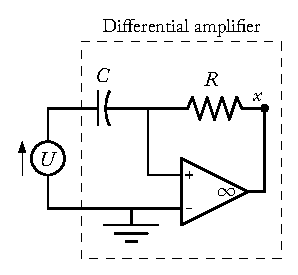
\includegraphics[width=1.0\textwidth]{figures/chapter_4/differential_amplifier_single.eps}
    \caption{Circuit with a single differential amplifier.}
    \label{chap:4:fig:diffamp_single}
  \end{subfigure}%
  \hfill%
  \begin{subfigure}[t]{0.72\textwidth}
    \centering
    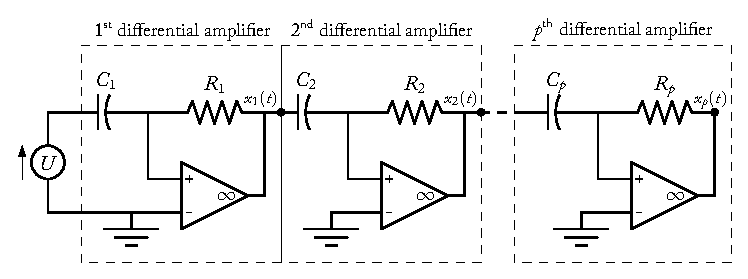
\includegraphics[width=1.0\textwidth]{figures/chapter_4/differential_amplifier_cascade.eps}
    \caption{Circuit with a cascade of $p$ differential amplifiers.}
    \label{chap:4:fig:diffamp_cascade}
  \end{subfigure}
  \caption{Circuit diagrams for the cascade of differential amplifiers problem~\cite{brenan1995numerical}.}
  \label{chap:4:fig:diffamp_all}
\end{figure}

The index reduction of such a system, which falls under the category of linear \acp{DAE}, is pretty much straightforward. \Indigo{} can reduce to index-0 systems made of up to $p = 100$ differential amplifiers, even if the performance of the reduction process is strongly linked to the capabilities of \Maple{} symbolic kernel to deal with sparse large matrices. An interesting aspect that this last application brings to light is how systematically the index reduction process is performed through \Indigo{}. The system is transformed in the form $\mE \, \mxp = \mg$ with $\ma = \m{0}$, which is explicitly given by
%
\begin{equation*}
  \left[\begin{array}{ccc|c}
    -C_2 R_2 & & & 0 \\
    & \ddots & & \vdots \\
    & & -C_p R_p & 0 \\
  \end{array}\right]
  %
  \left[\begin{array}{c}
    x_1^{\prime} \\ \vdots \\ x_{p-1}^{\prime} \\ \hline x_p^{\prime}
  \end{array}\right] = \left[\begin{array}{c}
    x_2 \\ \vdots \\ x_p
  \end{array}\right]
  %
  \quad \text{with} \quad
  %
  \ma = \begin{bmatrix}
    - x_1 - C_1 R_1 \dfrac{\de{}}{\de{}t}U(t)
  \end{bmatrix} \, \text{.}
\end{equation*}
%
Then the index reduction is performed $p$ times, and the system $\mE \, \mxp = \mg$ at the $k$-th index reduction step is equal to
%
\begin{equation*}
  \left[\begin{array}{ccc|c|ccc}
    1 &        &   & \\
      & \ddots &   & \\
      &        & 1 & \\ \hline
      &        &   & & -C_{k+2} R_{k+2} \\
      &        &   & & & \ddots \\
      &        &   & & & & -C_{p} R_{p} \\ \hline
      &        &   & 1 \\
  \end{array}\right]
  %
  \left[\begin{array}{c}
    x_1^{\prime} \\ \vdots \\ x_{k+1}^{\prime} \\ \hline
    x_{k+2}^{\prime} \\ \vdots \\ x_{p-1}^{\prime} \\ \hline
    x_p^{\prime}
  \end{array}\right] = \left[\begin{array}{c}
    -C_1R_1 \dfrac{\de{}^2}{\de{}t^2}U(t) \\
    \vdots \\
    \displaystyle\prod_{j=1}^{k-1} (-C_j R_j) \dfrac{\de{}^k}{\de{}t^k}U(t) \\ \hline
    x_{k+2} \\ \vdots \\ x_p \\ \hline
    \displaystyle\prod_{j=1}^{k} (-C_j R_j) \dfrac{\de{}^{k+1}}{\de{}t^{k+1}}U(t)
  \end{array}\right] \, \text{,}
\end{equation*}
%
with algebraic equations $\ma = \m{0}$ and hidden constraints $\mh = \m{0}$ given by
%
\begin{equation*}
  \ma = \begin{bmatrix}
    -x_{k+1} + \displaystyle\prod_{j=1}^{k+1} (-C_j R_j) \dfrac{\de{}^{k+1}}{\de{}t^{k+1}}U(t)
  \end{bmatrix}
  %
  \quad \text{and} \quad
  %
  \mh = \begin{bmatrix}
    -x_{1} - C_1R_1 \dfrac{\de{}}{\de{}t}U(t) \\
    \vdots \\
    -x_k + \displaystyle\prod_{j=1}^{k} (-C_j R_j) \dfrac{\de{}^{k}}{\de{}t^{k}}U(t)
  \end{bmatrix} \, \text{.}
\end{equation*}
%
Finally, at the $p$\textsuperscript{th} step, the reduced index-0 system is written as
%
\begin{equation*}
  \begin{bmatrix}
    1 & & \\
    & \ddots & \\
    & & 1 \\
  \end{bmatrix}
  %
  \begin{bmatrix}
    x_1^{\prime} \\ \vdots \\ x_p^{\prime}
  \end{bmatrix} = \left[\begin{array}{c}
    -C_1R_1 \dfrac{\de{}^{2}}{\de{}t^{2}}U(t) \\
    \vdots \\
    \displaystyle\prod_{j=1}^{p-1} (-C_j R_j) \dfrac{\de{}^{p}}{\de{}t^{p}}U(t)
  \end{array}\right]
  %
  \quad \text{with} \quad
  %
  \mh = \begin{bmatrix}
    -x_{1} - C_1R_1 \dfrac{\de{}}{\de{}t}U(t) \\
    \vdots \\
    -x_k + \displaystyle\prod_{j=1}^{p} (-C_j R_j) \dfrac{\de{}^{p}}{\de{}t^{p}}U(t)
  \end{bmatrix} \, \text{.}
\end{equation*}
%

% % % % % % % % % % % % % % % % % % % % % % % % % % % % % % % % % % % % % % % %

\section{Summary of Results and Discussion}

It is now time to summarize the results obtained from the experiments and discuss the performance of the presented algorithm. To do so we will consider the following aspects: the symbolic index reduction, the numerical integration, and the overall performance of the algorithm throughout the reduction steps. The results are summarized in Table~\ref{chap5:tab:numerical_integration}, where for each example the solution process is summarized in brief. It is important to highlight that in the same table, the examples are numbered according to the order in which they were presented in this chapter, which will be useful for the discussion that follows.

\subsection{Symbolic Index Reduction}

The first aspect to consider is the symbolic index reduction process. Specifically, the presented algorithm can successfully reduce the index of all the example \ac{DAE} systems here considered. The computational cost of the expressions generated during the index reduction procedure is typically comparable to the original \ac{DAE} system in most of the tests. Additionally, we have seen that the specific type of matrix factorization plays a crucial role in the computational cost of the expressions generated during the index reduction process. In this regard, the ``standard'' \ac{LU} factorization is found to produce better results in terms of computational cost than the \ac{FFLU} factorization. Nonetheless, in examples 3, 6, 7 and 11 the expressions generated during the index reduction procedure are significantly more complex than the original \ac{DAE} system. In these cases, the \Maple{} symbolic computation kernel is not able to perform the simplification within \SI{100}{\second} of \ac{CPU} time and the raw expressions are kept in the following reduction steps. As a consequence, the computational cost inherently increases throughout the following reduction steps. Notably, the \ac{DAE} systems that are hard to simplify are those having a matrix $\mA$ that is strongly dependent on the state variables $\mx$ or equivalently that retains complicated divisions in the vector $\mb$. In these cases, the computational cost of the vector $\ma$ increases significantly due to successive and repeated differentiation and symbolic factorization. In examples 3 and 11, the hierarchical pivoting strategy is thereby used to mitigate the expression swell and ensure the successful index reduction of the \ac{DAE} system. In such examples the veiling strategy proved to be of substantial help, effectively reducing the expression complexities and ensuring the successful index reduction of the \ac{DAE} system. On the other hand, in examples 6 and 7, the hierarchical representation is not used on purpose to understand the impact of the expression swell on the numerical integration process.

For the sake of completeness, also the index reduction algorithms provided by \Matlab{} and \Mathematica{} are tested. The results show that both software tools are able to reduce the index of the \ac{DAE} systems, however, the computational cost of the expressions generated during the index reduction procedure cannot be evaluated due to either the lack of a built-in function to compute the expression complexity or the inability to access the reduced \ac{DAE} systems' expressions.

Another aspect that is important to mention is the sudden increase in computational complexity of the expressions generated in the last reduction steps. Even if such a sudden increase is not critical to the correct index reduction as the presented algorithm is insensitive to expression swell, it does undermine the numerical solution efficiency of the final \ac{DAE} system. This highlights the need for further research on expression swell mitigation techniques in symbolic computation (see Section~\ref{chap3:sec:lem}), as well as the need to use integrators that can handle index-1 \acp{DAE}. Specifically, the detection of linear index-1 variables during the index reduction process is would be beneficial to the minimization of the final \ac{DAE} system complexity. This is particularly important for the numerical integration process, as the more complex the expressions, the more computationally expensive the numerical integration process becomes. Discussion on future work (Section~\ref{chap6:sec:future_work}) will provide insights on new developments in this direction.

\subsection{Numerical Integration}

The numerical integration has also been carried out, with outcomes detailed in Table~\ref{chap5:tab:numerical_integration}. This table reports the performance comparison between the joint index reduction algorithm and numerical integration schemes offered by \Maple{} and those of \Indigo{}. To ensure a fair comparison, both \Maple{} and \Indigo{} utilized the \ac{RKF} 4(5) method for numerical integration of the \ac{DAE} system. Identical error tolerances are applied, with a relative tolerance of $10^{-6}$ and an absolute tolerance of $10^{-7}$. The results illustrate that \Indigo{}'s index reduction algorithm implementation effectively generates numerically stable reduced-index \acp{DAE}, ensuring consistent integration across examples. However, exceptions arise in examples 3, 5, 6, 7, 9, 10, 11, 13, and 14. Specifically, in examples 3, 5, 6, 7, 9, 11, and 13, \Maple{} fails to generate code for the reduced-index system within the expected time frame, thus the integration is not performed. This is due to the complexity of the expressions generated during the index reduction procedure, which overloads the \Maple{}'s \texttt{CodeGeneration} package. On the other hand in examples 10 and 14, the numerical integration can not be performed due to the inability of \Maple{} to verify the consistency of the \ac{IVP}. The \Indigo{} numerical integration is successful in all examples, except for example 11, where it fails to generate the code for the reduced-index system within the expected time frame. This is due to the complexity of the expressions generated during the index reduction procedure, which overloads the \Indigo{}'s \texttt{CodeGeneration} package. Notably, in examples 5, 6 and 7 the integration of the reduced-index system is successfully performed using the non-default implicit RadauIIA5 method. Nonetheless, the high expression swell in these examples leads to a significant increase in the computational cost of the numerical integration, however, the numerical stability is not compromised.

\Mathematica{} and \Matlab{} are also tested for numerical integration. The results show that both software tools are able to integrate the original \ac{DAE} systems in the specified time interval. The only exception is example 11, where both fail to integrate the \ac{DAE} system due to the inability to project the \acp{IC} onto the solution manifold.

It is important to highlight that during the numerical integration, the symbolic code is not regenerated, even if the \ac{DAE} system may locally change its index. Indeed, for some numerical values of states and parameters, the \acp{DAE} system structure may change, leading to numerical instability. While this does pose a potential issue, we have not encountered instability in the integration process. The pivot values were continuously monitored during the numerical integration process to ensure that the \ac{DAE} system structure remains consistent, thereby experimentally proving that the presented pivoting strategy is effective.

\setlength\tabcolsep{2.5pt}
\setlength{\LTcapwidth}{\textwidth}
{\footnotesize\centering\begin{longtable}{lccl}
  \caption{Numerical integration results of the reduced-index \ac{DAE} systems. The table reports the name and reference of the \ac{DAE} system, the index of the system, the integration interval $t \in [t_{\text{ini}}, \, t_{\text{end}}]$, and the outcomes of the whole code generation and integration process for both \Maple{} and \Indigo{}. If not otherwise specified, the tests are integrated using an embedded Runge-Kutta-Fehlberg 4(5) method with a relative tolerance of $10^{-6}$ and an absolute tolerance of $10^{-7}$. The computation time limit is \SI{1000}{\second}, to both generate the necessary code and perform numerical computations. \emph{Legend:} \mycheckmark{} successful code generation and numerical integration, \mycrossmark{} errors in the code generation, numerical integration or time expired, and \mywarnmark{} warnings encountered or non-default settings used in the code generation or numerical integration.}
  \label{chap5:tab:numerical_integration}
  \endfirsthead
  \endhead
  %
  \toprule
  \textbf{Integrated \ac{DAE} system} &
  \multicolumn{3}{l}{\textbf{Integration outcomes and errors}} \\
  \midrule
  \multirow{1}{*}{\textbf{1.~~Particle Motion~\cite{campbell1995constraint}}}
    & \Maple{}       & \mycheckmark{}\phantom{\mywarnmark{}} & Success \\ \cmidrule{2-4}
    \multirow{4}{*}{Index-3 \quad $t \in [0, 400\pi]$ seconds} & \Mathematica{} & \mycheckmark{}\phantom{\mywarnmark{}} & Success \\ \cmidrule{2-4}
    & \multirow{2}{*}{\Matlab{}} & \mycheckmark{}\phantom{\mywarnmark{}} & \texttt{reduceDAEIndex} -- Success \\ \cmidrule{3-4}
    &                            & \mycheckmark{}\phantom{\mywarnmark{}} & \texttt{reduceDAEToODE} -- Success \\ \cmidrule{2-4}\cmidrule{2-4}
    & \Indigo{} & \mycheckmark{}\phantom{\mywarnmark{}} & Success \\ \midrule
  \multirow{1}{*}{\textbf{2.~~Car-Axis~\cite{lioen1998test, mazzia2008test}}}
    & \Maple{}       & \mycheckmark{}\phantom{\mywarnmark{}} & Success \\ \cmidrule{2-4}
    \multirow{4}{*}{Index-3 \quad $t \in [0, 3]$ seconds} & \Mathematica{} & \mycheckmark{}\phantom{\mywarnmark{}} & Success \\ \cmidrule{2-4}
    & \multirow{2}{*}{\Matlab{}} & \mycheckmark{}\phantom{\mywarnmark{}} & \texttt{reduceDAEIndex} -- Success \\ \cmidrule{3-4}
    &                            & \mycheckmark{}\phantom{\mywarnmark{}} & \texttt{reduceDAEToODE} -- Success \\ \cmidrule{2-4}\cmidrule{2-4}
    & \Indigo{} & \mycheckmark{}\phantom{\mywarnmark{}} & Success \\ \midrule
  \multirow{1}{*}{\textbf{3.~~Flexible Slider-Crank~\cite{lioen1998test, mazzia2008test}}}
    & \Maple{}  & \mycrossmark{}\phantom{\mywarnmark{}} & Error, time expired in \texttt{dsolve} \\ \cmidrule{2-4}
    Index-3 \quad $t \in [0, 0.1]$ seconds & \Indigo{} & \mycheckmark{}\phantom{\mywarnmark{}} & Success \\ \midrule
  \multirow{1}{*}{\textbf{4.~~2-Pendula~\cite{pryce1998solving}}}
    & \Maple{}  & \mycheckmark{}\phantom{\mywarnmark{}} & Success \\ \cmidrule{2-4}
    Index-5 \quad $t \in [0, 60]$ seconds & \Indigo{} & \mycheckmark{}\phantom{\mywarnmark{}} & Success \\ \midrule
  \multirow{1}{*}{\textbf{5.~~3-Pendula~\cite{nedialkov2008solvingIII}}}
    & \Maple{}  & \mycrossmark{}\phantom{\mywarnmark{}} & Error, time expired in \texttt{dsolve} \\ \cmidrule{2-4}
    Index-7 \quad $t \in [0, 60]$ seconds & \Indigo{} & \mycheckmark{}\mywarnmark{} & Success with RadauIIA5 method \\ \midrule
  \multirow{1}{*}{\textbf{6.~~4-Pendula~\cite{nedialkov2008solvingIII}}}
    & \Maple{}  & \mycrossmark{}\phantom{\mywarnmark{}} & Error, time expired in \texttt{dsolve} \\ \cmidrule{2-4}
    Index-9 \quad $t \in [0, 60]$ seconds & \Indigo{} & \mycheckmark{}\mywarnmark{} & Success with RadauIIA5 method \\ \midrule
  \multirow{1}{*}{\textbf{7.~~5-Pendula~\cite{nedialkov2008solvingIII}}}
    & \Maple{}  & \mycrossmark{}\phantom{\mywarnmark{}} & Error, time expired in \texttt{dsolve} \\ \cmidrule{2-4}
    Index-11 \quad $t \in [0, 60]$ seconds & \Indigo{} & \mycheckmark{}\mywarnmark{} & Success with RadauIIA5 method \\ \midrule
  \multirow{1}{*}{\textbf{8.~~Double-Wishbone Suspension}}
    & \Maple{}  & \mycheckmark{}\phantom{\mywarnmark{}} & Success \\ \cmidrule{2-4}
    Index-3 \quad $t \in [0, 60]$ seconds & \Indigo{} & \mycheckmark{}\phantom{\mywarnmark{}} & Success \\ \midrule
  \multirow{1}{*}{\textbf{9.~~Initial Stage Space Shuttle Reentry~\cite{brenan1995numerical}}}
    & \Maple{}  & \mycrossmark{}\phantom{\mywarnmark{}} & Error, time expired in \texttt{dsolve} \\ \cmidrule{2-4}
    Index-3 \quad $t \in [332.8, 419.8]$ seconds & \Indigo{} & \mycheckmark{}\phantom{\mywarnmark{}} & Success \\ \midrule
  \multirow{1}{*}{\textbf{10.~~Final Stage Space Shuttle Reentry~\cite{brenan1995numerical}}}
    & \Maple{}  & \mycrossmark{}\phantom{\mywarnmark{}} & Error, in \texttt{dsolve/numeric/DAE/checkconstraints} \\ \cmidrule{2-4}
    Index-2 \quad $t \in [0, 300]$ seconds & \Indigo{} & \mycheckmark{}\phantom{\mywarnmark{}} & Success \\ \midrule
  \multirow{1}{*}{\textbf{11.~~Robotic Arm~\cite{pryce1998solving}}}
    & \Maple{}       & \mycrossmark{}\phantom{\mywarnmark{}} & Error, time expired in \texttt{dsolve} \\ \cmidrule{2-4}
    \multirow{4}{*}{Index-5 \quad $t \in [0, 2]$ seconds}
    & \Mathematica{} & \mycrossmark{}\phantom{\mywarnmark{}} & Error, time expired in \texttt{NDSolve} \\ \cmidrule{2-4}
    & \multirow{2}{*}{\Matlab{}} & \mycrossmark{}\phantom{\mywarnmark{}} & \texttt{reduceDAEIndex} -- Error, index reduction not completed \\ \cmidrule{3-4}
    &                            & \mycrossmark{}\phantom{\mywarnmark{}} & \texttt{reduceDAEToODE} -- Error, in \texttt{sym/decic} \\ \cmidrule{2-4}
    & \Indigo{} & \mycrossmark{}\phantom{\mywarnmark{}} & Error, time expired in \texttt{CodeGeneration} \\ \midrule
  \multirow{1}{*}{\textbf{12.~~8-Nodes Transistor-Amplifier~\cite{lioen1998test, mazzia2008test}}}
    & \Maple{}       & \mycheckmark{}\mywarnmark{} & Warning, function evaluations limit exceeded \\ \cmidrule{2-4}
    \multirow{4}{*}{Index-1 \quad $t \in [0, 0.2]$ seconds} & \Mathematica{} & \mycheckmark{}\phantom{\mywarnmark{}} & Success \\ \cmidrule{2-4}
    & \multirow{2}{*}{\Matlab{}} & \mycheckmark{}\phantom{\mywarnmark{}} & \texttt{reduceDAEIndex} -- Success \\ \cmidrule{3-4}
    &                            & \mycheckmark{}\phantom{\mywarnmark{}} & \texttt{reduceDAEToODE} -- Success \\ \cmidrule{2-4}\cmidrule{2-4}
    & \Indigo{} & \mycheckmark{}\phantom{\mywarnmark{}} & Success \\ \midrule
  \multirow{1}{*}{\textbf{13.~~Electric Ring Modulator~\cite{lioen1998test, mazzia2008test}}}
    & \Maple{}  & \mycrossmark{}\phantom{\mywarnmark{}} & Error, time expired in \texttt{dsolve} \\ \cmidrule{2-4}
    Index-2 \quad $t \in [0, 1]$ milliseconds & \Indigo{} & \mycheckmark{}\phantom{\mywarnmark{}} & Success \\ \midrule
  \multirow{1}{*}{\textbf{14.~~Cascaded Differential Amplifiers~\cite{brenan1995numerical}}}
    & \Maple{}  & \mycrossmark{}\phantom{\mywarnmark{}} & Error, in \texttt{dsolve/numeric/DAE/checkconstraints} \\ \cmidrule{2-4}
    Arbitrary high index \quad $t \in [0, 10]$ seconds & \Indigo{} & \mycheckmark{}\phantom{\mywarnmark{}} & Success \\
  \bottomrule
  %
\end{longtable}}


%%!TEX root = ../main.tex

\chapter[DAEs Index Reduction and Numerical Solution]{Differential-Algebraic Equations Index Reduction and Numerical Solution}
\label{chap6:daes}

\subsubsection{Copyright Notice}
Part of this chapter has been first published in
%
\begin{center}
  \begin{minipage}{0.9\textwidth}
    \fullcite{stocco2024symbolic}
  \end{minipage}
\end{center}
\begin{center}
  \begin{minipage}{0.9\textwidth}
    \fullcite{stocco2024matrix}
  \end{minipage}
\end{center}
%
by Springer and Elsevier, respectively. Reproduced with permission from Springer and Elsevier.

\begin{center}
  $\ast$~$\ast$~$\ast$
\end{center}

We present an algorithm for the index reduction of first-order differential-algebraic equations. The proposed approach can be applied to generic differential-algebraic equations and exploits neither a priori knowledge nor ad hoc techniques to leverage the specific formulation of the system. The index reduction is performed only by using symbolic manipulation and linear algebra techniques. It is based on the successive separation of the differential and algebraic equations of the system and the subsequent differentiation of the algebraic part. Improved symbolic matrix factorization is used to perform the differential-algebraic equations partitioning, ensure numerical stability, and limit the expression swell of the reduced-index system. The effectiveness of the algorithm is validated through symbolic-numerical examples on a wide range of systems, including physical systems, engineering applications, and ``artificial'' differential-algebraic equations with specific properties. The proposed symbolic index reduction algorithm is implemented in \Maple{} as part of an open-source library.

% % % % % % % % % % % % % % % % % % % % % % % % % % % % % % % % % % % % % % % %

\section{Introduction}
\label{chap6:sec:introduction}

\acp{DAE} are extensively used in dynamic system modeling. The challenge in numerically solving a \ac{DAE} system is assessed through its differentiation index, commonly referred to as ``the'' index~\cite{campbell1995index}. Achieving accurate simulations necessitates converting high-index \acp{DAE} into low-index counterparts, posing a well-recognized challenge~\cite{petzold1982differential}. This process involves transforming a \ac{DAE} system into an equivalent system with a lower index through successive differentiation of the system equations. For this reason, the differentiation index is roughly defined as the number of times algebraic equations are differentiated to obtain an equivalent system of \acp{ODE} with invariants. Index reduction is a crucial step prior to the numerical integration of \acp{DAE}, as integrating high-index systems can be impractical. The primary obstacle lies in the necessity to solve nonlinear systems of equations at each integration step, which can be computationally expensive and, in certain cases, numerically unstable. Specific numerical techniques, introduced in~\cite{petzold1982differential, thomsen1999numerical, baumgarte1972stabilization}, have been developed to address this challenge. However, these methods are not universally effective and may be inapplicable to some high-index \acp{DAE}. Consequently, index reduction becomes an indispensable preliminary stage before numerical integration~\cite{lamour2013differential}.

Given its complicated nature, index reduction has been the subject of extensive research and is often carried out by leveraging the specific formulation of the \ac{DAE} system, like in the multi-body modeling~\cite{zhou2005implicit, zhou2007symbolic, zhou2007symbolicseq, bayo1988modified, wehage1982generalized}. When the specific formulation of the \ac{DAE} system is not known a priori, or the system is not in a specific form, the index reduction process becomes more challenging. Many current simulation software packages for dynamic systems use index-reduction algorithms based on the \ac{SA} of the system, such as the Pantelides algorithm~\cite{pantelides1988consistent} and the dummy derivatives method~\cite{mattsson1993index}, which are subcases of the Pryce's $\Sigma$-method~\cite{pryce1998solving, pryce2001simple, nedialkov2007solvingI, nedialkov2007solvingII, nedialkov2008solvingIII, nedialkov2015algorithm, tan2016symbolic, mckenzie2017structural}. These algorithms are effective in reducing the index of most of the systems, but they can fail either for numerical cancellations~\cite{iwata2019index} or underestimation of the differentiation index~\cite{pantelides1988consistent, unger1995structural}, like in the case of Rei{\ss}ig's \acp{DAE} family~\cite{reissig2000differential}. Symbolic manipulation is proven to be successful in restating a \acp{DAE} on which the $\Sigma$-method fails to a \acp{DAE} on which the \ac{SA} may succeed~\cite{tan2016symbolic}.

Index reduction based on symbolic-numeric aided \ac{SA} has been successful in handling failures of the Pryce's $\Sigma$-method~\cite{tan2016symbolic} as well as in performing symbolically-informed \ac{SA}~\cite{chowdhry2004symbolic}. This latter \ac{SA} approach, which is named $\sigma v$-method, uses symbolic-numeric \ac{LU} factorization for variable substitution and rank determination on linear constant coefficient \acp{DAE}. A valuable attempt to use pure symbolic manipulation in \acp{DAE} index reduction is presented in~\cite{zhou2005implicit, zhou2007symbolic, zhou2007symbolicseq}, where implicit involutive form and \ac{LU} decomposition are successfully used to reduce the index of a simple constrained multi-body system. It is clear that index reduction algorithms based on pure symbolic matrix factorization represent a viable alternative to classic \ac{SA} techniques. However, symbolic matrix factorization feasibility is strongly tied to the performance of the symbolic computation kernel and its capabilities~\cite{zhou2008fraction}. Large expressions can lead to strong performance degradation of the kernel. Techniques aimed at limiting this decrease of performance while performing symbolic linear algebra operations are presented in~\cite{zhou2006hierarchical, zhou2007symbolic, zhou2007symbolicseq}. In these works, the hierarchical representation of expressions is applied to matrix factorization tasks. Nonetheless, the \LULEM{} package~\cite{carette2006linear}, which implements large expression management strategies in \ac{LU} decomposition, significantly outperforms the \Maple{}'s built-in matrix factorization routines.

Following this brief introduction of the most widely recognized index reduction algorithms, we provide an overview of the specific index reduction algorithms found in current state-of-the-art software. The following list is limited to the most prominent solutions dedicated to dynamic system modeling and simulation that are widely adopted in both academia and industry.
%
\begin{itemize}
  \setlength{\itemsep}{-0.2em}
  \item \Matlab{} uses the Pantelides algorithm~\cite{pantelides1988consistent} to reduce the \acp{DAE} to index-1. Alternatively, or if the latter fails, the more reliable but slower Gaussian elimination algorithm can be employed to obtain an index-0 \ac{DAE} system~\cite{matlab}.
  \item \textsc{Modelica}-based software~\cite{mattsson1997modelica, mattsson1998physical} and \textsc{ModelingToolkit}~\cite{modelingtoolkit} employ the Pantelides algorithm~\cite{pantelides1988consistent} along with the dummy derivatives method~\cite{mattsson1993index} to automatically perform the reduction to index-1 \acp{DAE}.
  \item \Mathematica{} offers a comprehensive suite of index reduction algorithms~\cite{mathematica}. It can reduce the index of \acp{DAE} using the Pantelides~\cite{pantelides1988consistent} or structural matrix~ \cite{unger1995structural, chowdhry2004symbolic} methods. Additionally, it implements dummy derivatives~\cite{mattsson1993index} and projection methods for taking hidden constraints into account during numerical integration.
  \item \Maple{} performs symbolic index reduction within the \texttt{dsolve} function~\cite{maple}. However, the implemented algorithms are not documented or referenced. They are likely to be based on the projection method outlined in~\cite{shmoylova2013simplification}. Notably, the patents by the same authors~\cite{postma2012exact, shmoylova2012method, postma2015exact} discuss techniques for eliminating isolated parameters, extracting parameter sub-expressions from \acp{DAE}, and establishing minimal disconnected clusters of parameter sub-expressions. We would like to point out that this information is to be taken with caution, as \Maple{} does not provide specific references on this topic.
\end{itemize}
%
All the showcased software solutions offer integrators for index-0 and index-1 \acp{DAE}. Depending on the system's stiffness, users can select the most appropriate algorithm for numerically integrating the reduced-index system.

The absence of user-invocable standalone functions within the \Maple{} environment that allows for the automatic index reduction of \acp{DAE}, and the inability to extract both the reduced-index system and invariants from the \texttt{dsolve} function, are the primary motivations of this research. Furthermore, recent advances in symbolic matrix factorization, combined with expressions hierarchical representation techniques, provide valuable tools that enable us to further investigate the applicability of a novel algorithm for the index reduction of \ac{DAE} systems, firstly presented in~\cite{stocco2024symbolic} as a preliminary work. The proposed methodology is similar to the previous work of~\citet{chowdhry2004symbolic} and extends it to generic first-order \acp{DAE}, linear in the states' derivatives. Nonetheless, the proposed algorithm does not work on the structural matrix of the system but on the \ac{DAE} system symbolic expressions. Specifically, the idea of using matrix factorization for variable substitution and rank determination is adopted to iteratively separate the differential and algebraic equations of the system. The algebraic equations are then differentiated to obtain an equivalent system with a lower differentiation index. Not less important, new libraries for symbolic matrix factorization (\LAST{}), large expression management (\LEM{}), and signature computation (\SIG{}) are presented. These libraries are based on the \LULEM{} package and extend the work of~\citet{zhou2006hierarchical, carette2006linear} and~\citet{zhou2007symbolic}. The newly presented libraries are designed to ensure the numerical stability of the numerically evaluated expressions, limit the expression swell, and provide an updated object-oriented interface. The effectiveness of the presented index reduction algorithm is validated through symbolic-numerical examples on a wide range of systems, including physical systems, engineering applications, as well as ``artificial'' systems with specific properties. The proposed algorithm is implemented in the \Maple{} environment and is available as a collection of open-source packages~\cite{last2023source,lem2023source}. Furthermore, the insights and the techniques presented in~\cite{zhou2006hierarchical, carette2006linear, zhou2007symbolic} are used to improve the presented algorithm to embed the hierarchical representation of expressions in a future implementation of the algorithm.

The manuscript is organized as follows. After this introduction (Section~\ref{chap6:sec:introduction}), the index reduction algorithm is presented in Section~\ref{chap6:sec:algorithm}. The expression swell mitigation, as well as the details on the symbolic matrix factorization, are discussed in Sections~\ref{chap6:sec:expression_swell} and \ref{chap6:sec:matrix_factorization}. The effectiveness of the algorithm is showcased through symbolic-numerical examples in Section~\ref{chap6:sec:examples}. Finally, Sections~\ref{chap6:sec:future_work} and~\ref{chap6:sec:conclusions} report future developments and conclusions respectively. In~\ref{chap6:sec:cokernel} details on cokernel computation are reported. The newly developed object-oriented symbolic linear algebra (\ref{chap6:sec:last}), large expression management (\ref{chap6:sec:lem}) and signature computation (\ref{chap6:sec:signature}) package descriptions are also included in the appendices. The symbolic index reduction algorithm is implemented in the \Maple{} language and is available as part of the open-source \Indigo{} library~\cite{indigo2023source}. Its usage is illustrated in~\ref{chap6:sec:index_reduction}. Notice that throughout the manuscript the \texttt{teletype} font indicates the use of \Maple{} and \Matlab{} commands or software implementations.

% % % % % % % % % % % % % % % % % % % % % % % % % % % % % % % % % % % % % % % %

\section{Index Reduction Algorithm}
\label{chap6:sec:algorithm}

In this section, we explore the theoretical aspect of reducing the differential index of \ac{DAE} systems. Specifically, to systematically reduce the \ac{DAE} system's index, a novel iterative algorithm is presented. This algorithm comprises two main phases: initially, the separation of the differential equations from the algebraic equations inherent in \acp{DAE}; and subsequently, the differentiation of the algebraic ones to obtain an equivalent system with a reduced index. The algorithm that is presented in this section is implemented in the \Maple{} environment and is available as an open-source package~\cite{indigo2023source}.

\subsection{Differential and Algebraic Equations Separation}
\label{chap6:sec:separation}

The initial phase of the index reduction procedure involves the partitioning of the \ac{DAE} system into its differential and algebraic equations. While in the case of small systems this can be accomplished through manual identification and isolation of the algebraic equations, this approach is inconvenient when dealing with large systems. An alternative method for automating the separation process leverages the cokernel, or left null space, of the \ac{DAE} system matrix, which is computed through matrix factorization techniques. The usage of the cokernel offers a more efficient and reliable means of accomplishing the separation task, variable substitution and not less importantly rank determination.

Consider a first-order system of \acp{DAE} $\mF$ of the form
%
\begin{equation}
  \label{chap6:eq:daes}
  \mF \overset{\mathrm{def}}{=}\mA \, \mxp - \mb = \m{0}.
\end{equation}
%
We denote the cokernel and its orthogonal complement of $\mA$ with $\mK$ and $\mN$ respectively (see~\ref{chap6:sec:cokernel} for details on the cokernel computation with symbolic matrix factorization). Notice that the cokernel is the subspace obtained by the span of $\mK$'s columns. For this reason, hereafter, we refer to the cokernel as the matrix $\mK$ whose columns span the cokernel. Using $\mK$ and $\mN$ it is possible to separate the algebraic part of the \acp{DAE}~\eqref{chap6:eq:daes} as
%
\begin{equation}
  \label{chap6:eq:separated_daes}
  \begin{cases}
    \mE \, \mxp = \mg \\[0.1em]
    \ma = \m{0}
  \end{cases} \text{,} \quad \text{where} \qquad \mA = \begin{bmatrix}
    \mE \\[0.2em]
    \m{0}
  \end{bmatrix} \text{,}
  \quad \text{and} \quad
  \mb = \begin{bmatrix} \mg \\[0.2em] \ma \end{bmatrix} \text{.}
\end{equation}
%
The separated equations of the \acp{DAE} are obtained by the left product of $\mK$ and $\mN$ as
%
\begin{equation}
  \begin{array}{l@{~}c@{~}l}
    \mE &=& \mN \, \mA \text{,} \\[0.1em]
    \mg &=& \mN \, \mb \text{,} \\[0.1em]
    \ma &=& \mK \, \mb \text{.}
  \end{array}
\end{equation}
%
This results in an equivalent \ac{DAE} system, where the algebraic equations $\ma$ are now explicit. The details of the cokernel and its orthogonal complement computation are discussed in~\ref{chap6:sec:cokernel}.

\subsection{Algebraic Equations Differentiation}
\label{chap6:sec:differentiation}

The algebraic equations in the \ac{DAE} system~\eqref{chap6:eq:separated_daes} are now differentiated as
%
\begin{equation}
  \label{chap6:eq:diff_daes}
  \dfrac{\mathrm{d}}{\mathrm{d}t} \ma = \mAd \, \mxp - \mgd \text{.}
\end{equation}
%
The \acp{DAE}~\eqref{chap6:eq:separated_daes} after differentiation of algebraic equations now take a form similar to that of~\eqref{chap6:eq:daes}, where
%
\begin{equation}
  \label{chap6:eq:reduced_daes}
  \mA = \begin{bmatrix} \mE \\[0.2em] \mAd\end{bmatrix} \text{,}
  \quad \text{and} \quad
  \mb = \begin{bmatrix} \mg \\[0.2em] \mgd\end{bmatrix} \text{.}
\end{equation}
%
The set of invariants, which are collected in $\mh$, is updated adding the algebraic equations $\ma$
%
\begin{equation}
  \mh \quad \xleftarrow[\text{update}]{\text{\, Invariants \,}} \quad \overset{{\text{The old $\mh$}}}{\begin{bmatrix} \overbrace{\mh} \\[0.2em] \ma \end{bmatrix}}.
\end{equation}
%
The iterative procedure, involving the sequential separation and differentiation of the algebraic segment of the system, is iterated until $\mA$ is non-singular. When $\mA$ is non-singular the \ac{DAE} corresponds to a system of \acp{ODE} compounded by the invariants $\mh$, which are the collection of the hidden constraints produced in the index reduction process. The invariants $\mh$ can be initialized empty or with user-defined algebraic equations aimed at preserving crucial system properties, such as energy conservation and/or momentum conservation. A pseudocode and a flowchart of the index reduction algorithm can be found in Algorithm~\ref{chap6:alg:index_reduction} and \figurename~\ref{chap6:fig:index_reduction}, respectively.

\begin{figure}[htp!]
  \centering
  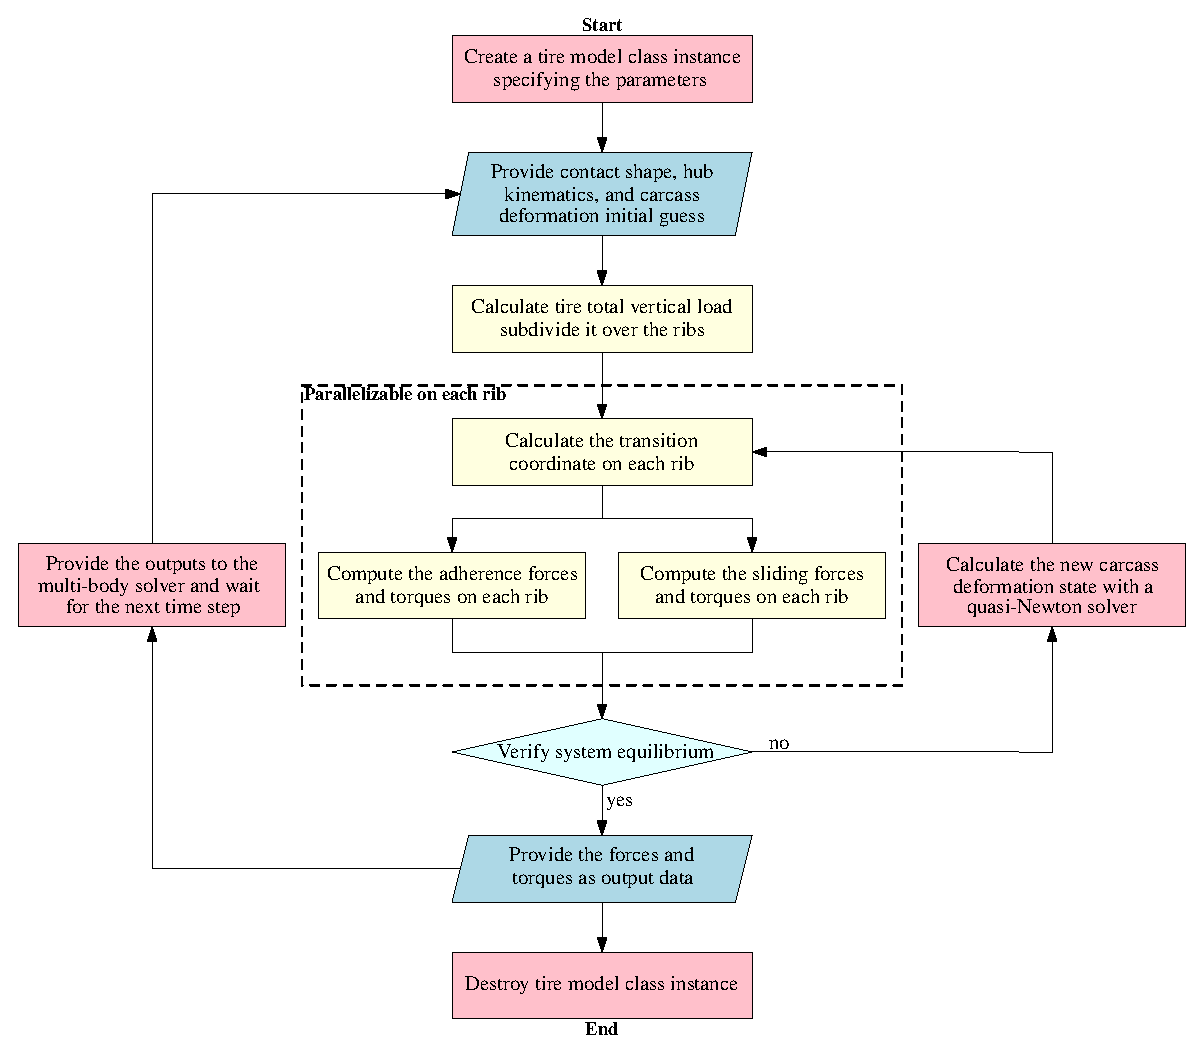
\includegraphics[angle=90, width=0.9\columnwidth]{flowchart}
  \caption{Flowchart of the index reduction algorithm.}
  \label{chap6:fig:index_reduction}
\end{figure}

\begin{algorithm}[H]
  \caption{Index reduction algorithm.}
  \label{chap6:alg:index_reduction}
  \begin{algorithmic}[1]
    \State \textbf{Require:} A \ac{DAE} system of the form $\mF \overset{\mathrm{def}}{=} \mA \, \mxp - \mb = \m{0}$.
    \Procedure{ReduceIndex}{$\mF$} \Comment{Index reduction procedure}
      \State $\mh \gets \varnothing$ \Comment{The set of invariants}
      \State $\mA, \, \mb \gets \mathrm{GenerateMatrix}(\mF, \, \mxp)$ \Comment{The \ac{DAE} system matrix}
      \State $m \gets \mathrm{Size}(\mx)$\Comment{The size of $\mx$}
      \While{$\mA$ is singular}
        \State $\displaystyle\triangleright$ Differential and algebraic equations separation (Section~\ref{chap6:sec:separation})
        \State $\mL, \, \mU, \, \mP, \, \mQ \gets \mathrm{MatrixFactorization}(\mA)$ \Comment{LU or FFLU decomposition of $\mA$}
        \State $r \gets \mathrm{Rank}(\mU)$ \Comment{The rank of $\mU$ is equal to the rank of $\mA$}
        \State $\mI_1 \gets \mathrm{IdentityMatrix}(r, \, r)$ \Comment{The upper identity matrix}
        \State $\mI_2 \gets \mathrm{IdentityMatrix}(m-r, \, m-r)$ \Comment{The lower identity matrix}
        \State $\mE \gets [\mI_1, \, \m{0}] \, \mU \, \mQ^\top$ \Comment{The reordered part of $\mA$}
        \State $\mg \gets [\mI_1, \, \m{0}] \, \mL^{-1} \, \mP \, \mb$ \Comment{The differential part of $\mb$}
        \State $\ma \gets [\m{0}, \, \mI_2] \, \mL^{-1} \, \mP \, \mb$ \Comment{The algebraic part of $\mb$}
        \State
        \State $\displaystyle\triangleright$ Algebraic equations differentiation (Section~\ref{chap6:sec:differentiation})
        \State $\mAd, \, \mgd \gets \mathrm{GenerateMatrix}(\mathrm{Diff}(\ma, \, t), \, \mxp)$ \Comment{Differentiate the equations $\ma$}
        \State $\mA \gets \begin{bmatrix} \mE \\ \mAd \end{bmatrix}$ \quad and \quad $\mb \gets \begin{bmatrix}\mg \\ \mgd \end{bmatrix}$
        \Comment{The new matrix $\mA$ and vector $\mb$}
        \State $\mh \gets \mh \cup \ma$ \Comment{Add the algebraic equations to the set of invariants}
      \EndWhile \\
      \Return $\mA, \, \mb, \, \mh$ \Comment{The \acp{DAE} reduced to an \ac{ODE} system with invariants}
    \EndProcedure
  \end{algorithmic}
\end{algorithm}

\subsection{A Step-by-Step Example}
\label{chap6:sec:step_by_step}

Within this Section, we present the step-by-step results of the index reduction algorithm. To do so we exploit a simple non-stiff index-3 problem found in \Wolfram{}~\Mathematica{} documentation~\cite{mathematica}. The initial value problem is defined as follows
%
\begin{equation}
  \label{chap6:eq:index_3}
  \mF = \begin{bmatrix}
    x^{\prime}_{2} - x_{1} - \cos(t) \\
    x^{\prime}_{3} - x_{2} - \sin(t) \\
    x_{3} - \cos(t)
  \end{bmatrix},
\end{equation}
%
with states $\mx = [x_{1}, \, x_{2}, \, x_{3}]^\top$ and initial conditions $\mx_{0} = [-1, \, 0, \, 1]^\top$. Notice that the analytical solution of this problem is $\mx_{exact} = [\sin(t) - 2\cos(t), \, 2\sin(t), \, \cos(t)]^\top$. The index reduction algorithm is applied to the \ac{DAE} system~\eqref{chap6:eq:index_3} and the step-by-step results for the matrices $\mE$, $\mg$, and $\ma$ are reported here below.
%
\begin{equation*}
  \begin{array}{l}
    \text{Index-3 \acp{DAE}:} \quad \mE = \begin{bmatrix} \,
      0 & 1 & 0 \\
      0 & 0 & 1
    \, \end{bmatrix}, \quad
    \mg = \begin{bmatrix} \,
      \sin(t) - x_{1} \\
      \sin(t) - x_{2}
    \, \end{bmatrix}, \quad\quad~~~\,
    \ma = \begin{bmatrix} \,
      \cos(t) - x_{3}
    \, \end{bmatrix}. \\[1.0em]
    %
    \text{Index-2 \acp{DAE}:} \quad \mE = \begin{bmatrix} \,
      0 & 1 & 0 \\
      0 & 0 & 1
    \, \end{bmatrix}, \quad
    \mg = \begin{bmatrix} \,
      \sin(t) - x_{1} \\
      \sin(t) - x_{2}
    \, \end{bmatrix}, \quad\quad~~~\,
    \ma = \begin{bmatrix} \,
      2\sin(t) - x_{2}
    \, \end{bmatrix}. \\[1.0em]
    %
    \text{Index-1 \acp{DAE}:} \quad \mE = \begin{bmatrix} \,
      0 & 0 & 1 \\
      0 & 1 & 0
    \, \end{bmatrix}, \quad
    \mg = \begin{bmatrix} \,
      \sin(t) - x_{2} \\
      \sin(t) - x_{1}
    \, \end{bmatrix}, \quad\quad~~~\,
    \ma = \begin{bmatrix} \,
      \sin(t) - 2\cos(t) - x_{1}
    \, \end{bmatrix}. \\[1.0em]
    %
    \text{Index-0 \acp{DAE}:} \quad \mE = \begin{bmatrix} \,
      0 & 0 & 1 \\
      0 & 1 & 0 \\
      1 & 0 & 0
    \, \end{bmatrix}, \quad
    \mg = \begin{bmatrix} \,
      \sin(t) - x_{2} \\
      \sin(t) - x_{1} \\
      2\sin(t) + \cos(t)
    \, \end{bmatrix}, \quad
    \ma = \varnothing.
  \end{array}
\end{equation*}
%
The final form of the system is an index-0 \acp{DAE} system is then
%
\begin{equation}
  \label{chap6:eq:index_3_reduced}
  \mF = \begin{bmatrix}
    x^{\prime}_{2} - x_{1} - \cos(t) \\
    x^{\prime}_{3} - x_{2} - \sin(t) \\
    x^{\prime}_{1} - \cos(t) - 2\sin(t)
  \end{bmatrix},
  %
  \quad \text{with invariants} \quad
  %
  \mh = \begin{bmatrix}
    \cos(t) - x_{3} \\
    2\sin(t) - x_{2} \\
    \sin(t) - 2\cos(t) - x_{1}
  \end{bmatrix}.
\end{equation}
%
%Although the just presented example is not so complex and relevant for a real validation of the algorithm, it is useful to demonstrate the step-by-step results of the index reduction algorithm. Furthermore, the expression complexities encountered throughout the index reduction algorithm applied to the Index-3 problem are reported below in \tablename{}~\ref{chap6:tab:complexity}.

\subsection{Known Issues}

While the algorithm just presented is relatively straightforward to implement, it does have two major sources of potential issues that are both determined by the technology used and the fundamental theory.
%
\begin{itemize}
    \item \emph{Expression complexity}. Symbolic manipulation often leads to a growth in expression complexity. For this reason, expression simplification may not always be feasible due to software limitations or excessive CPU time demands. Making the algorithm insensitive to expression swell is thus crucial to its effectiveness.
    \item \emph{Numerical stability of symbolic matrix factorization}. The description of the algorithm involves the manipulation of matrices and vectors with either symbolic or mixed symbolic-numeric entries. Ensuring that symbolic matrix factorization maintains numerical stability is a critical requirement of the algorithm. In the case of \ac{LU} decomposition, inadequate pivoting strategies can lead to the generation of singular matrices, which in turn can cause the algorithm to fail~\cite{zhou2005implicit, zhou2007symbolic, giesbrecht2014symbolic}.
\end{itemize}
%
These are the two main points that we acknowledge in the implementation of the algorithm. In the forthcoming sections, each of these matters is discussed in detail, with recommendations on techniques and open-source software solutions that are used to address them.

% % % % % % % % % % % % % % % % % % % % % % % % % % % % % % % % % % % % % % % %

\section{Expression Swell}
\label{chap6:sec:expression_swell}

Symbolic computation software, such as \Maple{}, is capable of handling relatively large symbolic expressions. However, the increase in complexity can significantly slow down the execution of the index reduction algorithm discussed earlier, resulting in unacceptably long CPU times. This phenomenon, known as expression swell, is a primary contributor to the degradation of performance in symbolic computation kernels. Expression swell can be categorized into two types: \emph{inherent} and \emph{intermediate}. The latter occurs when a calculation temporarily generates extensive expressions during intermediate steps, en route to a potentially more compact final result. To mitigate this issue, hierarchical representation techniques offer a solution~\cite{zhou2006hierarchical}. The core concept of this hierarchical representation is to conceal (or \emph{veil}) intricate expressions from the user by employing auxiliary variables referred to as \emph{veil variables} (or \emph{veils}) and reveal (or \emph{unveil}) them only when they become strictly necessary. As an expert reader may have noticed, expression swell is directly linked to expression complexity. Specifically, choosing the right balance between the maximum expression complexity and the number of veiling variables is crucial to prevent expression swell and concurrently avoid excessive veiling. To effectively gauge expression complexity, a metric is necessary, and various definitions are available. While previous works have relied on the \Maple{}'s \texttt{length} function, we adopt a different measure: the computational cost, which is determined through the \texttt{cost} function in the \texttt{codegen} package. This approach, as illustrated in the forthcoming examples, offers insensitivity to the number of characters used to represent the expression internally to the symbolic computation kernel, thus ensuring superior control over the final expression size.

\paragraph{Large Expression Management} Specific modules designed to perform large expression management tasks and help the user handle hierarchical representations have been developed and documented in prior research~\cite{carette2006linear, zhou2007symbolic}. Among these, the \Maple{} module \texttt{LargeExpressions} already fulfills this role effectively. However, we have observed some minor limitations within this module, primarily arising from its user interface choices rather than the core concept or the programming technique employed. Consequently, they have refined it into a new, object-oriented package known as \LEM{}~\cite{lem2023source}. This updated version remains adherent to the original but offers enhanced control and straightforward utilization of veil variables. Notably, the object-oriented aspect allows for the creation of multiple instances of \LEM{} objects, thereby ensuring a sharp separation between veil variables to prevent potential conflicts resulting from improper usage. Examples of expression complexity calculation and large expression management are reported in~\ref{chap6:sec:complexity} and~\ref{chap6:sec:lem} respectively.

% % % % % % % % % % % % % % % % % % % % % % % % % % % % % % % % % % % % % % % %

\section{Matrix Factorization}
\label{chap6:sec:matrix_factorization}

As previously mentioned, matrix factorization is a widely employed technique for addressing linear systems. There are several types of decompositions, each with distinct properties and characteristics. The \ac{LU} decomposition ranks among the most commonly used approaches. In the context of purely numerical matrices, the practice aligns well with the theoretical foundations of the algorithm. However, when dealing with matrices consisting of either symbolic or mixed symbolic-numeric entries, the situation becomes more intricate~\cite{zhou2007symbolic}. In exact symbolic linear algebra scenarios, the cost of each operation during factorization can vary due to uncontrolled expression swell~\cite{zhou2006hierarchical}. Furthermore, the presence of symbolic values hinders the guarantee of numerical stability. Consequently, a key objective is to derive an output format that retains the symbolic structure of the input matrix and ensures numerical stability.

\paragraph{Fill-In} After the \ac{LU} factorization of a sparse matrix $\m{A}$, it is common to observe that the joint non-zeroes pattern of $\m{L}$ and $\m{U}$ exhibit either equal or lower sparsity compared to the original non-zero pattern of $\m{A}$. This phenomenon, known as fill-in, increases the number of algebraic operations required for solving linear systems, thereby diminishing performance. To mitigate this issue, specific reordering algorithms can be applied to minimize the fill-in of the factorized matrix. These algorithms mainly include \emph{nested dissection}~\cite{george1973nested, lipton1979generalized} and \emph{minimum degree}~\cite{markowitz1957elimination, rose1970symmetric} techniques. In this work, the minimum degree algorithm is preferred due to its ease of implementation. Conversely, the nested dissection is not yet considered as it involves working on the system's graph to identify graph separators, which is a less straightforward process in the symbolic case.

\paragraph{Numerical Stability} A crucial concern is ensuring the numerical stability of the symbolic code generated by matrix factorization. This issue is closely tied to \emph{zero-} or \emph{identity-testing} within symbolic expressions. When simplifying an expression is not feasible, the most commonly adopted methods for zero-testing are the probabilistic ones, which rely on the \emph{DeMillo-Lipton-Schwarz-Zippel lemma}~\cite{demillo1978probabilistic, schwartz1980fast, zippel1979probabilistic}.
%
\begin{itemize}
    \item The utilization of \emph{signature functions} involves the verification of equivalent expressions within a multitude of sub-expressions, a process facilitated by \emph{hashing} techniques~\cite{gonnet1984determining, char1984design, gonnet1986results, monagan1994signature}. In \Maple{}, each expression is stored in the simplification table, employing its signature as a key. A unique feature of these signatures is that equivalent expressions share the same signature. It is important to note that not all expressions can have their signatures determined, such as trigonometric expressions, however, opportune coordinates change for signature computation routines can be applied (see~\ref{chap6:sec:signature}).
    %
    \item The \emph{Hybrid symbolic-numerical} or \emph{static pivoting approach} offers a means to validate the stability of symbolic code through random numerical evaluations~\cite{giesbrecht2014symbolic, li1998making}. While this approach may be computationally less efficient compared to the former method, it yields satisfactory results. In other words, the ``choice of pivots is numerically good at most numerical specializations'' as emphasized in~\cite{giesbrecht2014symbolic}.
\end{itemize}

Based on these observations, the \ac{LU} and \ac{FFLU} factorizations are preferred over the QR and \ac{GJ} factorizations, as the former two involve simpler operations, thereby mitigating the issue of expression swell. Additionally, employing the \ac{LU} factorization with a minimum degree pivoting strategy proves superior in reducing fill-in.

\subsection{Improved Symbolic Pivoting Strategy}

A crucial detail of any \ac{LU}-based decomposition, either numerical or symbolic, is the pivoting strategy. This strategy hinges on the two aforementioned considerations: the degrees of the elements within the system matrix and the actual complexity of the expressions. The elements in the system matrix are arranged in descending order of their degrees, and the pivot of the least complexity is chosen. Sometimes these two features are conflicting. In such cases, the prioritization of the pivot with the lowest degree is preferred. It is important to notice that pivots consisting of numerical values take precedence over those with symbolic values, primarily due to their inherent minimum expression complexity. Throughout the pivoting process, the utilization of signatures is also employed whenever possible to confirm the presence of null expressions without the need for simplification. To summarize, the main steps of the pivoting strategy are the following.
%
\begin{enumerate}
  \item The degree for each of the system matrix's entries is calculated.
  \item The pivots are sorted by degree and a permutation is generated.
  \item The pivots are iterated in the order of the permutation and a candidate pivot is selected at each step.
  \item The candidate pivot is checked for null expressions with the aid of signatures.
  \item If the candidate pivot signature is not null, the expression is simplified and their complexity is calculated.
  \item If the candidate pivot is numeric, its numerical value is calculated, otherwise, it is set to infinity.
  \item The candidate pivot with the lowest complexity or largest absolute numeric value is selected as the best pivot and returned.
\end{enumerate}
%
A detailed description of the developed symbolic pivoting strategy is presented in Algorithm~\ref{chap6:alg:pivoting_strategy}.

\begin{algorithm}[H]
  \caption{Symbolic Pivoting Strategy.}
  \label{chap6:alg:pivoting_strategy}
  \begin{algorithmic}[1]
    \State \textbf{Require:} A $n \times m$ matrix $\m{A}$.
    \State \phantom{\textbf{Require:}} The $k$-th pivoting stage.
    \Procedure{SymbolicPivoting}{$\m{A}$, $k$} \Comment{Symbolic pivoting procedure for the $k$-th pivot}
    \State $\m{d}^r, \, \m{d}^c \gets \text{ComputeDegrees}(\m{A})$ \Comment{Calculate the row and column degrees of $\m{A}$}
    \For{$i$ \textbf{from} $k$ \textbf{to} $n$} \Comment{Iterate over the rows}
      \For{$j$ \textbf{from} $k$ \textbf{to} $m$} \Comment{Iterate over the columns}
        \State $D_{ij} \gets \infty$ \Comment{Set the combined degree matrix to infinity}
        \IfThen{$A_{ij} \neq 0$}
        {$D_{ij} \gets d^r_{i} \, \max(0, \, d^c_j-1) + d^c_j \, \max(0, \, d^r_i-1)$} \Comment{Compute the combined degree}
      \EndFor
    \EndFor
    \State $\mathcal{P} \gets \text{Sort}(\m{D})$ \Comment{Find the permutation that sorts the pivots list by degree cost}
    \State $q, \, l \gets \, 0, \, 0$ \Comment{Initialize the temporary pivot row and column indices}
    \State $p, \, p_c, \, p_n \gets \infty, \, \infty, \, \infty$ \Comment{Initialize the temporary pivot value, complexity and numerical value}
    \For{\textbf{all} $(i, j)$ \textbf{in} $\mathcal{P}$} \Comment{Iterate on the permutation set}
      \IfThen{$p_c \neq \infty$ \textbf{and} $D_{ij} > D_{ql}$}{\textbf{break}} \Comment{No more good pivots to check}
      \State $t \gets A_{ij}$ \Comment{Get the pivot value}
      \IfThen{$\text{Signature}(t) = 0$}{\textbf{continue}} \Comment{Skip the next pivot}
      \State $t \gets \text{Simplify}(t)$ \Comment{Try to simplify the pivot expression}
      \State $t_c \gets \text{ExpressionComplexity}(t)$ \Comment{Calculate the computational complexity of the pivot}
      \State $t_n \gets \infty$ \Comment{Set the default numerical value of the pivot to infinity}
      \IfThen{$t$ is numeric}{$t_n \gets \max(1, \, \mathrm{abs}(t))$} \Comment{Set the numerical value of the pivot}
      \If{$t_c < p_c$ \textbf{or} ($t_c = p_c$ \textbf{and} $t_n > p_n$)} \Comment{If the pivot is better than the current one}
        \State $q, \, l \gets i, \, j$ \Comment{Update the best pivot row and column indices}
        \State $p, \, p_c, \, p_n \gets t, \, t_c, \, t_n$ \Comment{Update the best pivot value, complexity and numerical value}
      \EndIf
    \EndFor \\
    \Return $p, \, q, \, l$ \Comment{The $k$-th pivot and its position}
    \EndProcedure
  \end{algorithmic}
\end{algorithm}

\paragraph{Symbolic Linear Algebra} The considerations outlined above aid as the foundations for the \LAST{} package~\cite{last2023source}. Within this package, the pivoting process has been designed to address the critical considerations of expression swell and numerical stability as previously discussed. This toolkit, integrated into the \Maple{} environment, is dedicated to symbolic linear algebra tasks. It builds upon the original research outlined in~\cite{zhou2008fraction} and encompasses a collection of functionalities for symbolic full-pivoting \ac{LU}, \ac{FFLU}, QR, and \ac{GJ} factorizations. Importantly, the \LAST{} package is intended to be used in tandem with the previously presented \LEM{} package~\cite{lem2023source}, contributing to the mitigation of expression swell.

% % % % % % % % % % % % % % % % % % % % % % % % % % % % % % % % % % % % % % % %

\section{Symbolic-Numerical Examples}
\label{chap6:sec:examples}

In this section, we showcase examples of high-index \ac{DAE} systems, which range in a wide spectrum, encompassing physical systems, engineering applications, as well as ``artificial'' \ac{DAE} systems with specific properties. These examples are employed to demonstrate the capabilities of the proposed index reduction algorithm. In particular, the following test cases are presented.
%
\begin{enumerate}
  \item A non-stiff index-3 problem found in \Wolfram{}~\Mathematica{} documentation~\cite{mathematica}, already showcased in Section~\ref{chap6:sec:step_by_step}.
  \item An index-3 problem with analytical solution, which describes the motion of a particle in 3D~\cite{campbell1995constraint}.
  \item A moderately stiff car-axis problem of index-3 describing a simple model of a car axis riding over a bumpy road~\cite{lioen1998test, mazzia2008test}.
  \item A slightly stiff index-1 system of an eight-nodes transistor-amplifier~\cite{lioen1998test, mazzia2008test}.
  \item A stiff index-2 system of an electric ring modulator~\cite{lioen1998test, mazzia2008test}.
  \item A dimension 5 Rei{\ss}ig's family \ac{DAE} system of index-1~\cite{reissig2000differential}.
  \item An index-3 system that describes the space shuttle reentry problem~\cite{brenan1995numerical}.
  \item An index-5 \ac{DAE} system, which describes the motion of a robotic arm~\cite{pryce1998solving}.
  \item The $\mathrm{N}$-Pendula with: (a)~$\mathrm{N} = 2$ and index-5~\cite{pryce1998solving}; (b)~$\mathrm{N} = 3$ and index-7~\cite{nedialkov2008solvingIII}; and (c)~$\mathrm{N} = 4$ and index-9~\cite{nedialkov2008solvingIII}.
\end{enumerate}
%
Examples 1 and 2 are accurately showcased in Sections~\ref{chap6:sec:step_by_step} and~\ref{chap6:sec:numerical_integration}, respectively. In specific, the first example demonstrates the step-by-step results of the index reduction algorithm presented here, while the second is used to visualize the numerical integration results of the reduced-index system, as well as the good conditioning of both the symbolic matrix factorization and the numerical integration scheme. The remaining tests are presented more concisely, and the expressions' complexity met during the index reduction process for each test is reported in \tablename{}~\ref{chap6:tab:complexity} of Section~\ref{chap6:sec:daes_complexity}. Similarly, the numerical results of the reduced-index systems are reported in \tablename{}~\ref{chap6:tab:numerical_integration} of Section~\ref{chap6:sec:numerical_integration}.

\subsection{Expression Complexity of the Reduced-Index Systems}
\label{chap6:sec:daes_complexity}

To demonstrate the capabilities of the proposed index reduction algorithm, we first consider the examples from a symbolic computation perspective. In particular, we consider the computational cost of the expressions generated during the presented procedure. The compactness of the expressions generated during the index reduction algorithm is a crucial aspect, as it ensures that limited computational overhead is introduced in the numerical integration of the reduced-index system, as well as in the projection of the solution on the hidden constraints. For each reduction stage of the examples considered, the computational cost is reported in \tablename{}~\ref{chap6:tab:complexity}. Notice that the computational costs of expressions that could not be simplified by \Maple{} within \SI{100}{\second} of CPU time are reported with a $\star$ symbol preceding them. The tests are performed on a \SI{2.6}{\giga\hertz} 6-Core Intel\textsuperscript{\textregistered} Core\textsuperscript{\textregistered} i7 computer.

The presented algorithm can successfully reduce the index of all the example \ac{DAE} systems here considered. The computational cost of the expressions generated during the index reduction procedure is comparable to the original \ac{DAE} system in most of the tests. However, it is important to highlight that in examples 7, 8 and 9c some of the expressions generated during the index reduction procedure are significantly more complex than the original \ac{DAE} system. In these cases, the \Maple{} symbolic computation kernel is not able to perform the simplification within \SI{100}{\second} of CPU time and the raw expressions are kept in the following reduction steps. As a consequence, the computational cost inherently increases throughout the following reduction steps. The \ac{DAE} systems that are hard to simplify are those having a matrix $\mA$ that is strongly dependent on the state variables $\mx$ or equivalently that retains complicated divisions in the vector $\mb$. In these cases, the computational cost of the vector $\ma$ increases significantly due to successive and repeated differentiation and symbolic factorization. The trigonometric identities provided by Weierstra{\ss}~\eqref{chap6:eq:weierstrass} or~\eqref{chap6:eq:zhou} can be used to obtain polynomial expressions and improve the detection of symbolic eliminations (see~\ref{chap6:sec:signature}). However, the use of such trigonometric identities does not typically lead to a significant improvement in the computational cost of the expressions generated during the index reduction procedure as the polynomial expressions obtained are hard to simplify as well.

Another aspect that is important to mention is the sudden increase in computational complexity of the expressions generated in the last reduction step. Even if this increase is not critical to the correct index reduction as the presented algorithm is robust to expression swell, it does undermine the numerical efficiency of the final \ac{DAE} system. This highlights the need for further research on expression swell mitigation techniques in symbolic computation (see~\ref{chap6:sec:lem}), as well as the need to use integrators that can handle index-1 or even index-2 \acp{DAE}.

\setlength\tabcolsep{0.0pt}
\setlength{\LTcapwidth}{\textwidth}
{\footnotesize\centering\begin{longtable}{cccc}
  \caption[
    Expression complexity encountered throughout the index reduction algorithm of the test \ac{DAE} systems.
  ]{
    Expression complexity encountered throughout the index reduction algorithm of the test \ac{DAE} systems. \emph{Legend}: $\cf$ = functions, $\ca$ = additions, $\cm$ = multiplications, and $\cd$ = divisions. Expressions preceded by the $\star$ symbol could not be simplified within \SI{100}{\second} of CPU time in the \Maple{} environment.
  }
  \label{chap6:tab:complexity}
  \endfirsthead
  \endhead
  %
  \multicolumn{4}{c}{\textbf{1.~~Index-3 \acp{DAE}~\cite{mathematica}}} \\
  \toprule
  \textbf{Original \acp{DAE}} & \multicolumn{3}{c}{$\mF = 10\cf + 5\ca$ \quad $\mh = 0$} \\
  \midrule
  \textbf{Reduction step} & $\mE$ & $\mg$ & $\ma$ \\
  \midrule
  Index-3 \acp{DAE} & 0 & $4\cf + 2\ca$ & $2\cf + 1\ca$ \\
  Index-2 \acp{DAE} & 0 & $4\cf + 2\ca$ & $2\cf + 1\cm + 1\ca$ \\
  Index-1 \acp{DAE} & 0 & $4\cf + 2\ca$ & $3\cf + 1\cm + 1\ca$ \\
  Index-0 \acp{DAE} & 0 & $6\cf + 1\cm + 3\ca$ & $0$ \\
  \midrule
  \textbf{Reduced \acp{DAE}} & \multicolumn{3}{c}{$\mF = 12\cf + 1\cm + 6\ca$ \quad $\mh = 7\cf + 2\cm + 4\ca$} \\
  \bottomrule \\[-0.1em]
  %
  \multicolumn{4}{c}{\textbf{2.~~Particle Motion~\cite{campbell1995index}}} \\
  \toprule
  \textbf{Original \acp{DAE}} & \multicolumn{3}{c}{$\mF = 47\cf + 30\cm + 23\ca$ \quad $\mh = 0$} \\
  \midrule
  \textbf{Reduction step} & $\mE$ & $\mg$ & $\ma$ \\
  \midrule
  Index-3 \acp{DAE} & 0 & $39\cf + 36\cm + 13\ca$ & $7\cf + 10\cm + 6\ca$ \\
  Index-2 \acp{DAE} & 0 & $39\cf + 36\cm + 13\ca$ & $22\cf + 20\cm + 8\ca$ \\
  Index-1 \acp{DAE} & 0 & $39\cf + 36\cm + 13\ca$ & $68\cf + 72\cm + 33\ca$ \\
  Index-0 \acp{DAE} & $388\cf + 424\cm + 180\ca$ & $79\cf + 77\cm + 26\ca$ & 0 \\
  \midrule
  \textbf{Reduced \acp{DAE}} & \multicolumn{3}{c}{$\mF = 258\cf + 239\cm + 109\ca$ \quad $\mh = 97\cf + 102\cm + 47\ca$} \\
  \bottomrule \\[-0.1em]
  %
  \multicolumn{4}{c}{\textbf{3.~~Car-Axis~\cite{lioen1998test, mazzia2008test}} } \\
  \toprule
  \textbf{Original \acp{DAE}} & \multicolumn{3}{c}{$\mF = 108\cf + 131\cm + 56\ca$ \quad $\mh = 0$} \\
  \midrule
  \textbf{Reduction step} & $\mE$ & $\mg$ & $\ma$ \\
  \midrule
  Index-3 \acp{DAE} & $12\cm$ & $94\cf + 145\cm + 54\ca$ & $14\cf + 16\cm + 10\ca$ \\
  Index-2 \acp{DAE} & $12\cm$ & $94\cf + 145\cm + 54\ca$ & $26\cf + 45\cm + 15\ca$ \\
  Index-1 \acp{DAE} & $12\cm$ & $94\cf + 145\cm + 54\ca$ & $136\cf + 4\cd + 261\cm + 95\ca$ \\
  Index-0 \acp{DAE} & $1060\cf + 38\cd + 1901\cm + 717\ca$ & $431\cf + 8\cd + 842\cm + 268\ca$ & 0 \\
  \midrule
  \textbf{Reduced \acp{DAE}} & \multicolumn{3}{c}{$\mF = 896\cf + 4\cd + 1202\cm + 546\ca$ \quad $\mh = 176\cf + 4\cd + 322\cm + 120\ca$} \\
  \bottomrule \\[-0.1em]
  %
  \multicolumn{4}{c}{\textbf{4.~~Eight-Nodes Transistor-Amplifier~\cite{lioen1998test, mazzia2008test}}} \\
  \toprule
  \textbf{Original \acp{DAE}} & \multicolumn{3}{c}{$\mF = 55\cf + 21\cd + 29\cm + 41\ca$ \quad $\mh = 0$} \\
  \midrule
  \textbf{Reduction step} & $\mE$ & $\mg$ & $\ma$ \\
  \midrule
  Index-1 \acp{DAE} & $5\ca$ & $17\cf + 11\cd + 22\cm + 20\ca$ & $19\cf + 12\cd + 44\cm + 24\ca$ \\
  Index-0 \acp{DAE} & $24\cf + 26\cd + 24\cm + 24\ca$ & $18\cf + 12\cd + 26\cm + 20\ca$ & 0 \\
  \midrule
  \textbf{Reduced \acp{DAE}} & \multicolumn{3}{c}{$\mF = 74\cf + 26\cd + 87\cm + 49\ca$ \quad $\mh = 19\cf + 12\cd + 44\cm + 26\ca$} \\
  \bottomrule \\[-0.1em]
  %
  \multicolumn{4}{c}{\textbf{5.~~Electric Ring Modulator~\cite{lioen1998test, mazzia2008test}}} \\
  \toprule
  \textbf{Original \acp{DAE}} & \multicolumn{3}{c}{$\mF = 116\cf + 3\cd + 75\cm + 92\ca$ \quad $\mh = 0$} \\
  \midrule
  \textbf{Reduction step} & $\mE$ & $\mg$ & $\ma$ \\
  \midrule
  Index-2 \acp{DAE} & $0$ & $51\cf + 3\cd + 41\cm + 41\ca$ & $44\cf + 32\cm + 36\ca$ \\
  Index-1 \acp{DAE} & $86\cf + 68\cm + 66\ca$ & $262\cf + 13\cd + 416\cm + 220\ca$ & $10\cf + 2\cd + 18\cm + 11\ca$ \\
  Index-0 \acp{DAE} & $86\cf + 12\cd + 72\cm + 70\ca$ & $262\cf + 13\cd + 416\cm + 220\ca$ & 0 \\
  \midrule
  \textbf{Reduced \acp{DAE}} & \multicolumn{3}{c}{$\mF = 335\cf + 15\cd + 537\cm + 256\ca$ \quad $\mh = 54\cf + 2\cd + 50\cm + 47\ca$} \\
  \bottomrule \\[-0.1em]
  %
  \multicolumn{4}{c}{\textbf{6.~~Rei{\ss}ig's \acp{DAE}~\cite{reissig2000differential}}} \\
  \toprule
  \textbf{Original \acp{DAE}} & \multicolumn{3}{c}{$\mF = 13\cf + 26\ca$ \quad $\mh = 0$} \\
  \midrule
  \textbf{Reduction step} & $\mE$ & $\mg$ & $\ma$ \\
  \midrule
  Index-1 \acp{DAE} & $0$ & $4\cf + 2\ca$ & $10\cf + 5\ca$ \\
  Index-0 \acp{DAE} & $0$ & $14\cf + 5\ca$ & 0 \\
  \midrule
  \textbf{Reduced \acp{DAE}} & \multicolumn{3}{c}{$\mF = 32\cf + 13\ca$ \quad $\mh = 10\cf + 7\ca$} \\
  \bottomrule \\[-0.1em]
  %
  \multicolumn{4}{c}{\textbf{7.~~Space Shuttle Reentry~\cite{brenan1995numerical}}} \\
  \toprule
  \textbf{Original \acp{DAE}} & \multicolumn{3}{c}{$\mF = 116\cf + 16\cd + 77\cm + 38\ca$ \quad $\mh = 0$} \\
  \midrule
  \textbf{Reduction step} & $\mE$ & $\mg$ & $\ma$ \\
  \midrule
  Index-3 \acp{DAE} & $0$ & $112\cf + 13\cd + 247\cm + 49\ca$ & $6\cf + 1\cd + 30\cm + 11\ca$ \\
  Index-2 \acp{DAE} & $0$ & $112\cf + 13\cd + 247\cm + 49\ca$ & $66\cf + 2\cd + 529\cm + 123\ca$ \\
  Index-1 \acp{DAE} & $0$ & $112\cf + 13\cd + 247\cm + 49\ca$ & $903\cf + 4\cd + 8382\cm + 1369\ca$ \\
  Index-0 \acp{DAE} & $5612\cf + 28\cd + 50347\cm + 8204\ca$ & $112\cf + 13\cd + 247\cm + 49\ca$ & 0 \\
  \midrule
  \textbf{Reduced \acp{DAE}} & \multicolumn{3}{c}{$\star \mF = 5749\cf + 41\cd + 50599\cm + 8263\ca$ \quad $\mh = 975\cf + 7\cd + 8941\cm + 1503\ca$} \\
  \bottomrule \\[-0.1em]
  %
  \multicolumn{4}{c}{\textbf{8.~~Robotic Arm~\cite{pryce1998solving}}} \\
  \toprule
  \textbf{Original \acp{DAE}} & \multicolumn{3}{c}{$\mF = 125\cf + 19\cd + 56\cm + 64\ca$ \quad $\mh = 0$} \\
  \midrule
  \textbf{Reduction step} & $\mE$ & $\mg$ & $\ma$ \\
  \midrule
  Index-5 \acp{DAE} & $0$ & $66\cf + 3\cd + 50\cm + 35\ca$ & $16\cf + 12\ca$ \\
  Index-4 \acp{DAE} & $0$ & $66\cf + 3\cd + 50\cm + 35\ca$ & $24\cf + 6\cm + 14\ca$ \\
  Index-3 \acp{DAE} & $0$ & $66\cf + 3\cd + 50\cm + 35\ca$ & $162\cf + 2\cd + 138\cm + 114\ca$ \\
  Index-2 \acp{DAE} & $14\cf + 2\cd + 6\cm + 6\ca$ & $372\cf + 4\cd + 375\cm + 253\ca$ & $972\cf + 1\cd + 1062\cm + 770\ca$ \\
  Index-1 \acp{DAE} & $14\cf + 2\cd + 6\cm + 6\ca$ & $372\cf + 4\cd + 375\cm + 253\ca$ & $\star (6.5\cf + 5.6\cm + 1.8\ca)\cdot10^{6} + 4\cd$ \\
  Index-0 \acp{DAE} & $\star (8.3\cf + 7.1\cm + 2.3\ca)\cdot10^{7} + 58\cd$ & $(2.4\cf + 2.0\cm + 0.9\ca)\cdot10^{6} + 8\cd$ & 0 \\
  \midrule
  \textbf{Reduced \acp{DAE}} & \multicolumn{3}{c}{$\star \mF = (8.6\cf + 7.3\cm + 2.4\ca)\cdot10^{7} + 66\cd$ \quad $\star \mh = (6.5\cf + 5.6\cm + 1.8\ca)\cdot10^{6} + 7\cd$} \\
  \bottomrule \\[-0.1em]
  %
  \multicolumn{4}{c}{\textbf{9a.~~2-Pendula~\cite{pryce1998solving}}} \\
  \toprule
  \textbf{Original \acp{DAE}} & \multicolumn{3}{c}{$\mF = 67\cf + 31\cm + 31\ca$ \quad $\mh = 0$} \\
  \midrule
  \textbf{Reduction step} & $\mE$ & $\mg$ & $\ma$ \\
  \midrule
  Index-5 \acp{DAE} & $0$                  & $12\cf + 8\cm + 2\ca$ & $6\cf + 12\cm + 6\ca$ \\
  Index-4 \acp{DAE} & $1\cf + 5\cm + 1\ca$ & $16\cf + 12\cm + 3\ca$ & $4\cf + 4\cm + 1\ca$ \\
  Index-3 \acp{DAE} & $1\cf + 5\cm + 1\ca$ & $16\cf + 12\cm + 3\ca$ & $7\cf + 12\cm + 4\ca$ \\
  Index-2 \acp{DAE} & $1\cf + 5\cm + 1\ca$ & $16\cf + 12\cm + 3\ca$ & $18\cf + 2\cd + 30\cm + 9\ca$ \\
  Index-1 \acp{DAE} & $1\cf + 5\cm + 1\ca$ & $16\cf + 12\cm + 3\ca$ & $118\cf + 2\cd + 283\cm + 72\ca$ \\
  Index-0 \acp{DAE} & $555\cf + 21\cd + 1213\cm + 287\ca$ & $16\cf + 12\cm + 3\ca$ & $0$ \\
  \midrule
  \textbf{Reduced \acp{DAE}} & \multicolumn{3}{c}{
  $\mF = 482\cf + 2\cd + 807\cm + 229\ca$ \quad $\mh = 153\cf + 4\cd + 341\cm + 92\ca$} \\
  \bottomrule \\[-0.1em]
  %
  \multicolumn{4}{c}{\textbf{9b.~~3-Pendula~\cite{nedialkov2008solvingIII}}} \\
  \toprule
  \textbf{Original \acp{DAE}} & \multicolumn{3}{c}{$\mF = 67\cf + 31\cm + 31\ca$ \quad $\mh = 0$} \\
  \midrule
  \textbf{Reduction step} & $\mE$ & $\mg$ & $\ma$ \\
  \midrule
  Index-7 \acp{DAE} & $0$                   & $18\cf + 12\cm + 3\ca$ & $10\cf + 21\cm + 10\ca$ \\
  Index-6 \acp{DAE} & $2\cf + 10\cm + 2\ca$ & $26\cf + 20\cm + 5\ca$ & $4\cf + 4\cm + 1\ca$ \\
  Index-5 \acp{DAE} & $2\cf + 10\cm + 2\ca$ & $26\cf + 20\cm + 5\ca$ & $4\cf + 12\cm + 7\ca$ \\
  Index-4 \acp{DAE} & $2\cf + 10\cm + 2\ca$ & $26\cf + 20\cm + 5\ca$ & $18\cf + 2\cd + 30\cm + 9\ca$ \\
  Index-3 \acp{DAE} & $2\cf + 10\cm + 2\ca$ & $26\cf + 20\cm + 5\ca$ & $118\cf + 2\cd + 283\cm + 72\ca$ \\
  Index-2 \acp{DAE} & $2\cf + 10\cm + 2\ca$ & $26\cf + 20\cm + 5\ca$ & $992\cf + 3\cd + 2077\cm + 479\ca$ \\
  Index-1 \acp{DAE} & $2\cf + 10\cm + 2\ca$ & $26\cf + 20\cm + 5\ca$ & $6824\cf + 3\cd + 17665\cm + 4030\ca$ \\
  Index-0 \acp{DAE} & $54152\cf + 51\cd + 136388\cm + 28945\ca$ & $26\cf + 20\cm + 5\ca$ & $0$ \\
  \midrule
  \textbf{Reduced \acp{DAE}} & \multicolumn{3}{c}{
  $\mF = 28319\cf + 3\cd + 64295\cm + 15806\ca$ \quad $\mh = 7973\cf + 10\cd + 20092\cm + 4605\ca$} \\
  \bottomrule \\[-0.1em]
  %
  \multicolumn{4}{c}{\textbf{9c.~~4-Pendula~\cite{nedialkov2008solvingIII}}} \\
  \toprule
  \textbf{Original \acp{DAE}} & \multicolumn{3}{c}{$\mF = 67\cf + 31\cm + 31\ca$ \quad $\mh = 0$} \\
  \midrule
  \textbf{Reduction step} & $\mE$ & $\mg$ & $\ma$ \\
  \midrule
  Index-9 \acp{DAE} & $0$                   & $24\cf + 16\cm + 4\ca$ & $14\cf + 30\cm + 14\ca$ \\
  Index-8 \acp{DAE} & $3\cf + 15\cm + 3\ca$ & $36\cf + 28\cm + 7\ca$ & $4\cf + 4\cm + 1\ca$ \\
  Index-7 \acp{DAE} & $3\cf + 15\cm + 3\ca$ & $36\cf + 28\cm + 7\ca$ & $7\cf + 12\cm + 4\ca$ \\
  Index-6 \acp{DAE} & $3\cf + 15\cm + 3\ca$ & $36\cf + 28\cm + 7\ca$ & $18\cf + 2\cd + 30\cm + 9\ca$ \\
  Index-5 \acp{DAE} & $3\cf + 15\cm + 3\ca$ & $36\cf + 28\cm + 7\ca$ & $118\cf + 2\cd + 283\cm + 72\ca$ \\
  Index-4 \acp{DAE} & $3\cf + 15\cm + 3\ca$ & $36\cf + 28\cm + 7\ca$ & $992\cf + 3\cd + 2077\cm + 479\ca$ \\
  Index-3 \acp{DAE} & $3\cf + 15\cm + 3\ca$ & $36\cf + 28\cm + 7\ca$ & $6824\cf + 3\cd + 17665\cm + 4030\ca$ \\
  Index-2 \acp{DAE} & $3\cf + 15\cm + 3\ca$ & $36\cf + 28\cm + 7\ca$ & $(4.8\cf + 4\cd + 11.9\cm + 2.7\ca)\cdot10^{5}$ \\
  Index-1 \acp{DAE} & $3\cf + 15\cm + 3\ca$ & $36\cf + 28\cm + 7\ca$ & $\star (3.0\cf + 14.9\cm + 0.4\ca)\cdot10^{6} + 4\cd$ \\
  Index-0 \acp{DAE} & $\star (3.0\cf + 14.7\cm + 0.4\ca)\cdot10^{7} + 92\cd$ & $7\cf + 28\cm + 36\ca$ & 0 \\
  \midrule
  \textbf{Reduced \acp{DAE}} & \multicolumn{3}{c}{
  $\star \mF = (3.0\cf + 14.7\cm + 0.4\ca)\cdot10^{7} + 92\cd$ \quad $\star \mh = (3.1\cf + 15.1\cm + 0.5\ca)\cdot10^{6} + 18\cd$} \\
  \bottomrule
  %
\end{longtable}}

\subsection{Numerical Integration of the Reduced-Index System}
\label{chap6:sec:numerical_integration}

To demonstrate the numerical stability of the reduced-index system, we consider the second example, which is an index-3 problem with an analytical solution, taken from~\cite{campbell1995constraint}. It describes the motion of a particle inside a 3D torus surface. This system has three position variables $[x_{1}, \, x_{2}, \, x_{3}]^\top$, three velocity variables $[u_{1}, \, u_{2}, \, u_{3}]^\top$, and one constraint with Lagrange multiplier $\lambda$. The solution manifold is 4D, and the exact solution is
%
\begin{equation}
  \label{chap6:eq:torus_solution}
  \mx_{exact} = \begin{bmatrix}
    x_{1} \\ x_{2} \\ x_{3}
  \end{bmatrix} = \begin{bmatrix}
    (\rho \cos(2\pi - t) + r) \cos(t) \\
    (\rho \cos(2\pi - t) + r) \sin(t) \\
    \rho \sin(2\pi - t)
  \end{bmatrix}.
\end{equation}
%
The initial value problem is defined as follows
%
\begin{equation}
  \label{chap6:eq:torus}
  \mF = \begin{bmatrix}
    x^{\prime}_{1} - u_{1} \\
    x^{\prime}_{2} - u_{2} \\
    x^{\prime}_{3} - u_{3} \\
    u^{\prime}_{1} - u_{3}\cos(t) + x_{3}\sin(t) + u_{2} - 2 c x_{1}\lambda \\
    u^{\prime}_{2} - u_{3}\sin(t) - x_{3}\cos(t) - u_{1} - 2 c x_{2}\lambda \\
    u^{\prime}_{3} + x_{3} - 2x_{3}\lambda \\
    x_{1}^2 + x_{2}^2 + x_{3}^2 - 2r(x_{1}^2 + x_{2}^2)^{1/2} + r^2 - \rho^2
  \end{bmatrix},
\end{equation}
%
with $c = 1 - {r} / {(x_{1}^2 + x_{2}^2)^{1/2}}$, states $\mx = [x_{1}, \, x_{2}, \, x_{3}, \, u_{1}, \, u_{2}, \, u_{3}, \, \lambda]^{\top}$, initial conditions $\mx_{0} = [15, \, 0, \, 0, \, 0, \, 15, \, -5, \, \lambda]^{\top}$, and parameters $\rho = 5$ and $r = 10$. The index reduction algorithm is applied to the \ac{DAE} system and reduced to index-0. The expressions' complexity of the step-by-step results are reported in \tablename{}~\ref{chap6:tab:complexity}.

The numerical integration of the reduced-index system is performed through Implicit Euler, RadauIIA3, and RadauIIA5 Runge-Kutta methods. To respect the invariants during the integration the \emph{standard projection} method is applied \cite{hairer2000symmetric}. This method consists of projecting the solution $\mx$ of the numerically integrated system onto the invariants on the hidden constraints $\mh = \m{0}$, which is equivalent to the constrained minimization
%
\begin{equation}
  \underset{\tilde{\mx}}{\textrm{minimize}} \quad \dfrac{1}{2}\left(\mx - \tilde{\mx}\right)^2
    \quad \textrm{subject to} \quad
    \mh = \m{0}.
\end{equation}
%
To verify that the projection is performed correctly and does not affect the order of the Runge-Kutta method, numerical integration is performed in the interval $t \in [0, \, 2\pi]$ seconds with different integration time steps $\Delta t$. The error of the numerical integration $\varepsilon = \| \, \mx - \mx_{exact} \, \|_{\infty}$ is reported in \figurename~\ref{chap6:fig:torus_order}. As can be seen, the implemented projection preserves the order of the method for all the integration time steps. It is important to highlight that to obtain such results the absolute error tolerances of the integrator and the projection are both set to $\varepsilon = 10^{-10}$. The same tolerances are used in the numerical integration of the reduced-index system in the interval $t \in [0, \, 400\pi]$ seconds with step $\Delta t = 0.025$ seconds. The results are reported in \figurename~\ref{chap6:fig:torus_integration}, where Implicit Euler, RadauIIA3, and RadauIIA5 Runge-Kutta methods are employed, and the projection on the hidden constraints $\mh$ is performed. The effect of the projection is highlighted on the bottom left plot.

\begin{figure}[htp!]
  \centering
  \includetikz{./figures/chapter_6/torus_order.tex}
  \includetikz{./figures/chapter_6/torus_hidden.tex}
  \caption{Numerical integration error $\varepsilon = \| \, \mx - \mx_{exact} \, \|_{\infty}$ of the \acp{DAE}~\eqref{chap6:eq:torus} over different integration time steps $\Delta t$, along with the computed order of the method (left). The projection on the hidden constraints is performed and the invariants violation $\| \, \mh \, \|_{\infty}$ is reported (right). Notice that the implemented projection preserves the order of the method for all the integration time steps. The tests are performed in the interval $t \in [0, \, 2\pi]$ seconds, using Implicit Euler, RadauIIA3, and RadauIIA5 Runge-Kutta methods.}
  \label{chap6:fig:torus_order}
\end{figure}

\begin{figure}[htp!]
  \centering
  \includetikz{./figures/chapter_6/torus_implicit_euler.tex}
  \includetikz{./figures/chapter_6/torus_radauiia3.tex}
  \includetikz{./figures/chapter_6/torus_radauiia5.tex}
  \includetikz{./figures/chapter_6/torus_radauiia5_noproj.tex}
  \caption{Numerically integrated solution of the \acp{DAE}~\eqref{chap6:eq:torus} in the interval $t \in [0, \, 400\pi]$ seconds, with step $\Delta t = 0.025$ seconds, using Implicit Euler (top left), RadauIIA3 (top right), and RadauIIA5 (bottom left and right) Runge-Kutta methods. The first three plots show the numerical integration of the reduced-index system with projection on the hidden constraints $\mh$ produced by the index reduction algorithm. On the bottom right plot, the numerical integration of the reduced-index system is performed without projection on the manifold $\mh$ and substantial drift is observed.}
  \label{chap6:fig:torus_integration}
\end{figure}

The numerical integration for the remaining examples is also carried out, with outcomes detailed in \tablename{}~\ref{chap6:tab:numerical_integration}. This table reports the performance comparison between the joint index reduction algorithm and numerical integration schemes offered by \Maple{} and those of \Indigo{}. To ensure a fair comparison, both \Maple{} and \Indigo{} utilize the Runge-Kutta-Fehlberg 4(5) method for numerical integration of the \ac{DAE} system. Identical error tolerances are applied, with a relative tolerance of $10^{-6}$ and an absolute tolerance of $10^{-7}$. The results illustrate that the \Indigo{}'s index reduction algorithm implementation effectively generates numerically stable reduced-index \acp{DAE}, ensuring consistent integration across examples. However, exceptions arise in examples 8, 9b, and 9c. In example 8, \Maple{} fails to generate code for the reduced-index system within the expected time frame, thus the integration is not performed. This is due to the complexity of the expressions generated during the index reduction procedure, which overloads the \Maple{}'s \texttt{CodeGeneration} package.
Conversely, in examples 9b and 9c the integration of the reduced-index system is successfully performed using the non-default implicit RadauIIA5 method. Nonetheless, \Maple{}'s \texttt{dsolve} exceeded the function evaluations limit during the numerical integration of example 4 and fails in examples 5, 7, 8, 9b, and 9c due to either system's stiffness or high index.

It is important to highlight that during the numerical integration, the symbolic code is not regenerated by updating the index reduction. Therefore, for some numerical values of states and parameters, the \acp{DAE} system structure may change, leading to numerical instability. While this does pose a potential issue, it is worth noting that we have not encountered instability in the integration process, proving that the presented pivoting strategy is effective.

\setlength\tabcolsep{2.5pt}
\setlength{\LTcapwidth}{\textwidth}
{\footnotesize\centering\begin{longtable}{lccl}
  \caption{Numerical integration results of the reduced-index \ac{DAE} systems. The table reports the name and reference of the \ac{DAE} system, the index of the system, the integration interval $t \in [t_{\text{ini}}, \, t_{\text{end}}]$, and the outcomes of the whole code generation and integration process for both \Maple{} and \Indigo{}. If not otherwise specified, the tests are integrated using a Runge-Kutta-Fehlberg 4(5) method with a relative tolerance of $10^{-6}$ and an absolute tolerance of $10^{-7}$. The computation time limit is \SI{1000}{\second}, to both generate the necessary code and perform numerical computations. \emph{Legend:} \mycheckmark{} successful code generation and numerical integration, \mycrossmark{} errors in the code generation, numerical integration or time expired, and \mywarnmark{} warnings encountered or non-default settings used in the code generation or numerical integration.}
  \label{chap6:tab:numerical_integration}
  \endfirsthead
  \endhead
  %
  \toprule
  \textbf{Integrated \ac{DAE} system} &
  \multicolumn{3}{l}{\textbf{Integration outcomes and errors}} \\
  \midrule
  \multirow{1}{*}{\textbf{1.~~Index-3 \acp{DAE}~\cite{mathematica}}}
    & \Maple{}  & \mycheckmark{}\phantom{\mywarnmark{}} & Success \\ \cmidrule(l{4pt}){2-4}
    Index-3 \quad $t \in [0, 200\pi]$ seconds & \Indigo{} & \mycheckmark{}\phantom{\mywarnmark{}} & Success \\ \midrule
  \multirow{1}{*}{\textbf{2.~~Particle Motion~\cite{campbell1995index}}}
    & \Maple{}  & \mycheckmark{}\phantom{\mywarnmark{}} & Success \\ \cmidrule(l{4pt}){2-4}
    Index-3 \quad $t \in [0, 400\pi]$ seconds & \Indigo{} & \mycheckmark{}\phantom{\mywarnmark{}} & Success \\ \midrule
  \multirow{1}{*}{\textbf{3.~~Car-Axis~\cite{lioen1998test, mazzia2008test}}}
    & \Maple{}  & \mycheckmark{}\phantom{\mywarnmark{}} & Success \\ \cmidrule(l{4pt}){2-4}
    Index-3 \quad $t \in [0, 3]$ seconds & \Indigo{} & \mycheckmark{}\phantom{\mywarnmark{}} & Success \\ \midrule
  \multirow{1}{*}{\textbf{4.~~Eight-Nodes Transistor-Amplifier~\cite{lioen1998test, mazzia2008test}}}
    & \Maple{}  & \mycheckmark{}\mywarnmark{} & Warning, function evaluations limit exceeded \\ \cmidrule(l{4pt}){2-4}
    Index-1 \quad $t \in [0, 0.2]$ seconds & \Indigo{} & \mycheckmark{}\phantom{\mywarnmark{}} & Success \\ \midrule
  \multirow{1}{*}{\textbf{5.~~Electric Ring Modulator~\cite{lioen1998test, mazzia2008test}}}
    & \Maple{}  & \mycrossmark{}\phantom{\mywarnmark{}} & Error, time expired (in \texttt{dsolve}) \\ \cmidrule(l{4pt}){2-4}
    Index-2 \quad $t \in [0, 1]$ milliseconds & \Indigo{} & \mycheckmark{}\phantom{\mywarnmark{}} & Success \\ \midrule
  \multirow{1}{*}{\textbf{6.~~Rei{\ss}ig's \acp{DAE}~\cite{reissig2000differential}}}
    & \Maple{}  & \mycheckmark{}\phantom{\mywarnmark{}} & Success \\ \cmidrule(l{4pt}){2-4}
    Index-1 \quad $t \in [0, 10]$ seconds & \Indigo{} & \mycheckmark{}\phantom{\mywarnmark{}} & Success \\ \midrule
  \multirow{1}{*}{\textbf{7.~~Space Shuttle Reentry~\cite{brenan1995numerical}}}
    & \Maple{}  & \mycrossmark{}\phantom{\mywarnmark{}} & Error, time expired (in \texttt{dsolve}) \\ \cmidrule(l{4pt}){2-4}
    Index-3 \quad $t \in [332.8, 419.8]$ seconds & \Indigo{} & \mycheckmark{}\phantom{\mywarnmark{}} & Success \\ \midrule
  \multirow{1}{*}{\textbf{8.~~Robotic Arm~\cite{pryce1998solving}}}
    & \Maple{}  & \mycrossmark{}\phantom{\mywarnmark{}} & Error, time expired (in \texttt{dsolve}) \\ \cmidrule(l{4pt}){2-4}
    Index-5 \quad $t \in [0, 2]$ seconds & \Indigo{} & \mycrossmark{}\phantom{\mywarnmark{}} & Error, time expired (in \texttt{CodeGeneration}) \\ \midrule
  \multirow{1}{*}{\textbf{9a.~~2-Pendula~\cite{pryce1998solving}}}
    & \Maple{}  & \mycheckmark{}\phantom{\mywarnmark{}} & Success \\ \cmidrule(l{4pt}){2-4}
    Index-5 \quad $t \in [0, 60]$ seconds & \Indigo{} & \mycheckmark{}\phantom{\mywarnmark{}} & Success \\ \midrule
  \multirow{1}{*}{\textbf{9b.~~3-Pendula~\cite{nedialkov2008solvingIII}}}
    & \Maple{}  & \mycrossmark{}\phantom{\mywarnmark{}} & Error, time expired (in \texttt{dsolve}) \\ \cmidrule(l{4pt}){2-4}
    Index-7 \quad $t \in [0, 60]$ seconds & \Indigo{} & \mycheckmark{}\mywarnmark{} & Success with RadauIIA5 method \\ \midrule
  \multirow{1}{*}{\textbf{9c.~~4-Pendula~\cite{nedialkov2008solvingIII}}}
    & \Maple{}  & \mycrossmark{}\phantom{\mywarnmark{}} & Error, time expired (in \texttt{dsolve}) \\ \cmidrule(l{4pt}){2-4}
    Index-9 \quad $t \in [0, 60]$ seconds & \Indigo{} & \mycheckmark{}\mywarnmark{} & Success with RadauIIA5 method \\
  \bottomrule
  %
\end{longtable}}

% % % % % % % % % % % % % % % % % % % % % % % % % % % % % % % % % % % % % % % %

\section{Future Work}
\label{chap6:sec:future_work}

Despite its proven effectiveness, the presented symbolic index reduction algorithm offers scope for various methodological and implementation enhancements, which will be the subject of future research.

\subsection{Improved Pivoting Strategy}

Notably, the symbolic factorization relies on full-pivoting \ac{LU} decomposition. The choice of a pivot strategy holds paramount importance for achieving numerical stability in the reduced-index system. The present implementation selects pivots based on the minimum degree technique and expression complexity to minimize fill-in. However, this metric may not always be effective and the use of nested dissection or other techniques may further reduce fill-in and improve the numerical stability of the solution as well as the overall memory performance of the algorithm.

\subsection{Continued Symbolic Matrix Factorization}

In the present version, the matrix decomposition is repeated throughout the all \ac{DAE} system at every reduction step. This can be avoided by saving the partial factorization of the matrix $\mA$ and continuing it in the following reduction steps. This will significantly reduce the computational cost of the algorithm as only the newly differentiated expressions~\eqref{chap6:eq:diff_daes} need to be factorized at each iteration. This improvement would certainly improve the overall computational efficiency of the symbolic index reduction algorithm as the factorization operations would decrease dramatically.

\subsection{\acp{DAE} Augmentation through Expression Hierarchical Representation}

The most interesting and relevant aspect to be explored is the connection between the hierarchical representation of expressions (see~\ref{chap6:sec:lem}) and the \ac{DAE} system augmentation. The use of veiling variables may be used to hide some parts of the expressions by the collection of common sub-expressions. Even if this may appear to be a substantial improvement, it is not so frequent to encounter expressions that are common to all the equations of the \ac{DAE} system. Still, this concept can be extended to mitigate the expression swell during matrix factorization (see~\ref{chap6:sec:last}). The veiling variables $\mv$ would then include the states $\mx$ of the \ac{DAE} system. In this manner, the hierarchical representation of the expression serves as a system augmentation technique as well as a means to limit expression swell during the index reduction procedure. The augmented \ac{DAE} system would then be expressed as
%
\begin{equation}
  \label{chap6:eq:augmented_dae}
  \underline{\m{F}}(\mx, \mx^\prime, \m{v}, t) \overset{\mathrm{def}}{=} \underline{\m{A}}(\mx, \m{v}, t) \, \mx^\prime - \underline{\m{b}}(\mx, \m{v}, t) = \m{0},
  %
  \qquad \text{where} \qquad
  %
  \m{v}(\mx, t) = \begin{bmatrix}
    v_{1}(\mx, t) \\
    v_{2}(v_{1}, \mx, t) \\
    \vdots \\
    v_{n}(v_{1}, \dots, v_{n-1}, \mx, t) \\
  \end{bmatrix}.
\end{equation}
%
Notice that if the matrix $\,\underline{\m{A}}(\mx, \m{v}, t)$ is non-singular, the augmented \ac{DAE} system~\eqref{chap6:eq:augmented_dae} has index-1. This is a crucial aspect to be taken into consideration since, as demonstrated in Section~\ref{chap6:sec:daes_complexity}, the final reduction to index-0 \acp{DAE} is costly. Furthermore, the vector $\mv$ and its Jacobian with respect to the states $\mx$ can be sequentially evaluated for additional reduction of the computational burden. Nonetheless, the augmented formulation~\eqref{chap6:eq:augmented_dae} allows for the full exploitation of the signature technique to detect null expressions without the need for symbolic simplification~\cite{monagan1994signature}. Eventually, this will be the subject of future research and implementations that will exploit index-1 \acp{DAE} integrators similarly to the other state-of-the-art \acp{DAE} solver presented in the Introduction.

% % % % % % % % % % % % % % % % % % % % % % % % % % % % % % % % % % % % % % % %

\section{Conclusions}
\label{chap6:sec:conclusions}

In this paper, we presented a methodology for the automatic index reduction of \ac{DAE} systems. The index reduction algorithm is based on the separation of the system into differential and algebraic parts with the help of symbolic linear algebra, \ie{}, \ac{LU} matrix factorization. Symbolic-numerical examples are presented to detail the capabilities of the proposed index reduction algorithm. The results show that the presented algorithm is capable of consistently reducing high-index \ac{DAE} systems to index-0 \acp{DAE}. The computational cost of the expressions generated during the index reduction procedure is comparable to the original \ac{DAE} system in most of the examples. However, the \Maple{} symbolic computation kernel is not always able to perform the simplification in some cases. As a consequence, the expression complexity increases significantly throughout the left reduction steps. Still, the presented algorithm can successfully reduce the index of the \ac{DAE} system. Yet, the numerical efficiency of the final \ac{DAE} system is undermined by the inherent increase in computational complexity of the expressions generated in the last reduction steps. This highlights the need for future research on the inclusion of large expression management techniques in the symbolic index reduction algorithm to limit expression swell, as well as to augment the \ac{DAE} system and obtain a more compact representation of the expressions generated during the index reduction procedure. Despite this, the reduced-index systems are proven to retain good numerical stability during the integration process. A comparison between the joint index reduction algorithm and numerical integration schemes offered by \Maple{} with those of \Indigo{} demonstrates the effectiveness of the proposed methodology and software implementation.

% % % % % % % % % % % % % % % % % % % % % % % % % % % % % % % % % % % % % % % %

%%!TEX root = ../main.tex

\chapter{Conclusions}
\label{chap:conclusions}

%\begin{appendices}
%%!TEX root = ../main.tex

\chapter{A Small 3D Geometry Library}
\label{app1:acme}

In the past few decades, the simulation of both manned and unmanned vehicles has gained increasing significance. The demand for highly efficient \ac{RT} simulators underscores the necessity for algorithms that are not only efficient but also accurate in modeling vehicle movements within a virtual environment. Typically, the virtual world comprises numerous basic geometric entities capable of colliding and adjusting accordingly. The ability to quickly solve basic geometric problems is one of the most important roles in this kind of simulation. The \Acme{} library, previously introduced in \citet{stocco2021acme}, is built to efficiently perform simple operations on a large number of basic geometric entities. Specifically, the library is tailored to address specific \ac{HRT} tire-ground contact geometry analysis. This chapter describes the implementation details of the \Acme{} library, exploring its data types, features, and ease of use. The software is implemented in \cpp{} and is freely available online under the \ac{BSD} 2-Clause license. Online documentation includes descriptions of the \cpp{} and \Matlab{} \Mex{} \acp{API}, along with usage examples.

% % % % % % % % % % % % % % % % % % % % % % % % % % % % % % % % % % % % % % % %

\section{Computational Geometry in Real-Time Simulations}
\label{app1:sec:acme_motivation}

Over the recent decades, there has been a notable shift in the automotive manufacturing sector towards prioritizing simulation. In particular, the advent of high-performance \acp{CPU} and \acp{GPU} has intensified the focus on \ac{RT} simulators. These sophisticated simulators, characterized by high fidelity and full integration, demand substantial computational capabilities. Moreover, specialized codes are essential to meet the dual requirements of \ac{HRT} responsiveness and high accuracy within very limited time intervals. Indeed, the time step in driving simulators is typically set at \SI{1}{\milli\second}, which is a trade-off to capture most of the typical frequencies in vehicle subsystems.

An important aspect of simulation lies in the vehicle-environment interaction. In driving simulators the virtual environment on which the vehicle moves is made from a multitude of basic geometric entities that can intersect and evolve. Consequently, the efficient resolution of simple geometric problems assumes a crucial role in achieving high accuracy and, by extension, a realistic simulation. Specifically, when working with numerous geometric objects, it is essential to partition the 3D space with an appropriate data structure. This structured partitioning facilitates efficient access to spatial objects. The absence of spatial partitioning would necessitate scanning the entire database during any search, resulting in a significant increase in processing time.

There is a multitude of geometric libraries already implemented and capable of solving complicated geometric problems, \eg{}, mesh-mesh intersection, re-meshing, Delaunay triangulation, and so on. The sheer size of such libraries and their high complexity make them unsuitable for application in the simulation environment introduced earlier. The need to easily maintain and correct inefficiencies has led to the development of a new geometry library. In this chapter, we introduce a \cpp{} library named \Acme{}, designed to efficiently address the resolution of basic 3D geometric problems at high speed. The first version of \Acme{} was tailor-made to perform \ac{HRT} tire-ground contact geometry analysis, where geometrical objects and tire-ground intersection objects were initially coexistent in the same code. The desire to bring the library to the next level made it necessary to formalize and create a more effective framework. Consequently, all the geometrical algorithms are then collected in an independent library. But why create a new library even if there are plenty of alternatives available out there? The dynamic nature of the simulation field, with the continual introduction of new features, underscores the importance of maintaining a simple yet robust minimum core. This approach enables quick response to changes. Most of the available geometry libraries are either excessively large or overly complex for this specific purpose~\cite{cgal2023cgal, libigl2018libigl}. Furthermore, we aim to reduce the dependencies by relying solely on the \cpp{} \Eigen{} template library, which is well-recognized for its efficiency with small vectors and matrices.

% % % % % % % % % % % % % % % % % % % % % % % % % % % % % % % % % % % % % % % %

\section{A New Geometry Library}

As previously mentioned, the software is implemented in \cpp{}, a widely used and high-performance object-oriented general-purpose programming language. Since its invention by Bjarne Stroustrup in 1985, \cpp{} has undergone significant extensions and modifications. Therefore, we chose to develop our code based on the \cpp{}11 standard~\cite{stroustrup2013cpp}. The adoption of the 2011 standard introduced notable improvements in the coding style, exemplified by the introduction of the new smart pointer classes, extensively utilized in the \Acme{} library. The source code of the software is freely available online~\cite{acme} and is released under the \ac{BSD} 2-Clause license. The online documentation includes descriptions of the \cpp{} and \Matlab{} \Mex{} \acp{API}, along with usage examples. Rigorous testing has been conducted on \MacOS{}, \Linux{}, and \Windows{} \acp{OS} to ensure the software's compatibility across diverse platforms.

\subsection{Design Choices}

This software is neither intended as a black box nor as a \ac{GUI} based application for end-users. Instead, it is designed as an easy-to-use set of \cpp{} classes that provides a basic and reliable foundation, which can be extended by the developers according to their specific needs. The design of the software is grounded in the following principles.

\paragraph{Driven by Actual Needs}
The implementation focuses on a stable minimum core library, including only features that are currently in use. This deliberate choice allows for progressive testing of the software and a less concerned third-party extension process.

\paragraph{Build on the State-of-the-Art \Eigen{} Library}
For a flexible and extensible framework, \Acme{} is built on the \Eigen{} template library for linear algebra~\cite{eigen2010eigen}. Recognized for its efficiency with small vectors and matrices, \Eigen{} is an apt choice in the field of computational geometry where matrices and vectors are typically of limited size. Additionally, \Eigen{} can leverage \ac{LAPACK}/\ac{BLAS}~\cite{anderson1999lapack} for peak performance when dealing with larger matrices and vectors. Relying on this well-tested and high-performing template library allows \Acme{} to achieve high-performance levels while maintaining an elegant and expressive \ac{API}.

\paragraph{Avoiding Memory Leaks}
Managing dynamically allocated memory is one of the most critical aspects of a low-level programming language like \cpp{}. Often, the most insidious errors are due to flaws in memory allocation and release policies, resulting in excessive use of resources (\emph{memory leak}), or irreversible error conditions that undermine program stability (\emph{access violation}). The usage of \cpp{}11 smart pointers in \Acme{} significantly reduces the likelihood of these errors. Smart pointers, as part of the standard library utility classes, act as wrappers for raw pointers, offering transparent memory release policies suitable for various use cases. Notably, \SharedPointer{} objects retain shared ownership, allowing multiple objects to own the same instance. The object is only destroyed and its memory deallocated when either the last \SharedPointer{} owning it is destroyed or reassigned to another \SharedPointer{}. Additionally, the object can be destroyed using the \code{delete} expression or a custom \code{delete} expression.

\paragraph{Polymorphic Behavior}
\Acme{} capitalizes on \cpp{} polymorphism as a fundamental design pattern. This polymorphic behavior greatly simplifies the management of heterogeneous objects that share a common interface of geometric entities. Notably, the same \cpp{} polymorphic behavior is also present in the \Matlab{} \Mex{} wrapper.

\paragraph{High-quality Documentation}
Comprehensive documentation is available on the provided website, encompassing both the \cpp{} and \Matlab{} \Mex{} \acp{API}, along with examples. The documentation is generated using a combination of \Doxygen{} and \Sphinx{}. \Doxygen{} processes annotated \cpp{} sources to create documentation, while \Sphinx{} enhances the graphical quality of the generated \html{} code, providing a more visually appealing and graphically rich design.

\subsection{Data Types}

\Acme{} supports a limited number of geometrical entities, carefully chosen to maintain the library's essential nature for efficiency and easy maintenance. The chosen classes specifically describe and manipulate virtual ground surfaces and tires. While the library is intentionally kept minimal, it is extensible according to the needs of end-users. The geometric entities are systematically organized into classes, each being within the \Acme{} namespace and publicly inheriting from the virtual superclass \Entity{}. The derived classes, representing the homonyms geometric entities are \Point{}, \Line{}, \Ray{}, \Plane{}, \Segment{}, \Triangle{}, \Disk{}, and \Ball{}, are integral components of the library. In Figure~\ref{app1:fig:acme_entities}, a representation of all \Acme{} basic \Entity{} objects is shown. A concise mathematical description of each data type in the software follows.

\begin{figure}[htb]
  \centering
  \def\svgwidth{9cm}
  \input{./figures/appendix_1/acme_entities_1.pdf_tex} \\[1.0em]
  \def\svgwidth{9cm}
  \input{./figures/appendix_1/acme_entities_2.pdf_tex}
  \caption{Representation of all \Acme{} basic \Entity{} objects.}
  \label{app1:fig:acme_entities}
\end{figure}

\paragraph{\Point{}}
In the 3D Euclidean space, a point represents an exact location. A point $\pt{p} \in \mathbb{R}^3$ is represented by an ordered triplet of coordinates
%
\begin{equation*}
  \pt{p} = \left[x, y, z\right]^{\top} \text{.}
\end{equation*}
%
The \Point{} class is built through public inheritance from the virtual class \Entity{} and the \Eigen{}::\MatrixBase{} template class. It is worth noting that in many \cpp{} libraries, vectors and points are often described by the same class. However, in \Acme{}, we have provided a clear way to distinguish them. This distinction is evident in the inheritance structure, where the \Point{} class inherits publicly from the \Entity{} class. On the other hand, the inheritance of the \MatrixBase{} template class makes it possible to easily build mathematical vectors out of point entities and vice versa. In our software, both vectors and points are represented by column sets of elements.

\paragraph{\Line{}}
A line $\boldsymbol{\ell}$ is defined by an origin point $\pt{o}$ and a unit direction vector $\et{d}$, such that the line corresponds to the set
%
\begin{equation*}
  \boldsymbol{\ell}(\pt{o}, \et{d}) = \left\{ \pt{o} + \et{d} t ~ \big| ~ t \in \mathbb{R} \right\} \text{.}
\end{equation*}

\paragraph{\Ray{}}
A ray $\boldsymbol{\varrho}$ is defined by an origin point $\pt{o}$ and a unit direction vector $\et{d}$, such that the ray corresponds to the set
%
\begin{equation*}
  \boldsymbol{\varrho}(\pt{o}, \et{d}) = \left\{ \pt{o} + \et{d} t ~ \big| ~ t \in \mathbb{R}_{\ge0} \right\} \text{.}
\end{equation*}

\paragraph{\Plane{}}
A plane $\boldsymbol{\pi}$ is defined by a generic point on the plane $\pt{p}$ and a unit normal vector $\et{n}$, such that the plane corresponds to the set
%
\begin{equation*}
  \boldsymbol{\pi}(\pt{p}, \et{n}) = \left\{ \et{n} \cdot (\pt{p} - \left[x, y, z\right]^{\top}) = 0 ~ \big| ~ \left[x, y,  z\right]^{\top} \in \mathbb{R}^3 \right\} \text{.}
\end{equation*}

\paragraph{\Segment{}}
A segment $\boldsymbol{\sigma}$ is defined by two points $\pt{p}_1$ and $\pt{p}_2$, such that the segment corresponds to the set
%
\begin{equation*}
  \boldsymbol{\sigma}(\pt{p}_1, \pt{p}_2) = \left\{ \pt{p}_1 + \left(\pt{p}_2-\pt{p}_1\right)t ~ \big| ~ t \in \mathbb{R}, \, 0 \le t \le 1 \right\} \text{.}
\end{equation*}

\paragraph{\Triangle{}}
A triangle $\boldsymbol{\tau}$ is defined by three points $\pt{p}_1$, $\pt{p}_2$ and $\pt{p}_3$, such that the triangle corresponds to the set
%
\begin{equation*}
  \boldsymbol{\tau}(\pt{p}_1, \pt{p}_2, \pt{p}_3) = \left\{ t_1\pt{p}_1 + t_2\pt{p}_2 + t_3\pt{p}_3 ~ \big| ~ t_1, t_2, t_3 \in \mathbb{R}_{\ge0}, \, t_1 + t_2+t_3 \le 1 \right\} \text{.}
\end{equation*}

\paragraph{\Disk{}}
A disk $\boldsymbol{\phi}$ is defined by a radius $r$, a center point $\pt{o}$, and a unit normal vector to the disk face $\et{n}$. Equivalently, using the same notation for the center point and the unit normal vector to the face, a disk can be defined by a radius $r$ and a laying plane $\boldsymbol{\pi}(\pt{o}, \et{n})$. In both cases, the disk corresponds to the set
%
\begin{equation*}
  \boldsymbol{\phi}(r, \pt{o}, \et{n}) = \boldsymbol{\phi}(r, \boldsymbol{\pi}(\pt{o}, \et{n})) = \left\{ \big\| \pt{o} - \left[x, y, z\right]^{\top} \big\|^2_2 \le r^2 ~ \big| ~ \left[x, y, z\right]^{\top} \in \boldsymbol{\pi}(\pt{o}, \et{n}) \right\} \text{.}
\end{equation*}

\paragraph{\Ball{}}
A ball $\boldsymbol{\omega}$ is defined by a radius $r$ and a center point $\pt{o}$, such that it corresponds to the set
%
\begin{equation*}
  \boldsymbol{\omega}(r, \pt{o}) = \left\{ \big\| \pt{o} - \left[x, y, z\right]^{\top} \big\|^2_2 \le r^2 ~ \big| ~\left[x, y, z\right]^{\top} \in \mathbb{R}^3 \right\} \text{.}
\end{equation*}

\subsection{Mesh Tools}
In addition to the fundamental data types presented, we also provide other classes that are useful in scenarios involving mesh or manipulation of large numbers of entities. These objects include \Collection{}, \ac{AABB}, and \AabbTree{}.

\paragraph{\Collection{}}
The \Collection{} object consists of a vector of \SharedPointer{} to \Entity{} type objects. This class can be used when a substantial number of \Entity{} object instances need to be grouped into a single object. The grouping, coupled with the usage of \SharedPointer{} objects, facilitates effective data manipulation and ensures safe memory management. Nonetheless, the \Collection{} object is not a geometric entity and does not have any geometric meaning. It is merely a container for \Entity{} objects that can be used to perform operations on a large number of \Entity{} objects simultaneously. In Figure~\ref{app1:fig:acme_collection}, an example of two \Collection{} objects bounded in two different \Aabb{}s is reported.

\begin{figure}[htb]
  \centering
  \def\svgwidth{9cm}
  \input{./figures/appendix_1/acme_collection.pdf_tex}
  \caption{Example \Collection{} objects bounded in two different \Aabb{}s. The two \Aabb{} objects are then bounded in a master \Aabb{} depicted in red.}
  \label{app1:fig:acme_collection}
\end{figure}

\paragraph{\Aabb{}}
An \Aabb{} $\boldsymbol{\beta}$ is defined by a maximum point $\pt{p}_{\max}$ and a minimum point $\pt{p}_{\min}$, which are respectively equal to
%
\begin{equation*}
  \pt{p}_{\max} = \left[x_{\max}, y_{\max}, z_{\max}\right]^{\top}
  \quad \text{and} \quad
  \pt{p}_{\min} = \left[x_{\min}, y_{\min}, z_{\min}\right]^{\top} \text{.}
\end{equation*}
%
The \Aabb{} corresponds to the set
%
\begin{equation*}
  \boldsymbol{\beta} (\pt{p}_{\max}, \pt{p}_{\min}) =
  \left\{
  \left[x, y, z\right]^{\top} \in \mathbb{R}^3 ~ \bigg| ~
  \begin{array}{c}
    x_{\min} \leq x \leq x_{\max} \\
    y_{\min} \leq y \leq y_{\max} \\
    z_{\min} \leq z \leq z_{\max}
  \end{array}
  \right\} \text{.}
\end{equation*}
%
Indeed, this type of geometrical entity is very simple, requiring only two \Point{} objects to fully describe the space it occupies. Furthermore, the algorithms involved in \Aabb{} collision detection and/or intersection are highly efficient. Specifically, the basic algorithm for \Aabb{}-\Aabb{} collision detection can be executed solely through two-way comparison operators, making it lightweight and fast to perform.

\paragraph{\AabbTree{}}
There are plenty of possible tree structures. Some of them are suitable for a more rough spatial description with low computational complexity, while others are suitable for accurate spatial indexing but carry high computational complexity. In the \Acme{} library, the \ac{AABB} tree is chosen due to its balanced complexity-performance ratio, making it effective for \ac{RT} applications. The performance of a generic \ac{BVH} is generally measured by the computation time required to solve an intersection query. To enhance the \ac{BVH} performance and consequently reduce the number of comparisons among pairs of \acp{BVP}, a \ac{BVH} should be as compact as possible, minimizing the bounding volume contained in each \ac{BVP}~\cite{asyrani2012bounding, eloe2014dual}. Several techniques can be employed to build an \ac{AABB} tree, with the most common being the \emph{top-down} and \emph{bottom-up} strategies. While the \emph{top-down} strategy allows to easily perform the tree construction~\cite{eloe2014dual, ericson2004realtime, asyrani2012bounding}, the \emph{bottom-up} approach usually achieves more compact trees and better performances, albeit being more intricate to construct~\cite{omohundro1989five, asyrani2012bounding}. The typical average computational complexity of tree construction is $\mathcal{O}(n\log{n})$, while the intersection of two \ac{AABB} trees has an average cost of $\mathcal{O}(m\log{n})$, where $n$ and $m$ are the numbers of \acp{BVP} of the two trees. If one intends to intersect two sets of \acp{BVP} without the use of the \ac{AABB} tree the computational cost is always $\mathcal{O}(nm)$, as each element of the first set must be compared with all the elements of the second set~\cite{xing2010efficient}. Notably, The \AabbTree{} implemented in the \Acme{} library is directly derived from the one presented in~\cite{frego2019pointcoloud, bertolazzi2020efficient} and has been extended from the 2D to the 3D case (please refer to~\cite{stocco2021acme} for a detailed description of the \AabbTree{} implementation).

\subsection{Basic Intersection Algorithms}

Specific algorithms for basic intersections are not discussed here for the sake of brevity. It is important to note that comprehensive sources for intersection testing are limited. Exceptions include~\cite{schneider2002geometric} and~\cite{eberly2020robust}, which serve as extensive collections of geometric tests of various types. References~\cite{ericson2004realtime} and~\cite{vandenbergen2003collision} are equally valuable, although not as exhaustive. Individual articles on specific tests can also be found in the five-volume \emph{Graphic Gems} series~\cite{glassner1990graphics, arvo1991graphics, kirk1992graphics, heckbert1994graphics, paeth1995graphics}.

\subsection{Software Functionalities}
The \Acme{} geometry library consists of a \cpp{} core and a \Matlab{} \Mex{} wrapper. The library is built to efficiently \emph{create}, \emph{intersect} and \emph{destroy} basic geometry entities objects. It is possible to check geometrical conditions between objects, like \emph{parallelism}, \emph{orthogonality}, \emph{collinearity} and \emph{coplanarity}. The intersections that can be performed with the \Acme{} library are limited to those that potentially return a \emph{single} \Acme{}::\Entity{} object. For example, the intersection of a coplanar disk and a triangle may potentially return a circular arc and two segments, making it unsuitable for direct execution through the \Acme{} library. The sets of geometrical condition tests and intersections that can be performed are summarized in Tables~\ref{app1:tab:acme_conditions} and~\ref{app1:tab:acme_intersections} respectively.

\begin{table}[htb]
  \centering
  \begin{tabular}{ccccccccc}
    \toprule
    \makecell[cc]{\textbf{Geometrical}\\\textbf{intersection}\\\textbf{tests}} &
    \rotatebox[origin=c]{270}{~~\Point{}~~}    &
    \rotatebox[origin=c]{270}{~~\Line{}~~}     &
    \rotatebox[origin=c]{270}{~~\Ray{}~~}      &
    \rotatebox[origin=c]{270}{~~\Plane{}~~}    &
    \rotatebox[origin=c]{270}{~~\Segment{}~~}  &
    \rotatebox[origin=c]{270}{~~\Triangle{}~~} &
    \rotatebox[origin=c]{270}{~~\Disk{}~~}     &
    \rotatebox[origin=c]{270}{~~\Ball{}~~}     \\
    \midrule
    Parallelism   & $-$ & $\bullet$ & $\bullet$ & $\bullet$ & $\bullet$ & $\bullet$ & $\bullet$ & $-$ \\
    Orthogonality & $-$ & $\bullet$ & $\bullet$ & $\bullet$ & $\bullet$ & $\bullet$ & $\bullet$ & $-$ \\
    Collinearity  & $-$ & $\bullet$ & $\bullet$ & $-$       & $-$       & $-$       & $-$       & $-$ \\
    Coplanarity   & $-$ & $\bullet$ & $\bullet$ & $\bullet$ & $\bullet$ & $\bullet$ & $\bullet$ & $-$ \\
    \bottomrule
  \end{tabular}
  \caption{Geometrical conditions tests that can be performed through \Acme{} library. \emph{Legend}: $\bullet$ available test, and $-$ not available test.}
  \label{app1:tab:acme_conditions}
\end{table}

\begin{table}[htb]
  \centering
  \begin{tabular}{ccccccccc}
    \toprule
    \makecell[cc]{\textbf{Geometrical}\\\textbf{intersection}\\\textbf{tests}} &
    \rotatebox[origin=c]{270}{~~\Point{}~~}    &
    \rotatebox[origin=c]{270}{~~\Line{}~~}     &
    \rotatebox[origin=c]{270}{~~\Ray{}~~}      &
    \rotatebox[origin=c]{270}{~~\Plane{}~~}    &
    \rotatebox[origin=c]{270}{~~\Segment{}~~}  &
    \rotatebox[origin=c]{270}{~~\Triangle{}~~} &
    \rotatebox[origin=c]{270}{~~\Disk{}~~}     &
    \rotatebox[origin=c]{270}{~~\Ball{}~~}     \\
    \midrule
    \Point{}    & $\bullet$ & $\bullet$ & $\bullet$ & $\bullet$ & $\bullet$ & $\bullet$ & $\bullet$ & $\bullet$ \\
    \Line{}     & $\bullet$ & $\bullet$ & $\bullet$ & $\bullet$ & $\bullet$ & $\bullet$ & $\bullet$ & $\bullet$ \\
    \Ray{}      & $\bullet$ & $\bullet$ & $\bullet$ & $\bullet$ & $\bullet$ & $\bullet$ & $\bullet$ & $\bullet$ \\
    \Plane{}    & $\bullet$ & $\bullet$ & $\bullet$ & $\bullet$ & $\bullet$ & $\bullet$ & $\bullet$ & $\bullet$ \\
    \Segment{}  & $\bullet$ & $\bullet$ & $\bullet$ & $\bullet$ & $\bullet$ & $\bullet$ & $\bullet$ & $\bullet$ \\
    \Triangle{} & $\bullet$ & $\bullet$ & $\bullet$ & $\bullet$ & $\bullet$ & $\circ$   & $\circ$   & $-$       \\
    \Disk{}     & $\bullet$ & $\bullet$ & $\bullet$ & $\bullet$ & $\bullet$ & $\circ$   & $\circ$   & $-$       \\
    \Ball{}     & $\bullet$ & $\bullet$ & $\bullet$ & $\bullet$ & $\bullet$ & $-$       & $-$       & $-$       \\
    \bottomrule
  \end{tabular}
  \caption{Geometrical intersection tests that can be performed through \Acme{} library. \emph{Legend}: $\bullet$ intersection can be always performed, $\circ$ intersection can be performed only if entities are not coplanar, and $-$ intersection can not be performed.}
  \label{app1:tab:acme_intersections}
\end{table}

Thanks to the \Matlab{} \Mex{}, objects can also be manipulated and \emph{visualized} in the \Matlab{} environment. An interesting feature of the \Matlab{} \Mex{} is that it preserves \cpp{} polymorphism. In other words, when performing an intersection between two generic objects, both in \cpp{} and in \Matlab{}, the software outputs the exact data type of the entity resulting from the intersection, maintaining all checks and verifications transparent to the end-user.

Table~\ref{app1:tab:acme_timing} presents a comparison of timing performances between the \CGAL{} and \Acme{} libraries in a \cpp{} environment. As evident from the results, there is a notable increase in speed. This could be attributed to the greater complexity of the \CGAL{} library, which, in addition to having a much more intricate and comprehensive framework than \Acme{}, likely carries out additional checks or dynamic allocations on the objects in use.


\begin{table}[htb]
  \centering
  \begin{tabular}{cccccc}
    \toprule
    \multirow{2.5}{*}{\makecell[cc]{\textbf{Intersected}\\\textbf{entities}}} &
    \multicolumn{2}{c}{\textbf{\CGAL{}}} & \multicolumn{2}{c}{\textbf{\Acme{}}} &
    \textbf{Speed-up} \\ \cmidrule(l{4pt}r{4pt}){2-3} \cmidrule(l{4pt}r{4pt}){4-5}
    & $\mu$~(\USI{\nano\second}) & $\sigma^2$~(\USI{\nano\second\squared}) &
      $\mu$~(\USI{\nano\second}) & $\sigma^2$~(\USI{\nano\second\squared}) &
      ($\times$) \\
    \midrule
    \Line{}-\Line{}         & \num{18.3} & \num{0.291}  & \num{2.2}  & \num{0.0132} & \num{8.3} \\
    \Ray{}-\Ray{}           & \num{1030} & \num{0.739}  & \num{8.5}  & \num{0.0974} & \num{121} \\
    \Segment{}-\Segment{}   & \num{1050} & \num{1.05}   & \num{8}    & \num{0.138}  & \num{131} \\
    \Triangle{}-\Triangle{} & \num{2920} & \num{3.83}   & \num{24}   & \num{0.454}  & \num{121} \\
    \Line{}-\Ray{}          & \num{13}   & \num{0.0268} & \num{1.9}  & \num{0.0164} & \num{6.8} \\
    \Line{}-\Segment{}      & \num{17}   & \num{0.104}  & \num{6.9}  & \num{0.192}  & \num{2.4} \\
    \Line{}-\Triangle{}     & \num{11.3} & \num{0.0228} & \num{5.6}  & \num{0.0526} & \num{2} \\
    \Ray{}-\Triangle{}      & \num{11.6} & \num{2.28}   & \num{25.5} & \num{0.858}  & \num{-0.45} \\
    \Segment{}-\Triangle{}  & \num{15}   & \num{0.568}  & \num{13.8} & \num{0.247}  & \num{1.1} \\
    \bottomrule
  \end{tabular}
  \caption{Timing performance comparison between \CGAL{} and \Acme{} libraries. The test consists of $10^5$ intersections between randomly created objects. Notice that intersections are only made between types of geometric entities common to the two libraries. \emph{Legend}: $\mu$ average intersection run-time, and $\sigma^2$ intersection run-time variance.}
  \label{app1:tab:acme_timing}
\end{table}

% % % % % % % % % % % % % % % % % % % % % % % % % % % % % % % % % % % % % % % %

\section{A Step-by-Step Example}

\begin{figure}[htb]
  \centering
  \small{\includetikz{figures/appendix_1/acme_example.tex}}
  \caption{Visualization of the example problem, which is obtained through the last 6 lines of the \Matlab{} example code.}
  \label{app1:fig:acme_example}
\end{figure}

We now present an example that illustrates some capabilities of the \Acme{} library. Specifically, the same example will be presented in both the \cpp{} language and the \Matlab{} environment, allowing us to understand the few differences between the two working environments. In the following \cpp{} and \Matlab{} code snippets, we will create the \Disk{} objects
%
\begin{equation*}
  \boldsymbol{\phi}_1(r_1, \pt{o}_1, \et{n}_1) = \boldsymbol{\phi}_1(2, \, \left[0, 0, 0\right]^{\top}, \left[0, 1, 0\right]^{\top}) \text{,} \quad \text{and} \quad
  \boldsymbol{\phi}_2(r_2, \pt{o}_2, \et{n}_2) = \boldsymbol{\phi}_2(1, \, \left[0, 0, 0\right]^{\top}, \left[1, 1, 0\right]^{\top}) \text{,}
\end{equation*}
%
that will be indicated by the variables \code{d1} and \code{d2}, respectively. Then, we will then intersect them, obtaining a geometric entity whose type is unknown to us. Subsequently, we will use the \code{type()} method to identify and print a string describing the type of the obtained \Entity{} object. In both cases, the output will be the string ``\code{segment}''. Finally, we will plot the obtained \Entity{} object in a \Matlab{} figure. The \cpp{} and \Matlab{} code snippets are reported in the following. The visualization of the example problem is reported in Figure~\ref{app1:fig:acme_example}, which is obtained through the last 6 lines of the \Matlab{} example code. \\[1.0em]

\begin{minipage}[t]{0.475\textwidth}
\cpp{}
\begin{mapleboxed}
#include "acme.hh"
using namespace acme;
using namespace std;

int main(void){
  // Create the disks
  entity *d1 = new disk(
    2, point(0,0,0), vec3(0,1,0)
  );
  entity *d2 = new disk(
    1, point(0,0,0), vec3(1,1,0)
  );

  // Perform the intersection
  entity *e1 = intersection(d1,d2);

  // Check output entity type
  cout << e1->type() << endl;

  return 0;
}
\end{mapleboxed}
\end{minipage}
\hfill
\begin{minipage}[t]{0.475\textwidth}
\Matlab{}
\begin{mapleboxed}
% Create the disks
d1 = acme_disk( ...
  2, [0,0,0]', [0,1,0]' ...
);
d2 = acme_disk( ...
  1, [0,0,0]', [1,1,0]' ...
);

% Perform the intersection
e1 = d1.intersection(d2);

% Check output entity type
disp(e1.type());

% Plot output
f1 = figure;
xlabel('x'); ylabel('y'); zlabel('z');
grid on; grid minor;
d1.plot(f1, 'red');
d2.plot(f1, 'blue');
e1.plot(f1, 'green');
\end{mapleboxed}
\end{minipage}

% % % % % % % % % % % % % % % % % % % % % % % % % % % % % % % % % % % % % % % %

%\end{appendices}

% Bibliography -----------------------------------------------------------------
\addcontentsline{toc}{chapter}{Bibliography}
\nocite{*}
\DeclareFieldFormat{doi}{%
  \textsc{Doi}\addcolon\space%
  \ifhyperref{%
  \href{https://doi.org/#1}{
    \nolinkurl{#1}
  }
  }{
    \nolinkurl{#1}
  }
}
\printbibliography

% Acknowledgments --------------------------------------------------------------
\addcontentsline{toc}{chapter}{Acknowledgments (Ringraziamenti)}
%!TEX root = ../main.tex

\chapter*{Acknowledgments (Ringraziamenti)}
\label{chapter:acknowledgements}

\markboth{ACKNOWLEDGMENTS (RINGRAZIAMENTI)}{}

\subsection*{English version}

I would like to \dots
\bigskip
\hfill{Davide Stocco}

\subsection*{Versione Italiana}

Vorrei ringraziare \dots
\bigskip
\hfill{Davide Stocco}

\vfill


\end{document}

%%%%%%%%%%%%%%%%%%%%%%%%%%%%%%%%%%%%%%%%%%%%%%%%%%%%%%%%%%%%%%%%%%%%%%%%%%%%%%%%
% END DOCUMENT %%%%%%%%%%%%%%%%%%%%%%%%%%%%%%%%%%%%%%%%%%%%%%%%%%%%%%%%%%%%%%%%%
%%%%%%%%%%%%%%%%%%%%%%%%%%%%%%%%%%%%%%%%%%%%%%%%%%%%%%%%%%%%%%%%%%%%%%%%%%%%%%%%
